%% For normal draft builds (figs undisplayed hence fast compile)
%\documentclass[hyperpdf,nobind,draft,oneside]{hepthesis}
%\documentclass[hyperpdf,nobind,draft,twoside]{hepthesis}

%% For short draft builds (breaks citations by necessity)
%\documentclass[hyperpdf,nobind,draft,hidefrontback]{hepthesis}

%%For Cambridge soft-bound version
%\documentclass[nobindpdf,a4paper,twoside]{hepthesis}
\documentclass[nobindpdf,a4paper,oneside]{hepthesis}
%% For Cambridge hard-bound version (must be one-sided)
%\documentclass[hyperpdf,oneside]{hepthesis}

%% Load special font packages here if you wish
%\usepackage{lmodern}
\usepackage{mathpazo}
\usepackage{minitoc}
%\usepackage{euler}

%% Put package includes etc. into preamble.tex for convenience
\usepackage[table,dvipsnames]{xcolor}
\usepackage{hyperref}
\hypersetup{
	colorlinks = true,
	allcolors = [rgb]{0.0902,0.0784,1},	
	linkcolor = [rgb]{0.1647,0.0980,0.6583},	
}

\usepackage{bibentry}
\nobibliography*



\usepackage{multicol,lipsum}
\usepackage{xspace}
\usepackage{tikz}
\usepackage{morefloats,subfig,afterpage}
\usepackage{mathrsfs} % script font
\usepackage{verbatim}

%% Using Babel allows other languages to be used and mixed-in easily
%\usepackage[ngerman,english]{babel}
\usepackage[english]{babel}
\selectlanguage{english}


%% Citation system tweaks
\usepackage{cite}
% \let\@OldCite\cite
% \renewcommand{\cite}[1]{\mbox{\!\!\!\@OldCite{#1}}}

%% Maths
% TODO: rework or eliminate maybemath
\usepackage{abmath}
\DeclareRobustCommand{\mymath}[1]{\ensuremath{\maybebmsf{#1}}}
% \DeclareRobustCommand{\parenths}[1]{\mymath{\left({#1}\right)}\xspace}
% \DeclareRobustCommand{\braces}[1]{\mymath{\left\{{#1}\right\}}\xspace}
% \DeclareRobustCommand{\angles}[1]{\mymath{\left\langle{#1}\right\rangle}\xspace}
% \DeclareRobustCommand{\sqbracs}[1]{\mymath{\left[{#1}\right]}\xspace}
% \DeclareRobustCommand{\mods}[1]{\mymath{\left\lvert{#1}\right\rvert}\xspace}
% \DeclareRobustCommand{\modsq}[1]{\mymath{\mods{#1}^2}\xspace}
% \DeclareRobustCommand{\dblmods}[1]{\mymath{\left\lVert{#1}\right\rVert}\xspace}
% \DeclareRobustCommand{\expOf}[1]{\mymath{\exp{\!\parenths{#1}}}\xspace}
% \DeclareRobustCommand{\eexp}[1]{\mymath{e^{#1}}\xspace}
% \DeclareRobustCommand{\plusquad}{\mymath{\oplus}\xspace}
% \DeclareRobustCommand{\logOf}[1]{\mymath{\log\!\parenths{#1}}\xspace}
% \DeclareRobustCommand{\lnOf}[1]{\mymath{\ln\!\parenths{#1}}\xspace}
% \DeclareRobustCommand{\ofOrder}[1]{\mymath{\mathcal{O}\parenths{#1}}\xspace}
% \DeclareRobustCommand{\SOgroup}[1]{\mymath{\mathup{SO}\parenths{#1}}\xspace}
% \DeclareRobustCommand{\SUgroup}[1]{\mymath{\mathup{SU}\parenths{#1}}\xspace}
% \DeclareRobustCommand{\Ugroup}[1]{\mymath{\mathup{U}\parenths{#1}}\xspace}
% \DeclareRobustCommand{\I}[1]{\mymath{\mathrm{i}}\xspace}
% \DeclareRobustCommand{\colvector}[1]{\mymath{\begin{pmatrix}#1\end{pmatrix}}\xspace}
\DeclareRobustCommand{\Rate}{\mymath{\Gamma}\xspace}
\DeclareRobustCommand{\RateOf}[1]{\mymath{\Gamma}\parenths{#1}\xspace}

%% High-energy physics stuff
\usepackage{abhep}
\usepackage{hepnames}
\usepackage{hepunits}
\DeclareRobustCommand{\arXivCode}[1]{arXiv:#1}
\DeclareRobustCommand{\CP}{\ensuremath{\mathcal{CP}}\xspace}
\DeclareRobustCommand{\CPviolation}{\CP-violation\xspace}
\DeclareRobustCommand{\CPv}{\CPviolation}
\DeclareRobustCommand{\LHCb}{LHCb\xspace}
\DeclareRobustCommand{\LHC}{LHC\xspace}
\DeclareRobustCommand{\LEP}{LEP\xspace}
\DeclareRobustCommand{\CERN}{CERN\xspace}
\DeclareRobustCommand{\bphysics}{\Pbottom-physics\xspace}
\DeclareRobustCommand{\bhadron}{\Pbottom-hadron\xspace}
\DeclareRobustCommand{\Bmeson}{\PB-meson\xspace}
\DeclareRobustCommand{\bbaryon}{\Pbottom-baryon\xspace}
\DeclareRobustCommand{\Bdecay}{\PB-decay\xspace}
\DeclareRobustCommand{\bdecay}{\Pbottom-decay\xspace}
\DeclareRobustCommand{\BToKPi}{\HepProcess{ \PB \to \PK \Ppi }\xspace}
\DeclareRobustCommand{\BToPiPi}{\HepProcess{ \PB \to \Ppi \Ppi }\xspace}
\DeclareRobustCommand{\BToKK}{\HepProcess{ \PB \to \PK \PK }\xspace}
\DeclareRobustCommand{\BToRhoPi}{\HepProcess{ \PB \to \Prho \Ppi }\xspace}
\DeclareRobustCommand{\BToRhoRho}{\HepProcess{ \PB \to \Prho \Prho }\xspace}
\DeclareRobustCommand{\X}{\thesismath{X}\xspace}
\DeclareRobustCommand{\Xbar}{\thesismath{\overline{X}}\xspace}
\DeclareRobustCommand{\Xzero}{\HepGenParticle{X}{}{0}\xspace}
\DeclareRobustCommand{\Xzerobar}{\HepGenAntiParticle{X}{}{0}\xspace}
\DeclareRobustCommand{\epluseminus}{\Ppositron\!\Pelectron\xspace}
\DeclareRobustCommand{\protonproton}{\Pproton\APantiproton\xspace}
\renewcommand{\familydefault}{phv}

%% Survey stuff
\usepackage{cite}
\usepackage{afterpage}

\usepackage{array}

\usepackage{colortbl}
%\usepackage[dvipsnames]{xcolor}

\usepackage{hhline}
\usepackage{lscape}

% Tables %
\usepackage{tabularx}
\usepackage{multirow}
\usepackage{hhline}
\renewcommand\tabularxcolumn[1]{m{#1}} %vertical alignment in TabularX
\newcolumntype{C}{>{\centering\arraybackslash}X} % centered X columnType (C)
\newcolumntype{R}{>{\flushright\arraybackslash}X}
\newcommand{\ra}[1]{\renewcommand{\arraystretch}{#1}} % Stretch rows

\usepackage{amssymb}% http://ctan.org/pkg/amssymb
\usepackage{latexsym}
\usepackage{pifont}% http://ctan.org/pkg/pifont
\newcommand{\cmark}{\ding{51}}%
\newcommand{\xmark}{\ding{55}}%
\newcommand{\mapItem} {\color{black!70} \cmark}


\usepackage{mwe}
\usepackage{graphbox} %loads graphicx package
\usepackage{pdflscape}

\usepackage{wrapfig}
\usepackage{multirow, makecell}

\usepackage{stfloats} % bottom table

\usepackage[export]{adjustbox}
\usepackage{subfig}

\makeatletter
\def\BState{\State\hskip-\ALG@thistlm}
\makeatother
%            %

% Psuedocode %
\usepackage{amsmath}
\usepackage{float}
\usepackage{hyperref}
\usepackage{algorithm}
\usepackage[noend]{algpseudocode}
\newcommand{\IfEnd}{\EndIf \State{\textbf{endIf}}}
\newcommand{\ForEnd}[1]{\EndFor \State{\textbf{endFor (#1)}}}
\newcommand{\WhileEnd}{\EndWhile \State{\textbf{endWhile}}}

% plots %
\usepackage{pgfplots}
\usepackage{pgfplotstable}
\usepackage{booktabs}
\usepackage{colortbl} \newcommand{\myrowcolour}{\rowcolor[gray]{0.925}}
\usetikzlibrary{pgfplots.dateplot}
\usepgfplotslibrary{dateplot}
\pgfplotsset{width=7cm,compat=1.13}\usepgfplotslibrary{dateplot}

\pgfplotstableset{% global config, for example in the preamble
  every head row/.style={before row=\toprule,after row=\midrule},
  every last row/.style={after row=\bottomrule},
  fixed,precision=2,
}


%TABLE TEMPLATES
\newcommand*\fillItem{\cellcolor{black!50}}
\newcommand*\fillCellTitleTop{\cellcolor{black!25}}
\newcommand*\fillCellTitle{\cellcolor{black!15}}
\newcommand*\fillCell{\cellcolor{black!50}}
\newcommand*\fillCellSubHeader{\cellcolor{black!05}}
\newcommand*\subVRule{{\color{black!30}\vrule}}
%\newcommand*\altrowColor{\color{MidnightBlue!10}
\def\tabularxcolumn#1{m{#1}}
\newcolumntype{C}{>{\centering\arraybackslash}X}%

\newcommand*{\tabbox}[2][t]{%
    \vspace{0pt}\parbox[#1][3.7\baselineskip]{1cm}{\strut#2\strut}}
    
    \newcolumntype{R}[2]{%
    >{\adjustbox{angle=#1,lap=\width-(#2)}\bgroup}%
    l%
    <{\egroup}%
}
\newcommand*\rot{\multicolumn{1}{R{90}{1em}}}% no optional argument here, please!

\usepackage{enumitem}

%\usepackage{subfigure}

\newcolumntype{C}{>{\centering\arraybackslash}X}
\usepackage{stackengine}
\usepackage{multirow}

\usepackage{listings}
\definecolor{codegreen}{rgb}{0,0.6,0}
\definecolor{codegray}{rgb}{0.5,0.5,0.5}
\definecolor{codepurple}{rgb}{0.6,0.3,0.12}
\definecolor{codepurp}{rgb}{0.13,0.0,0.92}
\definecolor{backcolour}{rgb}{0.95,0.95,0.92}

\lstdefinestyle{mystyle}{
    backgroundcolor=\color{backcolour},   
    commentstyle=\color{codegreen},
    keywordstyle=\color{codepurp},
    numberstyle=\tiny\color{codegray},
    stringstyle=\color{codepurple},
    basicstyle=\footnotesize,
    breakatwhitespace=false,         
    breaklines=true,                 
    captionpos=b,                    
    keepspaces=true,                 
    numbers=left,                    
    numbersep=5pt,                  
    showspaces=false,                
    showstringspaces=false,
    showtabs=false,                  
    tabsize=2,
    morekeywords={Point,LineSegment,Circle,Triangle,AABB}
}
 
\lstset{style=mystyle}

\newcommand{\cons}{{ \color{red} \ding{117}}}
\usepackage{pdfpages}
\newcommand{\header}{\cellcolor{black!15}}
\newcommand{\specialRule}{\hhline{>{\arrayrulecolor{black!15}}->{\arrayrulecolor{black}}------}}
\newcommand{\highlight}[1]{{\color{red}#1}}
\newcommand{\greenfont}{\color{black!20!olive}}
\newcommand{\arrow}{\ding{213}}

%% You can set the line spacing this way
%\setallspacing{double}
%% or a section at a time like this
%\setfrontmatterspacing{double}



%% Define the thesis title and author
\title{Dynamic Geospatial Maps}
\author{Liam McNabb}

%% Doc-specific PDF metadata
\makeatletter
\@ifpackageloaded{hyperref}{%
\hypersetup{%
  pdftitle = {Dynamic Geospatial Maps},
  pdfsubject = {Liam McNabb's PhD thesis},
  pdfkeywords = {Computer Science, Information, Visualisation, Data, Levels of Detail, Scalability},
  pdfauthor = {\textcopyright\ Liam McNabb}
}}{}
\makeatother

\dominitoc[c] 
%% Start the document
\begin{document}
\small
%% Define the un-numbered front matter (cover pages, rubrik and table of contents)
\begin{frontmatter}
  %% Title
\titlepage[of Swansea University, 2019.]{%
\vspace{-5cm} \includegraphics[width=0.3\textwidth]{images/swansea_university_logo} \\  \vspace{3cm} Submitted to Swansea University in fulfilment of the requirements for the Degree of Doctor of Philosophy}

%% Abstract
\begin{abstract}%[\smaller \thetitle\\ \vspace*{1cm} \smaller {\theauthor}]
  %\thispagestyle{empty}

%Intro
The thesis concerns the topic of dynamic geospatial maps and how the user can leverage interaction techniques to reduce the complexity of maps while avoiding the removal of detail completely. Our first chapter introduces the greater context of the research and provides a breakdown of the following chapters.

%Survey
Information visualization as a field is growing rapidly in popularity since the first information visualization conference in 1996. However, as a consequence of its growth, it is increasingly difficult to follow the growing body of literature in the field. Survey papers and literature reviews are valuable tools for managing the high volume of previously published research papers, and the quantity of survey papers in visualization has reached a critical mass.  To this end, chapter 2 takes a step forward by surveying and classifying literature survey papers in order to help researchers understand the current landscape of Information Visualization. It is, to our knowledge, the first survey of surveys (SoS) in Information Visualization. The second chapter classifies survey papers into natural topic clusters which enable readers to find relevant literature and develops the first classification of classifications. The chapter also enables researchers to identify both mature and less developed research directions as well as identify future directions. It is a valuable resource for both newcomers and experienced researchers in and outside the field of Information Visualization and Visual Analytics.

%Dynamic Choropleth Maps
Choropleths are a common and useful way of depicting area-coupled data on a geospatial map. One advantage they provide is combining area-based data accurately with geo-space. However perceptual problems arise when areas are too small, i.e. when they only cover a few pixels or less. This is a widespread occurrence when zooming or in densely populated areas like capital cities. In Chapter 3, we present a novel algorithm that ensures the user can observe area-based data coupled to geo-space based on their interactive level of zoom without distorting the original geo-spatial map. This is resolved by building a hierarchical data structure in which each area and its data is merged with one of its smallest neighbors recursively until only one polygon covers each contiguous region. The benefits are that the viewer can always view area-based data contained in the map regardless of how small any individual area becomes during interactive zooming. We break down each step of the algorithm and provide pseudo-code to enable reproducibility. We also discuss unique test cases that challenge the robustness of the algorithm with 30,000 polygons and 4,652,800 vertices as well as the performance.

%USer Study
Choropleth maps are an invaluable visualization type for mapping geo-spatial data. One advantage to a choropleth map over other geospatial visualizations such as cartograms is the familiarity of a non-distorted landmass. However, this causes challenges when an area becomes too small in order to perceive the underlying color accurately. When does size matter in a choropleth map? In Chapter 4, we experiment to verify the relationship between choropleth maps, their underlying color map, and a user's perceivability. We do this by testing a user's perception of color relative to an administrative area's size within a choropleth map, as well as user-preference of fixed-locale maps with enforced minimum areas. Based on this initial experiment we can make the first recommendations concerning a unit area's minimum size in order to be perceivably useful.


%Multivariate Maps
Maps are one of the most conventional types of visualization used when conveying information to both inexperienced users and advanced analysts. However, the multivariate representation of data on maps is still considered an unsolved problem. In Chapter 5, we present a multivariate map that uses geo-space to guide the position of multivariate glyphs and enable users to interact with the map and glyphs, conveying meaningful data at different levels of detail. We develop an algorithm pipeline for this process and demonstrate how the user can adjust the level-of-detail of the resulting imagery. We present a selection of user options to facilitate the exploration process and provide case studies to support how the application can be used. We also compare our placement algorithm with previous geospatial glyph placement algorithms. The result is a novel glyph placement solution to support multi-variate maps.  We discuss the state of scale, and it's perceived reception within the field and give our thoughts on the use of low-fidelity visualization.

%Software Development
In Chapter 6, we discuss some of the software design and development challenges we encountered throughout the PhD candidature. The biggest challenge came with the development of our area merging process. When algorithms are needed for large or complex geospatial data, it is essential that the user understands the progression, and identifies errors in their code. We present the techniques we used to debug the algorithm discussed in the main body of the thesis, and some of the ways they helped facilitate the construction of the algorithm. Chapter 6 also contains a section dedicated to intersection testing. The performance was not always crucial, being a pre-processing step, however common intersection testing could be run millions of times every time a new file is loaded. We examine common intersection tests that could be necessary and compile them into a manifest header file for use with C++, for basic 2D primitives. 

%Conclusion
The final chapter provides closure to the thesis. We give our conclusions and present future work that could be reviewed in a follow-up PhD project.

%How-To
We also provide an Appendix section presenting an educational paper on how to prepare and design a survey paper. We discuss how to search for papers, how to identify a topic, as well as how to create a classification and present findings.

\end{abstract}
%% Declaration
\begin{declaration}
This work has not been previously accepted in substance for any degree and is not being concurrently submitted in candidature for any degree.
  \vspace*{0.5cm}
  \begin{flushright}
    Signature: ....................................... \\ \vspace{0.3cm}
    Date: ............................................
  \end{flushright}
  \vspace*{1cm}
  
  This thesis is the result of my own investigations, except where otherwise stated. Other sources are acknowledged by footnotes giving explicit references. A bibliography is appended.
  \vspace*{0.5cm}
  \begin{flushright}
    Signature: ....................................... \\ \vspace{0.3cm}
    Date: ............................................
  \end{flushright}
  \vspace*{1cm}
  
   I hereby give my consent for my thesis, if accepted, to be available for photocopying and for inter-library loan, and for the title and summary to be made available to outside organisations.
  \vspace*{0.5cm}
  \begin{flushright}
    Signature: ....................................... \\ \vspace{0.3cm}
    Date: ............................................
  \end{flushright}
\end{declaration}



%% Acknowledgements
\begin{acknowledgements}
  I am thankful for all the help I have been given along my PhD candidature including my Parents, brother, and sister, who made jokes and who supported me when necessary. I'd like to thank my Granny Rose and Nana Mairaed who also reassured me when the stress got the better of me. I dedicate my thesis to my Grandad Sam and Papa Jonjo, who passed away during 2018.
  
I also want to thank my friends who kept me going and those who made sure my work was clear and professional. Finally, I want to thank my supervisor who let me voice my opinions clearly and did not budge on his solutions, allowing us to build some great software and papers. 
\end{acknowledgements}


%% Preface
%\begin{preface}
\topskip0pt
\vspace*{4cm}
\chapter*{Contributions}
  This thesis is based on the following papers:
  
  \begin{enumerate}
  \footnotesize
  \item \bibentry{mcnabb2017sos} \cite{mcnabb2017sos}\\ \emph{Supplementary Video: }n/a
  \item \bibentry{mcnabb2018dynamic} \cite{mcnabb2018dynamic}\\ \emph{Supplementary Video: } \url{https://bit.ly/2wYX0Ok}
  \item \bibentry{mcnabb2018when} \cite{mcnabb2018when}\\ \emph{Supplementary Video: } \url{https://bit.ly/2M9wIvY}
  \item \bibentry{mcnabb2019multivariateT} \cite{mcnabb2019multivariateT}\\ \emph{Supplementary Video: }\url{https://vimeo.com/314225790}
  \item \bibentry{mcnabb2019how} \cite{mcnabb2019how}\\ \emph{Supplementary Video:} n/a
  \end{enumerate}

  
%\end{preface}
 
%% ToC
{\hypersetup{linkcolor=black}
\tableofcontents
}

%% Strictly optional!
\frontquote{%
  It's a rare artistic choice to have the bar fill up\\
   but not actually be done loading.}%
  {Ryan Letourneau}
%% I don't want a page number on the following blank page either.
\thispagestyle{empty}


\end{frontmatter}

%% Start the content body of the thesis
\begin{mainmatter}
  %% Actually, more semantic chapter filenames are better, like "chap-bgtheory.tex"
 \chapter{Introduction}
\label{chap:intro}

\chapterquote{
A graphic is no longer ``drawn'' once and for all; it is ``constructed'' and reconstructed (manipulated) until all the relationships which lie within it have been perceived.}
{Jacques Bertin, 1981}


%% Restart the numbering to make sure that this is definitely page #1!
\pagenumbering{arabic}

\newpage
{\footnotesize \hypersetup{linkcolor=black}
\minitoc}

\begin{figure}[p]
{\includegraphics[width=0.65\textwidth]{images/adams1932john}
\caption{John Adams' Map of England, courtesy of Heawood \cite{adams1932john}. } \label{fig:historya}
}
\subfloat{\includegraphics[width=0.47\textwidth]{images/playfairArea2}}~
\subfloat{\includegraphics[width=0.485\textwidth]{images/playfairLine2}}\\
\subfloat{\includegraphics[width=0.42\textwidth]{images/playfairBar}}~
\subfloat{\includegraphics[width=0.53\textwidth]{images/playfairPie}}
\caption{Some of Playfair's original works. In order, Area chart and Line chart \cite{playfair1801commercial}, Bar chart \cite{playfair1786commercial}, and Pie chart. Image courtesy of Playfair \cite{playfair1801statistical}}\label{fig:historyb}
\end{figure}

\section{Data Visualization}
Murray describes Data Visualization as "\emph{a process of mapping information to visuals}" \cite{murray2017interactive}, ideally something that improves over the raw data and proves a more comprehensible concept to a reader.
%Data Visualization is the exploration of mapping data to primitives in order to accurately present the data as a more flexible concept to a reader. 
Data can come from a potentially infinite number of sources. Designing robust techniques that handle data, as well as present meaningful interpretations that harbor large amounts of research and exploration into design are some goal of Data Visualization.

Evidence of Data Visualization is found as early as the 17th Century. In 1679, John Adams used Maps to depict the distance between different cities which could be used by travelers \cite{adams1932john} (Figure \ref{fig:historya}). These are comparable to modern network maps. They gathered distance metrics with visual representation in geospace.
Around the dawn of the 19th Century is considered the birth of modern data graphics\cite{friendly2001milestones}. William Playfair played an essential role in the history of visualization, known as the inventor of many common visual designs such as the bar chart, line chart, area chart, and pie chart \cite{playfair1786commercial,playfair1801commercial, playfair1801statistical}. See Figure \ref{fig:historyb}. 

Data visualization has only become more intrinsic to data analysis, with an increasing number of books being published on the topic \cite{rees2019survey}. In order to focus the discussion, we only discuss the related sub-fields that provide a natural transition between Data Visualization and our thesis topic. Refer to \ref{fig:breakdown} for a visual breakdown.

\begin{figure}[t]
\centering 
\Centerstack{
\includegraphics[width=0.53\textwidth]{images/ch1/SubjectDefinition2}}~~~
\Centerstack{
\includegraphics[width=0.23\textwidth]{images/ch1/venn1}}
\caption{A breakdown of the relevant fields discussed in the thesis. In the form of (a) a relationship diagram and (b) a venn diagram.  Field selections are guided by Ward et al.\ \cite{ward2010interactive}} \label{fig:breakdown}
\end{figure} 

\subsection{Information Visualization}
Information visualization (InfoVis) is a sub-field of Data Visualization that focuses on abstract representations of abstract data where abstract is defined as: "\textit{existing in thought or as an idea but not having a physical or concrete existence}" by the Oxford Dictionary \cite{abstract}. InfoVis uses data and calculates or assigns a new abstract visual design to represent information to a user. Because of this, InfoVis provides a large range of unique techniques that can seem almost unrelated. We provide a few examples.\\
\begin{figure}[b]
\subfloat[Nested Treemap]{
\includegraphics[width=0.4\textwidth]{images/ch1/nestedTreemap}}~
\subfloat[Non-Nested Treemap]{
\includegraphics[width=0.4\textwidth]{images/ch1/treemap}}
\caption{The early treemap designs. Image courtesy of Johnson and Schneiderman  \cite{johnson1991tree} } \label{fig:treemap}
\end{figure}
\textbf{Treemap: }A treemap is a representation of hierarchical data. By assigning the area of a treemap to the value an area holds, and applying this per hierarchy level, Johnson and Schneiderman created a space-filling algorithm \cite{johnson1991tree}. See Figure \ref{fig:treemap}. The treemap has become popular amongst visual analysts, with the main algorithm tweaked for many visual designs such as squarified \cite{bruls2000squarified}, strip \cite{bederson2002ordered}, and slice and dice \cite{shneiderman2001ordered}, and is applied to many hierarchical datasets such as time \cite{roberts2016interactive}.

\begin{figure}[t]
\centering
\includegraphics[width=0.5\textwidth]{images/ch1/pc2}
\caption{An example of a parallel coordinate plot, courtesy of Roberts et al. \cite{roberts2018smart}. } \label{fig:pc}
\end{figure}
\noindent
\textbf{Parallel Coordinates: } Parallel Coordinates are high dimensional representations of multivariate datasets used to search for relationships between attributes of data. For a standard parallel coordinate plot, each dimension is represented by a vertical axis, where the line represents the data range for the dimension. Each data record is assigned a polyline which connects each dimension in the range that represents each attribute. The parallel coordinate was created by Inselberg \cite{inselberg1985plane}. See Figure \ref{fig:pc}.

\noindent
\textbf{Graphs: } Graphs are a large subset of InfoVis due to their utility. Graphs are used to represent connections or interfacing between objects. They can be used to visualize clusters or networks and flow in abstract space. Figure \ref{fig:graph} presents a collaboration diagram created to convey how a class (created for later techniques) interacts with other classes. 

\begin{figure}[b]
\centering
\includegraphics[width=0.5\textwidth]{images/ch1/graph}
\caption{A collaboration diagram to present how a class interacts with other classes. This graph shows TreeNode contains three TreeNode objects, two Boundary objects, and an AABB, of type BoundingBox. Refer to Chapter \ref{chap:softdev}.} \label{fig:graph}
\end{figure}


\subsection{Geospatial visualization}
Geospatial visualization differs from InfoVis by incorporating spatial context as a geographical representation \cite{dykes2005exploring}. The benefits of Geospatial visualization are with recognizability to the general public. However, their static nature can pose challenges. We present some examples of geospatial visualization. 


\noindent
\textbf{Choropleth Map:} Choropleth maps are one of the oldest geographic visualization types \cite{dupin1827carte}. A choropleth map uses a standard geographical map split into administrative areas. Each administrative area uses a visual mapping technique (such as color) to present associated values. The choropleth map is an integral part of Chapter \ref{chap:dcm} and is discussed more in detail there. See Figure \ref{fig:geo}(left).

\noindent
\textbf{Symbol Maps:} A symbol map differs from the choropleth map by using a symbol to visualize the value of specific locations rather than mapping straight to the area itself \cite{cabello2010algorithmic}. However, both are often used in unison. Many symbols maps use size to represent the value of the underlying area. See Figure \ref{fig:geo}(right).
%Cartogram
\vspace{1.2cm}

\begin{figure}[hb]
\centering
\subfloat[Choropleth]{
\includegraphics[width=0.63\textwidth]{images/ch1/choropleth}}
\subfloat[Minard's Symbol Map]{
\includegraphics[width=0.33\textwidth]{images/ch1/minardsymbol}}
\caption{(left) A choropleth map depicting the average income of a household per US County \cite{USCB2}. Generated using QGIS \cite{qgis2015qgis} . (right) Minard's famous example of a proportional symbol map, representing the cow consumption of France per area. Image courtesy of Palsky \cite{minard1858carte}.} \label{fig:geo} 
\end{figure}

\newpage

\subsection{Interactive Visualization}
Dynamic visualization varies from our previous two topics by acting as an enhancement to existing tools. We consider interactive visualization to represent critical areas of engagement with a user including animation, user-input, and adaptive views. All of these give the user control over how they want to manipulate or modify a visualization, whether that is through direct or indirect input. Interactive visualization is a prominent theme throughout the thesis. Tominski describes interactive techniques in visualization as ``the basic building blocks to complement the visualization pipeline concerning interaction'' \cite{tominski2015interaction}.

\subsection{Dynamic Geospatial Maps}
We review elements of information, geospatial, and dynamic visualization in order to develop dynamic geospatial maps. We input raw geographic data and present the data in geospatial visualization form, however, we incorporate steps to enhance the spatial context of the geographic data, using information visualization techniques. Finally, we enable dynamic visualization of our data through both direct and indirect manipulation of the view by the user. We provide a visual representation in Figure \ref{fig:topicbreakdown}.
\vspace{1.2cm}

\begin{figure}[hb]
\centering
\includegraphics[width=1\textwidth]{images/ch1/TopicBreakdown2}
\caption{The information visualization pipeline introduced by Card et al \cite{card1999readings}. We highlight different sections to show how our three topics combine, green represents geospatial visualization, blue represents information visualization, and red represents dynamic visualization.                                                                                                                                                                                                                                                                                                                                                                                                                                                                                                                                                                                                                                                                                                                                                                                                                                                                                                                                                                                                                                                                                                                                                                                                                                                                                                                                                                                                                                                                                                               } \label{fig:topicbreakdown} 
\end{figure}

\newpage

\section{Challenges} \label{sec:challenges}
We consider three main challenges within this thesis and our goals:
\begin{enumerate}
\item \textbf{Volume of Literature:} There is a large volume of literature in data visualization. In order to understand the needs of a user, we must clearly understand the existing literature to inform the current research topics that need to be examined. 
\item \textbf{Scalability:} Scalability is one of the major challenges we face in the field of visualization and is one we address in this thesis. Administrative areas of maps feature an assortment of complex boundaries, but the granularity of the areas can vary, leading to large amounts of complex borders. Administrative areas can be so small that it becomes difficult to interpret any data from them. For example, the United Kingdom holds over 180,000 areas of varying sizes, making an overview of the data recorded almost impossible without first transforming the data to a lower resolution. Our first and major challenge is to address this challenge by using dynamic visualization to intuitively represent appropriately sized areas based on the user's current view.
\item \textbf{Perception:} Our second challenge lies with the representation of areas. Cartograms already fill the niche of distorting area size to present administrative areas and their values. However, these techniques can either make it difficult or almost impossible to diagnose particular areas at just a glance. In order to avoid this, we need to produce a technique that minimizes any changes to the representation, offering an easier understanding of the underlying data.
\item \textbf{Multivariate Geospatial Data:} If we consider scalability as the breadth of data points, we consider multivariate aspect as the depth per data point. If we want to present something a scalable we need to consider both of these aspects. In order to to do this, we need to create a multivariate geospatial map that presents meaningful data to the user.
\item \textbf{Performance:} Our final challenge lies with performance. The amount of computation necessary to update the display during rendering is counter-intuitive. We need to ensure that the technique we develop does not interfere with the user's exploration of the data.
\end{enumerate}

\newpage
\section{Research Methodology}
In order to approach these challenges, we will use the following approach. First, we will gather a large amount of literature to gain a keen understanding of the visualization landscape in the form of a literature review. This should provide evidence on the impact of scalability challenges, and approaches that have already been considered. Once we have confirmed these elements, we can move on to the design and implementation of a technique to tackle the challenge set forth. With this, our goal will be to create a set of maps that will manipulate to aid the user at different levels of zoom. Once we have done this, we will study the impact to gather more insight into how our algorithm is used, and the positive and negatives associated. Finally, we will implement the algorithm into a more robust piece of software, including real-world multivariate data.

This methodology relies on the literature review as the first step in order to gain an in-depth understanding, rather than focusing on our studies. We leave this until we have a stronger understanding of our approach in order to confirm or deny the impact of our research. At this point, we aim to present a stronger piece of software to present how the algorithm can aid in the visualization of data.

\section{Contributions}
The contributions of this thesis include:
\begin{enumerate}
\item \textbf{Volume of Literature:} The first Survey of Surveys covering the landscape of Information Visualization \cite{mcnabb2017sos} summarizes and classifies other survey papers in order to enable both newcomers and experienced researchers to obtain a greater understanding of the landscape of literature that has, and has not yet been published, as well as a broader understanding of future research challenges in the domain. We also provide a new educational paper as a guide to create your own survey paper.
\item \textbf{Scalability: }The development of a novel technique for presenting choropleth maps at multiple levels of detail through user interaction \cite{mcnabb2018dynamic}. This is resolved by building a hierarchical data structure in which each area and its data is unified with one of its smallest neighbors recursively until only one polygon covers each contiguous region. The benefits are that the viewer can always view area-based data contained in the map regardless of how small any individual area becomes during interactive zooming.
\item \textbf{Perception:} An experiment to verify the relationship between choropleth maps, their underlying color map, and a user's perceivability \cite{mcnabb2018when}. We do this by testing a user's perception of color relative to an administrative area's size within a choropleth map, as well as user-preference of fixed-locale maps with enforced minimum areas based on the algorithm outlined in the Dynamic Choropleth Map algorithm.
\item \textbf{Multivariate Geospatial Data:} A multivariate map that uses scale-awareness to position multivariate glyphs and enables users to interact with both the map and glyphs to show meaningful data at different levels of detail \cite{mcnabb2019multivariate}. We discuss the pipeline for this process, as well as how the user can review and interact with the data. We present some user options to facilitate the exploration process and provide observations to support how the application can be used. We finish by reviewing the utility of the algorithm by looking at three case studies and comparing the map against an existing grid placement strategy. The result is a novel glyph placement solution to support multi-variate maps.
\end{enumerate}

\section{Thesis Structure}
The remainder of this thesis incorporates the following structure: In Chapter \ref{chap:SoS}, we present a survey of related work in the form of a survey of survey papers (SoS), that examines how research areas relate across different fields of Information Visualization. In Chapter \ref{chap:dcm}, we describe a novel technique to present choropleths at multiple levels of detail using a hierarchical data structure to unify administrative areas. Chapter \ref{chap:userStudy}, uses the algorithm presented in Chapter \ref{chap:dcm} to investigate how error relates to the scale of administrative areas on a map via a user study. The results provide guidance on the relationship between size and error, size and performance time, and some first steps in reviewing user preference in map design, concerning size. Chapter \ref{chap:MultivariateMaps} also builds on Chapter \ref{chap:dcm} by applying the choropleth algorithm to multivariate maps, using glyphs to present data for administrative areas. We improve upon the original method by adding smooth transitions and uncertainty indicators, while also comparing our algorithm against existing glyph-placement strategies. We look at some of the exciting aspects and challenges we ran into during the process of developing the software in Chapter \ref{chap:softdev}. Finally, in Chapter \ref{chap:conclusion} we draw our conclusion on the topic and discuss potential future work that can be applied to the themes in the thesis. We also include an educational tutorial discussing how to write a survey paper in Appendix \ref{chap:howTo}. We provide visual representations for the thesis in the form of bar chart (Figure \ref{fig:pages}) and Gantt chart (Figure \ref{fig:gantt}). 

\begin{figure}
\includegraphics[width=1\textwidth]{images/ch1/thesisbreakdown.png}
\caption{Bar Chart depicting a breakdown of the page count for each Section within the thesis.} \label{fig:pages}
\end{figure}

\begin{figure}
\includegraphics[width=1\textwidth]{images/ch1/ganttChart.png}
\caption{A temporal breakdown of the thesis, depicting the major chapters. Bar length depicts the amount of time, a chapter was prioritized.} \label{fig:gantt}
\end{figure}

 \chapter{Survey of Surveys (SoS)} 
\label{chap:SoS}
\bibentry{mcnabb2017sos} \cite{mcnabb2017sos} \\
\chapterquote{
But nowadays there's lots of other journals and it takes more and more effort to make sure that you know what's happening.}
{Jim Blinn, 1998}

\newpage
{\footnotesize \hypersetup{linkcolor=black}
\minitoc}
\newpage

% \begin{figure}
%   \includegraphics[width=\largefigwidth]{ckmfitter-alpha-combined}
%   \caption[CKM Fitter constraints on \alphaCKM.]%
%   {CKM Fitter constraints on \alphaCKM from combined \BToPiPi,
%     \BToRhoPi and \BToRhoRho decay analyses.}
%   \label{fig:CKMFitter}
% \end{figure}

%\topskip0pt
%\vspace*{4cm}
%\section*{Chapter Abstract}
%%\begin{abstract}
%Information visualization as a field is growing rapidly in popularity since the first information visualization conference in 1995. However, as a consequence of its growth, it is increasingly difficult to follow the growing body of literature within the field. Survey papers and literature reviews are valuable tools for managing the great volume of previously published research papers, and the quantity of survey papers in visualization  has reached a critical mass.  To this end, this survey chapter takes a quantum step forward by surveying and  classifying literature survey papers in order to help researchers understand the current landscape of Information Visualization. It is, to our knowledge, the first survey of surveys (SoS) in Information Visualization. This chapter classifies survey papers into natural topic clusters which enables readers to find relevant literature and develops the first classification of classifications. The chapter also enables researchers to identify both mature and less developed research directions as well as identify future directions. It is a valuable resource for both newcomers and experienced researchers in and outside the field of Information Visualization and Visual Analytics.
%%\end{abstract}
%\newpage

%-------------------------------------------------------------------------
\section{Introduction and Motivation}
When we first discussed potential survey papers in 2016 for the thesis, we considered Smart City Visualization. After an initial search, we found a book already published with a survey on this topic by Ciuccarelli et al.\ \cite{ciuccarelli2014depicting}. As a result, we decided to narrow the scope of the literature review to public transport and found a survey paper on the topic by Chen et al.\ \cite{chen2015survey}. After this, we discussed two different potential survey topics including geospatial visualization and human movement visualization. Subsequently we found survey papers for each by Nusrat and Kobourov, and Gavrila \cite{nusrat2016state,gavrila1999visual}. At this point of surprise, we decided that a survey of surveys would be a logical direction forward. We looked at the benefits of surveying different survey papers which would allow us to gain a good understanding of unsolved problems across the whole landscape of information visualization, specifically for scale and zooming problems which we discuss throughout the thesis.


\textit{"It used to be that SIGGRAPH was the only place that would publish computer graphics papers, and so all you had to do was read the SIGGRAPH Conference Proceedings and you knew you were up to date. But nowadays there's lots of other journals and it takes more and more effort to make sure that you know what's happening."} This quote is taken from Jim Blinn's renowned keynote speech at SIGGRAPH 98 \cite{blinn1998ten}. Decades later this theme is still considered one of the most important challenges for research in any field.

 Information Visualization is a rapidly evolving research field defined as "the communication of abstract data through the use of interactive visual interfaces" \cite{keim2006challenges}. Because of this, many researchers spend countless hours on research and development of Information Visualization techniques only to discover that research on a given topic has already been published. Survey papers and literature reviews are valuable and critical tools for managing the great number of previously published research papers. However even the number of survey papers themselves has reached a critical mass, thus inspiring a quantum step forward.

In this first undertaking of a survey of surveys (SoS), we aim to present the landscape of rapidly evolving research within Information Visualization. In order to emphasize open directions for future work, we present literature reviews of papers that survey research topics, and extract essential information from them systematically as a guide for both newcomers and experts in the field and beyond. We then classify over 80 survey papers to examine trends and themes that have recently been published. Our contributions to the field include:
\begin{itemize}
\item  A quantum step in visualization literature reviews presenting the first meta-survey, i.e. a `Survey of Surveys' (SoS).
\item A novel classification of survey literature in the field of Information Visualization, which can be used as a guide for new researchers or a tool for field experts.
\item The first classification of literature classification schemes.
\item A structured overview of both mature and less developed future research directions that cover the domain of Information Visualization.
\end{itemize}

\begin{table}[t]
\ra{1.2}
\footnotesize
\centering
\rowcolors{1}{white}{black!05}
\begin{tabularx}{0.7\textwidth}{|X|c|}
\hline \rowcolor{black!15}
\textbf{Conferences \& Journals} & \textbf{Related Papers} \\ \hline
%\rowcolor{black!30}  &  Papers \\ 
The Annual EuroVis Conference & 20  \\
IEEE TVCG Journal & 18 \\
IEEE Pacific Visualization Symposium & 2 \\
IEEE VAST Conference & 3 \\
The Annual Eurographics Conference & 3 \\
Journal of Visual Languages \& Computing & 2 \\
Information Visualization Journal & 5 \\
Computer Graphics Forum & 3 \\
ACM Computing Surveys & 0 \\
Other & 30 \\ 
\hline
\rowcolor{black!15} \centering 
Total: & 86 \\
\hline
\end{tabularx}
\caption{A list of literature sources we search for survey papers, with the quantity of papers identified from each. For paper searching, we use IEEE Xplore  \cite{ieeexplore}, ACM Digital Library \cite{acmdigitallibrary}, Google Scholar \cite{scholar}, and Vispubdata \cite{isenberg2017VPD}} \label{table:searchTable}
\end{table}

\subsection{Literature-based Challenges in the Field}
There are at least three major difficult challenges within this field:
\begin{enumerate}
\item \textit{Understanding what has been already been done}: Many researchers end up losing time due to challenges associated with literature searches. As the Information Visualization landscape grows, so does the number of papers, conferences, and journals. This makes it increasingly difficult to find topic related papers. 
\item \textit{Understanding what areas in the domain have yet to be explored}: A researcher may not be truly sure whether a paper does not exist. This is a logical uncertainty. Until the point a paper is discovered, a researcher may still be unsure whether their development has been explored or not.
\item \textit{Making sure your discoveries are not ignored}: Papers are published to present discoveries in their field. However, due to the volume of published material, papers can be missed, forgotten, or reinvented. This challenge is also highlighted by Jim Blinn \cite{blinn1998ten}.
\end{enumerate}

The SoS aims to address these challenges by surveying a collection of over 80 survey papers to enable a quick overview of the scope of research directions, what has already been done, and which directions are more open for research. We provide systematic summaries of these survey papers for those with interest in the field. This serves as a valuable starting point for new researchers and a practical reference guide for field experts. We also believe this survey of surveys will reach audiences beyond the field of information visualization and visual analytics, and entice more researches towards the area.

\subsection{Literature Search Methodology}
Our survey search methodology includes a combination of linear-search and relation-search. Our starting point includes reviewing previous EuroVis State-of-the-Art (STAR) papers. The linear search focuses on looking at each journal or conference and checking each paper that includes keywords such as 'Survey', 'Taxonomy', or 'State-of-the-Art'. The relation-search includes searching the references of each survey paper for related survey papers. 

Sources that are searched within our SoS following this methodology are summarized in Table \ref{table:searchTable}. Our survey chapter search lasted over a year.


\subsection{Classification Overview}
In order to classify each survey, we develop categorical dimensions. The dimensions are derived from previously published and well-known literature based on: 
\begin{enumerate}
\item An adapted Information Visualization pipeline model originally presented by Card et al.\ \cite{card1999readings}. A visual aid to this pipeline can be found in Figure \ref{fig: originalPipeline}.
\item Subject-based clusters guided by SurVis \cite{beck2016visual} and the survey paper topics themselves.
\end{enumerate}
\subsubsection{The Information Visualization Pipeline} \label{sec:infovispip}
The Information Visualization pipeline model we use to classify the surveys is based on that presented by Card et al.\ in their classic book \textit{'Readings in Information Visualization'} \cite{card1999readings} (See Figure \ref{fig: originalPipeline}). The pipeline describes the transition of raw data into a visualization which is visible to a user. This consists of (1) raw data transformed into data tables via the use of data transformations. (2) Data tables transformed into visual structures via the use of visual mappings. (3) Visual structures transformed into views via the use of view transformations. The final step is (4) User input manipulating the data in order to feed back into the pipeline.
\begin{figure}
\begin{center}
\includegraphics[width=0.9\textwidth]{images/customPipeline}
\caption{The original Information Visualization Pipeline model created by Card et al. \cite{card1999readings} which we adapt to design our modified classification.} \label{fig: originalPipeline}
\end{center}
\end{figure}
For the purpose of the SoS, the pipeline is adapted in order to facilitate the categorization process.
The following pipeline stages are used.
\begin{enumerate}

\item \textbf{Data Enhancement \& Transformation} - Data Enhancement and Transformation is used to describe the raw data that is transformed or enhanced in order to derive a data structure(s) that can be used for visualization. The classification also includes how the data is captured and how the data is classified. Survey papers that are data-centric are placed in this category. \label{class1}

\item \textbf{Visual Mapping \& Structure} - Visual Mapping and Structure defines the techniques to visualise data or data structures. This section also examines how a visualization is structured, such as how the mapping is used or the facets that are included. This category involves mapping the enhanced data to visual primitives, for example, color, opacity, textures, and geometry such as points, edges, as well as 2D and 3D shapes. Survey papers with an emphasis on visual mapping and structure are categorized here. \label{class2}

\item \textbf{Exploration and Rendering} - The three common types of view transformation are location probes that use location to reveal additional information, viewpoint controls which are used to scale or translate a view, and distortions which modify the visual structure \cite{card1999readings}. Exploration and Rendering looks at these transformations along with the rendered representation views and projections. This is the presented state a visualization takes upon completion and aims to present the data to the user. Survey papers with a focus on rendering and exploration are classified here. \label{class3}

\item \textbf{Interactive Analysis} - Analysis refers to how the user provides feedback to a visualization. A user can connect with a visualization manually, by modifying or transforming a view state, or by reviewing the use, effectiveness, and their knowledge on the visualization. This also includes selection protocols and mapping techniques such as task taxonomy or other viariations of selection. Survey papers with a focus on interactive analysis or tasks are placed here. \label{class4}

\item \textbf{Perception} - Perception examines the cognitive interperatation of a visualization from the perspective of a user. Perception can be viewed through the design and creation of user studies or papers relating the visual system to Information Visualization. Survey papers emphasizing perception and user-studies are placed in this category. \label{class5}

\end{enumerate}
These components form the basis of the first dimension of our classification. Figure \ref{fig: yearbreakdown} provides a breakdown of these classification by year.

\begin{figure*}
\begin{center}
\includegraphics[width=1\textwidth]{images/yearbreakdownv2}
\caption{A histogram providing the frequency of surveys found for each year mapped along the x-axis. each bar represents one year whilst the y-axis provides the amount of survey papers found for each year that meet our scope (Section \ref{sec:scope}). The colored bars represent a further breakdown of the survey papers based on their given classification dimension (discussed in Section \ref{sec:infovispip}). The visualization is taken from the SoS literature browser \cite{surVis}.} \label{fig: yearbreakdown}
\end{center}
\end{figure*}

\subsubsection{Subject-based Clusters} \label{sec:subbasedclusters}
Literature and subject-based clusters group similarly focused survey papers. SurVis \cite{beck2016visual} is used as an aid in order to discover and diagnose suitable clusters, exploring keywords related to each paper. Survey papers that cite previous survey papers create natural topic clusters that are taken into account within our subject-based clusters. The subject clusters %for paper topics are found in Table \ref{table:clusters}.
are as follows --
\begin{table}[h!]
\scriptsize
\ra{1.42}
\centering
\begin{tabular}{|m{2cm}|p{3.5cm}|}
\hline
\multirow{2}{2cm}{\raggedright \textbullet ~Data-Centric} & $\diamond$ ~Data-Types\\ \cline{2-2}
& $\diamond$ ~Text-Focus\\ \hline \hline
\multirow{5}{2cm}{\raggedright \textbullet ~Multivariate \& Hierarchical} &$\diamond$ ~Hierarchical\\  \cline{2-2}
&$\diamond$ ~High-Dimensional \\&~~~~Overview\\ \cline{2-2}
&$\diamond$ ~Parallel Coordinates\\ \cline{2-2}
&$\diamond$ ~Glyphs\\ \hline \hline
\multirow{2}{2cm}{\raggedright \textbullet ~Graphs \& Networks} &$\diamond$ ~Graphs\\ \cline{2-2}
&$\diamond$ ~Networks\\ \hline \hline
\multirow{2}{2cm}{\raggedright \textbullet ~Geospace + Time} &$\diamond$ ~Temporal\\ \cline{2-2}
&$\diamond$ ~Geospatial\\ \hline \hline
\multicolumn{2}{|l|}{\textbullet ~~Coordinated Multiple Views}\\ \hline \hline
\multirow{6}{2cm}{\raggedright \textbullet ~Real-World \& ~~~~~Applications} &$\diamond$ ~Finance\\ \cline{2-2}
&$\diamond$ ~Healthcare\\ \cline{2-2}
&$\diamond$ ~Security\\ \cline{2-2}
&$\diamond$ ~Systems\\ \cline{2-2}
&$\diamond$ ~SoftVis\\ \cline{2-2}
&$\diamond$ ~Frameworks\\ \hline \hline
\multirow{3}{2cm}{\raggedright \textbullet ~~Overview} & $\diamond$~Focus+Context\\ \cline{2-2}
 & $\diamond$~Provenance\\ \cline{2-2}
& $\diamond$~General\\ \hline
\end{tabular}
\caption{Hierarchy of subject-based clusters.}
 \label{table:clusters}
\vspace{-0.6cm}
\end{table}
Data-Centric contains literature that focus on types of data, or data itself. Multivariate \& Hierarchical focus on structured data, or data that visualizes many dimensions. Graphs and Networks focus on literature that discusses nodes and edges used in visualization, usually standard 2D views. Geospace+Time review surveys with that look at dimensional data.  Coordinated Multiple Views (CMVs) centers around literature that examines the coordination or linkage between multiples. Real-World and Applications focuses on literature that reviews topics with an emphasis on practical data or with real-world users. Overview contains literature that provide a more broad survey of the information visualization landscape. A full breakdown of the topics can be found in Table \ref{table:clusters}.

%Clusters diagnosed:
%\begin{footnotesize}
%\begin{itemize}
%\item Data-Centric \vspace{-0.2cm}
%\begin{itemize}
%\item Data-Types
%\item Text-Focus \vspace{-0.2cm}
%\end{itemize}
%\item Multivariate \& Hierarchical \vspace{-0.2cm}
%\begin{itemize}
%\item Hierarchical
%\item High-Dimensional Overview
%\item Parallel Coordinates
%\item Glyphs \vspace{-0.2cm}
%\end{itemize}
%\item Graphs \& Networks \vspace{-0.2cm}
%\begin{itemize}
%\item Graphs
%\item Networks \vspace{-0.2cm}
%\end{itemize}
%\item Geospace+Time \vspace{-0.2cm}
%\begin{itemize}
%\item Temporal
%\item Geospatial \vspace{-0.2cm}
%\end{itemize}
%\item Coordinated Multiple Views (CMVs)
%\item Real-World \& Application \vspace{-0.2cm}
%\begin{itemize}
%\item Finance
%\item Healthcare
%\item Security
%\item Systems
%\item SoftVis
%\item Frameworks \vspace{-0.2cm}
%\end{itemize}
%\item Overview \vspace{-0.2cm}
%\begin{itemize}
%\item Focus+Context
%\item Provenance
%\item General
%\end{itemize} 
%\end{itemize}
%\end{footnotesize}

\subsection{SoS Scope} \label{sec:scope}
Restrictions are used in order to define, manage, and constrain the scope of the SoS. 

Firstly, only survey papers with a focus on Information Visualization and Visual Analytics found within the field are included. This means Scientific Visualization does not fall within the scope. There are several recent scientific visualization surveys not included. For purposes of this survey, we define scientific visualization (SciVis) as the following:

"Data that describes a physical phenomenon is defined as scientific data. Examples of this are fluid flow, living organisms, and data from the natural world."  For the purpose of this survey, Euclidean space-time coordinate data is considered Scientific Visualization. Lipsa et al.\ survey visualization in physical sciences, this does not meet the criteria of our survey \cite{lipsa2012visualization}. Edmunds et al.\ present a framework for flow visualization \cite{edmunds2012surface}. Flow visualization is considered SciVis. Blascheck et al.\ 's survey on Eye-Tracking data is a review of literature focused on data from a physical phenomenon and can therefore be classed as SciVis\cite{blascheck2014state}.

Papers that focus on Computer Vision are not considered within scope. Datondji et al.\ present a survey focused on vision based traffic monitoring of road intersections. This is considered a computer vision topic and therefore does not meet the scope of this review \cite{datondji2016survey}.

Computer graphics and Graph theory literature surveys are not considered in the scope of the SoS. Ghosh and Goswami present a paper reviewing unsolved problems in visibility graphs \cite{ghosh2013unsolved}. Although the paper works on graphs, the review focuses on the mathematics of graph theory and not visualization. Biomedical and computational biology are beyond the scope of this SoS. They are covered in an affiliated SoS called the SoS-MDV \cite{alharbi2017molecular}. 

Secondly, publication date is considered. This enables a clear emphasis on recent advancements, and what can be done at this time to increase our advancement in the field of Information Visualization. This is important as it allows us to provide a clearer message about future research fields, as the older survey papers may discuss research areas that are now mature. The emphasis for the SoS is between the years 2010 and 2016. As prior papers are still important, we include surveys that fall out of this time-frame onto our classification table, however, we do not include a detailed description of them. Older surveys that are included in the table only can shed historical light on where authors chose to publish visualization paper before the visualization community developed (prior to 1990).

Finally, the SoS emphasizes literature reviews, as opposed to comparison-oriented papers. Shneiderman et al.\ look at the innovation trajectories of treemaps, conemaps, and hyperbolic trees, but focus on the global state of each techniques' citations and papers, rather than a comparison of individual papers \cite{schneiderman2012innovation}. Sedlmair et al.\ look at scatter-plot and dimension reduction technique choices, as well as multiple reduction techniques for scatter-plots. These techniques are compared as abstractions\cite{sedlmair2013empirical}. Papers such as these are not given a detailed summary, however, we include these in the classification table for completeness.




\begin{table*}[p]
\tiny
\centering
\newcommand{\multitext}[1]{\multirow{2}{*}[1.5ex]{\rotcell{#1}}}
\ra{1}
\begin{tabularx}{1\textwidth}{|m{1.3cm}|r|C|C|C|C|C|}
\hhline{~~|-----|}
\multicolumn{2}{c|}{~}&\multicolumn{5}{c|}{\textbf{\fillCellTitle Information Visualization Pipeline}}\\
\hhline{~~|-----|}
\rowcolor{black!02} \multicolumn{2}{c|}{\cellcolor{white}} & Data Enhancement \& Transformation & Visual Mapping \& Structure & Exploration \& Rendering & Interaction \& Analysis & Perception \\  \hline
%-------------------------------------------------------------------------------------------------------%
\fillCellTitle &
\fillCellSubHeader Data-Types&
&
\colorbox{lime}{\cite{sedlmair2012taxonomy}} \colorbox{yellow}{\cite{sedlmair2013empirical}} \colorbox{lime}{\cite{zhou2015survey}}&
\colorbox{pink}{\cite{de2003visual}} \colorbox{lime}{\cite{isaacs2014state}} &
&
\\ \hhline{|>{\arrayrulecolor{black!15}}->{\arrayrulecolor{black}}|------|}

%-------------------------------------------------------------------------------------------------------%
\multirow{-4}{1.3cm}{\centering \fillCellTitle \textbf{Data-Centric}} & \fillCellSubHeader Text-Focus &
\colorbox{lime}{\cite{wanner2014state}} &
\colorbox{yellow}{\cite{silic2010visualization}} \colorbox{yellow}{\cite{nualart2014we}} \colorbox{yellow}{\cite{gan2014document}} \colorbox{lime}{\cite{janicke2015on}} \colorbox{yellow}{\cite{janicke2016visual}} &
\colorbox{lime}{\cite{kucher2015text}} &
\colorbox{yellow}{\cite{alencar2012seeing}}  \colorbox{lime}{\cite{federico2016survey}}&
\\ \hline
%-------------------------------------------------------------------------------------------------------%
\fillCellTitle &
\fillCellSubHeader Hierarchical &
\colorbox{lime}{\cite{alsallakh2014visualising}}&
\colorbox{lime}{\cite{elmqvist2010hierarchical}} \colorbox{lime}{\cite{schulz2011design}} \colorbox{yellow}{\cite{schneiderman2012innovation}}&
&
&
\\ \hhline{|>{\arrayrulecolor{black!15}}->{\arrayrulecolor{black}}|------|}
%-------------------------------------------------------------------------------------------------------%

\fillCellTitle&
\fillCellSubHeader High-Dimensional Overview&
&
&
\colorbox{lime}{\cite{bertini2011quality}} \colorbox{lime}{\cite{liu2015visualising}} &
\colorbox{pink}{\cite{buja1996interactive}} &
\\ \hhline{|>{\arrayrulecolor{black!15}}->{\arrayrulecolor{black}}|------|}
%-------------------------------------------------------------------------------------------------------%
\fillCellTitle &
\fillCellTitle\fillCellSubHeader Parallel Coordinates &
&
\colorbox{lime}{\cite{heinrich2013state}} &
&
\colorbox{yellow}{\cite{dasgupta2012conceptualizing}} &
\colorbox{lime}{\cite{johansson2016evaluation}} \\ \hhline{|>{\arrayrulecolor{black!15}}->{\arrayrulecolor{black}}|------|}
%-------------------------------------------------------------------------------------------------------%
\multirow{-7}{1.3cm}{\centering \fillCellTitle \textbf{Multivariate \& Hierarchical}} &
\fillCellSubHeader Glyphs &
&
\colorbox{pink}{\cite{ward2002taxonomy}} \colorbox{lime}{\cite{borgo2013glyph}} &
&
&
\colorbox{lime}{\cite{fuchs2016systematic}} \\ \hline
%-------------------------------------------------------------------------------------------------------%
\fillCellTitle &
\fillCellSubHeader Graphs &
\colorbox{yellow}{\cite{kobourov2004force}} &
\colorbox{lime}{\cite{von2011visual}} \colorbox{lime}{\cite{beck2014state}} \colorbox{lime}{\cite{kerracher2014design}} \colorbox{lime}{\cite{vehlow2015state}} &
\colorbox{pink}{\cite{herman2000graph}} \colorbox{yellow}{\cite{zhou2013edge}}&
\colorbox{yellow}{\cite{archambault2013map}} \colorbox{lime}{\cite{kerracher2015task}} \colorbox{lime}{\cite{kerracher2015visual}}&
\\ \hhline{|>{\arrayrulecolor{black!15}}->{\arrayrulecolor{black}}|------|}
%-------------------------------------------------------------------------------------------------------%
\multirow{-5}{1.3cm}{\centering \fillCellTitle \textbf{Graphs \& Networks}} &
\fillCellSubHeader Networks &
&
\colorbox{yellow}{\cite{zaidi2014analysis}}&
\colorbox{lime}{\cite{behrisch2016matrix}} &
\colorbox{lime}{\cite{ahn2014task}}&
\\ \hline
%-------------------------------------------------------------------------------------------------------%

\fillCellTitle &
\fillCellSubHeader Temporal &
&
\colorbox{lime}{\cite{cottam2012watch}}   &
\colorbox{lime}{\cite{bach2014review}} &
 &
\\ \hhline{|>{\arrayrulecolor{black!15}}->{\arrayrulecolor{black}}|------|}
%-------------------------------------------------------------------------------------------------------%
\multirow{-2}{1.3cm}{\centering \fillCellTitle \textbf{Geospace + Time}}&
\fillCellSubHeader Geospatial &
&
\colorbox{pink}{\cite{tobler2004thirty}} \colorbox{pink}{\cite{dodge2008towards}} \colorbox{lime}{\cite{nusrat2016state}} &
\colorbox{lime}{\cite{chen2015survey}} &
\colorbox{lime}{\cite{nusrat2015task}}&
\\ \hhline{|+->{\arrayrulecolor{black}}|------|}
%-------------------------------------------------------------------------------------------------------%
\multicolumn{2}{|c|}{\fillCellTitle \textbf{Coordinated Multiple Views (CMVs)}}&
&
\colorbox{lime}{\cite{javed2012exploring}}  \colorbox{lime}{\cite{hadlak2015survey}} &
\colorbox{pink}{\cite{roberts2007state}} \colorbox{yellow}{\cite{gleicher2011visual}}&
&
\\ \hline
%-------------------------------------------------------------------------------------------------------%
\fillCellTitle &
\fillCellSubHeader Finance &
\colorbox{lime}{\cite{ko2016survey}} &
&
\colorbox{yellow}{\cite{flood2016application}}&
&
\\ \hhline{|>{\arrayrulecolor{black!15}}->{\arrayrulecolor{black}}|------|}
%-------------------------------------------------------------------------------------------------------%
\fillCellTitle &
\fillCellSubHeader Healthcare &
&
\colorbox{pink}{\cite{kosara2002visualization}} \colorbox{yellow}{\cite{west2015innovative}}&
\colorbox{yellow}{\cite{rind2011interactive}} &
&
\\ \hhline{|>{\arrayrulecolor{black!15}}->{\arrayrulecolor{black}}|------|}
%-------------------------------------------------------------------------------------------------------%
\fillCellTitle &
\fillCellSubHeader Security &
&
&
\colorbox{lime}{\cite{shiravi2012survey}} \colorbox{lime}{\cite{wagner2015survey}}  &
&
 \\ \hhline{|>{\arrayrulecolor{black!15}}->{\arrayrulecolor{black}}|------|}
%-------------------------------------------------------------------------------------------------------%
\fillCellTitle &
\fillCellSubHeader Systems &
&
\colorbox{yellow}{\cite{grammel2013survey}}&
&
\colorbox{lime}{\cite{gao2011performance}} \colorbox{yellow}{\cite{zhang2012visual}}&
 \\ \hhline{|>{\arrayrulecolor{black!15}}->{\arrayrulecolor{black}}|------|}
%-------------------------------------------------------------------------------------------------------%
\fillCellTitle &
\fillCellSubHeader SoftVis &
&
\colorbox{pink}{\cite{myers1986visual}} \colorbox{pink}{\cite{myers1990taxonomies}} \colorbox{pink}{\cite{kienle2007requirements}}&
\colorbox{pink}{\cite{price1993principled}} \colorbox{lime}{\cite{caserta2011visualization}}
 &
\colorbox{yellow}{\cite{Shaffer:2010:AVS:1821996.1821997}} &
\colorbox{pink}{\cite{hundhausen2002meta}} \colorbox{yellow}{\cite{mattila2016software}} \\ \hhline{|>{\arrayrulecolor{black!15}}->{\arrayrulecolor{black}}|------|}
%-------------------------------------------------------------------------------------------------------%
\multirow{-11}{1.3cm}{\centering \fillCellTitle \textbf{Real-World \& Applications}} &
\fillCellSubHeader Frameworks &
&
\colorbox{lime}{\cite{sun2014five}} &
\colorbox{lime}{\cite{hall2016formalizing}} \colorbox{yellow}{\cite{liang2010highlighting}} &
&
\\ \hline
%-------------------------------------------------------------------------------------------------------%
\fillCellTitle &
\fillCellSubHeader Focus+Context &
&
\colorbox{pink}{\cite{kosara2003interaction}}&
\colorbox{lime}{\cite{tominski2014survey}} \colorbox{yellow}{\cite{tominski2016interactive}}&
\colorbox{pink}{\cite{leung1994review}}&
\\ \hhline{|>{\arrayrulecolor{black!15}}->{\arrayrulecolor{black}}|------|}
%-------------------------------------------------------------------------------------------------------%
\fillCellTitle &
\fillCellSubHeader Provenance &
&
&
&
 \colorbox{pink}{\cite{gotz2009characterizing}} &
\\ \hhline{|>{\arrayrulecolor{black!15}}->{\arrayrulecolor{black}}|------|}
%-------------------------------------------------------------------------------------------------------%
\multirow{-3}{1.3cm}{\centering \fillCellTitle \textbf{Overview}} &
 \fillCellSubHeader General &
\colorbox{pink}{\cite{chi2000taxonomy}}&
\colorbox{pink}{\cite{draper2009survey}} \colorbox{yellow}{\cite{wang2016survey}} &
\colorbox{pink}{\cite{ellis2007taxonomy}} \colorbox{lime}{\cite{liu2014survey}} &
\colorbox{yellow}{\cite{sun2013survey}} \colorbox{yellow}{\cite{brehmer2013multi}} \colorbox{yellow}{\cite{schulz2013design}} \colorbox{yellow}{\cite{isenberg2013systematic}} \colorbox{yellow}{\cite{lu2016recent}} &
\colorbox{yellow}{\cite{lam2012empirical}} \colorbox{yellow}{\cite{blumensteinevaluating}}\\ \hline
%-------------------------------------------------------------------------------------------------------%


\end{tabularx}
\caption{\scriptsize A 3-Dimensional hierarchical classification table depicting the categorization of all the survey papers. \colorbox{lime}{Green Highlighting} represents survey's summarised within the SoS. \colorbox{yellow}{Yellow Highlighting} represents surveys that were not summarised in detail due to prioritization of journals or size constraints. \colorbox{pink}{Pink Highlighting} represents survey's not reviewed in detail within the literature review due to year constraints discussed in the Scope (Section \ref{sec:scope}). }\label{table: classificationTableClusters}
\end{table*}

\subsection{Background}
To the best of our knowledge, there are no previous papers that attempt to review literature in this way. Other papers use alternative methods to address the literature explosion challenge. Laramee et al.\ provide an in depth review of unsolved problems in human-centered visualization \cite{laramee2007challenges}. The review provides an in-depth understanding of challenges identified for each paper which differs from the solution our chapter uses, that appropriates important research challenges by looking at the frequency of each challenge across papers. Henry et al.\ review 20 years of conference publications from CHI, UIST, AVI and InfoVis \cite{henry200720}.

Isenberg et al.\ present a novel visualization of a database of papers across InfoVis, SciVis, VAST and Vis \cite{isenberg2017VPD}. We provide a different view of the data by clustering papers together to quickly understand domains, with a focus on survey papers. Isenberg et al.\ present topic popularity using research paper keywords across four conferences and provide related papers \cite{isenberg2017visualization}. Our literature review differs by providing analysis of related papers with a focus on surveys to provide an overview and explore possible research areas in the field.

\subsection{Organization of The SoS} 
Survey Literature is organized using a 2D matrix that incorporates the two classifications discussed in Section \ref{sec:subbasedclusters} and \ref{sec:infovispip}. Each survey paper is placed at the most relevant intersection of each classification criteria matched. Color is used to signify the depth of which the literature is reviewed within. This is shown in Table \ref{table: classificationTableClusters}.

The SoS is structured using the subject-based clusters as the primary organization. This groups related papers together. The modified pipeline classification is ignored in favor of chronological order within the paper's organization. This enables us to describe a natural progression within each section for papers that are intrinsically related. 


\section{A Classification of Classifications}

Classifications are an integral and important part of a survey paper. Table \ref{table:coc} systematically indicates how each survey paper's classification of literature is represented.
We provide three characteristics of classifications: \textbf{dimension}, \textbf{structure}, and \textbf{mapping schema}. For this discussion {\color{red} C} denotes a classification topic.

The \textbf{dimensionality} organizes the space in which the classification is laid out. We sub-divide the dimensionality in three ways. One-dimensional (1D) classification presents the classification topics ({\color{red} C}) in linear fashion. Two-dimensional classifications (2D) usually present more than one classification dimension, one on each axis ({\color{red} C}), and are usually presented in the form of a table. The third category represents classification topics ({\color{red} C}) with three or more dimensions. Common ways to represent additional attributes are through the use of  color, shape, or symbols.

\textbf{Structure }represents the organization of the classification. This category is sub-divided into two columns, flat or hierarchical. Flat structures usually represent classification topics ({\color{red} C}) with a discrete linear ranking or order. A hierarchy provides the classification topics ({\color{red} C}) with a more complex structure by grouping similar items together.

\textbf{Mapping schema} describes how the survey's reviewed literature ({\color{blue} L}) is mapped to classification topics ({\color{red} C}). We introduce {\color{blue} L} to refer to a reviewed item (in most cases, the literature being reviewed). This is split into two categories, Unique-mapping and 1-N mapping. Unique-mapping schema map each reviewed item ({\color{blue} L}) once for every topic ({\color{red} C}). This mapping schema is best for finding areas in the field with extensive or limited work, which may guide researchers to immature areas for new research possibilities. Figure \ref{table:uniqueMappingExamples} presents some examples of \textbf{unique mapping}.

\begin{table*}[]
\tiny
\ra{1.2}
\centering
\rowcolors{1}{black!05}{}
\begin{tabularx}{1\linewidth}{|r|C|C|C!{\vrule width 1.5pt}C|C!{\vrule width 1.5pt}C|C|C|}
\hline
\fillCellTitleTop & \multicolumn{3}{c!{\vrule width 1.5pt}}{\fillCellTitleTop \textsc{Dimensions}} & \multicolumn{2}{c!{\vrule width 1.5pt}}{\fillCellTitleTop \textsc{Structure}} &\multicolumn{3}{c|}{\fillCellTitleTop \textsc{Mapping Schema}}\\ 
\fillCellTitleTop \vspace{-0.2cm}& \multicolumn{3}{c!{\vrule width 1.5pt}}{\fillCellTitleTop} &\multicolumn{2}{c!{\vrule width 1.5pt}}{\fillCellTitleTop }&\multicolumn{3}{c}{\fillCellTitleTop } \\ \hhline{|~|-|-|-|-|-|-|-|-|}

\fillCellTitleTop \textsc{Literature:}&\fillCellTitle \textsc{1D}&\fillCellTitle \textsc{2D}&\multicolumn{1}{c!{\vrule width 1.5pt}}{\fillCellTitle \textsc{3D+}}&\fillCellTitle \textsc{Linear}&\multicolumn{1}{c!{\vrule width 1.5pt}}{\fillCellTitle \textsc{Hierarchical}}&\fillCellTitle \textsc{Indirect Mapping}&\fillCellTitle \textsc{Unique-Mapping} &\fillCellTitle \textsc{1-N Mapping}\\ \hline
%\multicolumn{1}{|c|}{$\star \textbf{SoS} \star$}	&&&\mapItem 	&&\mapItem 		&&\mapItem &\\ \hline
\cite{ahn2014task}					&&\mapItem &	&&\mapItem		&\mapItem && \\
\cite{alsallakh2014visualising}	&&&\mapItem		&&\mapItem		&&&\mapItem \\ 
\cite{bach2014review}				&\mapItem &&	&&\mapItem		&\mapItem &&\\ 
\cite{beck2014state}				&&\mapItem	&	&&\mapItem 		&&\mapItem &\\ 
\cite{behrisch2016matrix}			&\mapItem &&	&\mapItem &		&&\mapItem &\\ 
\cite{bertini2011quality}			&&\mapItem &	&\mapItem &		&&&\mapItem \\ 
\cite{borgo2013glyph}				&&&\mapItem 	&&\mapItem 		&&&\mapItem \\ 
\cite{caserta2011visualization}	&&\mapItem &	&&\mapItem		&&\mapItem &\\
\cite{chen2015survey}				&&\mapItem &	&&\mapItem 		&&\mapItem &\\ 
\cite{cottam2012watch}				&&&\mapItem 	&\mapItem &		&\mapItem &&\\ 
\cite{elmqvist2010hierarchical}	&\mapItem &&	&&\mapItem 		&&&\mapItem \\
\cite{federico2016survey}			&&\mapItem &	&\mapItem &		&\mapItem &&\\
\cite{fuchs2016systematic}			&&\mapItem &	&&\mapItem 		&&&\mapItem \\ 
\cite{gao2011performance}			&\mapItem &&	&&\mapItem 		&&\mapItem &\\ 
\cite{hadlak2015survey}				&&\mapItem &	&\mapItem &		&&\mapItem &\\ 
\cite{hall2016formalizing}			&&&\mapItem 	&\mapItem &		&&&\mapItem \\ 
\cite{heinrich2013state}			&\mapItem &&	&&\mapItem 		&\mapItem &&\\ 
\cite{isaacs2014state}				&&\mapItem &	&\mapItem &		&&&\mapItem \\
\cite{janicke2015on}				&&\mapItem &	&&\mapItem 		&&&\mapItem \\ 
\cite{javed2012exploring}			&\mapItem &&	&\mapItem &		&&\mapItem &\\
\cite{johansson2016evaluation}		&&&\mapItem 	&\mapItem &		&&&\mapItem \\
\cite{kerracher2014design}			&&&\mapItem 	&&\mapItem 		&&\mapItem &\\ 
\cite{kerracher2015task}			&&\mapItem &	&&\mapItem 		&&\mapItem &\\ 
\cite{kerracher2015visual}			&&\mapItem &	&\mapItem &		&\mapItem &&\\ 
\cite{ko2016survey}					&&\mapItem &	&\mapItem &		&&&\mapItem \\ 
\cite{kucher2015text}				&\mapItem &&	&\mapItem &		&\mapItem &&\\ 
\cite{liu2014survey}				&\mapItem &&	&&\mapItem 		&&\mapItem &\\
\cite{liu2015visualising}			&&\mapItem &	&&\mapItem 		&&\mapItem &\\ 
\cite{nusrat2015task}				&&\mapItem &	&\mapItem &		&&\mapItem &\\
\cite{nusrat2016state}				&&\mapItem &	&\mapItem &		&&\mapItem &\\ 
\cite{schulz2011design}				&&\mapItem &	&&\mapItem 		&&&\mapItem \\
\cite{sedlmair2012taxonomy}			&&\mapItem &	&&\mapItem		&\mapItem &&\\
\cite{shiravi2012survey}			&&&\mapItem 	&&\mapItem		&&\mapItem &\\
\cite{sun2014five}					&&\mapItem &	&&\mapItem		&\mapItem &&\\
\cite{tominski2014survey}			&&\mapItem &	&\mapItem &		&&&\mapItem \\ 
\cite{vehlow2015state}				&&&\mapItem 	&&\mapItem 		&\mapItem &&\\ 
\cite{von2011visual}				&\mapItem &&	&&\mapItem 		&\mapItem &&\\
\cite{wagner2015survey}				&&\mapItem &	&\mapItem &		&&&\mapItem \\ 
\cite{wanner2014state}				&&\mapItem &	&\mapItem &		&&&\mapItem \\ 
\cite{zhou2015survey}				&&&\mapItem 	&&\mapItem		&&&\mapItem \\


%-------------------------------------------------------------------------------------------------------%
\hline
\end{tabularx}
\caption{%$*$ Surveys not added are: \cite{blackwell1998taxonomy}. 
\scriptsize
A Categorization of classification tables found within each primary survey paper (highlighted \colorbox{lime}{green} in Table \ref{table: classificationTableClusters}). The table examines how many dimensions each survey table features, the structure of each survey classification, and the type of mapping schema it incorporates. This table uses the paper's visual representation of the classification. If there is more than one classification, the primary classification is shown. This table itself corresponds to the classification example shown in Figure \ref{table:uniqueMappingExamples} (B). }\label{table:coc}
\end{table*}

\begin{figure}[t]
\footnotesize
\begin{tabularx}{1\linewidth}{|c|C|C|C|c|c|C|C|C|C|C|C|}
\hhline{|-|-|-|-|~|-|-|-|-|-|-|-|}
&\multicolumn{3}{c|}{\color{red} C$_1$} &&& \multicolumn{3}{c|}{\color{red} C$_1$} & \multicolumn{3}{c|}{ \color{red} C$_2$}\\ \hhline{|-|-|-|-|~|-|-|-|-|-|-|-|}
&&\color{blue} L$_1$& & &\color{blue} L$_1$&&\mapItem &&\mapItem &&\\ \hhline{|~|-|-|-|~|-|-|-|-|-|-|-|}
&\color{blue} L$_n$&& & &\color{blue} L$_2$&&&\mapItem &&&\mapItem \\ \hhline{|~|-|-|-|~|-|-|-|-|-|-|-|}
\multirow{-3}{0.3cm}{\centering {\color{red} C$_2$}}&&&\color{blue} L$_2$ & &\color{blue} L$_n$&\mapItem &&&&\mapItem &\\ \hhline{|-|-|-|-|~|-|-|-|-|-|-|-|}
\multicolumn{4}{c}{(A)}&\multicolumn{1}{c}{~}&\multicolumn{7}{c}{(B)}\\
\multicolumn{12}{c}{~} \\ \hhline{~~~|-|-|-|-|-|-|-|~~}
\multicolumn{3}{c|}{~}&&\multicolumn{6}{l|}{{\color{blue} L$_1$},{\color{blue} L$_4$},{\color{blue} L$_5$}}\\ \hhline{~~~|~|-|-|-|-|-|-|~~}
\multicolumn{3}{r|}{(C)}&&\multicolumn{6}{l|}{{\color{blue} L$_3$},{\color{blue} L$_6$},{\color{blue} L$_7$},{\color{blue} L$_8$}}\\ \hhline{~~~|~|-|-|-|-|-|-|~~}
\multicolumn{3}{c|}{~}&\multirow{-3}{0.2cm}{\centering {\color{red} C$_1$}}&\multicolumn{6}{l|}{{\color{blue} L$_2$}}\\ \hhline{~~~|-|-|-|-|-|-|-|~~}

\end{tabularx}
\caption{
Examples of classification schemes using \textbf{unique-mapping}. {\color{red} C} refers to a classification topic and {\color{blue} L} refers to a reviewed item (in most cases, the literature reviewed). Examples (A) and (B) map {\color{blue} L} to each of {\color{red} C} once. However, example (A) structures the table such that both classifcation topics are represented by an axis and map {\color{blue} L} to the appropriate intersection. Example (B) maps {\color{blue} L} to the Y-Axis and each classification topic {\color{red} C} on the X-Axis. Example (C) links each of the reviewed items ({\color{blue} L}) to the appropriate classification topic in the form of a list. Examples (A) and (B) show the same information. }\label{table:uniqueMappingExamples}
\end{figure}

Kerracher et al.\ use a unique mapping schema to plot the design space of temporal graphs \cite{kerracher2014design} by mapping classification topics to the x and y axis, and placing {\color{blue} L} at the intersection of the two criteria (Figure \ref{fig: kerracher2014design}). Nusrat and Kobourov present a task taxonomy for cartogram visualization that conveys how different tasks can be classified. The tasks are uniquely mapped to 4 different classification topics (Figure \ref{fig: nusrat2015task}) \cite{nusrat2015task}. Wagner et al.\ present a malware visualization taxonomy and map reviewed literature directly to the appropriate classification category (Figure \ref{fig: wagner})\cite{wagner2015survey}. 
Our main taxonomy (Table \ref{table: classificationTableClusters}) also uses a unique-attribute mapping schema to map our two classification topics, the modified InfoVis pipeline and the subject-based clusters to {\color{blue} L}. The table also displays how the literature is ordered in the SoS by mapping a unique color to each {\color{blue} L}.

\textbf{1-N Mapping} differs from the unique-mapping schema by allowing a reviewed item ({\color{blue} L}) to be mapped up to N times for each classification topic ({\color{red} C}) where N is the number of available attributes. Examples of N-mapping can be found in Figure \ref{table:nMappingExamples}. Multiple-Attribute mapping matrices are most suited to comparing different elements, such as techniques or frameworks, against one another. These papers usually offer a checklist and present the criterion each paper fulfills or does not.

\begin{figure}[t]
\footnotesize
\begin{tabularx}{1\linewidth}{|c|C|C|C|c|c|C|C|C|C|C|C|}
\hhline{|-|-|-|-|~|-|-|-|-|-|-|-|}
&\multicolumn{3}{c|}{\color{red} C$_1$} &&& \multicolumn{3}{c|}{\color{red} C$_1$} & \multicolumn{3}{c|}{ \color{red} C$_2$}\\ \hhline{|-|-|-|-|~|-|-|-|-|-|-|-|}
&&\color{blue} L$_1$&\color{blue} L$_1$, L$_2$ & &\color{blue} L$_1$&&\mapItem &\mapItem &\mapItem &&\mapItem \\ \hhline{|~|-|-|-|~|-|-|-|-|-|-|-|}
&\color{blue} L$_2$ &~\newline &\color{blue} L$_2$ & &\color{blue} L$_2$ &&&\mapItem &\mapItem &\mapItem &\mapItem \\ \hhline{|~|-|-|-|~|-|-|-|-|-|-|-|}
\multirow{-5}{0.3cm}{\centering {\color{red} C$_2$}}&&\color{blue} L$_1$&\color{blue} L$_1$, L$_2$ & &\color{blue} L$_n$&\mapItem &&&&\mapItem &\\ \hhline{|-|-|-|-|~|-|-|-|-|-|-|-|}
\multicolumn{4}{c}{(A)}&\multicolumn{1}{c}{~}&\multicolumn{7}{c}{(B)}\\
\multicolumn{12}{c}{~} \\ \hhline{~~~|-|-|-|-|-|-|-|~~}
\multicolumn{3}{c|}{~}&&\multicolumn{6}{l|}{{\color{blue} L$_1$},{\color{blue} L$_4$},{\color{blue} L$_5$},{\color{blue} L$_6$},{\color{blue} L$_7$}}\\ \hhline{~~~|~|-|-|-|-|-|-|~~}
\multicolumn{3}{r|}{(C)}&&\multicolumn{6}{l|}{{\color{blue} L$_3$},{\color{blue} L$_6$},{\color{blue} L$_7$},{\color{blue} L$_8$}}\\ \hhline{~~~|~|-|-|-|-|-|-|~~}
\multicolumn{3}{c|}{~}&\multirow{-3}{0.2cm}{\centering {\color{red} C$_1$}}&\multicolumn{6}{l|}{{\color{blue} L$_2$}, {\color{blue} L$_6$},{\color{blue} L$_7$}}\\ \hhline{~~~|-|-|-|-|-|-|-|~~}

\end{tabularx}
\caption{
Examples of classification schemes using \textbf{1-N mapping}. {\color{red} C} refers to a classification topic and {\color{blue} L} refers to a reviewed item.\newline
Examples A and B can map {\color{blue} L} to each of {\color{red} C} multiple times. Example A structures the table such that both classifcation topics are represented by the X and Y axes and map the reviewed topics at their appropriate intersection. Example B plots reviewed items to the Y-Axis and each classification topic on the X-Axis. This examples gives a clear comparison of reviewed item's ({\color{blue} L}). Example C links each of the reviewed items ({\color{blue} L}) to the appropriate classification topics in the form of a list. Examples A and B show the same information. }\label{table:nMappingExamples}
\vspace{-0.2cm}
\end{figure}
Borgo et al.\ compare different glyph-based visualization techniques using a multiple-attribute mapping matrix and identify which papers exemplify the proposed design guidelines (Figure \ref{fig: borgo2013glyph}) \cite{borgo2013glyph}. Tominski et al.\ compare different magic lens approaches, and what data or tasks are applicable for each \cite{tominski2014survey} using a N-mapping schema (Figure \ref{fig: tominski2014survey}).


Some papers do not map {\color{blue} L} explicitly in their categorization and choose to display just their classification. We identify these survey papers as incorporating an \textbf{indirect mapping}. Some examples of this can be found with Sedlmair et al.'s  taxonomy \cite{sedlmair2012taxonomy} which classifies data characteristics between two different classification topics, Class-Factors and Influences (Figure \ref{fig: sedlmair2012taxonomy}). Another example of this is Heinrich and Weiskopf's state-of-the art  report for Parallel Coordinates \cite{heinrich2013state}, which presents a hierarchical view of the important topics within the field. This representation does not explicitly show how literature fills the specified topics (Figure \ref{fig: heinrich2013state}). 

The SoS aims to provide researchers with an understanding of open research areas. We use a 2D, Hierarchical, Unique-mapping table which follows the  example found in Figure \ref{table:uniqueMappingExamples} (A). Our table is used to present a taxonomy which clearly conveys what areas are less developed in terms of survey papers (Table \ref{table: classificationTableClusters}). We use a separate table to compare different types of classifications used (Table \ref{table:coc}). This follows the same classification scheme but follows Figure \ref{table:uniqueMappingExamples} (B). 

\section{Survey Papers}
This section provides a collection of summarised survey papers (see Table \ref{table: classificationTableClusters}). Each paper is broken down to present the survey's concept, their classification schema, and open areas of research  discovered.
\subsection{Data-Centric Survey Papers}
The Data-Centric section contains literature that focus on types of data or data itself. Of the survey papers reviewed, two categories were identified within as subtopics which include data-type papers that emphasize the type of data surveys and papers that focus on text.
\subsubsection{Data-Type Focused Surveys}
This subsection presents a diverse collection of survey topics including visual distance measures between images, hardware and software performance, and color maps.


%Title: \textit{Taxonomy of Visual Cluster Separation Factors} by Sedlmair et al.\ \cite{sedlmair2012taxonomy}.
%\begin{enumerate}
%\item \textit{The Concept:}
Sedlmair et al.\ present a taxonomy of visual cluster separation factors in scatter-plots, as well as a qualitative evaluation of recently proposed separation measures \cite{sedlmair2012taxonomy}.
%\item \textit{The Scope:}
They provide a brief introduction to the area of dimension reduction, as well as their motivation behind the literature survey. The paper discusses chosen cluster separation measures: cluster identification and verification. This is followed by a section on related work before discussing their taxonomy which includes a qualitative data study.
The paper presents its taxonomy on visual cluster separation factors, and evaluates them, before discussing the results of the study.
%\item \textit{Classification:}

The proposed taxonomy includes four main categories: scale, point distance, shape, and position. These   categories are examined during different states of observation. Within-class factors is the first state which includes variables such as density, curvature, and clumpiness. The second state is between-class factors which arise from the variance between two or more properties. For example, a variance of size between two time slices.

\begin{figure}[t]
\begin{center}
\includegraphics[width=1\textwidth]{images/sedlmair2012taxonomyFull}
\caption{An indirect mapping taxonomy of data characteristics with respect to class separation in scatterplots. Courtesy of Sedlmair et al.\ \cite{sedlmair2012taxonomy}} \label{fig: sedlmair2012taxonomy}
\end{center}
\end{figure}

%\item \textit{Classification Dimensions:}
%\begin{itemize}
%\item[~]\begin{center} Classification Structure: 2D Hierarchical \end{center}
%%\item[List:]
%\item[Y:] Influence
%\item[Y$^1$:] Size: [Count, Size, Class/Point Count, Variance of Count, Variance of Size]
%\item[Y$^2$:] Point Distance: [Density, Clumpiness, Outlier, Variance of Density, Mixture, Split]
%\item[Y$^3$:] Shape: [Shape, Variance of Shape]
%\item[Y$^4$:] Position: [Centroid, Inner-Outer position, Class Separation]
%\item[X:] Within-Class Factors, Between Class Factors.
%
%\item \textbf{Site:} n/a \url{}
%\item \textbf{Papers:} 39 Papers cited in Survey \{1923-2015\}\\

%\end{itemize}

%\item \textit{Unsolved Problems/Future Research:} 
Sedlmair et al.\ suggest that the taxonomy could be extended with new dataset characteristics. 
%\end{enumerate}


%Title: \textit{State of the Art of Performance Visualization} by Isaacs et al.\ \cite{isaacs2014state}.
%\begin{enumerate}
%\item \textit{The Concept:}
Isaacs et al.\ present a survey focused on reviewing hardware and software performance data as well as performance visualization techniques \cite{isaacs2014state}. Performance data is defined as data generated to measure the effectiveness and behavior of a process. The survey develops a taxonomy to aid selection of the appropriate techniques to display performance data for both analysts and developers.
%\item \textit{The Scope:}
They introduce the concepts behind performance visualization, including how it is acquired, what form it can take, and the goals of using performance data. The paper discusses the taxonomy by discussing visualization types based on the source of performance data. Hardware visualization examines performance data of hardware and aims to visualize complex hardware topology. Software visualization describes performance data of software, such as software maintenance. Task performance investigates performance of tasks. The final category, application visualization, discusses context-specific performance data. Isaacs et al.\ also provide an interactive literature browser related to this topic. We provide a full list of these browsers in Table \ref{table:literatureBrowsers}.

%\item \textit{Classification:}
Isaacs et al.\ present their design space by looking at the context, scale and goal of each paper. How each paper fits in the presented taxonomy (hardware, software, task, application), scalability, what it visualizes, and what it presents are discussed (see Figure \ref{fig: isaacs2014state}).

\begin{figure}[p]
\begin{center}
\includegraphics[width=1\textwidth]{images/isaacs2014stateFull}
\caption{Isaacs et al.\ present a 1-N design space that classifies literature based on the context, scale and goal of each paper. Image courtesy of Isaacs et al.\ \cite{isaacs2014state}} \label{fig: isaacs2014state}
\end{center}
\end{figure}

%\item \textit{Classification Dimensions:}
%\begin{itemize}
%\item[~]\begin{center} Classification Structure: 2D Linear \end{center}
%%\item[List:]
%\item[Y:] Techniques
%\item[X$^1$:] Taxonomy: [Hardware, Software, Task, Application]
%\item[X$^2$:] Demonstrated Scale: [Data, Parallel]
%\item[X$^3$:] Global Comprehension: [Program Structure, Resource Usage]
%\item[X$^4$:] Problem Detection: [Anomalies, Bottlenecks and inbalance, Resource Misuse]
%\item[X$^5$:] Diagnosis/Attribution: [Software/System]
%
%\item \textbf{Site:} n/a \url{}
%\item \textbf{Papers:} 108 Papers cited in Survey \{1978-2014\}\\
%
%\end{itemize}

%\item \textit{Unsolved Problems/Future Research:}
The paper presents future challenges that are found within the landscape of performance visualization. These include, scalability, the increase in system complexity and it's result on performance visualization, comparing performance differences and ensemble datasets, integration of performance visualization across each taxonomy point, and the creation of performance visualization that facilitates software development and debugging.

%\end{enumerate}

\begin{table}[] \ra{1.2} \centering \rowcolors{0}{}{black!05} \begin{tabularx}{0.9\linewidth}{|X|c|} %\hline
\hline
\fillCellTitle Interactive Literature Browsers & \fillCellTitle  URLs\\ \hline
Cartogram Visualization & \cite{cartogramVis}\\ 
Dynamic Graph Visualization & \cite{dynamicVis} \\
Financial Visualization & \cite{financeVis} \\
High-Dimensional Visualization & \cite{highdemVis} \\
Matrix Reordering & \cite{matrixreorderingVis}\\
Performance Visualization & \cite{performanceVis} \\
Scientific Literature \& Patents Vis & \cite{litVis} \\
Set Visualization & \cite{setVis} \\
Software Reuse Tasks & \cite{reuseTasks}\\
SoS Literature Browser & \cite{surVis}\\
Space-Time Cube Visualization & \cite{stcVis} \\
Text Visualization & \cite{textVis} \\
Time Visualization & \cite{timeVis} \\
Visualizing Group Structures in Graphs & \cite{groupVis} \\
%-------------------------------------------------------------------------------------------------------% 
\hline \end{tabularx} \caption{%$*$ Surveys not added are: \cite{blackwell1998taxonomy}.
 The tables provides an overview of interactive literature browsers found during the literature search. Sorted in alphabetical order}\label{table:literatureBrowsers} \end{table}


%Title: \textit{A Survey of Colormaps in Visualization} by Zhou and Hansen.\ \cite{zhou2015survey}.
%\begin{enumerate}
%\item \textit{The Concept:}
Zhou and Hansen present a comprehensive review of color-map generation techniques, and provide a reference for readers who are faced with color mapping decisions \cite{zhou2015survey}.
%\item \textit{The Scope:}
The paper aims to provide a comprehensive overview of various color-map generation techniques. The paper also presents a hierarchical taxonomy of color-mapping literature to guide readers when choosing appropriate literature to review, and classifies representative visualization techniques that discuss usage of color-maps.

%\item \textit{Classification:}
The hierarchical classification divides papers into various different color-map generation techniques based on the type of data used in the form of a flow chart. The taxonomy subdivides the data into either discrete or continuous. The discrete data type is split into either nominal or ordinal data types, another division of data comprehension. Both ordinal data and continuous data are linked to color-map transformation literature. The taxonomy also takes into consideration the type of paper and examples.


\begin{figure}[t]
\begin{center}
\includegraphics[width=1\textwidth]{images/zhou2015survey}
\caption{The hierarchical taxonomy presents literature by looking at the type of data mapped, and the task of the visualization. The taxonomy uses icons to present the paper-type, and color to signify which examples are present within. Courtesy of Zhou and Hansen \cite{zhou2015survey} .} \label{fig: zhou2015survey}
\end{center}
\end{figure}

%\item \textit{Classification Dimensions:}
%\begin{itemize}
%\item[~]\begin{center} Classification Structure: 4D Hierarchical \end{center}
%%\item[List:]
%\item[X:] Data: [Discrete, Continous]
%\item[Y:] Tasks: [Localization, Identification, Comparison, Combined Tasks, Loc+Id, Loc+Comp, Id+Comp]
%\item[Z$^1$:] Paper Type: [Procedure, Rule-based, User-study, Data driven, Survey/Evaluation]
%\item[Z$^2$:] Examples: [Both, 2D Only, 2D-Focus, 3D Only, No Examples
%\item[\cmark :] Handles small features 
%
%\item \textbf{Site:} n/a \url{}
%\item \textbf{Papers:} 114 Papers cited in Survey \{1942-2015\}\\
%
%\end{itemize}

%\item \textit{Unsolved Problems/Future Research:}
Zhou and Hansen recommend more research into multivariate or high-dimensional color-mapping as a future research direction. Further research into aesthetically pleasing color maps that still provide insight into data, and the use of meta-data to optimize color-mapping suggestions are also potential future research directions in the field.

%\end{enumerate}

\subsubsection{Text-Focused Surveys}
The text visualization literature is evolving rapidly. This section includes surveys focused on understanding and visualizing text. The section contains four survey papers. The first paper analyses how different text sources are used in visualization with event detection methods. The second focuses on advancement in the field of close and distant reading. The third presents a classification of text visualization techniques. The last survey focuses on the visualization of `scientific literature and patent' text sources. Table \ref{table: classificationTableClusters} cites a number of other text surveys as well.

%Title: \textit{State-of-the-art report of visual analysis for event detection in text data streams} by Wanner et al. \cite{wanner2014state}
%\begin{enumerate}
%\item \textit{The Concept:}
With the growth of social media and micro-blogging, Wanner et al.\ take the opportunity to explore the use of analytical processes on real-time data and divulge key event-detection approaches that can be used for textual data \cite{wanner2014state}.
%\item \textit{The Scope:}
They review the different available data sources when working the text-data streams including news, email, micro-blogging, research papers, and metadata. They discuss methods that are used to process text. The study examines the event detection methods that are grouped including: clustering techniques, classification-based, statistic based, and miscellaneous techniques such as the Kalman Filter and Fourier Analysis. They finish  by discussing evaluation methods that can be applied to text-data. 

%\item \textit{Classification:}
Wanner et al.\ classify 51 papers across their survey. They classify these in various ways including: data source, text-processing methods, automatic event detection methods, visualization methods, and tasks supported. The main taxonomy displays the use of automatic event detection methods on the y-axis, and then characterizes each research paper via the visualization technique along the x-axis. By doing this, they can investigate the correlation between these two fields. (Shown in Figure \ref{fig: wanner2014state}).

\begin{figure}[t]
\begin{center}
\includegraphics[width=0.8\textwidth]{images/wanner2014state.png}
\caption{This 1-N table identifies event detection techniques and displays the use of visualization with each. The table reveals that clustering techniques are  often represented using the river metaphor. Image courtesy of Wanner et al.\ \cite{wanner2014state}} \label{fig: wanner2014state}
\end{center}
\end{figure}

%\item \textit{Classification Dimensions:}
%\begin{itemize}
%\item[X:]Visualization:[ Basic Charts, 2D Scatterplots, Pixel-Based, Timeline, Parallel Coordinates, Cloud, River, Treemaps, Cyclic, Node-Link, Force Directed, Glyph, Map, Information Landscape].
%\item[Y:] Clustering, Classification, Statistic, Others. \\
%Topic Modelling, Graph-Based, K-Means Clustering, Hierarchical Clustering, Regression, Decision Tree, Linear Classifier, SVM,Correlation, Significantly Different Unique, Kalman Filter, Ontology, A-Priori, Fourier Analysis, Rules.
%\item \textbf{Papers:} 51 Papers cited in Survey \{1965-2014\}
%\end{itemize}

%\item \textit{Unsolved Problems:}
The reviewed papers had little focus on discussion forums. Demand for more sophisticated techniques such as topic modeling is something that will become more apparent in the future, and event detection algorithms seem to exclude important information for deciding whether items are newsworthy or not. This could be considered new research in this area.
%\end{enumerate}

%Title: \textit{On Close and Distant Reading in Digital Humanities: A Survey and Future Challenges} by Janicke et al.\ 
%\begin{enumerate}
%\item \textit{The Concept:}
J{\"a}nicke et al.\ present recent advancements in the field of visualizations that support close and distant reading of textual data \cite{janicke2015on}. Nancy Boyles defines close reading as "reading to uncover layers of meaning that lead to deep comprehension" \cite{boyles2012closing}, whilst Moretti describes distant reading with the statement, "a little pact with the devil: we know how to read texts, now let's learn how not to read them" \cite{moretti2013distant}. The paper focuses on quantitative literary text analysis using statistical analysis methods for visual analytics and visualization. Literature in the digital humanities is also covered. These are categorized using a taxonomy for applied methods \cite{janicke2015on}.
%\item \textit{The Scope:}
The paper looks at different types of techniques, such as color mapping or heat-maps, for close-reading analysis, distant-reading analysis, and combinations of both.

%\item \textit{Classification:}
J{\"a}nicke et al.\ classify papers based on the type of reading analysis provided, which is broken down for each paper. This is compared to the method of analysis, which includes single text analysis, parallel-text analysis, and corpus analysis.

\begin{figure}[p]
\begin{center}
\includegraphics[width=1\textwidth]{images/janicke2015on}
\caption{A 1-N Taxonomy by J{\"a}nicke et al.\ to map reading techniqes found within different analysis methods. Image courtesy of Janicke et al.\ \cite{janicke2015on}} \label{fig: janicke2015on}
\vspace{-0.3cm}
\end{center}
\end{figure}

%\item \textit{Classification Dimensions:}
%\begin{itemize}
%\item[~]\begin{center} Classification Structure: 2D Hierarchical \end{center}
%%\item[List:]
%\item[X$^1$:] Single-Text Analysis: [Enhanced text views, abstract text view, both]
%\item[X$^2$:] Parallel-Text Analysis: [Section Alignments, Sentence Alignments]
%\item[X$^3$:] Corpus Analysis: [statistics for textual entities, relationships between texts, relationships between textual entities, social networks, space and time, space, time]
%\item[Y$^1$:] Close Reading: [Plain, Color, Font Size, Glyphs, Connections]
%\item[Y$^2$:] Distant Reading: [Structure, Heat maps, tag clouds, maps, timelines, graphs, miscellaneous]
%\item \textbf{Url: } n/a \url{}
%\item \textbf{Papers: } 162 Papers cited in Survey \{1996-2015\}\\
%
%\end{itemize}

%\item \textit{Unsolved Problems/Future Research:}
They provide a large collection of areas for future research which includes novel techniques for close reading, visualizing transposition in parallel texts, geospatial and temporal uncertainty, usability studies, and the development of design guidelines for scholars. All these areas are ripe with unsolved problems in the field. J{\"a}nicke et al.\ published an extended version of this survey \cite{janicke2016visual}.
%\end{enumerate}

%Title: \textit{Text Visualization Techniques: Taxonomy, Visual Survey, and Community Insights} by Kucher et al.\ \cite{kucher2015text}
%\begin{enumerate}
%\item \textit{The Concept:}
Text visualization is becoming a more mature field within information visualization and Kucher and Kerren aim to classify the literature using an interactive browser \cite{kucher2015text}. See also Table \ref{table:literatureBrowsers}.
%\item \textit{The Scope:}
They examine the field of text visualization and closely related surveys. Kucher and Kerren then present the taxonomy they have created to look at different areas within text visualization and how they can be subdivided.

%\item \textit{Classification:}
Kucher and Kerren categorize text visualization techniques into 5 main categories: Analytic Tasks, Visualization Tasks, Domain, Data, and Item Visualization.


\begin{figure}[t]
\begin{center}
\includegraphics[width=1\textwidth]{images/kucher2015text}
\caption{Kucher et al.\ present a hierarchical taxonomy used to classify text visualization techniques \cite{kucher2015text}  .} \label{fig: kucher2015text}
\end{center}
\end{figure}

%\item \textit{Classification Dimensions:}
%\begin{itemize}
%\item[~]\begin{center} Classification Structure: Hierarchical \end{center}
%%\item[List:]
%\item[1:] Analytic Tasks: [Text Summary, Discourse Analysis, Sentiment Analysis, Event Analysis, Trend Analysis, Lexical, Relation, Translation]
%\item[2:] Visualization Tasks: [Region of Interest, Clustering, Comparison, Overview, Monitoring, Navigation, Uncertainty]
%\item[3:] Domain: [Social Media, Communication, Patents, Reviews, Literature, Scientific Articles, Editorial Media]
%\item[4:] Data: [Corporate, Streams, Document, Geospatial, Time-series, Networks]
%\item[5:] Visualization: [2D, 3D, Line Plot, Pixel, Node-Link, Clouds, Maps, Text, Glyph, Radial, Linear, Metric-Dependent]
%
%
%\item \textbf{Site:} \url{http://textvis.lnu.se/}
%\item \textbf{Papers:} 35 Papers cited in Survey \{1992-2015\}\\
%
%\end{itemize}

%\item \textit{Unsolved Problems/Future Research:}
%n/a (Short Paper)

%\end{enumerate}

%Title: \textit{A Survey on Visual Approaches for Analyzing Scientific Literature and Patents} by Federico et al.\ \cite{federico2016survey}.
%\begin{enumerate}
%\item \textit{The Concept:}
Federico et al.\ present a survey that addresses literature papers with an emphasis on visual approaches for scientific literature and patents. Literature is classified looking at the data-type and the fulfilled task of each \cite{federico2016survey}.
%\item \textit{The Scope:}
The paper identifies four types of data found within scientific literature papers and patents. These include text, citations, authors, and meta-data. The data types create the main structure of the paper, with each data-type divided to explore how tasks are analyzed for each category. The paper also provides a breakdown of literature that handles multiple data types, which focus on different tasks.

%\item \textit{Classification:}
Their indirect classification uses two tables. The first table displays the total number of publications that match the criteria at the axis intersections, which examine the four data-types and different tasks such as lookups, relation seeking, and patterns. The second table is similar but records how multiple data-types are mapped to a new set of tasks. This includes aggregation, labeling, composition, tight integration, and multiple views. The table shows that most literature in the field attempts to analyze patterns within text.

\begin{figure}[t]
\begin{center}
\includegraphics[width=1\textwidth]{images/federico2016survey}
\caption{Table \textit{a} presents the distribution of papers for each single data category, whilst \textit{b} contains the distribution papers which look at multiple data-types. Both tables distribute papers based on  tasks. Numbers in parentheses are papers identified as a secondary classification. Image courtesy of Federico et al.\ \cite{federico2016survey} .} \label{fig: federico2016survey}
\end{center}
\end{figure}

%\item \textit{Classification Dimensions:}
%\begin{itemize}
%\item[~]\begin{center} Classification Structure: 2D Linear \end{center}
%%\item[List:]
%\item[X:] Tasks
%\item[Y:] Data-Type
%\item[Z:] Colour: Visual Aid
%
%\item \textbf{Site:} \url{http://www.paperviz.org}
%\item \textbf{Papers:} 151 Papers cited in Survey \{1977-2016\}\\
%
%\end{itemize}

%\item \textit{Unsolved Problems/Future Research:}
Federico et al.\ break down future research directions for each data-type. Research on text data identifies contextual identification in compact space. Research into author data suggests uncertainty analysis of ambiguities with synonyms and homonyms. Limited work is provided with citation data and meta-data, with citation data focusing on citation count and meta-data ignoring many pieces of gathered data, which narrows the fields significantly. Some other broader examples include quantitative and qualitative evaluations, scalability, user interaction, and research into user-tasks.

%\end{enumerate}

\subsection{Multivariate \& Hierarchical}
This category discusses multivariate, high-dimensional, and hierarchical visualization. These are grouped together due to their association within large datasets. The reviewed content on this subject can be broken down to look at hierarchical visualization, an overview of high-dimensional visualizations, parallel coordinate plots, and glyph-based visualization.
\subsubsection{Hierarchical Surveys}
This section includes surveys that have an emphasis on hierarchical structures. The first survey focuses on the classification of hierarchical aggregation strategies for visualization. The second survey provides a design space of implicit hierarchy visualization to compare literature in the field. The final survey looks at set-typed data and how set-typed data visualizations relate to different tasks.

%Title: \textit{Hierarchical Aggregation for Information Visualization: Overview, Techniques, and Design Guidelines} by Elmqvist and Fekete. \cite{elmqvist2010hierarchical}.
%\begin{enumerate}
%\item \textit{The Concept:}
Elmqvist and Fekete review the use of hierarchical aggregation within Information Visualization. Hierarchical Aggregation is based on iteratively building a tree of aggregate items. Elmqvist and Fekete use this review to present a model that enables augmentation of existing techniques with multiscale functionality \cite{elmqvist2010hierarchical}.
%\item \textit{The Scope:}
They first describe related reading  before discussing hierarchical aggregation and presenting various related techniques (scatter-plots, parallel coordinates, etc). The paper then presents examples of hierarchical aggregation within visualization before presenting their classification and guidelines. Elmqvist and Fekete end by describing design guidelines for hierarchical aggregation.

%\item \textit{Classification:}
Elmqvist and Fekete derive a classification of visual aggregation strategies. The table looks at the data-structure used, visualization mapping type, type of visualization, type of aggregation, the visual  aggregate, and what is being visualized.

\begin{figure}[t]
\begin{center}
\includegraphics[width=1\textwidth]{images/elmqvist2010hierarchical}
\caption{A hierarchical classification of aggregation strategies for Information Visualization techniques. Image courtesy of Elmqvist and Fekete \cite{elmqvist2010hierarchical} .} \label{fig: elmqvist2010hierarchical}
\end{center}
\end{figure}

%\item \textit{Classification Dimensions:}
%\begin{itemize}
%\item[~]\begin{center} Classification Structure: Hierarchical \end{center}
%
%\item[X$^1$:] Data Structure: [multidimensional, tree, graph, spatial]
%\item[X$^2$:] Visualization: [scatterplot, parallel coordinates, starglyphs, treemap, node-link diagram, adjacency matrix, 2D/3D geometric]
%\item[X$^3$:] Type: [Overlapping, Space-Filling]
%\item[X$^4$:] Aggregation: [Hierarchical Clustering, Space-Filling Subdivision, Existing Tree Hierarchy, Data Cube Aggregation, Recursive Edge Merging, Recursive Data Merging]
%\item[X$^5$:] Visual Aggregate: [points, boxes, hulls, blobs] 
%\item \textbf{Site:} n/a \url{}
%\item \textbf{Papers:} 60 Papers cited in Survey \{1983-2010\}\\
%
%\end{itemize}

%\item \textit{Unsolved Problems/Future Research:}
Elmqvist and Fekete discuss future work which includes model refinements, as well as investigating the trade-off between accuracy and usability. Finally, they look at the idea of reviewing different hierarchical structures such as Directed Acyclic Graphs (DAGs).
%\end{enumerate}

%Title: \textit{The Design Space of Implicit Hierarchy Visualization: A Survey} by Schulz et al.\ \cite{schulz2011design}.
%\begin{enumerate}
%\item \textit{The Concept:}
Schulz et al.\ construct a survey categorizing the design space of techniques for hierarchy visualization, with the aim of guiding researchers to unexplored research areas within the field \cite{schulz2011design}. Examples of techniques for implicit hierarchy visualization include spatial dimensions and node representation.
%\item \textit{The Scope:}
Schulz et al.\ present their aims, before presenting the design space for hierarchy visualization (see Figure \ref{fig: shulz2011design}). They follow this by discussing some of the limitations of the design space such as techniques with \textit{mixed Treemaps}. Using the design space, they present novel techniques that are not explored with visual representations, using their own rapid visualization prototyping software.

%\item \textit{Classification:}
The survey paper investigates four main classification topics. Spatial dimensionality, how nodes are represented (such as their shape), how edges are represented (Do they overlap? Are they included?), and the layout (subdivision or packing).

\begin{figure}[p]
\begin{center}
\includegraphics[width=0.9\textwidth]{images/schulz2011designFull}
\caption{Design space for implicit hierarchy visualization created by Schulz et al.\ to compare techniques in the field. Image courtesy of Schulz et al.\ \cite{schulz2011design}} \label{fig: shulz2011design}
\end{center}
\vspace{-0.5cm}
\end{figure}

%\item \textit{Classification Dimensions:}
%\begin{itemize}
%\item[~]\begin{center} Classification Structure: 2D Hierarchical \end{center}
%%\item[List:]
%\item[Y:] Techniques
%\item[X$^1$:] Dimensionality: [2D,3D]
%\item[X$^2$:] Edge Representation: [Adjacency, Overlap, Inclusion]
%\item[X$^3$:] Node Representation: [Rectangles/Cuboids, Squares/Pyramid (Frustrums), Triangles/Trapezoids, Polygons, Circle/Cylinders], Spheres, Ellipses]
%\item[X$^4$:] Layout: [1D Subdivision, 2D Subdivision, 3D Subdivision, 1D Packing, 2D Packing, 3D Packing]
%\item[X:] Year Published.
%
%\item \textbf{Site:} n/a \url{}
%\item \textbf{Papers:} 79 Papers cited in Survey \{1969-2011\}\\
%
%\end{itemize}

%\item \textit{Unsolved Problems/Future Research:}
Schulz et al.\ propose that the design space presented in the paper can be used to create more surveys within the field of hierarchy visualization. New layouts can also be created using the characterization of implicit hierarchy visualization.

%\end{enumerate}

%Title: \textit{Visualising Sets and Set-Typed Data} by Alsallakh et al. \cite{alsallakh2014visualising}
%\begin{enumerate}
%\item \textit{The Concept:}
Visualization of sets can be a demanding task due to the wide variety of possible relations between them. Sets are defined as items that are grouped into sets based on specific properties. Alsallakh et al.\ present an overview of state-of-the-art techniques for visualizing different forms of set data (defined as a collection of unique objects called set elements) which can be used to select appropriate techniques for different scenarios \cite{alsallakh2014visualising}.
%\item \textit{The Scope:}
They first define set-type data before looking at some common tasks. The tasks are either related to elements, element attributes, or relationships between sets. The paper then provides examples of different ways to visualize set-typed data such as using euler diagrams, bubble-sets, pivot-paths, and scatter views.

%\item \textit{Classification:}
Alsallakh et al.\ classify literature by constructing an overview of different tasks and techniques that are supported, partially supported, or supported with an interaction requirement. These techniques include Euler-based techniques, overlays, node-link's, matrices, aggregation, and scatter techniques.

\begin{figure}[p]
\begin{center}
\includegraphics[width=1\textwidth]{images/alsallakh2014visualising}
\caption{A 1-N taxonomy of set-types data showing a comparision between tasks and techniques. Courtesy of Alsallakh et al.\ \cite{alsallakh2014visualising}} \label{fig: alsallakh2014visualising}
\end{center}
\end{figure}

%\item \textit{Classification Dimensions:}
%\begin{itemize}
%\item[X:] Tasks: [Element-Related Tasks, Set-Related Tasks, Attribute-Related Tasks]
%\item[Y:] Techniques: [Euler-Based, Overlays, Node-Link, Matrix, Aggregation, Scatter]
%\item[Z:] Support-Type: [Supported, Partially-Supported, Requires Interaction, Not Supported]
%\item \textbf{Papers:} 106 Papers cited in Survey \{1935-2015\}\\
%\end{itemize}

%\item \textit{Unsolved Problems/Future Research:}
The paper presents an abundance of future research in this area. These include scalability within set-typed data, re-ordering sets to reveal clusters, a user study on the effectiveness of techniques, visualizing uncertainty, temporal set-typed data, generating euler diagrams with specific properties, visualizing set in context of other data types, and comparing multiple set families. There is also a discussion of improvements with coordinated multiple views and matrix-based representations of set-type data.

%\end{enumerate}

\subsubsection{High-Dimensional Surveys}
The high-dimensional section focuses on surveys that provide a broad overview of the field of high-dimensional visualization. "High-Dimensional" is defined as `any data set with a dimensionality that is too high to easily extract meaningful relations across the whole set of dimensions' by Bertini et al.\ \cite{bertini2011quality}. The section covers two surveys papers. The first paper reviews quality metrics for high-dimensional visualization. The second survey discusses the recent advancements for visualization of high-dimensional data.

%Title: \textit{Quality Metrics in High-Dimensional Data Visualization: An Overview and Systematization} by Bertini et al.\ \cite{bertini2011quality}.
%\begin{enumerate}
%\item \textit{The Concept:}
Bertini et al.\ review techniques that use quality metrics, defined as \textit{"a metric calculated at any stage of the information visualization pipeline, that captures properties useful for the extraction of meaningful information about the data"}, to find meaningful results for the exploration of high-dimensional data. By analyzing literature related to the topic, Bertini et al.\ provide a systematization of approaches that use quality metrics in high-dimensional data. \cite{bertini2011quality}.
%\item \textit{The Scope:}
They begin by describing the background and search methodology used within the survey. The paper presents the quality metrics pipeline, a modified version of Card et al.'s information visualization pipeline \cite{card1999readings}, which we also use, before discussing their systematic analysis of the literature. Bertini et al.\ then give examples of quality metrics factors such as what is measured, where, and its purpose.

%\item \textit{Classification:}
The survey classifies each work of literature by examining the visualization technique, the metrics measured which range from clusters to image quality, where the measurements take place, the purpose of the metrics, and any interaction techniques available.

\begin{figure}[p]
\begin{center}
\includegraphics[width=1\textwidth]{images/bertini2011quality}
\caption{A 1-N classification created to systemise quality metrics factors for high-dimensional data. Courtesy of Bertini et al.\ \cite{bertini2011quality}} \label{fig: bertini2011quality}
\end{center}
\end{figure}

%\item \textit{Classification Dimensions:}
%\begin{itemize}
%\item[~]\begin{center} Classification Structure: 2D \end{center}
%
%\item[X$^1$:] Visualization Technique: [Scatter Plot, Parallel Coordinates, Other]
%\item[X$^2$:] What is Measured: [Clustering, Correlation, Outliers, Complex Patterns, Image Quality, Feature Presentation]
%\item[X$^3$:] Where it is measured: [Data, Image, Space]
%\item[X$^4$:] Purpose: [Projection, Ordering, Abstraction, Visual Mapping, View Optimization]
%\item[X$^5$:] Interaction: [Select Metric, Set Threshold] 
%\item \textbf{Site:} n/a \url{}
%\item \textbf{Papers:} 60 Papers cited in Survey \{1974-2011\}\\
%
%\end{itemize}

%\item \textit{Unsolved Problems/Future Research:}
Four main areas for future research are highlighted in the paper. Evaluation is poorly represented within the field with a small representation of the papers using a real-world setting and data. This could pave a path for future research. Perceptual Tuning is another area with weak focus, as well as scalability of data representation. Metrics systematization is the final area for directed future research. There are a wealth of different metrics which makes them very hard to compare and without guidance could end up as redundant metrics usage. Composite visualization of quality metrics is also discussed.
%\end{enumerate}

%Title: \textit{Visualising High-Dimensional Data - Advances in the Past Decade} by Liu et al. \cite{liu2015visualising}
%\begin{enumerate}
%\item \textit{The Concept:}
Liu et al.\ provide a comprehensive survey focused on the advances of high-dimensional visualization techniques between 2000 and 2014 \cite{liu2015visualising}. The study aims to help practitioners understand the recent advances in this area with the hope of inspiring the creation of new visualizations and the comprehension of future opportunities with high-dimensional data.
%\item \textit{The Scope:}
They first discuss their classification and methodology before discussing various sections or the information visualization pipeline. Similar to ours, this includes data transformation, visual mapping, and view transformation.

%\item \textit{Classification:}
The taxonomy of the survey is based on the information visualization pipeline. The classification clearly represents when techniques are to be used within the pipeline, as well as some action-driven classification signifying the time of use for each technique. Some examples of this are histograms, jigsaw maps, and glyphs. Liu et al.\ have also created custom action-driven classifications to further improve their taxonomy.

\begin{figure}[t]
\begin{center}
\includegraphics[width=1\textwidth]{images/liu2015visualising.png}
\caption{A 2D classification designed using the information visualization pipeline for the taxonomy of high dimensional data. Courtesy of Liu et al.\ \cite{liu2015visualising}} \label{fig: liu2015visualising}
\end{center}
\end{figure}

%\item \textit{Classification Dimensions:}
%\begin{itemize}
%\item[X:] Customised Subcategories: [Dimension Reduction, Subspace Clustering, Regression Analysis, Topological Data Analysis], 
%
%[Axis Based, Glyphs, Pixel-Oriented, Hierarchy Based, Animation, Evaluation],
%
%[Illustrative Rendering, Continuous Visual Representation, Accurate Color Blending, Image Space Metrics]
%\item[Y:] Visualization Pipeline: [Data Transformation, Visual Mapping, View Transformation]
%\item \textbf{Papers:} 215  Papers cited in Survey \{1974-2014\}\\
%
%\end{itemize}

%\item \textit{Unsolved Problems/Future Research:}
Liu et al.\ take great care to expose multiple directions for future research. Subspace clustering is an important technique used when visualizing high-dimensional data, and exploring non-axis-aligned methods may lead to new view-selection techniques. Understanding uncertainty within data is also an important research area. As the amount of data increases, so does the understanding of the quality of data and the best way to visualize this high-dimensional data will become more apparent. Liu et al.\ also discuss model manipulation, topological data analysis, as well as problems occurring with multivariate volume visualization and machine learning with a link to high-dimensional data visualization.

%\end{enumerate}
\subsubsection{Parallel Coordinates Surveys}
Parallel Coordinates are a technique used to visualize multivariate and high-dimensional data. Parallel coordinates are constructed by placing axes in parallel, the choice of layout depends on the number of axes, and the range of data \cite{heinrich2013state}. Included here are two survey papers focusing on Parallel Coordinates. One focuses on the design and structure of Parallel Coordinates and the second collects the findings of user-evaluation studies, comparing the use of a standard 2D parallel coordinate plot with other variations.


%Title: \textit{State of the Art of Parallel Coordinates} by Heinrich et al.\ \cite{heinrich2013state}.
%\begin{enumerate}
%\item \textit{The Concept:}
Heinrich and Weiskopf present the state of the art in visualization techniques for parallel coordinates, which is well-known for exploratory data analysis \cite{heinrich2013state}. The paper describes the parallel coordinate plane, and reviews different variations of the methodology, with the hope of directing research in new areas related to the topic.
%\item \textit{The Scope:}
The paper aims to provide (1) a taxonomy of techniques related to parallel coordinates, (2) a review of challenges in the field, (3) a reference to important literature in the domain, and (4) a guide to the use of parallel coordinates for applications.

%\item \textit{Classification:}
Heinrich and Weiskopf split their hierarchical taxonomy into four main topics: Geometry which focuses on the coordinate system creation; Image Generation maps data to the coordinate system; Image Analysis highlights visual perception of the mapped parallel coordinate; and Interaction emphasizes manipulation of the parallel coordinates (see Figure \ref{fig: heinrich2013state}).

\begin{figure*}[t]
\begin{center}
\includegraphics[width=1\textwidth]{images/heinrich2013stateFull}
\caption{An indirect hierarchical taxonomy of important topics withn Parallel Coordinate creation. Created by Heinrich and Weiskopf, the taxonomy reflects the different sections of their survey. Courtesy of Heinrich and Weiskopf \cite{heinrich2013state} .} \label{fig: heinrich2013state}
\end{center}
\end{figure*}

%\item \textit{Classification Dimensions:}
%\begin{itemize}
%\item[~]\begin{center} Classification Structure: Hierarchical \end{center}
%%\item[List:]
%\item[1:] Geometry: [Projective Geometry, Interpolation]
%\item[2:] Image Generation: [Samples, Axes]
%\item[3:] Image Analysis: [Automatic, Human]
%\item[4:] Interaction: [Samples, Axes]
%
%
%\item \textbf{Site:} n/a \url{}
%\item \textbf{Papers:} 149 Papers cited in Survey \{1885-2013\}\\
%
%\end{itemize}

%\item \textit{Unsolved Problems/Future Research:}
They state that an evaluation of existing tools would be required to identify issues in the implementation of parallel coordinate techniques. Additionally, more in-depth studies can test each category in order to find underrepresented research areas. They avoid evaluating techniques based on their applicability, correctness, usability, and performance. These are considered areas for future work within the field.
%\end{enumerate}

%Title: \textit{Evaluation of Parallel Coordinates: Overview, Categorization and Guidelines for Future Research} by Johansson and Forsell.\ \cite{johansson2016evaluation}.
%\begin{enumerate}
%\item \textit{The Concept:}
Johansson and Forsell provide a thorough literature review survey studying user-centered evaluations that investigate use and usability issues in the field of parallel coordinates. The paper aims to address issues within the domain and provide a set of guidelines for future research \cite{johansson2016evaluation}.
%\item \textit{The Scope:}
They first divide the 23 papers identified into 4 categories: evaluating axis layouts, comparing clutter reduction methods, showing practical applicability of different parallel coordinates, and comparing parallel coordinates with other analysis techniques. These categories are discussed in detail with reference to the evaluated papers.  The categories include cluster analysis, correlation analysis, outlier search, value retrieval, pattern detection, and line tracing.

%\item \textit{Classification:}
The paper provides a classification of how each paper compares with standard 2D Parallel Coordinates (2DPC). The table (provided in the supplementary material) maps the selection of aspects evaluated. The third dimension uses color to indicate how the advanced feature compares to a standard 2D Parallel Coordinates: Yellow identifies no significance variation in the results, Green signifies the extension is reviewed to be better than 2DPC, and red signifies the reviewed item compares unfavorably with 2DPC.


\begin{figure}[ht]
\begin{center}
\includegraphics[width=1\textwidth]{images/johansson2016evaluation}
\caption{A 1-N classification of 26 techniques performed in relation to standard 2D parallel coordinates. Yellow colour indicates no significant difference in performance. Green colour means that the technique outperforms 2DPC for the specific task. Red colour shows the technique performs worse than 2DPC. Light blue colour reveals no evaluation has been found in the literature. $\nabla$ denotes that the technique is based on animation. Courtesy of Johansson and Forsell \cite{johansson2016evaluation} .} \label{fig: johansson2016evaluation}
\end{center}
\end{figure}

%\item \textit{Classification Dimensions:}
%\begin{itemize}
%\item[~]\begin{center} Classification Structure: 2D Linear \end{center}
%%\item[List:]
%\item[Y:] Identified Techniques
%\item[X:] Evaluation Tasks: [Analyse Clusters, Analyse Correlations, Find Outliers, Value Retrieval, Detect 1 Pattern, Detect N Patterns, Trace Lines]
%\item[Z:] Performance against 2DPC: [Equal, Better, Worse]
%\item[$\nabla$:] Animation
%
%\item \textbf{Site:} n/a \url{}
%\item \textbf{Papers:} 50 Papers cited in Survey \{1952-2014\}\\
%
%\end{itemize}

%\item \textit{Unsolved Problems/Future Research:}
Johansson and Forsell provide a plethora of different research directions in the field. The paper proposes that existing axis configurations in parallel coordinate plots have not been thoroughly studied, with an emphasis on 3D parallel coordinates. They discuss the lack of conclusive clutter reduction comparisons, and propose research in evaluating clutter reduction for complex patterns in parallel coordinates. Some other areas for future research discussed include longitudinal studies, temporal views in 3D parallel coordinates, and the aesthetic design of parallel coordinates.

%\end{enumerate}

\subsubsection{Glyph Surveys}
A glyph is defined as  \textit{`a small independent visual object that depicts attributes of a data record'} \cite{borgo2013glyph}. Glyphs use visual primitives to represent different attributes in multivariate data. This section contains two literature surveys. The first presents design guidelines for the creation of glyphs. The second paper presents a selection of glyph comparison papers to provide an evaluative perspective on glyph usage.

%\begin{figure}[h]
%\begin{center}
%\includegraphics[width=0.45\textwidth]{images/glyphExamples}
%\caption{Examples of different glyph designs by Fuchs et al.\ \cite{fuchs2016systematic}}
%\end{center}
%\end{figure}

%Title: \textit{Glyph-based Visualization: Foundations, Design Guidelines, Techniques and Applications} by Borgo et al. \cite{borgo2013glyph}
%\begin{enumerate}
%\item \textit{The Concept:}
Borgo et al.\ examine the fundamental concepts and design guidelines of glyph-based visualization, and how current implementation techniques adhere to them  \cite{borgo2013glyph}.
%\item \textit{The Scope:}
They first discuss the concepts and history of glyph usage. The paper covers the design and usage guidelines for glyphs, data mapping, shape design, glyph appearance, glyph placement, rendering, and glyph interaction. Borgo et al.\ then discuss the application of glyph-based visualization in different visualization scenarios.

%\item \textit{Classification:}
Borgo et al.\ categorize the literature by examining each technique and determining whether they fulfill the design guideline criteria. There are 13 tasks created that the papers are categorized according to, which range from complexity and prioritization to design and balance. The papers are also categorized according to the focus on different visual channels including color, shape, size, orientation, texture, and opacity (see Figure \ref{fig: borgo2013glyph}).

\begin{figure}[t]
\begin{center}
\includegraphics[width=1\textwidth]{images/borgo2013glyphFull}
\caption{A 1-N categorization of glyph-based approaches created by Borgo et al. In Desgin Guideline 2, -3 represents a small amount of complex glyphs with +3 displaying a large number of simple glyphs. Courtesy of Borgo et al.\ \cite{borgo2013glyph}} \label{fig: borgo2013glyph}
\end{center}
\end{figure}

%\item \textit{Classification Dimensions:}
%\begin{itemize}
%\item[Y:] Authors/Techniques
%\item[X$^1$:] Design Guideline: [Visualization Space, Complexity vs Density, Hybrid Visualizations, Perceptually uniform properties, redundant mapping, importance-based mapping, view point independence, simplicity and symmetry, orthogonality and normalisation, intuitive/semantical mapping, balanced glyph placement, facilitate 3D depth perception, interactive occlusion control]
%\item[X$^2$:] Visual Channel: [Color, Shape, Orientation, Size/Height/Length, Texture, Opacity]
%\item \textbf{Papers:} 130 Papers cited in Survey \{1964-2013\}\\
%\end{itemize}

%\item \textit{Unsolved Problems/Future Research:}
Borgo et al.\ suggest the need for a common framework to direct more energy to the field. They also suggest evaluating extended data dimensions using glyph representations.
%\end{enumerate}

\begin{figure}[p]
\begin{center}
\includegraphics[width=1\textwidth]{images/fuchs2016systematic.png}
\caption{A 2-Dimensional table showing the classification of the literature in the glyph-based user-study survey. Courtesy of Fuchs et al.\ \cite{fuchs2016systematic}} \label{fig:fuchs2016systematic}
\end{center}
\end{figure}
%Title: \textit{A Systematic Review of Experimental Studies on Data Glyphs} by Fuchs et al. \cite{fuchs2016systematic}
%\begin{enumerate}
%\item \textit{The Concept:}
Fuchs et al.\ aim to assist researchers in gaining a stronger understanding of user-studies within the glyph design space \cite{fuchs2016systematic}. Data glyphs have a wide variety of designs and uses, with many studies carried out across different glyph-types, however an overview of these studies has never been recorded. They present how the expanse of user-studies in the field compare. There are many types of data glyphs analyzed within the paper including: orientation-based, which include angular representations to represent dimensions; color saturation, which uses various saturation's to represent dimension values; positional or length glyphs, which plot dimensional data to bars or lines; and Faces, which map dimensional data to different attributes of a face. 
%\item \textit{The Scope:}
They focus on studies with measurable tasks using data glyphs. Tasks are discussed within the classification. The three main goals identified are 1) a comparison of glyph designs based on observed performance with the aim of ranking each design. 2) A comparison of variation within glyph types to detect important features within the data type. 3) The comparison of glyphs as opposed to raw data tables in order to stimulate the use of visual representation rather than textual representations \cite{fuchs2016systematic}. Fuchs et al.\ present the results of their survey by reviewing the influence of background information or the layout, the quantity of data, data dimensionality, the influence of the task, and the effect of metaphoric glyph design.

%\item{Classification: }
The literature is classified according to data-to-visual primitive mapping. This classification allows Fuchs et al.\ to understand some comparisons with limited discussion and discuss the benefits of further work within the area (see Figure \ref{fig:fuchs2016systematic}).

\begin{figure*}[t]
\begin{center}
\includegraphics[width=1\textwidth]{images/citationvis5}
\caption{Visualization of the number of citations within each survey paper discussed, where the years spanned is mapped to the length of each bar along the x-axis. The color represents the number of papers cited within each survey.} \label{fig: citationvis}
\end{center}
\end{figure*}

%\item \textit{Classification Dimensions: }
%\begin{itemize}
%\item[X:]Glyph Type, Layout, Number of Dimensions,\\ Task type: [Lookup, 3D Navigation, Trend Detection, Similarity Search, Visual Search].
%\item[Y:]Type: [Single Glyph; Multiple Glyphs; Varying Glyphs.]
%\item \textbf{Papers:} 103 Papers cited in Survey
%\end{itemize}

%\item \textit{Unsolved Problems: }
Fuchs et al.\ provide many open research areas within their survey. There is a large contrast in the observations of data glyphs for quantitative data compared to observations with qualitative data. There is also little research on how data glyphs differ between synthetic and real data. Fuchs et al.\ find a high percentage of studies fail to look at the use of data-glyphs in exploring data and extracting information, but focus on presentation and simple output in it's stead. They propose that data glyphs can be explored in more complex layouts in order to understand further use and glyph influence in applications.
%\end{enumerate}

\subsection{Graphs \& Networks}
There is a large body of work published on graphs and networks with over 10 surveys about the topic. Graph papers tend to have a concise range of citation years, which can be seen in Figure \ref{fig: citationvis}. This figure shows the quantity and range of citations found for each survey paper.


\subsubsection{Graph Surveys}
This section includes surveys with a focus on graph papers. A graph is defined as \textit{`a diagram showing the relation between variable quantities'} \cite{sedig2016design}. The section includes six survey papers: an analysis of large graphs, a classification of dynamic graphs, the visualization of grouped structures in graphs, and three papers providing an understanding of temporal graph visualization.

%Title: \textit{Visual Analysis of Large Graphs: State-of-the-Art and Future Research Challenges} by Von Landesberger et al.\ \cite{von2011visual}.
%\begin{enumerate}
%\item \textit{The Concept:}
Von Landesberger et al.\ examine the visual analysis of graphs designed for large data sets. The survey reviews current techniques, with regards to the types of graph supported, and aims to present open research challenges in the field \cite{von2011visual}.
%\item \textit{The Scope:}
They give some key definitions for graphs and preprocessing techniques that are related to the survey, including different types of graphs (directed, dynamic, compound, etc.). They introduce some visual representations of these graphs, as well as how interaction in graphs is incorporated. Von Landesberger et al.\ finish the survey with graph analysis.

%\item \textit{Classification:}
Von Landesberger et al.\ classify graphs according to both time-dependency and structure. Time dependency can be split into either static graphs, or time-dependent graphs, whilst the structure can be classified as a tree structure, generic graph structure (directed, undirected) or compound graphs.

\begin{figure}[t]
\begin{center}
\includegraphics[width=0.7\textwidth]{images/von2011visual}
\caption{Classification of graphs with respect to the temporal or structural characteristics. Courtesy of Von Landesberger et al.\ \cite{von2011visual} .} \label{fig: von2011visual}
\end{center}
\end{figure}

%\item \textit{Classification Dimensions:}
%\begin{itemize}
%\item[~]\begin{center} Classification Structure: Hierarchical \end{center}
%%\item[List:]
%\item[1:] Time Dependence: [Static Graphs, Time-Dependenct Graphs]
%\item[1$^2$:] Time-Dependenct Graphs: [Attribute Change, Structure Change, Attribute \& Structure Change]
%\item[2:] Structure: [Trees, Generic Graphs, Compound Graphs]
%\item[2$^2$:] Generic Graphs: [Undirected, Directed, Mixed]
%
%
%\item \textbf{Site:} n/a \url{}
%\item \textbf{Papers:} 196 Papers cited in Survey \{1979-2011\}\\
%
%\end{itemize}

%\item \textit{Unsolved Problems/Future Research:}
They provide extensive insight into the future challenges within the field. These include scalability, uncertainty, perceptual evaluation, interaction, task evaluation, data-type analysis, generic frameworks, user studies, and graphing benchmark systems.
%\end{enumerate}

%Title: \textit{Visualising The State of the Art in Visualising Dynamic Graphs} by Beck et al.\ \cite{beck2014state}
%\begin{enumerate}
%\item \textit{The Concept:}
Using the SurVis system \cite{beck2016visual}, Beck et al.\ create a paper deriving a hierarchical taxonomy of dynamic graph visualization which is achieved by categorizing and tagging publications within the area, as well as evaluating and comparing the use of animated diagrams against time-line diagrams (see Table \ref{table:literatureBrowsers}). The paper first classifies a static graph as $G := (V,E)$, where \textit{V} represents the vertices and \textit{E} defines the edges. Understanding this allows a representation of a dynamic graph as $G_{i} := (V_{i}, E_{i})$, where \textit{i} defines the number of time steps for the graph \cite{beck2014state}. The paper could also be considered a survey within our temporal categorization.
%\item \textit{The Scope:}
The three main section discussed are animation, time-lines, and a hybrid of the two.

%\item \textit{Classification:}
The hierarchical classification of dynamic graph visualization provides the density of reviewed papers per category, as well as some example techniques for each subsection. Beck et al.\ also provide an interactive system using SurVis \cite{beck2016visual} to provide extra categorization for user-exploration of the dynamic graph visualization field.

%\begin{figure}[ht]
%\begin{center}
%\includegraphics[width=0.5\textwidth]{images/beck2014state.png}
%\caption{Hierarchical taxonomy of dynamic graph visualization courtesy of Beck et al.\ \cite{beck2014state}.} \label{fig: beck2014state}
%\end{center}
%\end{figure}

%\item \textit{Classification Dimensions:}
%\begin{itemize}
%\item[X:] Category, Illustration, No. of Papers, Techniques
%\item[Y:] Categorization: [Time-to-time Mapping, Time-to-space Mapping]
%\item[Y$^1$:] Time-to-time Mapping: [General Purpose Layout: [Online Problem, Offline Problem, Transition Problem],\\ Special-Purpose Layout: [Compound Graphs, Other] ]
%\item[Y$^2$:]Time-to-space Mapping: [Node Link: [Juxtaposed, Superimposed, Integrated, Hybrid],\\ Matrix: [Intra-cell timelines, layered matrices] ]
%\item \textbf{Papers:} 60 Papers cited in Survey \{1992-2015\}\\
%\item{Site:} \url{http://dynamicgraphs.fbeck.com/}
%\end{itemize}

%\item \textit{Unsolved Problems/Future Research:}
Beck et al.\ point out a number of open research areas in the field including the evaluation of dynamic graph visualization techniques, scalability of dynamic graphs, a larger effort in hybrid visualization, extended dimensionality of data, new interaction approaches, and new applications for dynamic graph visualization itself.
%\end{enumerate}

%Title: \textit{The Design Space of Temporal Graph Visualization} by Kerracher et al. \cite{kerracher2014design}
%\begin{enumerate}
%\item \textit{The Concept:}
Kerracher et al.\ present a paper which identifies the design space of temporal graph visualization \cite{kerracher2014design}. They aim to identify this design space, expanding the classification to create an open research area, and raising awareness of the temporal graph visualization field.
%\item \textit{The Scope:}
The design space of temporal graph visualizations is divided into two categories, a graph structural dimension and a temporal dimension, before looking at a combined view. After showing a topology of their survey results, they discuss their findings.

%\item \textit{Classification:}
The design space presented specifies a correlation between specific temporal encodings and specific graph structural encodings. Kerracher et al.\ create a 7x5 matrix yielding a total of 35 different combination of temporal graph visualizations (Figure \ref{fig: kerracher2014design}). Of these 35, 14 are not filled. The design space also color shades  each cell based on the density of papers having this combination. This design space informs the reader that node-links within a sequential view are the most common type of temporal graph visualization.

\begin{figure*}[t]
\begin{center}
\includegraphics[width=1\textwidth]{images/kerracher2014designFull}
\caption{Design Space for Temporal Graph Visualization. Shading represents the number of papers found per combination (number in brackets). Courtesy of Kerracher et al.\ \cite{kerracher2014design}} \label{fig: kerracher2014design}
\end{center}
\end{figure*}

%\item \textit{Classification Dimensions:}
%\begin{itemize}
%\item[X:] Graph Structured Encoding: [Space Filling, Node-link, Matrix, Compound, Other]
%\item[Y:] Temporal Encoding: [Sequential View, Juxtaposition, Additional spatial dimension, Superimposition, Merged, Nested, Time as a node]
%\item[Z:] Color: Shading represents distribution of papers.
%\item \textbf{Papers:} 128 Papers cited in Survey \{1983-2014\}\\
%\end{itemize}
%
%\item \textit{Unsolved Problems/Future Research:}
Kerracher et al.\ suggest that there could be more research on temporal visualizations using space filling techniques, as well as matrices for dense networks. There are also many unexplored areas found within their design space. An example of this would be a space-filling graph with superimposed time-slices (refer to Figure \ref{fig: kerracher2014design}).
%\end{enumerate}

%Title: \textit{The State of the art in Visualising Group Structures in Graphs} by Vehlow et al. \cite{vehlow2015state}
%\begin{enumerate}
%\item \textit{The Concept:}
\textit{`Graphs or networks are used to model relationships between
objects of any kind'} \cite{vehlow2015state}. Vehlow et al.\ survey the use of these group structures within graph visualization in order to gain a meaningful insight into the underlying data. They provide a classification of techniques used to visualize these group structures.
%\item \textit{The Scope:}
Vehlow et al.\ present an overview of group structures in graphs and their encodings before presenting their classification table. The survey discusses node attributes, juxtaposed visualization, superimposed visualization, and nested visualizations.

%\item \textit{Classification:}
Vehlow et al.\ classify the surveyed papers based on group structure and group visualization. The group structure can be categorized as disjoint flat, overlapping flat, disjoint hierarchy and overlapping hierarchy. Of these four, disjoint hierarchy is the most densely populated. Color nodes, glyph nodes, juxtaposition, superimposition, and nested visualizations are identified visualization techniques (see Figure \ref{fig: vehlow2015state1}).

%\begin{figure}[ht]
%\begin{center}
%\includegraphics[width=0.48\textwidth]{images/vehlow2015state2.png}
%\caption{Classification of different group structures crourtesy of Vehlow et al.\ \cite{vehlow2015state}. \label{fig: vehlow2015state2}}
%\end{center}
%\end{figure}
\begin{figure}[p]
\begin{center}
\includegraphics[width=1\textwidth]{images/vehlow2015state1.png}
\caption{Taxonomy table created by Vehlow et al.\ correlating group visualizations and group structures. Courtesy of Vehlow et al.\ \cite{vehlow2015state}} \label{fig: vehlow2015state1}
\end{center}
\end{figure}

%\item \textit{Classification Dimensions:}
%\begin{itemize}
%\item[X:] Group Structure: [Disjoint flat, Overlapping flat, Disjoint Hierarchical, Overlapping Hierarchical]
%\item[Y:] Group Visualization: [Embedded, Superimposed, Juxtaposed, Visual Node Attributes]
%\item \textbf{Papers:} 215 Papers cited in Survey \{1991-2015\}\\
%\end{itemize}

%\item \textit{Unsolved Problems/Future Research:}
Vehlow et al.\ interview 7 domain experts to identify 5 research challenges in the domain. These are time-varying groups and comparison, data complexity, scalability, and the use of interaction techniques such as providing alternative group structures based on users' instructions. The final research challenge identified focus on tasks and evaluation. This involves evaluating group structures based on given tasks in order to analyze the most appropriate group structure to visualize.
%\end{enumerate}

%Title: \textit{A Task Taxonomy for Temporal Graph Visualization} by Kurracher et al. \cite{kerracher2015task}
%\begin{enumerate}
%\item \textit{The Concept:}
Kerracher et al.\ look at the quickly-developing research area of visual representations of temporal graphs. This taxonomy reviews the design space  in a way that enables the reader to review overlapping task categories for the purpose of formalizing graph decisions based on these criteria. \cite{kerracher2015task, kerracher2015visual}.
%\item \textit{The Scope:}
Kerracher et al.\ incorporate the Andrienko Task Framework (ATF) \cite{andrienko2006exploratory}  as the foundation of their classification. They analyze the limitations of the framework and propose an extension to consider structural tasks. They then present a summary of tasks primarily for the use of temporal graphs.

%\item \textit{Classification:}
%Their task categorization includes a variation of comparison, relation seeking and lookup tasks, which are combined and reviewed as variants of inherent structural tasks.

Kerracher et al.\ use the Andrienko Task Framework (ATF) \cite{andrienko2006exploratory} to create an indirect classification for their survey. This  task categorization includes lookup tasks, comparison tasks, and relationship seeking tasks. This is combined with a classification of data items discussed in their previous work, \textit{The Design Space of Temporal Graph Visualization} \cite{kerracher2014design}.

%\begin{figure}[ht]
%\begin{center}
%\includegraphics[width=0.5\textwidth]{images/kerracher2015task2.png}
%\caption{Classification of elementary structural task variations. Courtesy of Kerracher et al.\ \cite{kerracher2015task}} \label{fig: kerracher2015visualtask}
%\end{center}
%\end{figure}

%\item \textit{Classification Dimensions:}
%\begin{itemize}
%\item[~]\begin{center} Classifcation Structure: 2D Hierarchical \end{center}
%\item[X:] Graph Elements: [Both Constraints, One Constraint, One Target, Both are Targets]
%\item[Y:] Time Points: [Both Targets, Both Constraints]
%\item \textbf{Site:} n/a \url{}
%\item \textbf{Papers:} 30 Papers cited in Survey \{1983-2014\}\\
%\end{itemize}

%\item \textit{Unsolved Problems/Future Research:}
%Kerracher et al.\ point out a few areas for future research in the field. Using the task taxonomy, a new classification can be made for more than graph areas, such as static graphs, multivariate graphs, and graph comparison. The taxonomy also opens up more research into temporal graphs, with a focus on classification of visualization techniques and mapping tasks to real world scenarios.  These could lead to further research on edges cases or unsupported tasks.

%\end{enumerate}


%Title: \textit{Visual Techniques to Support Exploratory Analysis of Temporal Graph Data} by Kerracher et al. \cite{kerracher2015visual}
%\begin{enumerate}
%\item \textit{The Concept:}
Kerracher et al.\ examine the quickly-developing research area that is visual representation of temporal graphs, with a focus on techniques to support exploratory analysis tasks \cite{kerracher2015visual}.
%\item \textit{The Scope:}
Kerracher et al.\ discuss a task classification which is used to create groups of exploratory tasks based on data attributes. The paper then maps visualization techniques to the quadrant classification as well as the tasks categories and provides examples of the related systems.

%\item \textit{Classification:}


%\begin{figure}[ht]
%\begin{center}
%\includegraphics[width=0.47\textwidth]{images/kerracher2015visual.png}
%\caption{Research areas and techniques associated with data items by quadrant. Courtesy of Kerracher et al.\ \cite{kerracher2015visual}} \label{fig: kerracher2015visual}
%\end{center}
%\end{figure}

%\item \textit{Classification Dimensions:}
%\begin{itemize}
%\item[X:] Graph: [Element, Subgraph]
%\item[Y:] Time: [Interval, Point]
%\item \textbf{Site:} n/a \url{}
%\item \textbf{Papers:} 34 Papers cited in Survey \{1990-2014\}\\
%\end{itemize}

Kerracher et al.\ point out a few areas for future research in the field. Using the task taxonomy, a new classification can be made for more than graph areas, such as static graphs, multivariate graphs, and graph comparison. The taxonomy also opens up more research into temporal graphs, with a focus on classification of visualization techniques and mapping tasks to real world scenarios.  These could lead to further research on edges cases or unsupported tasks.

%\item \textit{Unsolved Problems/Future Research:}
They note that more research needs to be aimed at incorporating techniques from a wider range of research areas than the ones typically associated with temporal graph visualization. In particular, techniques used to support the comparisons of data items in temporal graph visualization. 
%\end{enumerate}

\subsubsection{Network Surveys}
This section provides an understanding of the survey landscape for network visualization. Bertin defines a network as the following: `\textit{when the correspondences on a plane can be established among all the elements of the same component, the graphic is a network}' \cite{bertin1983semiology}. This SoS discusses two surveys on this topic which include a task taxonomy with focus on network evolution analysis and a classification of matrix reordering methods for network visualization.

%Title: \textit{A Task Taxonomy for Network Evolution Analysis} by Ahn et al. \cite{ahn2014task}
%\begin{enumerate}
%\item \textit{The Concept:}
Ahn et al.\ provide a literature review with a focus on visualization tasks for network evolution analysis. The paper surveys 53 existing systems and creates a taxonomy with the aim of providing suggestions for designing future visualization tools in the domain \cite{ahn2014task}. This paper could also be categorized in the temporal space of the SoS but is presented here since networks are the primary focus.
%\item \textit{The Scope:}
The paper identifies three aspects of the systems: entities, properties, and temporal features. These aspects are broken down to create the design space for network evolution analysis. The paper uses the design space to analyze task frequency within network evolution analysis and surveys domain experts on their views of the design space. 
The results show 67\% of domain experts rated the design space as very positive (see Figure \ref{fig: ahn2014task}).


%\item \textit{Classification:}
The three aspects of the system identified (entities, properties, and temporal features) are used to create the design space for network evolution analysis. The entities are broken into three subcategories including node/link, groups, and networks. The entity signifies what is being analyzed. Temporal features are displayed on the Y-axis, looking at individual events, shape of changes, and the rate of changes. The properties of the task are displayed inside the table and provide guidance on when a task can be applied, and what information is needed.

\begin{figure}[p]
\begin{center}
\includegraphics[width=1\textwidth]{images/ahn2014taskFull}
\caption{Design Space of network temporal evolution tasks courtesy of Ahn et al.\ \cite{ahn2014task}} \label{fig: ahn2014task}
\end{center} \vspace{-0.3cm}
\end{figure}

%\item \textit{Classification Dimensions:}
%\begin{itemize}
%\item[~]\begin{center} Classifcation Structure: Hierarchical \end{center}
%\item[L:] Emperical Methods: [Model, Evaluation],\\
%Interactions: [WIMP interactions, Post-WIMP interactions],\\
%Frameworks: [Systems and Frameworks],\\
%Applications: [Graph Visualization, Map Visualization, Multivariate Data Visualization].
%\item \textbf{Site:} n/a \url{}
%\item \textbf{Papers:} 96 Papers cited in Survey \{1986-2013\}\\
%\end{itemize}

%\item \textit{Unsolved Problems/Future Research:}
Future research directions for this field include reviewing the importance of domain properties, additional research on temporal features such as \textit{rate of changes}. Granularity or the scale for analysis had few related papers and is an option for future research. Finally, more research into compound tasks is considered a critical research direction by experts in the field.

%\end{enumerate}

%Title: \textit{Matrix Reordering Methods for Table and Network Visualization} by Behrisch et al.\ \cite{behrisch2016matrix}
%\begin{enumerate}
%\item \textit{The Concept:}
Behrisch et al.\ provide an overview of algorithms used to reorder visual matrices of tabular data. A visual matrix is defined as a visual representation of tabular data used to depict graphs and networks \cite{behrisch2016matrix}. Their survey provides a guide to reordering algorithms in a unified manner to enable a wide audience to understand their differences and subtleties, and provides an overview of how, and when these algorithms are used.
%\item \textit{The Scope:}
Behrisch et al.\ start by providing an introduction to the visual matrix. They discuss the different pattern types which can be used with matrices before deriving their taxonomy. They review some examples of each, before comparing the performance, and how they were tested. The paper finishes by describing directions on algorithm selection. 

%\item \textit{Classification:}
The matrix reordering algorithms are classified into seven families. These families are grouped by the type of algorithm which includes Robinsonian, Spectral, Dimension Reduction, Heuristic Approaches, Graph Theoretic, Bi-clustering, Interactive User-Controlled.

%\begin{figure}[ht]
%\begin{center}
%\includegraphics[width=0.5\textwidth]{images/behrisch2016matrix}
%\caption{Taxonomy presented by Behrisch et al.\ classifying different matrices reordering algorithms \cite{behrisch2016matrix} .} \label{fig: behrisch2016matrix}
%\end{center}
%\end{figure}

%\item \textit{Classification Dimensions:}
%\begin{itemize}
%\item[~]\begin{center} List  \end{center}
%\item[L:] Robinsonian (Statistic), Spectral, Dimension Reduction, Heuristic Approaches, Graph Theoretic, Biclustering, Interactive User-Controlled.
%\item \textbf{Site:} \url{http://matrixreordering.dbvis.de}
%\item \textbf{Papers:}  50 Papers cited in Survey \{1992-2014\}\\
%\end{itemize}

%\item \textit{Unsolved Problems/Future Research:}
Some of the open research directions include hybrid solutions to `global vs local' algorithms, and research into similarity, or distance calculation. Frameworks to assess the quality of patterns within matrices and craft objective functions  to optimize algorithms' performance, and human assisted reordering are important.

%\end{enumerate}



\subsection{Geospace + Time}
The section presents at two different visualization types, geospatial visualization and temporal visualization. We place time and geospace together since they are both traditionally dimensional types of data.
\subsubsection{Time Oriented Surveys}
Here we cover surveys with a primary emphasis on time-series data or visualization across multiple time-slices. The SoS summarizes two surveys. The first paper provides a classification for visualization of dynamic data. The second paper provides an understanding of different ways to review slices of data within a Space-Time Cube. 

%Title: \textit{Watch This: A Taxonomy for Dynamic Data Visualization} by Cottam et al.\ \cite{cottam2012watch}.
%\begin{enumerate}
%\item \textit{The Concept:}
Cottam et al.\ review the impact of dynamic data on Information Visualization, and how this data change can influence a visualization's discernability. This is done via the creation of a taxonomy that categorizes dynamic visualization techniques. The paper defines dynamic visualizations as "visualizations that change over time" \cite{cottam2012watch}.

%\item \textit{The Scope:}
Cottam et al.\ present the dimensions of their classification before presenting their technique matrix. Each cell of the technique matrix is reviewed, which gives an understanding of how the axes interact with each other. These are then grouped into higher-level identity groups, which represent how each classification cell would update to a new state. The paper ends by matching techniques to task scenarios.

%\item \textit{Classification:}
The classification has three dimensions. The first dimension envelopes retinal (visual-based) categories, which include: (1) unchanged (immutable) scales, (2) a known scale, (3) extreme bins which categorize catch-all bins such as "100+", and (4) mutable scales which are dynamic scales. The second dimension identifies spatial categories such as fixed spatial dimension, mutable spatial dimension, new spatial elements (create), and create and deleted spatial elements. The third dimension depicts the higher-level identity groups: identity preserving changes, transitional changes, and immediate changes.

%\begin{figure}[ht]
%\begin{center}
%\includegraphics[width=0.49\textwidth]{images/cottam2012watch}
%\caption{A matrix created by Cottam et al.\ to classify different dynamic visualization techniques \cite{cottam2012watch}  .} \label{fig: cottam2012watch}
%\end{center}
%\end{figure}

%\item \textit{Classification Dimensions:}
%\begin{itemize}
%\item[~]\begin{center} Classification Structure: Hierarchical \end{center}
%%\item[List:]
%\item[x:] Retinal Categories: [Immutable, Known Scale, Extreme Bins, Mutable Scale]
%\item[y:] Spatial Categories: [Fixed, Mutate, Create, Create \& Delete]
%\item[3:] Higher-Level Identity Groups: [Identity Preserving, Transitional, Immediate]
%\item \textbf{Url: } n/a \url{}
%\item \textbf{Papers: }49 Papers cited in Survey \{1986-2012\}\\
%
%\end{itemize}

%\item \textit{Unsolved Problems/Future Research:}
Cottam et al.\ consider that the taxonomy could be extended by looking at additional spatial categories, such as "delete but not create." The categories are not distributed evenly, so a study into why is also suggested.
%\end{enumerate}


%Title: \textit{A Review of Temporal Data Visualizations Based on Space-Time Cube Operations} by Bach et al. \cite{bach2014review}
%\begin{enumerate}
%\item \textit{The Concept:}
Bach et al.\ survey a variety of temporal data visualization techniques and discuss how their operations can be used with space-time cubes in order to create a simple  visualization from the 2D+time model. \cite{bach2014review}
%\item \textit{The Scope:}
The paper discusses common static space-time cube operations which includes time-cutting, time flattening, time juxtaposition, space cutting, space flattening, sampling, and 3D rendering. Bach et al.\ then present the taxonomy of space-time cube operations that they have designed before giving the reader a selected sample of multi-operation systems.

%\item \textit{Classification:}
The taxonomy (see Figure \ref{fig: bach2014review}) presents a classification of elementary space-time cube operations such as drilling, cutting and chopping. These are broken down into sub-sections with schematic illustrations in order to enable the user to easily understand what effect the operation has. For example, the flattening section is broken down into planar flattening and non-planar flattening. Planar flattening is broken down into orthogonal flattening and oblique flattening.


\begin{figure}[p]
\begin{center}
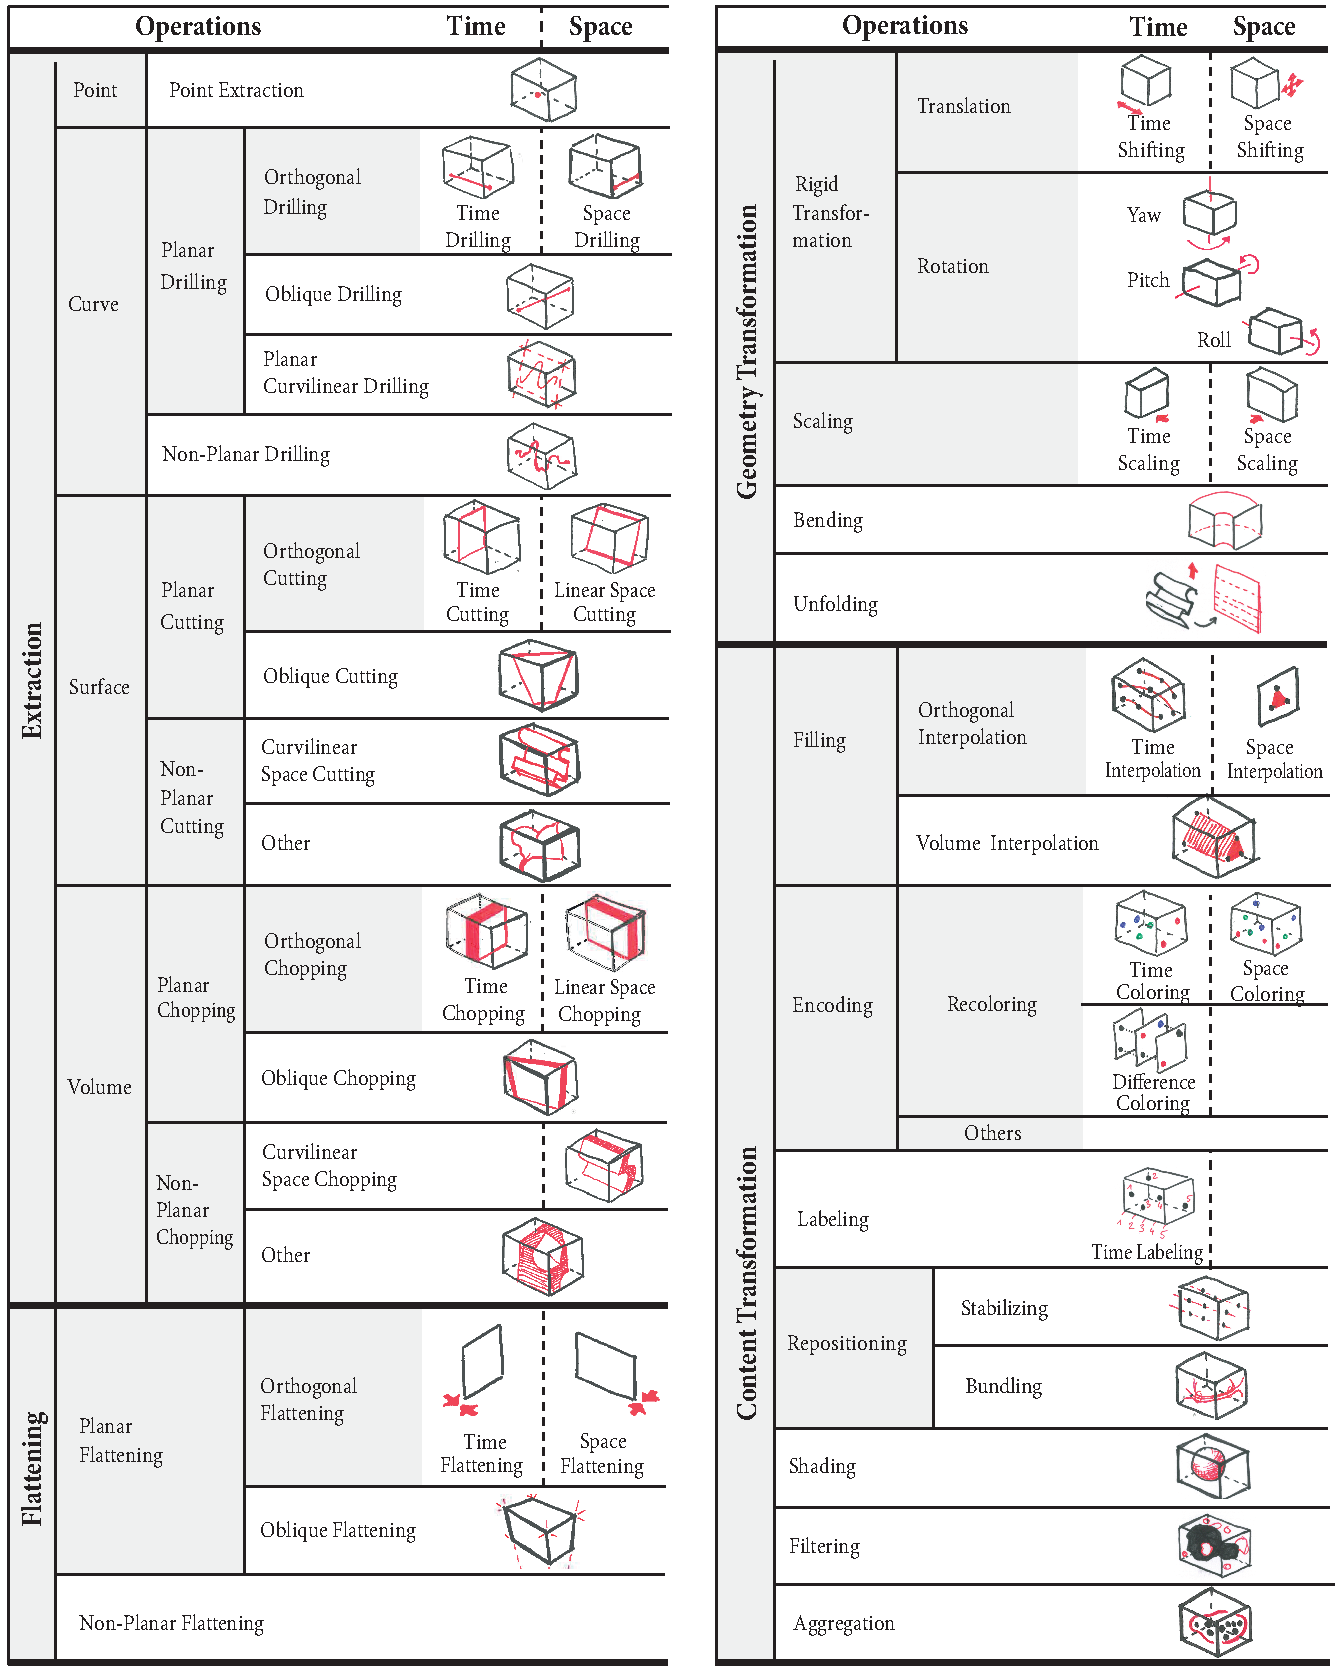
\includegraphics[width=1\textwidth]{images/bach2014reviewFull}
\caption{Taxonomy of Space-Time cube operations created by Bach et al.\ \cite{bach2014review} Each operation gives a representation of how the operation may work. Bold font indicates complete operations. Gray shading indicates non-leaf nodes. Image courtesy of Bach et al.\ \cite{bach2014review}} \label{fig: bach2014review}
\end{center}
\end{figure}

%%\item \textit{Classification Dimensions:}
%\begin{itemize}
%\item[X:] Operations, Time, Space
%\item[Y:] Extraction: [Point Extraction, Planar Drilling, Planar Cutting, Non-Planar Cutting, Planar Chopping, Non-Planar Chopping],\\
%Geometry Transformation: [Rigid Transformation, Scaling, Bending, Unfolding],\\
%Content Transformation: [Recoloring, Labeling, Repositioning, Shading, Filtering, Aggregation],\\
%Flattening, Filling.
%\item \textbf{Site:} \url{http://spacetimecubevis.com/}
%\item \textbf{Papers:} 91 Papers cited in Survey \{1970-2013\}\\
%\end{itemize}

%\item \textit{Unsolved Problems/Future Research:}
There are many open research areas that are discussed within the paper. Some of these include interaction techniques such as focus+context to use with different operations, research into operations for extended data dimensions, and understanding which operation is most appropriate for a given task.

%\end{enumerate}

\subsubsection{Geospatial Focused Surveys}
This section focuses on surveys that examine geo-spatial visualization. The section provides an understanding, and classification, of tasks for cartograms, a view of geospatial traffic data, and another review of the use of cartographic visualization in information visualization.

%Title: \textit{A Survey of Traffic Data Visualization} by Chen et al. \cite{chen2015survey}
%\begin{enumerate}
%\item \textit{The Concept:}
Chen et al.\ analyze various ways traffic data can be recorded as well as some different approaches that are brought forward to depict a combination of spatial, temporal, dimensional, and categorical visualization \cite{chen2015survey}.
They systematically review how traffic data is captured. This is divided into three unique categories: Location-Based, which records data as it appears at a fixed point, or sensor range; Activity-Based, which may record data when a specific event is started or finished; Device-Based, recording from a device which records information periodically such as a GPS. Each of these has their own unique benefits and uses. Each data type can be broken down into the four types mentioned previously: spatial; temporal; dimensional; and categorical.
%\item \textit{The Scope:}
Chen et al.\ begin by looking at how the traffic data can be captured and discuss the different ways this data can be processed. The main focus of the survey is how the data is visualized. The paper provides examples of usual design for time, spatial properties, spatio-temporal data, and multi-property data.

%\item \textit{Classification:}
To further improve the taxonomy of traffic data, Chen et al.\ structure the visual design types into the three main goals: Situation-Aware Exploration and Prediction; Pattern Discovery and Clustering; and Visual Monitoring of Traffic Situations. These goals are clearly explained and then presented with relevant examples \cite{chen2015survey}. 

\begin{figure}[t]
\begin{center}
\includegraphics[width=1\textwidth]{images/chen2015survey.png}
\caption{The taxonomy displays different data types with their potential properties. These are then categorized into three data types: Numerical; Categorical; or Textual. Examples of related literature are also given. Courtesy of Chen et al.\ \cite{chen2015survey}}
\end{center}
\end{figure}

%\item \textit{Classification Dimensions: }
%\begin{itemize}
%\item[X:]Tools, Characteristics, Datasets, Platform.
%\item[Y:]Tasks: [Situation-aware exploration and prediction; Pattern discovery and clustering; traffic situations monitoring.]
%\item \textbf{Papers:} 96 Papers cited in Survey \{1991-2014\}\\
%\end{itemize}

%\item \textit{Unsolved Problems}
Chen et al.\ present analysis of situation-aware and immersive environments, as well as the design of huge spatio-temporal analysis of online or streamed data, as open challenges in the field. Visual Analysis of heterogeneous data, social transportation as an example, is another area that requires more focused research.
%\end{enumerate}

%Title: \textit{Task Taxonomy for Cartograms} by Nusrat and Kobourov \cite{nusrat2015task}.
%\begin{enumerate}
%\item \textit{The Concept:}
A cartogram is a type of visualization that aims to combine statistical and geographical information where areas are scaled dependent on statistical proportions. Nusrat and Kobourov study the effectiveness of cartograms as a visualization tool, as well as compare the effectiveness of different cartogram methods. The paper presents a set of cartographic visualization tasks and their application to information visualization \cite{nusrat2015task}.
%\item \textit{The Scope:}
Nusrat and Kobourov begin by providing an overview of cartograms, with related literature for those who want to expand their knowledge of the subject. They then present their design space for cartographic tasks and visual goals for cartogram usage. Both of these are coupled with clear examples of when they could be selected. 

%\item \textit{Classification:}
Nusrat and Kobourov classify tasks by reviewing two hierarchical dimensions, analytic tasks such as identification, location, sorts and clustering (see Figure \ref{fig: nusrat2015task}). The second axis maps visualization goals which includes the goal of the visualization, how a task is carried out, features of the task, and the cardinality. 

\begin{figure}[t]
\begin{center}
\includegraphics[width=1\textwidth]{images/nusrat2015taskFullp}
\caption{Task taxonomy for cartogram visualization courtesy of Nusrat and Kobourov \cite{nusrat2015task}.} \label{fig: nusrat2015task}
\end{center}
\end{figure}

%\item \textit{Classification Dimensions:}
%\begin{itemize}
%\item[~]\begin{center} Classification Structure: 2D Hierarchical \end{center}
%%\item[List:]
%\item[Y:] Analytic Tasks: [Recognize, Detect Change, Compare, Find top-k, Filter, Cluster, Locate, Find-Adjacency, Summarise, Identify]
%\item[X$^1$:] Goals: [Query, Search, Extract]
%\item[X$^2$:] Means: [Map Relation, Data Relation, Navigation, Derive]
%\item[X$^3$:] Characteristics: [Low-Level, High-Level]
%\item[X$^4$:] Cardinality: [Single, Multiple, All]
%
%
%\item \textbf{Site:} n/a \url{}
%\item \textbf{Papers:} 40 Papers cited in Survey \{1934-2015\}\\
%
%\end{itemize}

%\item \textit{Unsolved Problems/Future Research:}
%n/a
%\end{enumerate}


%Title: \textit{The State of the Art in Cartograms} by Nusrat and Kobourov. \cite{nusrat2016state}
%\begin{enumerate}
%\item \textit{The Concept:}
Nusrat et al.\ follow-up their previous survey with an extended version \cite{nusrat2016state}.
%\item \textit{The Scope:}
They start by presenting a history of cartographic visualization, beginning with their origins in 1870. The paper examines the literature surveys related to cartograms, discussing what is presented in each, before discussing the different design-types of cartographic layouts as well as a task taxonomy extension of `\textit{Task Taxonomy for Cartograms}' by Nusrat and Kobourov \cite{nusrat2015task}, their applications, and their effectiveness.

%\item \textit{Classification:}
They introduce the three major design dimensions of cartographic visualization:
Statistical accuracy, geographical accuracy, and topological accuracy. In addition, cartograms are sub-divided into four different types which include contiguous, non-contiguous, Dorling, and rectangular cartograms.

\begin{figure}[p]
\begin{center}
\includegraphics[width=1\textwidth]{images/nusrat2016state.png}
\caption{A 2D systematic overview of different types of cartograms, displayed with their categorizations. Courtesy of Nusrat and Kobourov \cite{nusrat2016state}} \label{fig: nusrat2016state}
\end{center}
\end{figure}

%\item \textit{Classification Dimensions:}
%\begin{itemize}
%\item[X:] Focus: Statistics, Continguity, Geography, Topology, Example
%\item[Y:] Cartogram Type
%\item \textbf{Site:} \url{http://cartogram.cs.arizona.edu/survis-cartogram/}
%\item \textbf{Papers:} 163 Papers cited in Survey \{1932-2016\}\\
%\end{itemize}

%\item \textit{Unsolved Problems/Future Research:}
Nusrat and Kobourov pose a multitude of areas for future cartogram research. Firstly, some of the design dimensions are under-utilized, which could facilitate a paper comparing usage with less used cartographic layouts. Cartograms normally only excel in one of the three design dimension, and a study to mitigate errors in the other two dimensions may allow for a better understanding of cartogram usage. Some other areas of interest are the mapping of multivariate data, memorability and recall within cartograms, uncertainty within cartograms, and 3D cartographic visualization.

%\end{enumerate}

\subsection{Coordinated Multiple View (CMV) Surveys }
Coordinated Multiple Views (CMVs) surveys focus on literature that examines the coordination or linkage between multiple views. This section summarizes two papers related to the subject. The first reviews the use of composite visualization and the second provides an understanding of multi-faceted graph visualization.

%Title: \textit{Exploring the Design Space of Composite Visualization} by Javed and Elmqvist. \cite{javed2012exploring}.
%\begin{enumerate}
%\item \textit{The Concept:}
Javed and Elmqvist examine different Composite Visualization Views (CVVs), which are defined as \textit{"a visual composition of two or more visual structures in the same view,"} and present their CVV design patterns created via a literature survey \cite{javed2012exploring}.
%\item \textit{The Scope:}
They start by discussing different CVVs, including their design patterns  and existing formalisms. This is followed with an in-depth look at the different types of views (juxtaposed, integrated, superimposed, etc), with examples of each. They then present their design space and guidelines, as well as their 1-N classification table.

%\item \textit{Classification:}
The authors look at different techniques and how the visualization's relations are classified. The grouping looks at the result of merging two visual designs, the composite relation (juxtaposed, integrated, superimposed, overloaded, nested), as well as what data-relation is created (item-item, item-group, etc).

\begin{figure}[t]
\begin{center}
\includegraphics[width=1\textwidth]{images/javed2012exploring}
\caption{ Classification of common composite visualization techniques \cite{javed2012exploring} .} \label{fig: javed2012exploring}
\end{center}
\end{figure}

%\item \textit{Classification Dimensions:}
%\begin{itemize}
%\item[~]\begin{center} Classification Structure: 2D \end{center}
%
%\item[X$^1$:] Visualization A
%\item[X$^2$:] Visualization B
%\item[X$^3$:] Spatial Relation
%\item[X$^4$:] Data Relation
%\item[Y:] Technique
%
%\item \textbf{Site:} n/a \url{}
%\item \textbf{Papers:} 45 Papers cited in Survey \{1885-2013\}\\
%
%\end{itemize}

%\item \textit{Unsolved Problems/Future Research:}
Javed and Elmqvist suggest their design patterns are limited to literature reviewed and therefore work can be invested into extending their framework. The design pattern is also limited to only spatial relation and does not look at other composite visualization views, such as interaction or animation.
%\end{enumerate}

%Title: \textit{A Survey of Multi-faceted Graph Visualization} by Hadlak et al. \cite{hadlak2015survey}
%\begin{enumerate}
%\item \textit{The Concept:}
Many surveys focus on only a single additional facet in order to classify graphing techniques. Hadlek et al.\ aim to build on existing surveys in order to create a more in-depth observation of four common facets: partitions, attributes, time, and space. Each of these characteristics are discussed based on their relationship as well as examples of how these graphs can be represented depending on the hierarchy.
%\item \textit{The Scope:}
Hadlek et al.\ focus on an output oriented perspective, and optimize facet selection by focusing on their composition. These compositions are given a representative visualization (seen in Figure \ref{fig: hadlak2015survey}) to discuss in detail in the content of the survey. Hadlek et al.\ analyse visual design of the graph structure with a single additional facet and graph structure with multiple additional facets. These are sub-divided for each common facet. This is followed by analyzing multiple instances of graph facets.

%\item \textit{Classification:}
Each graph structure is split into five combinations. Whilst looking at the spatial composition, an example is given for structure as the base representation, partitions as the base representation, or a balanced representation. A temporal composition has an example for either structure as the base representation or partitions as the base representation.

\begin{figure}[t]
\begin{center}
\includegraphics[width=0.8\textwidth]{images/hadlak2015survey.png}
\caption{Examples of multiple facet representations within visualization. Courtesy of Hadlak et al.\ \cite{hadlak2015survey}} \label{fig: hadlak2015survey}
\end{center}\vspace{-0.5cm}
\end{figure}

%\item \textit{Classification Dimensions:}
%\begin{itemize}
%\item[X:] Representation: [Structure as base, Balanced, Time as Base]
%\item[Y:] Compisition: [Spatial, Temporal]
%\item \textbf{Papers:} 133 Papers cited in Survey \{1990-2015\}\\
%
%\end{itemize}

%\item \textit{Unsolved Problems/Future Research:}
The paper notes the exploration of geo-spatial graph visualization, by reviewing output or task taxonomy, has yet to be published. Hadlek et al.\ also point out that some of the facets discussed had very sparse usage such as temporal compositions. Finally, only four facets were examined but there are many other extensions such as provenance, uncertainty, heterogeneity, or text/annotations that have little-or-no exposure which could be a new thread of research to investigate.
%\end{enumerate}

\subsection{Real-World and Applications}
Many literature surveys focus on real-world scenarios and applications. This area covers a wide range of surveys including finance, health-care, security, systems, software visualization, and visualization frameworks.
\subsubsection{Finance Focused Surveys}
This section has a focus on survey papers related to finance visualization. The survey summarizes one paper focused on different sources of financial data and how they are visualized.

%Title: \textit{A Survey on Visual Analysis Approaches for Financial Data} by Ko et al.\ \cite{ko2016survey}
%\begin{enumerate}
%\item \textit{The Concept:}
Ko et al.\ perform and present a study of visualization and visual analytics of financial data. Economy is an important field for any business which has led to financial data being a popular topic for visualization in industries. They aim to utilize existing papers in order to help researchers design better systems and understand new research fields within the area \cite{ko2016survey}.
%\item \textit{The Scope:}
After discussing the survey scope, Ko et al.\ explore the types of data analyzed and some data sources for each. Some examples of this include stock data, transaction data, and fund data. The paper derives a classification of techniques and provides examples of these uses before examining the interaction methods and evaluation methods. This is followed by an evaluation of the papers.

%\item \textit{Classification:}
Ko et al.\ examine multiple ways to classify the gathered information. The first classification tests the type of data used by each paper, which indicates a heavy focus on stock data. The second classification discusses papers based on automated techniques, such as K-means. The third looks at visualization techniques, based on Keim's technique taxonomy \cite{keim2002information} (see Figure \ref{fig: ko2016survey}). The fourth categorization considers interaction methods and the final organization examines evaluation methods.

\begin{figure*}[t]
\begin{center}
\includegraphics[width=1\textwidth]{images/ko2016surveyFull}
\caption{Ko et al.'s Categorization of surveyed papers via Keim's visualization techniques taxonomy \cite{ko2016survey,keim2002information} .} \label{fig: ko2016survey}
\end{center}
\end{figure*}

%\item \textit{Classification Dimensions:}
%\begin{itemize}
%\item[~]\begin{center} Classification Structure: 2D (x5) \end{center}
%%\item[List:]
%\item[X:] Paper
%\item[Y$^1$:] Data Sources: [Stock, Fund, Econ. Indi., Trans, Risk, Company Info]
%\item[Y$^2$:] Automated Techniques: [K-means, SOM, MDS, PCA, Sampling, Moving Avg., Regression, Decision Tree, Specific Models]
%\item[Y$^3$:] Visualization Techniques: [Std (2D), Std (3D), GT, Iconic, Dense Pixel, Stacked]
%\item[Y$^4$:] Interaction Methods: [Select, Explore, Reconfigure, Encode, Abstract, Filter, Connect]
%\item[Y$^5$:] Evaluation Methods: [Use Case, Case Study, User Feedback, User Study, Performance]
%
%\item \textbf{Site:} n/a \url{}
%\item \textbf{Papers:} 50 Papers cited in Survey \{1992-2014\}\\
%\footnotesize * literal count of cited papers and not papers surveyed.\\
%\end{itemize}

%\item \textit{Unsolved Problems/Future Research:}
They propose that there are nine more business domains which could have their visual analytics reviewed such as economic analysis, financial risk management, and portfolio management. They also discuss the lack of research into company performance with financial data and suggest this as an open field. An important area for research is with automated visualization techniques, which industry experts believe are important to facilitate a richer depth of information. The final point they discuss is the use of heterogeneous data to enable improved prediction models.

%\end{enumerate}
\subsubsection{Security-based Literature Surveys}
This section includes survey papers that present security systems. One features a focus on visualization systems for network security and  another on malware analysis.

%Title: \textit{A Survey of Visualization Systems For Network Security} by Shiravi et al.\ \cite{shiravi2012survey}.
%\begin{enumerate}
%\item \textit{The Concept:}
Shiravi et al.\  provide a comprehensive overview of network security visualization and present data sources for each. The paper also provides a taxonomy that includes literature across five use-cases \cite{shiravi2012survey}.
%\item \textit{The Scope:}
They present a table that provides potential data sources for security visualization before giving an in-depth view of five use-cases for reviewing network security and their related papers. The use-cases are host/server monitoring, internal/external monitoring, port activity, attack patterns, and routing behavior.

%\item \textit{Classification:}
The taxonomy takes the form of a 2D table, sub-divided into five sections representing the five use-cases. The taxonomy reviews the type of visualization techniques and data source of each research paper. It also includes the number of citations a paper has to emphasize systems that have more references, as well as signifying whether the system is available online.

\begin{figure}[p]
\begin{center}
\includegraphics[width=0.8\textwidth]{images/shiravi2012survey}
\caption{Taxonomy of Security Visualization Systems, divided into different use-cases. Created by Shiravi et al.\ \cite{shiravi2012survey} .} \label{fig: shiravi2012survey}
\end{center}
\end{figure}

%\item \textit{Classification Dimensions:}
%\begin{itemize}
%\item[~]\begin{center} Classification Structure: 3D Hierarchical \end{center}
%%\item[List:]
%\item[X$^1$:] Visualization Technique
%\item[X$^2$:] Data Source
%\item[X$^3$:] Number of Citations
%\item[Y:] Visualization System
%\item[Z:] Online Availability
%
%\item \textbf{Site:} n/a \url{}
%\item \textbf{Papers:} 90 Papers cited in Survey \{1995-2011\}\\
%
%\end{itemize}

%\item \textit{Unsolved Problems/Future Research:}
Shiravi et al.\ present future research topics including situation awareness in presenting information, user experience evaluation, scalablity, occlusion in network security, privacy preservation and   novel ways to provide 3D imagery of the data.

%\end{enumerate}

%Title: \textit{A Survey of Visualization Systems for Malware Analysis} by Wagner et al. \cite{wagner2015survey}
%\begin{enumerate}
%\item \textit{The Concept:}
Wagner et al.\ present a systematic overview and classification of malware visualization systems used for visual analysis. The field is gaining more and more interest due to the increasing threat of malware attacks on user systems. Malware is defined as \textit{"any software that does something that causes harm to a user, computer or network"} \cite{wagner2015survey}.
%\item \textit{The Scope:}
They focus on malware systems for visual analysis. They first provide tools, discussed as \textit{data providers}, and provide a comparison of their usage. They present their malware visualization taxonomy and categorize each data provider in a number of different classification groups.

%\item \textit{Classification:}
Wagner et al.\  create three categories for malware visualization systems: (1) Individual malware analysis which enables the system to look at a single malware sample and learn about its individual behavior. (2) Malware comparison which facilitates comparison of a range of malware for viewing. (3) Malware summarisation that outlines the behavior of different malware samples (see Figure \ref{fig: wagner}).

\begin{figure*}[t]
\begin{center}
\includegraphics[width=1\textwidth]{images/wagner2015survey.png}
\caption{The 1D malware visualization taxonomy courtesy of Wagner et al.\ \cite{wagner2015survey}} \label{fig: wagner}
\end{center}
\end{figure*}

%\item \textit{Classification Dimensions:}
%\begin{itemize}
%\item[X:] Malware Analysis Tool
%\item[Y:] Base Data, Data Format, Visualization Techniques, Mapping and Representation Space, Temporal Aspects, Interactivity, Tasks.
%\item \textbf{Papers:} 91 Papers cited in Survey \{1974-2015\}\\
%\end{itemize}

%\item \textit{Unsolved Problems/Future Research:}
They find that malware visualization is cleanly partitioned between each classification category and believe more work needs to be done in creating a connection between  categories. Using different systems could cause unnecessary overlap for users which could be minimized with a system that could move through this categorization. Some other challenges in the field include the integration of more data sources, a stronger understanding of the requirements for malware visualization, enabling expert analysis and externalization, and an increased focus on the relation between analysis and visualization for malware.

%\end{enumerate}
\subsubsection{Systems-based Surveys}
This section focuses on Surveys that have an emphasis on classifying systems. We summarize one survey paper in this section which looks at performance visualization of large-scale systems.


%Title: \textit{Performance Visualization for Large-scale Computing Systems} by Gao et al.\ \cite{gao2011performance}
%\begin{enumerate}
%\item \textit{The Concept:}
Gao et al.\ present a review on papers designated for researching performance visualization on large-scale systems. Gao et al.\ define performance visualization as \textit{`the use of graphical display techniques for the visual analysis of performance data'}\cite{gao2011performance}. The paper aims to shed light on open research areas, and increased discussion on the design of visual tools for these systems. 
%\item \textit{The Scope:}
The paper provides a brief background of performance visualization and how it functions.

%\item \textit{Classification:}
Gao et al.\ classify performance visualization techniques using four main categories. Simple visual structures which include statistical charts with one or two variables, composed visual structures that include a combination of simple chart views, interactive visual structures featuring structures that provide a variety of user interactions, and focus+context which refers to visualizations with mapping that is automatically modified without the need of user interaction.


\begin{figure}[t]
\begin{center}
\includegraphics[width=1\textwidth]{images/gao2011performance}
\caption{A classification of performance visualization techniques courtesy of Gao et al.\ \cite{gao2011performance}.} \label{fig: gao2011performance}
\end{center}
\end{figure}

%\item \textit{Classification Dimensions:}
%\begin{itemize}
%\item[~]\begin{center} Classifcation Structure: Hierarchical \end{center}
%\item[L:]Simple Visual Structures: ["Pie Charts, Distribution, Box Plots, Kiviat Diagrams", "Timeline Views", "Information Typologies", "Information Landscape Trees \& Networks"],\\
%Composed Visual Structures: ["Single-Axis Composition", "Double-Axis Composition", "Case Composition"],\\
%Interactive Visual Structure: ["Interaction through controls", "Interaction through image"]\\
%Focus+Context Visual Structures: ["Macro-micro composite view"].
%
%
%\item \textbf{Site:}  n/a \url{}
%\item \textbf{Papers:} 21 Papers cited in Survey \{1923-1998\}\\
%\end{itemize}

%\item \textit{Unsolved Problems/Future Research:}
Some future work areas presented by Gao et al.\ include scalability, user studies, and the synthesis of high-level context with low-level detail.

%\end{enumerate}
\subsubsection{Software Visualization Surveys}
Software Visualization papers focus on visualizing aspects of software creation. Diehl defines the topic as follows:\textit{`Software visualization encompasses the development and evaluation of methods for graphically representing different aspects of software, including its structure, its execution, and its evolution'} \cite{diehl2007software}. The SoS summarizes one recent survey paper in this section that focuses on the static aspects of software visualization.

%Title: \textit{Visualization of the Static Aspects of Software: A Survey} by Caserta and Zendra \cite{caserta2011visualization}.
%\begin{enumerate}
%\item \textit{The Concept:}
Caserta and Zendra categorize visualization techniques that represent the static aspects of software and it's evolution. The paper defines visualization of the static aspects of software as `\textit{visualizing software as it is coded, and dealing with information that is valid for all possible executions of the software}' \cite{caserta2011visualization}. Evolution of software adds a temporal dimension to the visualization of the static aspects of software.
%\item \textit{The Scope:}
The paper provides a guide to papers that feature code-line-centered visualization, class-centered visualization, architecture visualization, and the visualization of software evolution. They provide examples of different types of visual design for each and how they may be applied.

%\item \textit{Classification:}
The hierarchical, 1-N, classification presents the representation and visualization techniques used for each paper, and shows how they fit into their taxonomy (see Figure \ref{fig: caserta2011visualization}).

\begin{figure}[t]
\begin{center}
\includegraphics[width=1\textwidth]{images/caserta2011visualization}
\caption{Caserta and Zendra present a table that classifies methods that visualise the static aspects of software and the associated literature \cite{caserta2011visualization} .} \label{fig: caserta2011visualization}
\end{center}
\end{figure}

%\item \textit{Classification Dimensions:}
%\begin{itemize}
%\item[~]\begin{center} Classification Structure: 2D Hierarchical \end{center}
%%\item[List:]
%\item[Z$^1$:] Aspects of Software Visualization: [Static Aspects, Static Aspects + Time]
%\item[X$^2$:] Level: [Code-line-centered, Class-Centered, Architecture]
%\item[X$^3$:] Focus: [Line Properties, Functioning/Metrics, Organisation, Relationships, Metrics, Changes, Orginizational Changes, Metrics Evolution]
%\item[X$^4$:] Visualization Technique
%\item[X$^5$:] Representation
%
%
%\item \textbf{Site:} n/a \url{}
%\item \textbf{Papers:} 192 Papers cited in Survey \{1979-2011\}\\
%
%\end{itemize}

%\item \textit{Unsolved Problems/Future Research:}
Caserta and Zendra propose that it would be beneficial to invest research into usability evaluation to find the most effective ways to visualize the static aspects of software. There is also limited research in navigation and interaction for 3D visualization within the field.

%\end{enumerate}

\subsubsection{Surveys of Frameworks}
This section examines the review of frameworks, which is defined as \textit{`a basic structure underlying a concept'} \cite{frameworkdictionary}. The section covers two surveys: the first presents a design framework survey for bi-cluster visualizations and the second presents a framework for emphasis in visualizations.

%Title: \textit{A Five-Level Design Framework for Bicluster Visualizations} by Sun et al. \cite{sun2014five}
%\begin{enumerate}
%\item \textit{The Concept:}
Sun et al.\ provide a survey focused on bi-cluster visualization, design considerations, and applications. Bi-clusters \textit{"provide a rich high-level abstraction that represents coordinated relationships between groups of entities of different types"} \cite{sun2014five}. The advantages and disadvantages are compared, and a five-level relationship is presented to assist in design options that support user-tasks.
%\item \textit{The Scope:}
The paper describes the concept of bi-clustering and the five relationship levels of the bi-cluster visualization design framework. These include: entity level (single entity relationships), group level (entity group relationships), bi-cluster level (coordinated relationships), chain level (chained coordinated relationships), and the schema level (schema level relationships). The paper also examines four levels of interaction design: readability, navigation, parameter, and object level.

%\item \textit{Classification:}
Sun et al.\ provide a summary of the five-level design framework for bi-cluster visualization. This incorporates the interaction design level, major tasks, design choice, and trade-offs.

\begin{figure}[t]
\begin{center}
\includegraphics[width=1\textwidth]{images/sun2014five.png}
\caption{Design framework associated with bicluster visualization. Courtesy of Sun et al.\ \cite{sun2014five}.} \label{fig: sun2014five}
\end{center}
\end{figure}

%\item \textit{Classification Dimensions:}
%\begin{itemize}
%\item[~]\begin{center} Classifcation Structure: 2D Hierarchical \end{center}
%\item[X:] Major Tasks, Design Choices, Pros, Cons.
%\item[Y:] Relations: [Entity Level, Group Level, BiCluster Level, Chain Level, Schema Level]
%\item \textbf{Site:} n/a \url{}
%\item \textbf{Papers:} 93 Papers cited in Survey \{1972-2014\}\\
%\end{itemize}


%\item \textit{Unsolved Problems/Future Research:}
They identify three challenges in the field. The first challenge is the creation of an example  that implements design options across all five levels of the framework. The second challenge discusses traversal between the different levels. The final challenge suggests optimal layout of bi-cluster chains in visualization.

%\end{enumerate}

%Title: \textit{Formalizing Emphasis in Information Visualization} by Hall et al.\ \cite{hall2016formalizing}
%\begin{enumerate}
%\item \textit{The Concept:}
Hall et al.\ present a mathematical Framework for Information Visualization Emphasis (FIVE) by reviewing existing emphasis literature and frameworks \cite{hall2016formalizing}. Some examples of emphasis provided include highlighting regions of interest, animating data points, and altering the size of data points.
%\item \textit{The Scope:}
They first present a language for emphasizing sub-sets of data, and present a table displaying how their framework compares to previous solutions (see Figure \ref{fig: hall2016formalizing}). The paper then discusses different types of emphasis effects and how they can be used such as position, color, motion and transparency. Finally, the paper discusses the opportunities to use FIVE and some future directions for research.

%\item \textit{Classification:}
The frameworks are split into three categories. (1) \textit{Magnification} - papers that describe magnification emphasis effects. (2) \textit{Beyond magnification} - papers describing non-magnification emphasis effects. (3) \textit{Data suppression} - papers that focus on the creation of emphasis effects through data suppression. 

\begin{figure}[p]
\begin{center}
\includegraphics[width=0.8\textwidth]{images/hall2016formalizingFull}
\caption{Hall et al.\ present a table used to classify previous emphasis frameworks to diagnose what types of emphasis are discussed, and compare them to FIVE \cite{hall2016formalizing}  .} \label{fig: hall2016formalizing}
\end{center}
\end{figure}

%\item \textit{Classification Dimensions:}
%\begin{itemize}
%\item[~]\begin{center} Classification Structure: 4D \end{center}
%%\item[List:]
%\item[X:] Frameworks
%\item[Y:] Year, Size, Position, Depth, Illumination, Transparency, Blur/Clearness, Color Hue, Color Saturation, Color Value, Motion, Texture, Orientation, Flicker, Shape, Data Points, Data Dimensions.
%\item[Z$^1$:] Texture: [Variable discussed, Variable alluded, Variable not discussed]
%\item[Z$^2$:] $*$ - early visual variables,\\ $**$ - recent visual variables
%
%\item \textbf{Site:} n/a \url{}
%\item \textbf{Papers:} 81 Papers cited in Survey \{1982-2016\}\\
%\end{itemize}

%\item \textit{Unsolved Problems/Future Research:}
They provide four areas for future work: creating emphasis effects using under-explored visual variables and time variation, exploring alternative ways to vary data point prominence to create emphasis effects, providing a richer space of how to define and implement emphasis effects, and conducting empirical studies of emphasis effects.

%\end{enumerate}

\subsection{Overview Surveys}
Surveys that attempt to cover information visualization as a whole are presented here. This section summarizes two papers that review recent advancements in information visualization.

We summarize one survey that reviews the use of interactive lenses in visualization.
%Title: \textit{A Survey on Interactive Lenses in Visualization} by Tominski et al. \cite{tominski2014survey}
%\begin{enumerate}
%\item \textit{The Concept:}
Tominski et al.\ aim to analyze the use of interactive lenses in the context of visualization by reviewing the different techniques used to create lenses, whilst also helping researchers identify when to use interactive lenses. They discuss applicable data types such as geo-spatial data, why incorporating lenses is beneficial to the user experience, and some important techniques to be aware of if you are interested in this type of visualization. An interactive lens is defined as \textit{`to provide an on
demand alternative visual representation of the data underlying a local area of the screen'} \cite{tominski2014survey}.
%\item \textit{The Scope:}
After introducing the model of the interactive lens as well as the discussion of lens usage, they segment the research into interaction types. This includes examination of mouse and keyboard interaction, touch and multi-touch interaction, tangible interaction, tangible views and spatial interaction, gaze-based interaction and head tracking. \cite{tominski2014survey}

%\item \textit{Classification: }
The taxonomy of Tominski et al's survey examines both the data types that each visualization technique demonstrates (temporal, geospatial, flow, etc.), as well as the task that is achieved using it (across a total of 43 papers). This taxonomy enables discussion of possible future work such as the use of lenses for multi-user work (see Figure \ref{fig: tominski2014survey}).

\begin{figure}[p]
\begin{center}
\includegraphics[width=0.85\textwidth]{images/tominski2014surveyFull}
\caption{Lens Techniques categorised according to data types and task. Courtesy of Tominski et al.\ \cite{tominski2016interactive}}\label{fig: tominski2014survey}
\end{center}
\end{figure}\vspace{-0.2cm}

%\item \textit{Classification Dimensions: }
%\begin{itemize}
%\item[X:]Data Type: [ Temporal, Geo-Spatial, Flow, Volume, Graph, Document],\\ Tasks: [Select, Explore, Reconfigure, Encode, Abstract \& Elaborate, Filter, Connect].
%\item[Y:] Magic Lens Techniques
%\item \textbf{Papers:} 43 Papers cited in Survey \{1983-2014\}
%\end{itemize}

%\item \textit{Unsolved Problems}
After reviewing some survey notes, they suggest that the need for more dynamic lenses with flexibility is an important design note as well as useful for a more varied use of functionality. Although mentioned in the survey, Tominski et al.\ would like to further investigate the development of multi-user or shared lenses, due to the growth in high-resolution and interactive displays. Finally, the idea of lens tool kits is an important focus area. Lenses are globally recognized visualization types but are in low use due to how interwoven they are with visualizations. With big data becoming a strong focus, this is something that needs further development. Tominski et al.\ also provide an extended version of the classification (see Figure \ref{fig: tominski2014survey}) \cite{tominski2016interactive}.

%\end{enumerate}
%Title: \textit{A Survey on Information Visualization - Recent Advances and Challenges} by Liu et al. \cite{liu2014survey}
%\begin{enumerate}
%\item \textit{The Concept:}
Liu et al.\ create a comprehensive study on the domain of information visualization. The aim of the paper is to derive an organization of the field, describing features, goals and state-of-the-art approaches for each category \cite{liu2014survey}.
%\item \textit{The Scope:}
The paper opens by examining the visualization pipeline and classification schemes. They proceed to present their 1-N taxonomy of the literature landscape within recent years, and present each topic whilst giving examples of papers in the related area. This continues on to communicating some technical challenges.

%\item \textit{Classification:}
Liu et al.\ break their taxonomy down into four main categories: empirical methodologies, interactions, frameworks, and applications. These categories are sub-divided into sub-categories. The classification has a lot of overlap with our organization. 


%\begin{figure}[ht]
%\begin{center}
%\includegraphics[width=0.5\textwidth]{images/liu2014survey.png}
%\caption{A taxonomy of InfoVis techniques created by Liu et al.\ \cite{liu2014survey}.} \label{fig: liu2014survey}
%\end{center}
%\end{figure}

%\item \textit{Classification Dimensions:}
%\begin{itemize}
%\item[~]\begin{center} Classifcation Structure: Hierarchical \end{center}
%\item[L:] Emperical Methods: [Model, Evaluation],\\
%Interactions: [WIMP interactions, Post-WIMP interactions],\\
%Frameworks: [Systems and Frameworks],\\
%Applications: [Graph Visualization, Map Visualization, Multivariate Data Visualization].
%\item \textbf{Site:} n/a \url{}
%\item \textbf{Papers:} 170 Papers cited in Survey \{1981-2012\}\\
%\end{itemize}

%\item \textit{Unsolved Problems/Future Research:}
Liu et al.\ describe an abundance of open research areas including usability, scalability, heterogeneous data, real-time visualization, and uncertainty.

%\end{enumerate}


%%%%%%%%%%%%%%%%%%%%%%%%%%%%%%%%
%%%CURRENT SURVEY SUMMARIES %%%%
%%%%%%%%%%%%%%%%%%%%%%%%%%%%%%%%






%%%%%%%%%%%%%%%%%%%%%%%%%%%%%%%%
%%%CURRENT SURVEY SUMMARIES %%%%
%%%%%%%%%%%%%%%%%%%%%%%%%%%%%%%%

\section{Analysis of Future Work}
At the end of most survey papers, it is common for the authors to discuss future areas of work that are discovered over the course of the survey. These challenges and research directions have been compiled using SurVis, an online literature browser \cite{beck2016visual,surVis}. This enables us to find a number of future research areas within Information Visualization.

\begin{table}[p]
\scriptsize
\ra{1.15}
\centering


\begin{tabular}{|r|c|c|c|c|c|c|c|c|c|c|c|c|}

\rot{ \textbf{\textsc{Literature:}}}&\rot{\textsc{Evaluation}}&\rot{ \textsc{Missing Scenarios}}&\rot{ \textsc{Scalability}}&\rot{ \textsc{Interaction Techniques}}&\rot{ \textsc{Extended Data Dimensions}}&\rot{ \textsc{Tasks}~~~}&\rot{ \textsc{Tools}}&\rot{ \textsc{Fuzzyness \& Uncertainty}}&\rot{ \textsc{Time-Varying Data}}&\rot{ \textsc{Design Guidelines}}&\rot{ \textsc{heterogeneity}}\\ \hline
\fillCellSubHeader \cite{ahn2014task}					&&\fillItem &\fillItem &&&&&&\fillItem &&\\ \hline
\fillCellSubHeader \cite{alsallakh2014visualising}		&\fillItem &\fillItem &\fillItem &\fillItem &&&\fillItem &\fillItem &\fillItem &&\\ \hline
\fillCellSubHeader \cite{bach2014review}				&\fillItem &&&\fillItem &\fillItem &\fillItem &&&&&\\ \hline
\fillCellSubHeader \cite{beck2014state}				&\fillItem &\fillItem &\fillItem &\fillItem &\fillItem &&&&&&\\ \hline
\fillCellSubHeader \cite{behrisch2016matrix}			&\fillItem &&&&&&\fillItem &&&&\\ \hline
\fillCellSubHeader \cite{bertini2011quality}			&\fillItem &&\fillItem &&&&&&&&\\ \hline
\fillCellSubHeader \cite{borgo2013glyph}				&&&&&&&\fillItem &&&&\\ \hline
\fillCellSubHeader \cite{caserta2011visualization} 	&\fillItem &&&\fillItem &&&&&&&\\ \hline
\fillCellSubHeader \cite{chen2015survey}				&&&&&&&\fillItem &&&&\fillItem \\ \hline
\fillCellSubHeader \cite{cottam2012watch}				&\fillItem &\fillItem &&&&\fillItem &&&&&\\ \hline
\fillCellSubHeader \cite{elmqvist2010hierarchical}		&&&&&\fillItem &&&&&&\\ \hline
\fillCellSubHeader \cite{federico2016survey}			&\fillItem &\fillItem &\fillItem &\fillItem &&&&\fillItem &&&\\ \hline
\fillCellSubHeader \cite{fuchs2016systematic}			&\fillItem &\fillItem &&&&\fillItem &&&&&\\ \hline
\fillCellSubHeader \cite{gao2011performance}			&\fillItem &&\fillItem &&&&&&&&\\ \hline
\fillCellSubHeader \cite{hadlak2015survey}				&&\fillItem &&&&&&\fillItem &&&\fillItem\\ \hline
\fillCellSubHeader \cite{hall2016formalizing}			&\fillItem &\fillItem &&&&&&&&&\\ \hline
\fillCellSubHeader \cite{heinrich2013state}			&\fillItem &\fillItem &&&&\fillItem &&&&&\\ \hline
\fillCellSubHeader \cite{isaacs2014state}				&&\fillItem &\fillItem &&&&&&&&\\ \hline
\fillCellSubHeader \cite{janicke2015on}				&\fillItem &\fillItem &&&&&&\fillItem &&\fillItem &\\ \hline
\fillCellSubHeader \cite{javed2012exploring}			&&&&\fillItem &\fillItem &&&&\fillItem &&\\ \hline
\fillCellSubHeader \cite{johansson2016evaluation}		&&&&&\fillItem &&&&&&\\ \hline
\fillCellSubHeader \cite{kerracher2014design}			&&\fillItem &&&&&&&&&\\ \hline
\fillCellSubHeader \cite{kerracher2015task}			&&&&&&&\fillItem &&&&\\ \hline
\fillCellSubHeader \cite{kerracher2015visual}			&&\fillItem &&&&&&&&&\\ \hline
\fillCellSubHeader \cite{ko2016survey}					&\fillItem &\fillItem &&&&\fillItem &&&&&\\ \hline
\fillCellSubHeader \cite{kucher2015text}				&&&&&&&&&&&\\ \hline
\fillCellSubHeader \cite{liu2014survey}				&\fillItem &\fillItem &&&&\fillItem &&&&&\\ \hline
\fillCellSubHeader \cite{liu2015visualising}			&&&&\fillItem &&&&\fillItem &&&\\  \hline
\fillCellSubHeader \cite{nusrat2015task}				&&&&&&&&&&&\\ \hline
\fillCellSubHeader \cite{nusrat2016state}				&&\fillItem &\fillItem &&\fillItem &&&\fillItem &&&\\ \hline
\fillCellSubHeader \cite{schulz2011design}				&&&&&&&&&&\fillItem &\\ \hline
\fillCellSubHeader \cite{sedlmair2012taxonomy}			&&&&&&&&&&&\\ \hline
\fillCellSubHeader \cite{shiravi2012survey}			&&\fillItem &&\fillItem &&&&&&&\\ \hline
\fillCellSubHeader \cite{sun2014five}					&&&\fillItem &&&&\fillItem &&&\fillItem &\\ \hline
\fillCellSubHeader \cite{tominski2014survey}			&&&&\fillItem &&&\fillItem &&&&\\ \hline
\fillCellSubHeader \cite{vehlow2015state}				&\fillItem &&\fillItem &\fillItem &\fillItem &\fillItem &&&\fillItem &&\\ \hline
\fillCellSubHeader \cite{von2011visual}				&&&\fillItem &\fillItem &&\fillItem &&\fillItem &&&\\ \hline
\fillCellSubHeader \cite{wagner2015survey}				&&&\fillItem &\fillItem &\fillItem &&\fillItem &&&&\\ \hline
\fillCellSubHeader \cite{wanner2014state}				&\fillItem &\fillItem &\fillItem &&&&&&&&\\ \hline
\fillCellSubHeader \cite{zhou2015survey}				&\fillItem &&&&\fillItem &&&&&\fillItem &\\ 


%-------------------------------------------------------------------------------------------------------%
\hline
\end{tabular}
\caption{%$*$ Surveys not added are: \cite{blackwell1998taxonomy}.
The tables shows a breakdown of research directions discussed for each primary survey paper (highlighted \colorbox{lime}{green} in Table \ref{table: classificationTableClusters}). The directions displayed represent research areas that are discussed in more than one survey. This table corresponds to the 1-N classification example shown in Figure \ref{table:nMappingExamples} (B). }\label{table:futureWork}

\end{table}



The research topics found to have a high frequency (over 15\%) are listed in this section. Each topic provides a percentage of recently \textit{summarized} papers (40) that address a challenge found within the surveys.
\begin{enumerate}
\item \textbf{Evaluation (50\%):} The most frequent topic discussed for open-research directions is visualization evaluation. This includes user studies, qualitative studies, quantitative studies, and longitudinal studies. There is a strong focus on perceptual surveys, that would clearly show where studies are limited within each topic.
\item \textbf{Missing Scenarios (40\%):} Many topics point out vacant research scenarios within their classification tables. All of these topics are subject specific, and can be viewed using our literature browser \cite{surVis}.
\item \textbf{Scalability (35\%):} Scalability is still a very important trend in visualization design at the moment. This includes large datasets, the ability to move between views clearly, reducing clutter, and improving visual  understanding of complex views.
\item \textbf{Interaction Techniques (28\%):} The use of interaction techniques continues to be an essential part of visualization design in the recent decade. Research that discusses ways to filter or manipulate visualization seem to be an important topic in the upcoming future.
\item \textbf{Extended Data Dimensions (25\%):} Many surveys suggest that new data dimensions can be explored in the field. This differs from Item 2 by discussing the extension of a taxonomy.
\item \textbf{Tools (20\%):} A number of papers describe the need for new tools for their domain which includes a need for both generic tools or frameworks to enable users to quickly use techniques over multiple pieces of software, or context sensitive tools to allow specific test or an understanding within the field.
\item \textbf{Tasks (20\%):} 20\% of papers suggest that a stronger focus needs to be placed on exploring different tasks within each topic. This would enable researchers more understanding when a technique is appropriate, what approaches would produce the best output, and what can be gathered from visualization design choices.
\item \textbf{Fuzziness and Uncertainty (18\%):} Fuzziness and Uncertainty are a growing topic within Information Visualization and the results of our survey shows that this is a positive step. Visualization aims to represent clear findings and it is therefore essential that and uncertainty is represented. This open research topic was mainly suggested for text-focused surveys and multivariate surveys. Although there are uncertainty surveys published, only one of these fulfills one of our topics \cite{dasgupta2012conceptualizing}, while the other two are SciVis papers \cite{uncertain,brodlie2012}, so this research area is still open for research.
\end{enumerate}

Our chapter presents some interesting findings. Graph surveys and text surveys have a large quantity of survey work in recent years. This enables quite a large overview of the current landscape of the topics but will also make it difficult to justify the creation of new surveys in the field. There is a large quantity of user studies across many fields yet there is little evidence of their use. Perceptual surveys are a great tool to analyze and document user-studies within a field, with the two papers summarized in this category giving a greater understanding of their benefit and contribution to the field \cite{johansson2016evaluation, fuchs2016systematic} (see Table \ref{table:futureWork} and figure \ref{fig: openresearch}). We also look how these papers are used in the field. We found that over 50\% of survey topics show a positive trend between surveys before and after 2010 (see Figure \ref{fig: cited}).


\begin{figure*}[t]
\begin{center}
\includegraphics[width=0.98\textwidth]{images/open-research2.png}
\caption{Open research keywords collected across all recent, reviewed survey papers (2010-2017). \textit{`nis'} refers to papers not summarised. \textit{`n/a'} refers to summarised papers with no explicit open-research. Collected Keywords are reviewed using the SurVis Literature Browser \cite{beck2016visual, surVis}.} \label{fig: openresearch}
\end{center}
\end{figure*}

\section{Limitations}
There are some important considerations when looking at the implementation of the Survey of Surveys. The SoS uses natural topic clusters to classify literature in the field of information visualization. This means that topics reviewed are naturally biased towards surveys that have been published. A second limitation is that open-research is only based on what is discussed within each survey and this does not necessarily fully represent the current landscape of the domain, as there is a possibility that papers have been presented that fulfill open research directions between the publication of the survey and the publication of the SoS. This means that the older the paper, the more uncertain we are that the open research areas have matured.

\section{Conclusion}
The SoS contributes a step forward in literature surveys. We present a novel classification of survey papers that enables the reader to find recently published literature among a wide variety of topics. The classification also enables users to easily spot areas of open-research for survey publication, as well as an understanding of broad open research topics in the field of information visualization. The literature review provides a basic systematization of classification tables among the existing survey literature. It provides a valuable starting point for both newcomers and experienced researchers in visualization. We also believe it provides a valuable resource to readers outside of the information visualization and visual analytics communities. 

%\section{Acknowledgments}
%We would like to thank KESS for contributing funding towards this endeavor. Knowledge Economy Skills Scholarships (KESS) is a pan-Wales higher level skills initiative led by Bangor University on behalf of the HE sector in Wales. It is partially funded by the Welsh Government's European Social Fund (ESF) convergence programme for West Wales and the Valleys. We would also like to thank Richard Roberts, Dylan Rees, Thomas Basketter, and Dave Greten for help with proofreading the paper before submission. We also thank Wolfgang Aigner, Raimund Dachselt, Kyle Hall, Petra Isenberg, Johannes Kehrer, Catherine Plaisant, Alexander Rind, Ben Schneiderman, Christian Tominski, and Markus Wagner for providing feedback on the paper. We thank Helwig Hauser for the inspirational discussions on survey papers.

\begin{figure*}[t]
\begin{center}
\includegraphics[width=1\textwidth]{images/CitedVis}
\caption{The graph provides a visualization of paper citations, ordered by topic, highlighting the difference between surveys published before and after 2010. The graph shows that 11 of the 20 show a positive trend, 10 of which are considered new subject clusters.} \label{fig: cited}
\end{center}
\end{figure*}
 \chapter{Dynamic Maps}
\label{chap:dcm}

\bibentry{mcnabb2018dynamic} \cite{mcnabb2018dynamic} \\

\chapterquote{A problem of choropleth maps is that the most interesting values are often concentrated in densely populated areas with small and barely visible polygons, and less interesting values are spread out over sparsely populated areas with large and visually dominating polygons.}
{Ward et al, 2010}

\newpage
{\footnotesize \hypersetup{linkcolor=black}
\minitoc}

%\begin{abstract}
%\newpage
%\topskip0pt
%\vspace*{4cm}
%\section*{Chapter Abstract}
%Choropleths are a common and useful way of depicting area-coupled data on a geospatial map. One advantage they provide is combining area-based data accurately with geo-space. However perceptual problems arise when areas are too small, i.e when they only cover a few pixels or less. This is a very common occurrence when zooming or in densely populated areas like capital cities. We present a novel algorithm that ensures the user is able to observe area-based data coupled to geo-space based on their interactive level of zoom without distorting the original geo-spatial map. This is resolved by building a hierarchical data structure in which each area and its data is merged with one of its smallest neighbors recursively until only one polygon covers each contiguous region. The benefits are that the viewer can always view area-based data contained in the map regardless of how small any individual area becomes during interactive zooming. We break down each step of the algorithm and provide pseudo-code to enable reproducibility. We also discuss unique test cases that challenge the robustness of the algorithm with 30,000 polygons and 4,652,800 vertices as well as the performance.
%%\end{abstract}
%
\newpage

\section{Introduction and Motivation}
\begin{figure*}[ht]
  \centering
  \includegraphics[width=\linewidth]{images/newTeaser}
  \caption{A comparison between a shape file representing France with over 30,000 administrative units and 729,565 vertices before and after the implementation of smooth zooming at 3 different levels of zoom, with minimum required screen space ($m$) of 1\%. Mapped colors from colorbrewer color palette \cite{colorbrewer}.  } \vspace{-0.2cm}
	\label{fig:teaser3}
\end{figure*}

Learning that scale is such a prevalent unsolved problem in the information visualization domain, this thesis examines the creation of interaction techniques to synergize with zooming functionality. The topic our initial investigations lies with is one of geospatial visualization's oldest and most common technique, the choropleth map.

Choropleth maps can be defined as displays where data is aggregated using administrative units and normalized values \cite{meirelles2013design}. Choropleths are ubiquitous for conveying area-based data on a geospatial map because they are intuitive and preserve geospatial information. However, because they do not distort geospatial boundaries, areas may be too small to perceive any data (see Figure \ref{fig:teaser}). This is especially true in the context of zooming where an area may not even cover a full pixel. Area-based data is often too dense to perceive in capital city regions. Ward \textit{et al.} state, "\emph{A problem of choropleth maps is that the most interesting values are often concentrated in densely populated areas with small and barely visible polygons, and less interesting values are spread out over sparsely populated areas with large and visually dominating polygons}" \cite{ward2010interactive}.


We focus on maintaining perceivable areas without map distortions by developing an area-merge algorithm that provides a user-controlled parameter, $m$, to display area units or area unit clusters that meet a minimum screen-space requirement. Rao and Card define such an adjust operation as ``\textit{...change the amount of contents viewed within the focus area without changing the size of focus area}" \cite{rao1994table}. By introducing a hierarchical representation of the choropleth, we can update the display quickly and enable changes to the level of detail for the best visual experience. We call this a dynamic choropleth map. Our zooming is smooth and continuous. By this we mean there are no jumps, distortions, or disruptions during the zooming. The level of detail changes dynamically and interactively without distorting the geometry. Changes in zoom level must be smooth and not rely on distortion of the geo-space or any areas contained within.


%\newpage
Our contributions include:
\begin{itemize}
\item A novel algorithm to interactively zoom smoothly, providing appropriate and perceivable levels of detail for choropleth maps.
\item Providing a set of pseudo-code to enable reproducibility of the method.
\item The application of our algorithm to complex, real-world shapefiles including those with over 10,000 unit areas and over 4.5 million vertices.
\end{itemize}
To provide this functionality, challenges must be overcome including developing an algorithm that detects when unit areas become too small, joining boundaries, building an appropriate area hierarchy, and zooming dynamically and continuously whilst preserving the traditional choropleth properties.
%\begin{enumerate}
%\item \textbf{identify contiguous regions} - A contiguous region refers to a set of units that all have at least one related neighbor. By identifying these regions, it will enable us to merge units with precise topological preservation.
%\item \textbf{identify a merge candidate} - In order to find a merge candidate, we must find a couple of units that meet are merge requirements (see section \ref{neighbors}). 
%\item \textbf{identify the shared boundary} - By identifying the shared boundary, we can create a clustered boundary that perfectly preserves the topological identity of both units from those of others. There are many challenges with identifying this shared boundary which can be found in section \ref{boundaryTree}.
%\end{enumerate}

In Section \ref{sec:relatedWork}, we review previous work on interactive zooming and choropleth maps. Section \ref{methodology} discusses the proposed methodology of the algorithm, a general overview of the procedure and the individual steps required. Section \ref{performance} discusses results and performance including benefits and limitations. 
%Section \ref{cfw} looks at potential future work and conclusions.

\begin{figure*}[t]
\centering
\includegraphics[width=1\linewidth]{images/Zooming3}
\caption{Example of the procedure applied to Wales \cite{wales}. The left image shows the original image with over 10,000 output areas having $4,652,800$ vertices \cite{vickers2007creating}, where we can see a dense clutter of indistinguishable areas in the south-east section. The right images shows the effects of the procedure at two different zoom levels (indicated by the red box), where $m$ is 2\%. Areas are color-mapped using colorbrewer color palette \cite{colorbrewer}. } \label{fig:zoomingExample} \vspace{0.2cm}
\end{figure*}


\section{Terminology}
Before we move any further, we provide a short guide on some important terminology related to our work.
\begin{table}[h]
\footnotesize
\begin{tabularx}{\textwidth}{ r | X }
Term & Definition\\ \hline \hline
Aggregation &  Aggregation is a grouping of similar information grouped in the form of an abstracted form. It is used to simplify complex definitions. \cite{slocum2009thematic} \\
Amalgamation & "the process of fusing nearby polygons" \cite{slocum2009thematic}. This can be used to amalgamate contiguous and non-contiguous regions and is a more detailed view than aggregation. In our case, we limit this to contiguous regions only. \\
Hierarchical agglomerative clustering & "Methods of cluster analysis that begin with each individual in a separate cluster and then, in a series of steps, combine individuals and later, clusters, into new, larger clusters until a final stage is reached where all individuals are members of a single group" \cite{everitt2006cambridge}. Our algorithm falls into this category.\\
Linkage & Linkage is a technique related to hierarchical agglomerative clustering depicting how clusters are selected for agglomeration. A few examples of this are single-linkage, which identifies the least distance between clusters, complete linkage which looks for the largest distance between clusters, and average linkage, which identifies the average distance between clusters \cite{everitt_2011}. Our algorithm leans towards Average linkage. \\
Dendrograms & A dendrogram refers to "a ‘tree-like’ diagram illustrating the series of steps taken by the method in proceeding from $n$ single member ‘clusters’ to a single group containing all $n$ individuals" \cite{everitt2006cambridge}. An example is provided in Figure \ref{fig:display}. \\
Graph-cut & A graph cut is the division of a set of graph nodes into two groups using a `cut'. An example of this can be found in Figure \ref{fig:display}.\\
Bottom-up & In this instance, bottom-up refers to how the data structure is created. As we are given a set of default areas to work with, we combine them until we hit the top of the data structure (1 area instance). Therefore we consider our approach bottom-up. \\
\hline \hline
\end{tabularx}
\caption{Terminology table.}
\end{table}


\section{Background} \label{sec:relatedWork}
The Survey of Surveys for information visualization, found in Chapter \ref{chap:SoS}, identifies one related survey paper on clutter reduction  \cite{ellis2007taxonomy}, no related surveys on the topic of choropleths or surveys focused on geo-spatial zooming, and one survey focused on hierarchical aggregation \cite{elmqvist2010hierarchical}. Ellis and Dix provide a taxonomy of clutter reduction for information visualization and review 11 clutter reduction techniques including clustering, space-filling, and animation  \cite{ellis2007taxonomy}.

\subsection{Zooming}
Cockburn \textit{et al.} review pan+zoom used in over 15 research papers, and examine overview+detail, zoom, and focus+context \cite{cockburn2008review}.
Rao and Card discuss the use of zooming for tabular information in the context of interactive manipulation of focus (zoom, adjust, and slide) \cite{rao1994table}. We require that the view and geometry are not distorted in any way in our work. Jog and Shneiderman present the zoom bar and introduce a zooming approach based on zooming towards a fixed-line within a starfield visualization \cite{jog1995starfield}. This differs from our work that focuses on choropleths. Van Wijk and Nuij provide an algorithm for smooth and efficient zooming across 2D planes \cite{van2003smooth} and extend on this idea by looking at non-uniform scaling between two planes \cite{van2004model}. They derive an optimal camera path for smooth zooming and panning. This is likely the previous work most similar to ours. Their work does not consider regions that may be too small to perceive which differs from our work. Also, the choropleth map is dynamic in our case. Javed \textit{et al.} present a zooming technique titled PolyZoom where a user progressively builds a hierarchy of focus regions to zoom between \cite{javed2012polyzoom}. Polyzoom focuses on different scales of maps separately whereas we endeavor to provide a continuous zooming method. Axelsson \textit{et al.} tackle challenges addressing visualization between large scales of information for astronomical data using scale scene graphs \cite{axelsson2017dynamic} which differs from our work that focuses on a single scene that must be smooth and continuous. Google Maps provides a map of the earth which enables the user to zoom on user-selected areas. Moving between zooming levels comes with sudden, discontinuous transitions between levels of detail which we avoid \cite{googleMaps}. Both Akelsson \textit{et al.} and Google Maps process image data broken up into rectangular tiles. Our algorithm processes original unit areas and handles geospatial boundaries composed of vertices and edges.

Blanch and Lecolinet provide zoomable treemaps that pan and snap-zoom between different levels within a treemap \cite{blanch2007browsing}. Roberts \textit{et al.} extend Van Wijk and Nuij's zooming work applying their smooth zooming algorithm to treemaps, and combine this with a smooth transition between levels of detail \cite{roberts2016interactive}. Our work differs from Roberts \textit{et al.} as our approach maintains a smooth and continuous transition between zoom levels, and selects what to display based the zoom level and a user-specified parameter. In addition, our work handles much more complex area-unit boundaries because it processes choropleths.


\subsection{Choropleths}
Digital choropleth maps have been produced prior to  1970 with the U.S Department of Commerce citing 10 choropleth mapping systems \cite{us1970use}. From our related work literature search, we find previous work on choropleths focus on class intervals (or systems) rather than zooming. A class is defined as a mutually exclusive and non-overlapping set of grouped data whilst a class interval is defined as the selected width (or range of data) of each class \cite{hooda1994statistics}. Tobler questions the use of class intervals within choropleth maps by reviewing the use of inked area vs. white area to display values \cite{tobler1973choropleth}. Brewer and Pickle provide a qualitative study on class intervals for choropleth maps comparing seven different methods \cite{brewer2002evaluation}. Zhang and Maciejewski detect critical boundary cases within choropleth maps where statistical measures fall near the selected classification bounds \cite{zhang2017quantifying}. This informs them of optimal selection of class intervals for data representation. Pickle presents a guideline for map design including color selection, legend design and smooth transition between color within area-units \cite{pickle2003usability}. Slocum \textit{et al.} provide a full chapter on Choropleth Mapping which includes 58 references \cite{slocum2009thematic} spanning 1957 \cite{stevens1957ratio} to 2006 \cite{anselin2006geoda}. They discuss decision-making behind classed and un-classed maps, appropriate color schemes, and designing the legend of the map \cite{slocum2009thematic}. Dykes and Brunsdon introduce new techniques for geographically weighted visualization using scalograms \cite{dykes2007geographically}. Each of these papers places emphasis on class intervals, whilst our chapter focuses on perceivable individual areas on a dynamic map.

Andrienko and Andrienko briefly survey the overall spatial distribution of data with diverging color scales in choropleth maps and provide an example of animated choropleth map displays with small multiples \cite{andrienko2006exploratory}. We do not review color scales or the use of temporal data in choropleth maps. 

Jern \textit{et al.} use linked views to observe regional development data using both a choropleth map and treemap \cite{jern2009treemaps}. Our chapter focuses on adding a new dynamic feature to choropleth maps rather than combining them with other techniques. Dang \textit{et al.} present a generalized map-based information tool for dynamic queries and brushing on choropleth maps \cite{dang2001dynamic}. Our work focuses on zooming rather than brushing. Li and Han look at applying the Lorenz curve to choropleth mapping to identify numerical trends \cite{li2010discovery}. We focus on user perceivability rather than new trends in data. Johansson \textit{et al.} present a web-based visualization tool that combines the use of choropleth maps with dashboard functionality in order to review multifaceted information on climate change and adaption measures \cite{johansson2017visadapt}. We focus on perceivability of unit areas, rather than the use of a choropleth map for climate change data. Speckmann and Verbeek present necklace maps which present choropleth maps with juxtaposed proportional symbol maps that allow the user to understand size data without distorting the topological view \cite{speckmann2010necklace}. We develop interactive, smooth zooming in order to address similar issues.

Rittschof and Kulhavy present a user-study which includes a comparison of choropleth maps and cartograms. Cartograms are a different class of related work considering a wide range of techniques (Gastner-Newman \cite{gastner2004diffusion}, Dorling \cite{dorling1993computer}, etc.) which use distortion to convey data. We want to avoid introducing geospatial error into the map in our technique. Their results found choropleth maps were associated with the greater recall of information \cite{rittschof1998learning}. Kasper reviews the effectiveness of Gastner-Newman diffusion cartograms \cite{kaspar2011empirical, gastner2004diffusion} for the representation of population data, which includes a comparative experiment against thematic maps (choropleth with overlayed circle maps). The results report that the thematic maps are more efficient and effective, specifically with complex tasks \cite{kaspar2011empirical}.
 Sun and Li review the effectiveness of cartograms for the representation of spatial data, which includes a comparative experiment against thematic maps including choropleths. The results indicate that the thematic maps are more effective representing quantitative data, whilst cartograms were more effective with qualitative data \cite{sun2010effectiveness}.
 
 To the best of our knowledge, no previous work focuses on dynamic and continuous zooming of choropleth maps while maintaining perceivable area units without distortion.
 
\subsection{Cartographic Generalization}
Slocum \textit{et al.} provide a full chapter on Cartographic scale and generalization \cite{slocum2009thematic}. The chapter defines generalization as: \textit{``the process of reducing the information content of maps because of scale change, map purpose, intended audience, and/or technical constraints"}, and reviews models of generalization include the models of Robin \textit{et al.} \cite{robinson1978elements} and McMaster and Shea \cite{mcmaster1992generalization}. Slocum \textit{et al.} define the fundamental operations of generalization as simplification, smoothing, aggregation, amalgamation, collapse, merging, refinement, exaggeration, enhancement, and displacement. Our algorithm uses recursive amalgamation on a per-area basis.

Elmqvist and Fekete provide a survey on hierarchical aggregation for information visualization \cite{elmqvist2010hierarchical}. The survey only provides one spatial aggregation techniques by Andrienko and Andrienko (discussed below). Andrienko and Andrienko briefly discuss aggregation with earthquake occurrences in Turkey \cite{andrienko2006exploratory}. They use a density map to aggregate the occurrences per rectangular grid cell. Andrienko and Andrienko's generalization approach looks at point data, whilst we focus on areas. Zhang \textit{et al.} present a novel visualization technique titled 'TopoGroups' \cite{zhang2017topogroups} used to group spatial data into hierarchical clusters to minimize visual clutter. Boundaries are used to present data topics as a stippled line, where the ratio of a stipple represents that of the data. We focus on polygon unification rather than point data.

Regnauld and Revell discuss their automatic amalgamation method used in producing the ordnance survey's scale maps \cite{regnauld2007automatic}. The paper uses several generalization techniques to select clusters (triangulation, proximity, and edge filtering) and manipulate the clusters to give a visually clear representation of amalgamated buildings. Our chapter looks at areas rather than buildings and is used for only contiguous areas. Li \textit{et al.} review amalgamation of buildings based on the Gestalt principles of design \cite{li2004automated} which include separation, length, and area thresholds as well as similarities in shape, size, and orientation. Our amalgamation technique does not allow for any separation and unites two areas instead. 

\section{Methodology} \label{methodology}
We begin with an overview of our methodology before discussing each step in detail. The algorithm is based on the premise that each area, starting with the unit areas, can be merged with its closest neighbor from smallest to largest to create a smooth and continuous transition for perceptible areas.

\subsection{Method Overview} \label{overview}

\begin{figure*}[t] 
\centering
\includegraphics[width=1\textwidth]{images/HorizontalFlow2}
\caption{ The pipeline for the area amalgamation algorithm. After loading the shapefile, polygons are partitioned based on area contiguity, and sorted within islands (or land masses) based on their size. A recursive function is then used to identify new parent areas and their boundaries until their are no remaining neighbors to merge. See section \ref{methodology} for details. } \label{fig:procedure} \vspace{-0.2cm}
\end{figure*}

In order to effectively enable smooth and continuous zooming at run-time, we use pre-processing. We build a hierarchical data structure using hierarchical agglomerative clustering before displaying the choropleth. For this, we have created a pre-processing pipeline shown in Figure \ref{fig:procedure}. We first load each unit area represented by a polygon, $p$. A polygon $p$ is a list of vertices: $p = \{v_0,\dots,v_n\}$. We then update the order of each unit area's list of vertices to ensure that they are in clockwise order. The next step is to identify contiguous regions. Here we separate contiguous regions into islands (or land masses) which enforces topological continuity. Once each contiguous region is identified, each unit-area within the same contiguous region is sorted by size since the scale is an important part of the algorithm. It is more efficient to sort before building the hierarchical data structure.

The hierarchy construction is a recursive algorithm broken down into three sub-routines. As the regions are pre-sorted from smallest to largest, we know the first area merge candidate ($p_1$) is at the front. We must then find the second merge candidate ($p_2$) by selecting one of $p_1$'s neighbors using a distance function. When we have found a merge pair ($p_1, p_2$) we identify both the shared ($b_{s}$) and non-shared ($b_{ns}$) boundary of each, and combine such that $p_1$ and $p_2$ unite using only their shared boundary to create a new area $P$. 
\begin{equation} \label{eq:P}
P = (p_1 \cup  p_2) - (p_1 \cap p_2) 
\end{equation}
This is stored as a parent in the hierarchical data structure. When this is done, we can then remove the $p_1$ and $p_2$ from the merge candidates list and insert the new parent $P$ into the list preserving sorted order (by size). When there are no remaining neighbor candidates, the hierarchy is complete. When this is done for each contiguous region, we have the necessary hierarchical data structures for smooth zooming and clustering. 

With the hierarchies built, display is relatively simple. By specifying a desired minimum screen space, $m$, using the current zoom level and comparing that to each tree node's size using a depth-first search (DFS) in the hierarchy, we can select the appropriate polygons to display. An example of the results can be found in Figures \ref{fig:teaser3} and \ref{fig:zoomingExample}.

\subsection{Order Area Polygon Vertices} \label{ordering}
Our first step is to order the original vertex data from the shape file. This is important in order to reduce complexities in later stages. It allows us to simplify the identification of and unification of boundaries ($p_1 \cup p_2$). For this we use the shoelace formula (also known as Gauss's Area Formula or Surveyor's Formula), which allows us to derive both the area (useful for later) and the orientation \cite{braden1986surveyor}.
\begin{equation}\label{eq:surveyor}
a = \frac{1}{2} \left | \sum_{i=1}^{n-1} x_iy_{i+1} + x_ny_1 - \sum_{i=1}^{n-1} x_{i+1}y_i - x_1y_n \right |
\end{equation} 

The notation $x$ and $y$ refer to the coordinates of each vertex and $n$ refers to the number of vertices in $p$. If we remove the absolute value, we can deduce that if the area is negative, the vertex list is counter-clockwise, and we can reverse the list order. Unit-area's with multiple contiguous regions are also split up to enforce topological continuity. We process these islands (or land masses) as individual areas. We must also test for uncommon inner rings or any other vertices related to the shape. These can be saved in a separate list to aid in rendering, however, these must also be searched during boundary processing, as a ring found in unit-areas is usually formed as a result of a fully surrounded unit-area. In our Wales example (Figure \ref{fig:zoomingExample}) we find 31 instances of inner rings out of 30,000 polygons.

\subsection{Identifying Adjacent Neighbors \& Contiguous Regions} \label{neighbors}
After ordering each unit area's vertex lists, we can identify the contiguous regions. This is important for us in order to prevent a merge of two islands. The most important consideration is identifying what is classified as a neighbor. We provide pseudo-code for this in Algorithm \ref{alg:isneighbor}.

\begin{algorithm}[h]
\footnotesize
\caption{- Are polygons neighbors?}
\emph{Input--}\\
$p_{1}: \text{polygon one}$\\
$p_{2}: \text{polygon two}$\

\begin{algorithmic}[1]
\Procedure{isNeighbor($p_{1},~p_{2})$}{}
\If {isOverlapping( p1.boundingBox(),\\ ~~~~~~~~~~~~~~~~~~~~~~~~~~~~~~~~~~p2.boundingBox() )}
\State{\textbf{return} commonVertices($ p_{1}, p_{2}$)}
\IfEnd
\State {\textbf{return} \textsc{false}}
\EndProcedure
\end{algorithmic}
\emph{Local Variables--}\\
$counter:$ number of matching vertices\\
$MIN = 2:$ minimum number of matching vertices required to be neighbors 
\begin{algorithmic}[1]
\Procedure{ commonVertices($ p_{1}, p_{2}$) }{}
\State{counter = 0}
\For {i = 0;~i $< p_{1}$.length();~i++}
\If {$p_2$.intersects($p_1[i]$)}%commonVertex($p_{1}[i]$, $p_{2}$)}
\State{counter++}
\If{counter $\geq MIN$}
\State{\textbf{return} \textsc{true}}
\IfEnd
\IfEnd
\ForEnd{i}
\State{\textbf{return} \textsc{false}}

\EndProcedure
\end{algorithmic} \label{alg:isneighbor}
~\\
\textbf{Desc: }\emph{Compares two polygons and tests for overlapping boundaries,\\ $p_1 \cap p_2$. Returns true if the minimum number of common vertices are found. }
\end{algorithm}



We first test $p_1$ and $p_2$'s bounding boxes for overlap. By comparing Axis Aligned Bounding Boxes (AABB's) which use the maximum and minimum values for each axis of the areas $p_1$ and $p_2$ \cite{ericson2004real}, we ensure the in-depth neighbor checking is applied to as few areas as possible.
  
\begin{algorithm}[h]
\footnotesize
\caption{Contiguous Regions}
\emph{Input--} $L_{p}: \text{non-empty list of polygons}$\\
\emph{Output--} $L_{islands}: \text{list of contiguous islands (or land masses)}$\\
\emph{Local Variables--}\\
\textit{island}: current island\\
\textit{neighborFound}: flag designating if neighbor is part of existing island

\begin{algorithmic}[1] 
\Procedure{identifyContiguousRegions($L_{p}$)}{}
\State{\textit{// For each polygon}}
\While {!$L_p$.isEmpty()} 
\State{\textit{// Assume Island}}
\State{\textit{island} = $L_p$.popFirst()}
\State{\textit{// For each island}}
\For {i = 0; j $< L_{islands}$.length();~i++}
\State{\textit{// For each polygon on each island}}
\For {j = 0; j $< L_{islands}$[i].length(); j++}
\If {$ isNeighbor(island,L_{islands}[i][j])$}
\State{\textit{neighborFound} = true}
\State{\textbf{break}}
\IfEnd
\ForEnd{j}
\If{\textit{neighborFound}}
\State{island.appendList($L_{islands}$[i])}
\State{$L_{islands}$.removeIslandAt(i)}
\State{i- -}
\IfEnd
\ForEnd{i}
\State{$L_{islands}$.append(island)}
\WhileEnd
\State{\textbf{return $L_{islands}$}}
\EndProcedure
\end{algorithmic} \label{alg:contiguous}

~\\
\textbf{Desc: }\emph{Partitions a list of non-contiguous polygons into separate contiguous regions such as islands and landmasses. A contiguous region has connected neighbors where no area is completely separated by water. }
\end{algorithm}


If $p_1$ and $p_2$'s AABB intersect, we test their vertex lists for common points, where common points are considered identical coordinates. Algorithm \ref{alg:isneighbor} uses a simpler approach where we assume that all points have a matching point in a neighbor's vertex list. If areas with long straight edges (like some US states) are used to define unit-areas, we find cases where we need to use a second test to identify whether a point intersects a boundary edge (examples of this include T-junctions). We define neighbors as two polygons with at least two unique common vertices. We do not consider one common vertex as a boundary edge. The start and end of a shared boundary $b_s$ must also be considered the end and start of a non-shared boundary $b_ns$ to enforce topological continuity of the unit areas. 

\begin{figure}
\centering
\subfloat{\includegraphics[width=0.2\textwidth]{images/Contiguous1}}~~~
\subfloat{\includegraphics[width=0.2\textwidth]{images/Contiguous2}}~~~
\subfloat{\includegraphics[width=0.2\textwidth]{images/Contiguous3}}~~~
\caption{ Visual example of the contiguous regions procedure. This shows how a potential contiguous region can be derived over three steps. See Section \ref{neighbors}.
} \label{fig:contiguousP} \vspace{-0.2cm}
\end{figure} 


Now that we can identify adjacent neighbors, we identify the contiguous regions. Pseudo-code is provided in Algorithm \ref{alg:contiguous}. We assume that our first unit-area is an island and test this against every other island. If an island contains a neighboring unit-area, we know that every other region on that island is also linked. Knowing this, we can merge the two polygon lists and continue our search. See Figure \ref{fig:contiguousP}. We must not finish the search here as our new unit-area may connect multiple islands. Once this is done for each unit-area, we have identified each contiguous region and each of these can be sorted based on their size. Figure \ref{fig:contiguousP} provides an example of the procedure, whilst Figure \ref{fig:contiguous} shows a visual result of this step.

\begin{figure}
\centering
\includegraphics[width=.5\linewidth]{images/ahupuaa} 
\caption{Example of the contiguous regions procedure applied to the Ahupua'a boundaries of the state of Hawaii \cite{hawaii}. There are 10 visible contiguous islands each with their own color. See Section \ref{neighbors}.
} \label{fig:contiguous} \vspace{-0.2cm}
\end{figure}


\subsection{Building the Hierarchical Data Structure}
We use a recursive procedure to create a hierarchical data structure. A hierarchy is created for each contiguous region, where each area ($p_1$) is merged with it's closest neighbor ($p_2$). Distance is measured using a general and flexible metric described in Section \ref{boundaryTree}. We start with a merge candidate list filled with the sorted unit-areas (for one contiguous region). The list is sorted by size. As mentioned in Section \ref{overview}, there are three main sub-routines: neighbor selection, creating the parent area ($P$) and updating the merge candidate list. If only a single unit-area remains in the merge candidate list, no further merges can be processed and we have finished the procedure. Here we denote $p_1$ as the first area merge candidate, $p_2$ as the second merge candidate and parent $P$ (Equation \ref{eq:P}).

\subsection{Boundary Neighbor Selection \& Amalgamation Criteria} \label{boundaryTree}
%For neighbor selection, we select the smallest boundary neighbor merge candidate. We do this for a number of reasons. We search linearly through the list until we find a neighbor for $p_1$ and know this is the smallest as a result of the sorted list. Secondly, this allows us to simplify the algorithm. We can assume there is generally one $b_{s}$ between two neighbors. 
%%It becomes highly unlikely to find a configuration where two smaller unit area's surround a larger area. From our testing and research, we did not find any situation where this occurs.
%Other tested neighbor-selection types include selecting the closest center-point to $p_1$, or selecting the neighbor with the closest (or same) data value as $p_1$. We decided to design our procedure using the smallest neighbor selection as this choice aims to improve perceptibility. This matches our goal most closely.
In order to select an appropriate neighbor to join, we use a  general and flexible distance metric for amalgamation evaluated between neighboring areas. We use this to measure a distance where the closest distance is considered the optimal selection for a neighbor. The measure consists of four constituents: Smallest area ($a$), euclidean distance between centroids ($d$), value variance ($\alpha$), and shared boundary resolution ($b_s$). We formulate the measure as:

\begin{equation}
D = w_a.\frac{a}{a_{max}} + w_d.\frac{d}{d_{max}} + w_\alpha.\frac{\alpha}{\alpha_{max}} + w_{b_s}.(1-\frac{b_s}{b_{s_{max}}})
\end{equation}

The distance metric includes weight co-efficients which enable the user to customize the importance ($w$) of each criteria as an option, with a default weight 0.5 for $a$, and a $\frac{50}{3}$ weight for $d$, $\alpha$, and $b_s$.
We define the criteria as:
\begin{itemize}
\item Smallest area ($a$). The criterion tests the size of a neighbor. Searching for small areas is the primary objective of the procedure and it is therefore important to take this into account during the distance measure. By doing this we reduce the number of small areas at a faster rate. We discuss how the area is calculated in detail in Section \ref{ordering} (Equation \ref{eq:surveyor}). $a_{max}$ is considered the area of the canvas' bounding box.
\item Euclidean distance ($d$). This represents the shortest distance between the two centroids. By taking the distance between centroids into account, we can enable more natural polygon formations to form. To calculate this we can use ($\sqrt{(|p_1(c_x)-p_2(c_x)|)^2+(|p_1(c_y)-p_2(c_y)|)^2}$). The term $d_{max}$ is the largest distance between all centroids. 
\item Data Value Similarity ($\alpha$). Data is an important aspect of cartography and is considered when agglomerating areas. In order to factor it in the distance metric we look at the variance between the values of $p_1$ and $p_2$ ($|p_1(\alpha) - p_2(\alpha)|$). $\alpha_{max}$ is the largest data value in the data range.
%To calculate $n_{max}$, we use the largest distance between $p_1$'s value as well as minimum and maximum values of the dataset.
\item Shared Boundary Resolution ($b_s$). Unlike the other criterion, we favor a larger shared boundary resolution. The shared boundary resolution refers to the topological length of a shared boundary, where a larger shared boundary defines a closer unification between two areas. This is calculated by running our merge algorithms early (refer to Section \ref{parent} for more detail) and normalizing it over the largest resolution area in the tree ($b_{s_{max}})$. Once this is done, we subtract the normalized value from 1 to impose a stronger weight for larger shared boundaries.
\end{itemize}

Using these criteria, we can select an optimal amalgamation candidate. We also provide the user with the freedom to modify the criteria by using weighted coefficients. These can be modified after the procedure has been completed. This is a general and flexible distance metric because the distance metric itself is not a focus of the chapter. Many such metrics have been studied in great detail \cite{elmqvist2010hierarchical}. %However, the tree will need to be remodeled in order to replace any decisions the could be made at the merging process.

 \begin{figure}[p]
\centering
%\subfloat[Base Example]{
%\begin{tabularx}[1\textwidth]{CC} 
\scriptsize
\begin{tabularx}{1\linewidth}{c C}    
\multicolumn{2}{c}{\includegraphics[width=0.15\linewidth]{images/caseLegend}} \\ \\

\includegraphics[width=0.3\linewidth, valign=m]{images/case1v2}  &$v_3-v_7$ form $b_{s}$ of $p_1$. $v_8-v_{10}$ and $v_0-v_2$ form $b_{ns}$ which is used to define the boundary of $p_1$ and $p_2$'s parent. \\ \\

\includegraphics[width=0.3\linewidth, valign=m]{images/case2} &$v_0-v_2$ and $v_9-v_{10}$ are joined to form $b_{s}$ of $p_1$. $v_3-v_{8}$ form $b_{ns}$ which is used to define the boundary of $p_1$ and $p_2$'s parent. \\ \\

\includegraphics[width=0.3\linewidth, valign=m]{images/case5} &$v_3-v_4$ and $v_6-v_7$ form $b_{s}$ of $p_1$. $v_8-v_{10}$ and $v_0-v_2$ form $b_{ns}$ which is used to define the boundary of $p_1$ and $p_2$'s parent. $v_5$ is a vertex left by a previous merge from $p_1$'s children. This is considered a T-junction. \\ \\

\includegraphics[width=0.3\linewidth, valign=m]{images/case3} &$v_3-v_4$  and $v_6-v_8$ form $b_{s}$ of $p_1$. $v_9-v_{11}$ and $v_0-v_2$ form $b_{ns}$ which is used to define the boundary of $p_1$ and $p_2$'s parent. $v_5$ is a vertex found within a $b_{s}$ and creates a void.\\ \\

\includegraphics[width=0.3\linewidth, valign=m]{images/case4} &$v_3-v_4$ and $v_7-v_8$ form $b_{s}$ of $p_1$. $v_9-v_{11}$ and $v_0-v_2$ form $b_{ns}$ which is used to define the boundary of $p_1$ and $p_2$'s parent. $v_5-v_6$ is a $b_{ns}$ found within $b_{s}$ and can represent a river or a fissure between areas. \\ \\

\end{tabularx}   

%\includegraphics[width=0.3\textwidth]{images/case1v2}}& $V_3-V_7$ form the shared boundary of $P_1$. $V_8-V_{10}$ and $V_0-V_2$ are used to form the non-shared boundaries of $P_1$ and $P_2$'s parent boundary.\\

%\end{tabularx}
\caption{Different cases for $b_s$ and $b_{ns}$ identification. Case 1 displays the basic case where a whole boundary is found in contiguous order. Case 2 provides a contiguous order, but is split due to the location of $p_1$'s vertex list start index. Case 3 displays a T-junction which splits $b_{s}$ into two segments. This could be resolved by point-line intersection testing. Case 4 and 5 represent voids and fissures which cannot be resolved by point-line intersection, with the fissure having a possible size of $b_s.length-2$. We look at the length of common vertex chains to determine the start and end of $b_s$ detailed in Section \ref{parent}.
} \label{fig:boundary} \vspace{-0.3cm}
\end{figure}

\subsection{Creating Parent Area} \label{parent}
Creating $P$ includes 3 steps: (1) identify $b_{s}$ and $b_{ns}$ of each area's merge pair, (2) combining $b_{ns}$ of the $p_1$ and $p_2$ for the boundary of the parent area $P$, (3) linking $p_1$ and $p_2$ to $P$ for use in the rendering stage.

There are configurations which can cause unexpected challenges with boundary identification. Firstly, the vertex list of each area is ordered but there is no given information about shared boundaries. This means that $b_{s}$ can be found at any point within a vertex list, and can also start at any point with a vertex list. If our boundary search starts on $b_{ns}$ and we search the vertices in clockwise order, as in case 1 of Figure \ref{fig:boundary}, we can assume that the first common vertex is the boundary start. This is not the case for a first vertex found on $b_{s}$. In order to render the boundary correctly, we must not only identify $b_{s}$ but also identify the start and endpoints of the boundary. Figure \ref{fig:boundary} illustrates various cases identified for $b_{s}$ identification between two neighboring areas $p_1$ and $p_2$. 

Due to voids and fissures represented by rivers or other geographical features, finding the start and endpoints of $b_{s}$ can become complicated even when testing the entire vertex list. For example, if a vertex list begins on $b_{s}$ that includes a fissure of $n$ vertices, the selection of the $b_{s}$' beginning and end indexes becomes less obvious.

\begin{algorithm}[t]
\footnotesize
\caption{Identify Boundary Range}
\textit{Input--}\\
$start: \text{starting index of shared boundary line}$\\ 
$end: \text{last index of shared boundary line}$\\
$V_c: \text{current polygon vertices in clockwise order}$\\
$V_n: \text{neighbor polygon vertices in clockwise order}$\\
\textit{Local Variables--}\\
$longestC$: found by comparing  distance between common vertices\\
$common: \text{list of found commonVertices}$
\begin{algorithmic}[1]
\Procedure{identifyBoundaryRange($start, end, V_c, V_n$)}{}
\For{int i = 0; i < $V_c$.length(); ++i}
\If { $V_n$.contains($V_c$[i]) }
\State{common.append( $V_c$[i] )}
\IfEnd
\ForEnd{i}
\State{longestC = longestSharedBoundaryChain( common, $V_c$ )}
\State{*end = $V_c$.indexOf(common[longestC])}
\State{*start = $V_c$.indexOf(common[longestC.next()])}
\State {\textbf{return} }
\EndProcedure 
\end{algorithmic} \label{alg:sharedBoundary1}

~\\
\textbf{Desc: }\emph{Identifies $b_{s}$ for $V_c$ with $V_n$ as a neighbor. Required for parent node. }
\end{algorithm}
\begin{algorithm}[t]
\footnotesize
\caption{Longest Shared Boundary Chain}
\textit{Input--}\\
$common: \text{list of found commonVertices}$\\
$V_c: \text{current polygon vertices in clockwise order}$
\begin{algorithmic}[1]
\Procedure{LongestSharedBoundaryChain( common, $V_c$ )}{}
\If{ isLongestChain( $V_c$, $\&$longest, $V_c$.indexOf(common.last()),\\
~~~~~~~~~~~~~~~~~~~~~~~~~~~~~~~~~~~~~~$V_c$.indexOf(common.first()) )}
\State{longestIndex = common.length()-1}
\IfEnd
\For{i = 1; i < common.length(); i++}
\If{ isLongestChain( $V_c$, $\&$longest, $V_c$.indexOf(common.at(i-1)),\\
~~~~~~~~~~~~~~~~~~~~~~~~~~~~~~~~~~~~~~$V_c$.indexOf(common.at(i)) )}
\State{longestIndex = i}
\IfEnd
\ForEnd{i}
\State{\textbf{return} longestIndex}

\EndProcedure
\end{algorithmic}
\textit{New Input--}\\
$longestL$: The current longest distance between two common vertices\\
$currI$: current index to test\\
$nextI$: next index to test\\
\textit{Local Variables--}\\
$length$: length of current chain 
\begin{algorithmic}[1]
\Procedure{isLongestChain(V$_c$, longestL, currI, nextI)}{}
\State{ length = nextI - currI }
\If{ length < 0 }
\State{ length = length + current.size() - 1 }
\IfEnd
\If{ *longestL < length }
\State{*longestL = length}
\State{\textbf{return} true}
\Else
\State{\textbf{return} false}
\IfEnd
\EndProcedure
\end{algorithmic} \label{alg:sharedBoundary2}

~\\
\textbf{Desc: }\emph{Identifies the longest absence of a common vertex. We can assume that this signifies the beginning and end points of $b_{s}$. }
\end{algorithm}

 We provide our boundary identification process in Algorithm's \ref{alg:sharedBoundary1} and \ref{alg:sharedBoundary2} which identify the start and end vertices of $b_{s}$. 
Firstly, we search and identify every common vertex between the area neighbors. As discussed in Section \ref{neighbors}, we assume that every common vertex has a matching vertex in their neighbor's vertex list, whilst shapefiles with simpler boundaries may need an additional point to line intersection test (T-junctions). From these vertices we can identify the beginning and end indexes of $b_{s}$ (a common boundary between $p_1$ and $p_2$) by looking at the length of each common vertex chain. We use a heuristic that any voids and fissures found on $b_{s}$ will be smaller in length compared to $b_{ns}$ and therefore the longest chain between two common vertices signifies the chain between the end and the start of $b_{s}$. Figure \ref{fig:boundary} provides a visual presentation of boundary identification on some test cases encountered. This method handles cases with voids and fissures between neighboring polygons, as well as complications that can be caused by the T-junctions that may arise. For our Wales example in Figure \ref{fig:zoomingExample} with over 10,000 unit areas (over 20,000 merges) and 4.5 million vertices we found 11,112 individual error cases caused by voids, fissures, and T-junctions. This means a non-trivial case is found in over 55\% of the merges between $p_1$ and $p_2$.

Knowing $b_{s}$'s start and end indexes, we can easily separate the boundaries into $b_{s}$ and $b_{ns}$. We can then combine the $b_{ns}$ of an $p_1$ and $p_2$ in clockwise order to create the new parent area $P$. An example can be found in Figure \ref{fig:parent}.

\begin{figure}[t]
\centering
\includegraphics[width=0.7\linewidth]{images/TexasExample}
\caption{Example of derived parent area's from original unit-areas. The example uses the State of Texas and shows multiple boundary merges \cite{Texas} so that $m$ is 15\%.  See section \ref{parent}. Our example uses a color palette from colorbrewer \cite{colorbrewer}. } \label{fig:parent} 
\end{figure} 
 Once $P$'s vertex list is updated, we create pointers that enable $P$ to find it's children. This is important to enable traversal and selection within the hierarchical data structure. Algorithm's \ref{alg:sharedBoundary1} and \ref{alg:sharedBoundary2} detail this process.

\subsection{Updating the Sorted List with the Parent}
We update the list preserving the sorted areas. We first remove the $p_1$ and $p_2$ from our merge candidates list as each area can only be merged with one other area. Then we can insert $P$ into the list in sorted position based on its size. The procedure for building the hierarchical structure is found in Algorithm \ref{alg:binarytree}.

\begin{algorithm}
\footnotesize
\caption{Build Binary Tree}
\textit{Input--}\\
$L_{contig}: \text{contiguous list of polygon sorted by area}$\\
\textit{Local Variables--}\\
$neighborI:$ index of selected neighbor\\
$p:$ parent node of two neighbor areas
\begin{algorithmic}[1]
\Procedure{buildBinaryTree}{$L_{contig}$}
\If{$L_{contig}.length() > 1$}
\State{\textit{//Neighbor Selection}}
\State{neighborI = selectNeighbor(list) \textit{//neighbor of list.first()}}
\State{\textit{//Create Parent Area}}
\State{p = new Node()}
\State{p.identifyVertices($L_{contig}$.first(),$L_{contig}.at(neighborI)$))}
\State{p.setLeftChild($L_{contig}$.first())}
\State{p.setRightChild($L_{contig}$.at(neighborI))}
\State{$L_{contig}$.first().setParent(p)}
\State{$L_{contig}$.at(neighborI).setParent(p)}
\State{\textit{//Update Sorted List with Parent}}
\State{updateList($L_{contig},p,i$)}
\State{\textbf{return} buildBinaryTree($L_{contig}$)}
\IfEnd
\State{\textit{// Base Case -> $L_{contig} == 1$}}
\State{\textbf{return} $L_{contig}$}
\EndProcedure
\end{algorithmic} \label{alg:binarytree}

~\\
\textbf{Desc: }\emph{Builds hierarchy of polygons using a list of merge candidates recursively. }
\end{algorithm} 


\begin{figure}[ht]
\centering
\includegraphics[width=0.7\linewidth]{images/displayBoundaries}
\caption{A dendogram depicting a typical hierarchical agglomerative cluster. An area is only rendered if one or both child nodes are smaller than the minimum area requirement, $m$. This is depicted by a graph cut. Otherwise, perform a depth-first search until  a leaf node is identified. In this example, \textbf{I, A+B+C, H, D+E,} \& \textbf{F+G} are selected to be rendered. See Section \ref{visible}. } \vspace{-0.2cm} \label{fig:display}
\end{figure}

\subsection{Selecting Visible Boundaries} \label{visible}
We select visible areas and boundaries based on a minimum area requirement, $m$, relative to the current screen space. As the screen space coverage changes based on the movement of the dynamic zoom level, we render different areas based on a zoom level and area size. The DFS identifies the smallest nodes in the tree that meet the minimum area size requirement. If any parent node is larger than the $m$, we test two criteria. (1) If the area is a leaf node, we can render the current node. (2) If either the left child or right child is smaller than $m$, then the current parent area is the smallest unit that meets the area requirement and is rendered. Completing the DFS will render only the smallest area within each branch that is larger than $m$. An illustrated example of this search can be found in Figure \ref{fig:display}. 

\subsection{Storing Values of Amalgamated Areas} \label{sec:value}
The Modifiable Areal Unit Problem (MAUP) \cite{openshaw1984modifiable} is an important aspect to consider when discussing the modification of boundaries or values. We address this by providing the user options to modify the calculation of aggregated values as well as the weighted distance metric discussed in Section \ref{boundaryTree}. The data is linked to the administrative areas during the initial loading of the shapefiles. Before the area tree is built, the user can select the type of value amalgamation. This enables the user to choose options of sums, qualitative frequencies, and averages.  When amalgamating values using sums, the value of $P$ can be calculated as $P(\alpha) = p_1(\alpha)+p_2(\alpha)$. Qualitative values are calculated using frequencies. Using a DFS, $P$ can count the frequency of each value for each leaf node and use the value of the most frequent of the leaf nodes. This is useful for categorical data. The average and weighted average  can also be calculated using a DFS, by calculating the sum, $P(\alpha) = \sum_{i=0}^{i=n} \frac{p_{\l  i}(\alpha)}{p_{\l i}(a)}$, where $p_{\l} $ denotes a leaf node in the tree. Examples are shown in Figure \ref{fig:valueCalc}.

\begin{figure*}[t]
\centering
\subfloat[Sum]{\includegraphics[width=0.8\linewidth]{images/sum}}\\
\subfloat[Frequency]{\includegraphics[width=0.8\linewidth]{images/frequency}}\\
\subfloat[Average]{\includegraphics[width=0.8\linewidth]{images/average}}
\caption{ 1 value-set displayed using 3 different base-calculation types using US counties ($m$=0.3\%). (a) Represents using the sum to calculate the new values (sums). (b) Uses the highest frequency to represent values (qualitative data). (c) Uses the average of the value from all leaf nodes.  See Section \ref{sec:value}. } \label{fig:valueCalc} \vspace{-0.2cm}
\end{figure*}

As well as these value criteria, these can be normalized at the rendering stage. Some examples of these normalization techniques include area ($\frac{P(\alpha)}{P(a)}$), population ($\frac{P(\alpha)}{P(\kappa)}$), as well as any ratio ($\frac{P(\alpha)}{P(\delta)}$).

Although the normalization can be turned on and off after the area tree is built. In order to change value representations, the build area tree procedure is re-run.



%%%%%FULL TABLE%%%%%
%\begin{figure*}[t]
%\centering
%\subfloat[Table of Performance]{%\pgfplotstabletypeset[string type,
%%columns/area/.style={column name=Number of Unit-Areas},
%%columns/contiguous/.style={column name =  `Contiguous' Time (mm:ss)},
%%columns/merge/.style={column name= `Merge' Time (mm:ss)} ]
%%{data/performance.txt}
%\ra{1.5}
%\begin{tabularx}{1\linewidth}{@{}c c b{1.3cm} b{1.2cm} c C C C  c C@{}} \toprule 
%
%\multicolumn{1}{m{1.3cm}}{\centering \textbf{Shape File}} 
%&\multicolumn{1}{m{1.3cm}}{\centering \textbf{Number of Areas}} 
%&\multicolumn{1}{m{1.3cm}}{\centering \textbf{Total Vertices}} 
%&\multicolumn{1}{m{1.2cm}}{\centering \textbf{$\frac{\text{Vertices}}{\text{Area}}$}} &
%&\centering \textbf{Order Vertices (mm:ss.ms)}
%&\centering \textbf{Contiguous Regions (mm:ss)}
%&\centering \textbf{Build Hierarchy (mm:ss)} &
%& \textbf{Average FPS (5\% Screen space Threshold)}\\ 
%
%\cmidrule[0.4pt](r{0.5em}){1-1}
%\cmidrule[0.4pt](r{0.5em}){2-2}
%\cmidrule[0.4pt](r{0.5em}){3-3}
%\cmidrule[0.4pt](r{0.5em}){4-4}
%\cmidrule[0.4pt](r{0.5em}){6-6}
%\cmidrule[0.4pt](r{0.5em}){7-7}
%\cmidrule[0.4pt](r{0.5em}){8-8}
%\cmidrule[0.4pt](r{0.00em}){10-10}
%\rowcolor[gray]{0.925}
%\textbf{US Counties} &3,134 &\flushright 51,891 & \flushright 16.56 && 00:00.027 & 00:07 & 00:12 && 30.134 \\ 
%\textbf{Japan} &3,223 &\flushright 869,386 &\flushright 269.744 && 00:00.094 & 01:16& 01:57 && 6.234 \\ \rowcolor[gray]{0.925}
%\textbf{Italy} & 8,946 &\flushright 966,206 & \flushright 108.004&& 00:00.162 & 02:59 & 07:03 && 10.013\\ 
%\textbf{Wales} & 10,355&\flushright ~4,652,800 &\flushright 449.32&& 00:00.452 & 09:18 & 18:18 && 5.027\\ \rowcolor[gray]{0.925}
%\textbf{Germany} & 12,416 &\flushright ~1,934,800 &\flushright 155.779&& 00:00.293 & 10:24 & 32:10 && 6.451\\
%\bottomrule
%\end{tabularx}}
%\caption{%(a) 
%The results of performance. We present some attributes related to the shape file, performance times broken into seperate sections of the procedure, and the average FPS. The FPS is set to a minimum required screen space of 5\% for polygon rendering.
%% (b) The performance results as a bar graph.
%} \label{fig:performance}
%
%\end{figure*}

%\begin{figure}
%\addtocounter{subfigure}{1}
%\subfloat[Results Graph]{\includegraphics[width=1\linewidth]{data/graphNewA}}
%\caption{(a) The results of performance. We present some attributes related to the shape file, performance times broken into seperate sections of the procedure, and the average FPS. The FPS is set to a minimum required screen space of 5\% for polygon rendering. (b) The performance results as a bar graph.} \label{fig:performance}
%\end{figure}

\section{Results and Performance} \label{performance}
The desktop used to test this implementation features an Intel i5-4460 at 3.2GHz with 16GB of RAM and a GeForce GTX960. The implementation is developed using the Linux Mint 18 environment and the C++ framework of Qt. The software uses the Geospatial Data Abstraction Library to read the Shape File's unit-area information \cite{GDAL} and the OpenGL library to render the results.

%We test the algorithm based on a range of different shapefiles for performance. We add an in-line timer to capture the performance from the loading of the shapefile until all the data-structures have been stored and sent to the canvas.  The results can be found in Figure \ref{fig:performance}.

\begin{table}[t]
\centering \footnotesize
\subfloat{%\pgfplotstabletypeset[string type,
%columns/area/.style={column name=Number of Unit-Areas},
%columns/contiguous/.style={column name =  `Contiguous' Time (mm:ss)},
%columns/merge/.style={column name= `Merge' Time (mm:ss)} ]
%{data/performance.txt}
\ra{1.5}
\begin{tabularx}{0.6\linewidth}{@{}c c b{1.7cm} b{1.1cm} C@{}} \toprule 

\multicolumn{1}{m{1.3cm}}{\centering \textbf{Shape File}} 
&\multicolumn{1}{m{1.3cm}}{\centering \textbf{Number of Areas}} 
&\multicolumn{1}{m{1.7cm}}{\centering \textbf{Total Vertices}} 
&\multicolumn{1}{m{1.1cm}}{\centering \textbf{$\frac{\text{Vertices}}{\text{Area}}$}}
& \textbf{Average FPS,\newline $m$ = 5\%}\\ 

\cmidrule[0.4pt](r{0.5em}){1-1}
\cmidrule[0.4pt](r{0.5em}){2-2}
\cmidrule[0.4pt](r{0.5em}){3-3}
\cmidrule[0.4pt](r{0.5em}){4-4}
\cmidrule[0.4pt](r{0.00em}){5-5}
\rowcolor[gray]{0.925}
\textbf{US Counties} &3,134 &\flushright 51,891 & \flushright 16.56 & 30 \\ 
\textbf{Japan} &3,223 &\flushright 869,386 &\flushright 269.744 & 21 \\ \rowcolor[gray]{0.925}
\textbf{Italy} & 8,946 &\flushright 966,206 & \flushright 108.004 & 9\\ 
\textbf{Wales} & 10,355&\flushright ~4,652,800 &\flushright 449.32 & 5\\ \rowcolor[gray]{0.925}
\textbf{Germany} & 12,416 &\flushright ~1,934,800 &\flushright 155.779 & 6\\
\textbf{France} & 37,227 &\flushright 729,556 & \flushright 19.597 & 4\\
\bottomrule
\end{tabularx}}
\caption{%(a) 
The results of performance. We present some attributes of each shape file and the average FPS (frames per second). The FPS is set to a minimum required screen space of 5\% for polygon rendering.
% (b) The performance results as a bar graph.
\vspace{-0.2cm} }\label{fig:performance}

\end{table}

We test 5 different shapefiles of varying resolution including US Counties, Japan, Italy, Wales, and Germany found using the Global Administrative Areas website \cite{GAA}. There is a large variance in the number of areas, the average number of vertices, total contiguous regions, and coordinate space range. We know of no closely related previous algorithm that we can compare performance with. See Figures \ref{fig:teaser3} to \ref{fig:zoomout2} for results imagery. See the accompanying video for more dynamic results.

The performance is not only reliant on the number of unit areas but also the complexity of unit areas, and the total number of contiguous regions. A summary is found in Figure \ref{fig:performance}. Pre-processing can require a few minutes however it is only a one-time cost.
 
We found that different shapefiles for the same region would garner inconsistent topologies, which even includes the contiguity of the unit-areas. This makes it impossible to compare our fully merged areas to already existing shapefiles as a way of testing the topology-preserving nature of our implementation. 


%\section{Supplementary Material} \label{sec:sm}
%We include a variety of supplementary material including additional images, the referenced pseudo-code is also included to allow the user a more fundamental understanding of the procedures we discussed. This can be found at: \url{https://bit.ly/2GGCe6v}. Finally, we present a short video discussing the paper in an audio-visual format which can be found at: \url{https://bit.ly/2wYX0Ok}. For this paper, we use GADM, as well as United Stated Census Data \cite{GAA, USCB} to test our algorithm. In our video presentation, we use data to present the value calculation aspect of our algorithm found at the United Stated Census Data, and Office for National Statistics \cite{USCB2, ONS}.

%\section{Future Work \& Limitations} \label{cfw}
%There are many avenues for future work. Although we use real unit-areas, we would like to test with a wider range of choropleth data. The algorithm still has performance optimizations which could accelerate the speed even further, such as schematization \cite{barkowsky2000schematizing} which could be used to enable better optimization with topological continuity being reduced. Other existing formats such as TopoJSON \cite{bostock2018topojson} look at reducing geometry redundancy and could be a good subsequent format for the procedure. We can also continue with the idea of pre-processing by adding ways to improve performance on a second pass-through such as saving build instructions to reduce the calculation of neighbor and boundaries. We worked with 2D coordinate-spaces. A 3D coordinate space would be an interesting direction to take the algorithm and could open new applications. The current termination method revolves around the idea of one area per contiguous region. Updates in the procedure could allow for more user control when it comes to stopping the merge procedure such as for categorical data where the most abstraction is introduced. Alternatively to this, a bi-variate color map could be implemented to display more accurate concordance of underlying values.  The algorithm potentially can apply to any data-sets with geometric boundaries and is open to new data-structures. We can also test the usability by providing user studies on the minimum perceivable screen space using the algorithm. The use of this study could reach further than this visualization technique.

\section{Conclusion}
We introduce a novel method of smooth and continuous zooming by exploiting a hierarchical data structure to merge areas based on their sizes and shared boundary. The shared boundary is found by first comparing the vertex list of two neighboring areas and finding the longest vertex chain between common vertices. We then render only the perceivable areas or area clusters based on the current zoom level and screen space. This method of rendering improves perceptibility whilst still providing an understanding of the underlying data without distorting the map. This enables the user to zoom without any distortion to the geometry and enables clear perceivable choropleth data for the user. 

%\section{Acknowledgements}
%We would like to thank KESS for contributing funding towards this endeavor. Knowledge Economy Skills Scholarships (KESS) is a pan-Wales higher level skills initiative led by Bangor University on behalf of the HE sector in Wales. It is partially funded by the Welsh Government's European Social Fund (ESF) convergence programme for West Wales and the Valleys. We also thank GoFore UK for contributing funds to this endeavor. We thank Dylan Rees for proofreading the paper. We also thank Thomas Basketter for testing content comprehension. We thank Amy Mizen for giving us domain expert feedback and advice.

\begin{sidewaysfigure}[t]
\includegraphics[width=1\linewidth]{images/zoomOutExample}
\caption{An example of zooming out of Italy's administrative units where $m$ = 1\%.} \label{fig:zoomout}
\end{sidewaysfigure}
\begin{sidewaysfigure}[t]
\includegraphics[width=1\linewidth]{images/zoomOutExample2}
\caption{ An example of zooming out of Switzerland's administrative units where $m$ = 1\%.}\label{fig:zoomout2}
\end{sidewaysfigure}

\begin{sidewaysfigure}[p]
\subfloat[]{\includegraphics[width=0.5\textwidth]{images/ch3/compareA.png}}
\subfloat[]{\includegraphics[width=0.5\textwidth]{images/ch3/compareB.png}}
\caption{A comparison of 2 different minimum screen spaces for the Lower Super Output Areas (LSOAs) of Wales. (a) depicts the original, un-editied map. (b) depicts an enforced screenspace minimum of 0.1\%.} \label{fig:compareA}
\end{sidewaysfigure}

\begin{sidewaysfigure}[p]

\subfloat[]{\includegraphics[width=0.5\textwidth]{images/ch3/compareC.png}}
\subfloat[]{\includegraphics[width=0.5\textwidth]{images/ch3/compareD.png}}
\caption{A comparison of 2 more minimum screen spaces for the Lower Super Output Areas (LSOAs) of Wales (Refer to \ref{fig:compareA}). (a) presents an enforced minimum screenspace of 0.5\%. (b) presents an enforced screenspace .}
\end{sidewaysfigure}

 \chapter{User Study}
\label{chap:userStudy}

\bibentry{mcnabb2018dynamic} \cite{mcnabb2018dynamic}  \\

\chapterquote{If you can't read the scoreboard. You don't know the score. If you don't know the score, you can't tell the winners from the losers.}
{Warren Buffet, CEO of Berkshire Hathaway}

\newpage
{\footnotesize \hypersetup{linkcolor=black}
\minitoc}

%\begin{abstract}
\newpage
\topskip0pt
\vspace*{4cm}
\section*{Chapter Abstract}
Choropleth maps are an invaluable visualization type for mapping geo-spatial data. One advantage to a choropleth map over other geospatial visualizations such as cartograms is the familiarity of a non-distorted landmass. However, this causes challenges when an area becomes too small in order to accurately perceive the underlying color. When does size matter in a choropleth map? We conduct an experiment to verify the relationship between choropleth maps, their underlying color map, and a user's perceivability. We do this by testing a user's perception of color relative to an administrative area's size within a choropleth map, as well as user-preference of fixed-locale maps with enforced minimum areas. Based on this initial experiment we can make the first recommendations with respect to a unit area's minimum size in order to be perceivably useful.
%\end{abstract}

\newpage

\section{Introduction} \label{sec:introduction}
 \begin{figure*}[ht]
  \centering
  \includegraphics[width=\linewidth]{images/CypressView2}
  \caption{Presents a subset of administrative areas in London at 1.5\% of the scale of the full map.}
	\label{fig:teaser}
\end{figure*}

Having a completed algorithm for scaling areas based on scale, we verify its effectiveness amongst choropleth maps. First, we design a direct study to present why it is helpful. We can do this by testing user accuracy for small scale areas on a choropleth map. Secondly, we can review user preference of scale using the algorithm in Chapter \ref{chap:dcm}.

Size is an important facet of user design in visualization. Our survey of surveys find scalability as the 3$^{rd}$ most cited future work across 40 visualization survey papers, only being preceded by evaluative papers and missing scenarios in classifications (Chapter \ref{chap:SoS}). In relation to choropleth maps, size is considered a widely recognized problem in the field. Ward et al. state ``\textit{A problem of choropleth maps is that the most interesting values are often concentrated in densely populated areas with small and barely visible polygons}" \cite{ward2010interactive}. Lee \textit{et al.} suggest that improving tiny classes would be interesting future work in the field \cite{lee2013perceptually}.

We conduct a preliminary user-experiment to determine the minimum screen size of a unit area on a choropleth map in order to be accurately perceivable. We also measure the range of unit area sizes where an increase in perceivability error occurs. The experiment focuses on the scalability factors `human perception' and `monitor resolution', presented by Eick and Karr \cite{eick2002visual}.  We base our user-study on the following hypotheses:
\begin{itemize}[labelindent=1em, labelsep=0.2cm, leftmargin=*]
\item[\textbf{H1}]The smaller the size of a unit area, the higher the error rate of perceiving the correct underlying color category.
\item[\textbf{H2}]The smaller unit area, the more time required to perceive its color.
\item[\textbf{H3}]The user will prefer choropleth maps with a larger minimum size over those with smaller sizes. Particularly, users will prefer a trade-off between area resolution in favor of legibility.
\end{itemize}

The contributions of this paper include:
\begin{itemize}[labelindent=1em, labelsep=0.2cm, leftmargin=*]
\item[\textbf{1.}] The first user-study of its kind to evaluate perceivability of color on a choropleth map relative to unit area size.
\item[\textbf{2.}] The first recommendation on the minimum screen space size a unit area should occupy to maintain perceivability on a choropleth map.
\item[\textbf{3.}] The first recommendation on the minimum screen space size a unit area should be to optimize user satisfaction.
\end{itemize}

The rest of the paper is organized as follows. In Section \ref{sec:related}, we explore work in the related fields of perception of choropleths, color, and size. Section \ref{sec:tasks} breaks down the tasks that we will cover in our user study. Section \ref{sec:variables} describes the important variables that are considered in the user study, this is divided into dependent variables and controlled variables. In Section \ref{sec:experiment}, we discuss the procedure of our user study. We provide depth for each task in order to allow the study to be reproduced. In Section \ref{sec:stored}, we discuss the stored data from the experiments to give an understanding of the results. We then discuss the results of our three tasks in Section \ref{sec:results} in detail, and present our user-study findings. Finally, we give our conclusions. 

\section{Background} \label{sec:related}
We first describe previous research involving user-studies and perception. Chapter \ref{chap:SoS}, as well as Kijmongkolcahi \textit{et al.} \cite{kijmongkolchai2017empirically} provide papers that aid in the search for related work in the areas of human-centered evaluation of choropleths, color, and perception of size.

\textbf{Perception of Choropleths: }
Rittschof and Kulhavy present a user-study which includes a comparison of choropleth maps and cartograms. Cartograms are a different class of geo-visualization because they use distortion to convey data. They study the recall of data using different types of maps, firstly testing maps against the raw data and secondly studying two different map types (cartograms and choropleths) with two variations of exposure time.  Their results indicate that choropleth maps are associated with greater recall of information \cite{rittschof1998learning}. Kasper reviews the effectiveness of Gastner-Newman diffusion cartograms \cite{gastner2004diffusion} for the representation of population data which includes a comparative experiment against thematic maps (choropleth with overlayed circle maps) \cite{kaspar2011empirical}. The experiment is performed using two informatically equivalent maps using different designs, testing response times and accuracy for varied levels of question difficulty (using Bertin's map reading levels \cite{bertin1983semiology}). The results report that the thematic maps are more efficient and effective, particularly with complex tasks. Sun and Li review the effectiveness of cartograms for the representation of spatial data which includes a comparative experiment against thematic maps, including choropleths \cite{sun2010effectiveness}. The test takes place online for 100 subjects, who rank thematic maps (including choropleth maps) against cartograms. The results indicate that the thematic maps are more effective representing quantitative data whilst cartograms are more effective with qualitative data.

\textbf{Perception of Color: }
We find two survey papers related to color mapping and perception in visualization. Zhou and Hansen present a survey of color maps and color-map generation techniques in visualization, providing a helpful reference for readers who are faced with color mapping decisions \cite{zhou2015survey}. Silva \textit{et al.}  present an overview of color, color scales, and tools to guide expert and non-expert users \cite{silva2011using}. The paper examines different domains of visualization individually.

Heer and Stone investigate how a model of color-naming can enable user interfaces to meaningfully mimic a link between visual perception and symbolic cognition. Color saliency is used to define the degree to which a color value is uniquely named. This is tested against a number of popular qualitative and quantitative color palettes to find the average salience which is calculated using the algorithms provided in the paper \cite{heer2012color}. Lee \textit{et al.} present a color optimization algorithm for visibility measures over a range of color palettes \cite{lee2013perceptually}. They look at classes and the area the class will envelope, and modify the color palette based on this. Smaller classes are given higher saturation and luminance, for example. Fang \textit{et al.} provide an algorithmic approach for maximizing the perceptual distances among a set of colors, with a focus on color re-assignment, which may occur when values change, and the phenomenon of local maxima, which becomes a problem when new colors need to be added \cite{fang2017categorical}. Szafir presents quantitative studies measuring color difference perception for points, bars, and lines \cite{szafir2018modeling}. The experiment for each of the three marks is conducted using Amazon's Mechanical Turk with items of varying size in terms of pixels, and recorded the distinguishability of the points, lines, and bars. The goal of the paper is a first step in discerning quantitative understanding of color perception in visualization. Our paper is closely related to this, with a focus on the size of perceivable areas in color, and also focuses on maps rather than mark types.

\textbf{Perception of Size:}
Borgo \textit{et al.} present a new order of magnitude mark (OOMM) and an empirical study comparing logarithmic, linear, scale-stack, and their own custom marks to test magnitude estimation, target identification, ratio estimation and trend analysis \cite{borgo2014order}. The results found the  OOMM marks outperform state of the art techniques in quantitative analysis. Gramazio \textit{et al.} present a study looking at the relationship between perceivable size, grouping, and search performance. The user is asked to find a distinct mark amongst a set of distractor marks which was applied to a grid layout as well as a scattered layout \cite{gramazio2014relation}. The study finds that grouped, or single color layouts have a much faster response time, and visual marks below 0.508$^\circ$ showed a large drop in performance time. Jansen and Hornb{\ae}k provide a psychophysical investigation of size as a physical variable, where participants estimated size of objects between solid bars and spheres. Solid bars were found to be estimated based on their length whilst spheres were measures based on their surface area \cite{jansen2016psychophysical}.  Ronne Jakobsen and Hornb{\ae}k produce an experiment reviewing the use of overview+detail, focus+context, and zooming over 3 different display sizes. The results indicate that performance time for each technique was worse for smaller screens \cite{ronne2011sizing}. Healey and Sawant conduct an experiment to review identified pixel resolution and visual angle needed to distinguish different values of luminance, hue, size, and orientation \cite{healey2012on}. Our study differs by testing on a set of non-uniform shapes, as would be found on many choropleth maps.


\section{Experimental User Tasks} \label{sec:tasks}
We research the hypotheses presented in Section \ref{sec:introduction} by testing singular interpretation, comparative interpretation, and comparative preference using the following user tasks:
\begin{itemize}[labelindent=1em, labelsep=0.2cm, leftmargin=*]
\item[\textbf{T1}] Identify the color of a given unit area on a choropleth map.
\item[\textbf{T2}] Compare the relative color of two unit areas.
\item[\textbf{T3}] Select the preferred minimum size unit area on a dynamic choropleth map using a slider.
\end{itemize}
Details about how the tasks are performed can be found in Section \ref{sec:process}.

\begin{figure}[ht] \centering
\subfloat
{\includegraphics[width=0.3\linewidth]{images/boundaryBlack2}}
\subfloat
{\includegraphics[width=0.3\linewidth]{images/boundaryNone2}}
\subfloat
{\includegraphics[width=0.3\linewidth]{images/boundaryWhite2}}\\ \setcounter{subfigure}{0}
\subfloat[Black Boundary]
{\includegraphics[width=0.3\linewidth]{images/FullBoundaryBlack}}
\subfloat[No Outline]
{\includegraphics[width=0.3\linewidth]{images/FullBoundaryNone}}
\subfloat[Lower Alpha]
{\includegraphics[width=0.3\linewidth]{images/FullBoundaryGrey}}
\caption{Three examples for boundary design at two different scales. The selected process is to use boundaries with a low alpha level. }\label{fig:boundaries}
\end{figure}

\begin{figure}[b]
\centering
\includegraphics[scale=1]{images/pixelSize} \vspace{0.1cm}
\caption{Area Size approximation demonstration.  (left) 1 pixel. (middle) 50 pixels. (right) 200 pixels} \label{fig:pixels}
\end{figure}
\section{Experimental Variables} \label{sec:variables}
In this section, we discuss the user-study variables, and some of the factors we consider in the design of the experiment. These are split into the dependent variables which we test, and variables we control.

\subsection{Dependent Variables}
Our primary dependent variable is size of a unit-area on a choropleth map. Unit area size is an important attribute to study due to it's common use and variability in standard choropleth maps. We test variable unit-area sizes by looking at how small a unit area can be in order to perceive the color it encodes based on a given color-map. We measure size in terms of the number of color-mapped pixels in a given unit area. This measure is somewhat screen dependent since different displays feature different pixel densities, thus we use the same display throughout the experiments (see Figure \ref{fig:pixels} for pixel size demonstration). The hardware specification of the display is given in Section \ref{sec:equipment} . We also measure the size of each unit area as a percentage of screen space.

\subsection{Control Variables}
We discuss visual variables that we control in order to study the perception of unit-area size. Some user-study design decisions have to be made carefully.

\textbf{Area Uniformity: } The first thing we must decide is whether to test uniform shape areas, where all areas are the same shape during a given task, or non-uniform areas where areas have distinct shapes. For the experiment, we focus on non-uniformly shaped areas used in real choropleth maps. This decision is made to study and emulate real-world scenarios, and therefore we use real-world administrative areas for this experiment. We attempt to collect enough experimental test data to reduce the influence of unit area shape on the experimental findings.

\textbf{Area Boundary Design: } We must decide how differentiation between neighboring areas is implemented. A boundary line is useful for discerning where one area begins and another ends. Although this can be considered an important feature in a regular choropleth map, we must also consider the perceptual influence associated with different types of boundaries. First is border thickness. When the user examines smaller unit areas, the border can become relatively thick and obscure a unit area's color, causing unnecessary error increase. Three choropleth design options are (a) to include boundary lines, due to their popular use in choropleth maps, (b) remove the outline of boundaries to avoid obscuring any perceivable color, or (c) add boundary lines at a reduced opacity with the goal of reducing their influence. Refer to Figure \ref{fig:boundaries}. We must also consider boundary color an important variable when designing boundaries. We use a black line with an alpha value of 20 (7.5\%), to keep a standard profile, using Figure \ref{fig:boundaries}(c) as our boundary design. We use a boundary thickness of one pixel.

\begin{figure}[t] \centering
\subfloat[Grid Concept]
{\includegraphics[width=0.3\linewidth]{images/highlightExample2}}~
\subfloat[Contour Highlight]
{\includegraphics[width=0.3\linewidth]{images/highlightExample}}~
\subfloat[Cursor Concept]
{\includegraphics[width=0.3\linewidth]{images/highlightExample1}}
\caption{Three concepts for communicating requested area. The selected process was the contour highlight } \label{fig:highlight}
\end{figure}

\textbf{Communicating the target unit area to the user: } One of the most important factors of the experiment is to verify whether the user can accurately interpret the underlying color of an area of screen space. In order to do this, we need to accurately communicate the target area itself without obscuring or enhancing the area's color. This becomes non-trivial when perceiving an area of screen space at less than 1\%. We considered the use of a grid to quickly convey the target area. Although the grid could be effective with uniform size areas, the grid would become less accurate with non-uniform size areas. Grid granularity would also need to be taken into account and conditions in which cell labeling would become harder to communicate.
Using the mouse cursor to communicate the area to the user may allow the user to intuitively see the target area. The disadvantage of this is it could cause a wider variance in performance time, and the mouse pointer itself could cause occlusion. A super-imposed cursor could be added to the image to control mouse movement, however this could still result in scenarios with multiple small areas close together being difficult to diagnose. Refer to Figure \ref{fig:highlight} for examples.

 We use Robinson's design criteria \cite{robinson2011highlighting} in order to select an identification criteria that does not alter or accentuate the value itself. We use style reduction highlighting using the lower alpha boundaries discussed in the area boundary design, and give contour highlighting to outline the communicated area using a thicker black outline. We use a pixel thickness of 4 pixels to aid the use for smaller areas in order to reduce the effects of framing areas.
  On piloting the identification criteria, this alone was deemed to be insufficient causing users to overlook small areas. On top of this criteria, we added a blinking effect to help the user locate the target area, and render the highlighted color to something that stands out over the existing boundary. In this case we use a black boundary which stands out from our color palette. The black outline blinks at 1Hz for a period of 1 second. In order to further aid the search for the highlighted area, we place a grey circle around the target area, where the target area sits in the center of the circle, and fills 10\% of the screen, and blinks with the black contour. See Figure \ref{fig:sample} (a). 


\textbf{Choice of Color Map: } 
Selecting the appropriate color map is an important decision when testing perception (refer to Section \ref{sec:related}). We use colorbrewer \cite{colorbrewer} due to it's far-reaching application across geography and cartography, and acceptance with basic and advanced users \cite{brewer2003transition}. Colorbrewer is also created by geospatial visualization experts. We would like to ensure perceptual distances and therefore avoid the use of a sequential color map focused on a single hue. We can incorporate qualitative and diverging color maps for the color palette. Using Heer and Stone's color saliency test, we can see that qualitative color palettes tend to have better saliency, and can therefore use this as a guideline \cite{heer2012color}. Although Tablaeu's color palette provides marginally better saliency, we use Colorbrewer's qualitative color map \cite{colorbrewer, tableau}. See Figure \ref{fig:color}.

\begin{figure}[t] \centering
\subfloat[]{\includegraphics[scale=2]{images/clbrwr1}}~
\subfloat[]{\includegraphics[scale=2]{images/clbrwr2}}~
\subfloat[]{\includegraphics[scale=2]{images/tableau2}}
\caption{3 options for color mapping. (a) Colorbrewer's 5 color palette (qualitative). (b) Colorbrewer's 5 color palette (diverging). (c) Tableau 10 color palette (reduced to 5 for consistency). We use (a) for this study \cite{colorbrewer, tableau}.} \label{fig:color}
\end{figure} 


\textbf{Display Screen Resolution: }
Keeping resolution consistent is essential to experimenting with perception. Both digital resolution (display resolution) and physical resolution (monitor size) need to be consistent. In order to ensure this, we must forgo a mechanical turk testing environment and work in a controlled lab test environment. This is further explained in Section \ref{sec:equipment}.

\textbf{Lighting Conditions of Environment:}
We must consider the lighting as an important control variable when conducting this experiment. We make sure that the lighting environment stays the same by using a static study location, that uses interior lighting as the only lighting source. We also must consider the monitor's lighting settings, we do this by calibrating the screen using an International Color Consortium (ICC) profile. We provide a sample of presented question designs for T1 and T2 in Figure \ref{fig:sample}.

\begin{figure}[p]
\centering
\subfloat[T1 Sample]{\includegraphics[width=0.6\linewidth]{images/sample}} \\
\subfloat[T2 Sample]{\includegraphics[width=0.8\linewidth]{images/samplet2}}
\caption{Sample questions for T1 and T2.} \label{fig:sample}
\end{figure}

\begin{figure*}[t]
\centering
\subfloat[Original]{\includegraphics[width=0.3\linewidth]{images/0-000}} 
\subfloat[0.100\% Minimum Area Size]{\includegraphics[width=0.3\linewidth]{images/0-100}} 
\subfloat[0.250\% Minimum Area Size]{\includegraphics[width=0.3\linewidth]{images/0-250}}
\caption{Sample map designs using dynamic maps presented in Chapter \ref{chap:dcm} for T3.} \label{fig:samplet3}
\end{figure*}
\section{Perceivability Experiment} \label{sec:experiment}
In this section, we discuss the nature of the experiment including our designated equipment, experiment design, and stored experiment data.
\subsection{Equipment} \label{sec:equipment}
For this process, we use a standard Dell U2412M display resolution of 1920x1080p, on a screen size of 21". We then display the choropleth images to the subject as a static image 1200x960p. The desktop used to test this implementation features an Intel i5-4460 at 3.2GHz with 16GB of RAM and a GeForce GTX960. The test is run using the Qt Framework \cite{Qt}. For the ICC color pofile, we use the Dell U2412M (Custom) color profile with suggested settings \cite{icc}.
\subsection{Procedure} \label{sec:process}
The experiment requires approximately 30 minutes per participant. We solicit ten participants who individually perform the tasks in this study. The subjects were gathered using an advertising campaign. The experiment is designed to test perception of color conveyed by areas with a small screen space.  An instructive introduction explains what the test entails, what a choropleth is, how a task is completed, and sample questions. Some sample questions are used to test for basic understanding of the tasks as well as a test for color blindness or eyesight problems. The sample questions provide a task where the largest area is used as the target. Test subjects who fail the training questions do not have their results used. For T1 a standard question presents a choropleth map image mapped by a color palette. There is one highlighted area in which the subject diagnoses the conveyed color. Each section of the color palette is presented as an option for the subject to select. See the Supplementary Material. The subject's color-choice answer is saved to a database for further analysis along with the true color of the area. These are saved as well as the performance time, choropleth identifier, area identifier, and the area's size in terms of pixels and screen space percentage. The experiment is run in task sets of 10, where each set provides a set of random choropleth maps and random unit area targets with a screen space ranging from 1 pixel upwards. When the set is complete we produce a short transitional state where we ask the participant for a confidence rating, and ease of understanding rating. See Figure the Supplementary Material. Each task is associated with a random choropleth, random color from the color map, and randomized choice of unit area on the choropleth in order to prevent learning effects. We run this for five sets.

T2 is presented indicating two unit areas on the same choropleth map. The user is asked to diagnose whether the units are the same color, or differ. After selecting their answer, the answer is saved as well as the the same set of information in T1, for each area. This is run in sets of five, with ten tests per set. See Figure \ref{fig:sample} for sample images.

T3 is presented by showing a dynamic map presenting the same data using the Dynamic Choropleth Map procedure presented in Chapter \ref{chap:dcm}. We let the user dynamically select their preferred minimum screen space. The map for each position on the slider is split to enable options for the default map, moving up in increments of 0.001\% up to 0.01\%, and an increment of 0.01\% minimum screen space up to 0.25\%. The user will simply select the preferred size using the slider and a new map will replace it. This is done for five different comparisons, with the selected options being stored for further analysis. Refer to Figure \ref{fig:samplet3}. These maps will be given sequentially as we want to gather data for each of these maps, where the slider of each represents different constrained minimum areas.

\subsection{Stored Experimental Data} \label{sec:stored}
\begin{table}[b]
\centering
\rowcolors{2}{lightgray!10}{white}
\begin{tabularx}{0.78\linewidth}{|X|ccc|}
\hline 
\rowcolor{lightgray!30}
\textbf{Stored Data:} & \textbf{T1} & \textbf{T2} & \textbf{T3} \\ \hline
User ID & \cmark & \cmark & \cmark \\
Set ID & \cmark & \cmark & \xmark \\
Test ID & \cmark & \cmark & \xmark \\
Performance Time & \cmark & \cmark & \cmark \\
Map ID & \cmark & \cmark & \cmark \\
Target ID & \cmark & \cmark{\color{black} \textbf{x2}} & \cmark \\
Screen space for Target & \cmark & \cmark{\color{black} \textbf{x2}} & \xmark \\
Pixels for Target & \cmark & \cmark{\color{black} \textbf{x2}} & \xmark \\
User Selected Color & \cmark & \cmark & \xmark \\
Target Color & \cmark & \cmark & \xmark \\
Set Confidence & \cmark & \cmark & \xmark \\
Set Ease & \cmark & \cmark & \xmark \\
Slider Value & \xmark & \xmark & \cmark \\
\hline
\end{tabularx}
\caption{Table indicating the data saved for each task. Refer to Section \ref{sec:stored}. } \label{tbl:data}
\end{table}
Refer to Table \ref{tbl:data} for a visual breakdown of the stored experimental data. Data stored per task in T1 for analysis includes: map identifier, target area identifier, user-selected area color, target area color, task time, task identifier, and set identifier.
T2 saves all of the T1's information, but with the additional data for the second target area. For both T1 and T2, we store the set identifier, confidence level, and difficulty level per set.
For T3 we store: task identifier, task time, and preferred screen space identifier.
T1 does not store any information for target two as the task only focuses on one target area. T2 includes the most data saved. T3 does not save any information for sets, screen space of targets (as targets already refer to screen space), pixels, or the target answer, as this is used to test preference. Therefore we save the value selected using a the interactive slider. See Table \ref{tbl:data}.

\section{User-Study Results} \label{sec:results}
In this section we discuss the results of three tasks which include diagnosing the color value of areas on a choropleth map, comparing the color of areas on a choropleth map, and determining user preference for choropleth maps with respect to minimum area size. The task included 10 participants with 50 data samples per participant for both T1 and T2, and 5 data samples per participant for T3 (from a selection of 130 potential candidates). Of the participants, we use an unconstrained sample of users from both genders, a range of ages (18-35), at different expertise levels. Candidates were provided with {\textsterling}10 amazon vouchers after the completion of the study's completion.
\subsection{T1 Analysis}
\begin{figure}[p]
\centering
\subfloat[]{\includegraphics[width=1\linewidth]{images/T1Scatter}} \\ \vspace{-0.35cm}
\subfloat[]{\includegraphics[width=1\linewidth]{images/T1Accuracy}}
\caption{\textbf{T1:} (a) A scatter plot depicting the correlation between performance time (seconds) and area size (in pixels). Color is mapped to Answer Category (green for correct answer, red for incorrect answer, blue for `couldn't tell'). (b) Area chart presenting the T1 error rate based on area size measured in pixels, where the blue area represents the total samples per area size, and the red area represents the error per sample.} \label{fig:t1results}
\end{figure}
Task 1 involved the user determining the color of highlighted areas. Each user completed the task with 50 data samples, excluding outliers for a total of 500 data samples across all users. Of these 500, we use 465 of these for analysis, filtering out areas that are over 200 pixels in size, or outliers in terms of performance time (see Section \ref{sec:limit}). For T1 we present our findings using a scatter plot and area chart (Figure \ref{fig:t1results}). The unit plot displays the relationship between the performance time, unit area size, and user results. We can see a large distribution of results where the user correctly interpreted the color mapped to the area. For incorrect results we see  that the results primarily fall very close to 0. On top of this, we identify when a user selects the `couldn't tell' option. This seems to fall along the lower half of the incorrect distribution. In terms of performance time, there is a clear gap between 0-2 seconds. This seems to be related to user search time, and the highlight animation. This is followed by another 2 seconds where there is a noticeable gap in incorrect answers. This might be influenced by pre-attentive processing . The area chart presents the accuracy of T1 error based on unit area. We also provide a histogram to present the frequency of size representation in the study. For T1, we see clearly that accuracy is particularly low below 5 pixels in size. With a range of error just over 90\% for 1 pixel. We see from this chart that the error becomes prevalent under 10 pixels. \\
\textbf{Statistical Analysis: } We use our results of T1 in our analysis of H1 (size vs error) and H2 (size vs time) using the Pearson correlation co-efficient where $\alpha$ = 0.05. As our sample size favors smaller pixels due to the random nature, we use normalized error rate to calculate the relationship between area size and error.  We conclude using Pearson's correlation co-efficient that there is a relationship between area size and error rate, where r(50) = -0.77%04910537
. This supports our hypothesis H1. For H2, we conclude there is a relationship between area size and performance time, where r(466) = -0.325%3428361
. This supports our hypothesis H2. Due to this we can verify that our first two hypotheses are supported statistically by our results for T1. 

\subsection{T2 Analysis}
Task 2 involves comparing 2 highlighted areas in order to diagnose whether they are mapped to the same color value. Each user completed the task with 50 data samples for a total of 500 data samples across all users. Of these 500 we use 490 of these for analysis, filtering out areas that are over 200 pixels in size, or outliers in terms of performance time (see Section \ref{sec:limit}).  We produce similar graphs to facilitate comparison between T1 and T2 (see Figure \ref{fig:t2results}). Similarly to T1, correct answers exhibit a wide distribution of pixels and performance time, however we find that users were far more liberal with the use of of the 'cannot tell' option. This suggests that the binary comparison was more difficult than the selection of colors, confirming the assumption that color salience may have been an important factor to consider.

\begin{figure}[p]
\centering
\subfloat[]{\includegraphics[width=1\linewidth]{images/T2Scatter}} \\ \vspace{-0.35cm}
\subfloat[]{\includegraphics[width=1\linewidth]{images/T2Accuracy}}
\caption{\textbf{T2:} (a) Scatter Plot depicting the correlation between performance time (seconds) and area size (pixels) of the smallest target area. Color is mapped to user performance (green for correct answer, red for incorrect answer, blue for could not tell). (b) Area chart presenting the T2 error rate based on area size measured in pixels, where the blue area represents the total samples per area size, and the red area represents the error per sample.} \label{fig:t2results} \vspace{-0.6cm}
\end{figure}

In terms of accuracy, we can see that the error rate for T2 was less extreme for small area sizes, but has a slightly higher distribution which leads to error up to 39 pixels (although 38 pixels has only one test case, 35 pixels has a better  sample size). The lower error rate at smaller sizes could be related to a couple of visual features. First, as there are 5 map-able colors, when diagnosing colors in T2, a decision can be made by testing the contrary. A user may not be able to distinguish a color in T1, however if they can distinguish that the two colors are not the same without distinguishing the correct color, they can effectively answer the question. We must also consider that although we provide and encourage the use of the `couldn't tell' button, some users compared this to a test and therefore ignored the button. For T1, guessing a correct answer has a 1/5 chance of being correct, however, selecting the `no' option has a 4/5 chance of being a correct answer in T2.\\
\textbf{Statistical Analysis: } We use our results of T2 in our analysis of H1 (size vs error) and H2 (size vs time) using the Pearson correlation co-efficient where $\alpha$ = 0.05, similarly to our analysis of T1. We follow the same convention to analyse error as in T1, by using normalized error. From this analysis we conclude using Pearson's correlation co-efficient that there is a relationship between area size and error rate, where r(50) = -0.433%5144942
. This supports our hypothesis for H1. For H2, we conclude there is a relationship between area size and performance time, where r(490) = -0.358%1890952
. This also supports our hypothesis H2. As T1 and T2 both support the hypotheses of H1 and H2, we can be confident that our hypotheses for each are evident.
\subsection{T3 Analysis}
For T3, we allow the user to select the most "useful" map from a set of fixed-locale choropleths which constrain areas size, using the Dynamic Choropleth Map procedure presented in Chapter \ref{chap:dcm}. We defined "useful" as being `your preference of area size against the data relayed, where larger areas provide more uncertain data'. A histogram is used to visualize the frequency of selection for T3 and the results of this task are quite unexpected (see Figure \ref{fig:t3results}).  We expected that the preference would be found at the lower end of the spectrum, however over half of the study participants selected the largest possible enforced minimum screen space. On top of this, our pilot study prompted us to increase the number of selectable areas closer to the default screen space which did not reflect any results in the study. This may have been caused by the discrepancy in size variation between the first 10 selections, and the following selections. In order to rectify this, a follow-up study may be necessary that shows screenspace on a logarithmic scale to remove that type of bias, or a larger selection of choices, that are quantized into bins. Unlike H1 and H2, we cannot effectively run statistical analysis on our finding due to the subjective nature of the task. However, our observations do show evidence to support hypothesis H3. A more thorough investigation into this task is a good area for future work.
\begin{figure}[t]
\centering
\includegraphics[width=1\linewidth]{images/T3}
\caption{\textbf{T3:} Histogram presenting the frequency of minimu unit area size preference, where the preference is defined as `your preference of area size against the data relayed, where larger areas provide more uncertain data'.} \label{fig:t3results} \vspace{-0.8cm}
\end{figure}

\subsection{Anecdotal Results}
During the period of testing, there were a few interesting observations we noticed. We found that users were generally caught off guard by the difficulty of the test, although the random selection of areas was mentioned, some users believed that this was not the case, leading to the conclusion that many are unaware of the frequency of small areas. To continue with this, users tended to feel like they had performed poorly, making statements remarking the difficulty. Some users regarded surprise at the difficulty of T2, suggesting that they believed it would be easier to identify whether two colors would be the same, but found themselves in situations where it was difficult to identify either color. For T3, one user explained that his decision for larger areas was based on the fact that they prefer islands to consist of only one area, which suggest the users' preferred minimum screen space could be related to area contiguity.

\section{Supplementary Material}
We include supplementary material that provide high resolution images of the scatter plots included. We also provide a video (\url{https://bit.ly/2M9wIvY}) previewing a demonstration of the user-study in action.

%\section{Limitations \& Future Work} \label{sec:limitations} \label{sec:limit}
%There are some limitations to the study we review. The first we must consider is some error in performance time. Although we record performance time as variable. We concluded that users would not be tasked to complete questions under a time limit. This was due to the assumption that this may cause unnecessary strain on the user which would lead to higher error. Thus there is a larger distribution in task time than anticipated caused by human factors including participants: re-adjusting posture, asking questions, or making comments. We found boundary design to be a bigger factor for small sizes than anticipated. In the pilot study, we found that users had a much better accuracy overall, and comments were made about the area's color changing. This was actually due to the boundary's framing of the pixel, enhancing the perception of color based on the surrounding black contour. We try to control this as closely as possible, however this could be examined further in a follow-up study. Finally, as we use real-world maps and areas, we do not control the aspect ratio of the areas, which may lead to more error in some situations such as narrow areas. This is an aspect that can be explored in an alternative study. Future work  also includes a more in-depth statistical analysis of T1 and T2.

\section{Conclusion} \label{sec:conclusion}
We conduct a preliminary study to evaluate perceptual evaluation of performance error, performance time, and preference of area's relative to size in choropleth maps. We hypothesize that the smaller the size of a unit area, the higher the error rate of perceiving the correct underlying color category; the smaller the unit area, the more time required to perceive its color; and the user will prefer choropleth maps with a larger minimum size over those with smaller sizes. Particularly, users will prefer a trade-off between area resolution in favor of legibility. For these three statements, we support the first two using Pearson's r to show a relationship between the variables, with strong observations for the third that give an initial understanding of how users' perceive the relationship between area size and data on a choropleth map. We give a recommendation of at least 10 pixels displayed for each area to be accurately interpreted.

%\section{Acknowledgements}
%We would like to thank KESS for contributing funding towards this endeavor. Knowledge Economy Skills Scholarships (KESS) is a pan-Wales higher level skills initiative led by Bangor University on behalf of the HE sector in Wales. It is partially funded by the Welsh Government's European Social Fund (ESF) convergence programme for West Wales and the Valleys. We also thank GoFore UK for contributing funds to this endeavor. We thank Dylan Rees, Richard Roberts, and Jamie Gilbertson for proofreading this paper.

\begin{figure}[t]
 \centering
\includegraphics[scale=0.35, angle=90]{images/T1.png}
\caption{Sample question for T1 presenting in application, including user interface. This sample shows a more realistic question than the samples shown in the Main text (selected to present clearer examples).} \label{fig:t1}
\end{figure}
\begin{figure}[t]
 \centering
\includegraphics[width=1\textwidth]{images/T2.png}
\caption{Sample question for T3 presenting in application, including user interface.} \label{fig:t3}
\end{figure}

 \chapter{Multivariate Maps}
\label{chap:MultivariateMaps}
\bibentry{mcnabb2019multivariate} \cite{mcnabb2019multivariate} \\
\chapterquote{Statistics are like bikinis. What they reveal is suggestive, but what they conceal is vital.}
{Aaron Levenstein, Business Professor at Baruch College}



\newpage
{\footnotesize \hypersetup{linkcolor=black}
\minitoc}

%-------------------------------------------------------------------------
%\begin{abstract}
\newpage
\topskip0pt
\vspace*{4cm}
\section*{Chapter Abstract}
Maps are one of the most conventional types of visualization used when conveying information to both inexperienced users and advanced analysts. However, the multivariate representation of data on maps is still considered an unsolved problem. We present a multivariate map that uses geo-space to guide the position of  multivariate glyphs and enable users to interact with the map and glyphs, conveying meaningful data at different levels of detail. We develop an algorithm pipeline for this process and demonstrate how the user can adjust the level-of-detail of the resulting imagery. We present a selection of user options to facilitate the exploration process and provide case studies to support how the application can be used. We also compare our placement algorithm with previous geo-spatial glyph placement algorithms. The result is a novel glyph placement solution to support multi-variate maps.
%\end{abstract}  
\clearpage
%-------------------------------------------------------------------------
\section{Introduction and Motivation}
In this chapter, we move toward extending our existing algorithm to support new features, including multivariate data and glyph placement. We also present the robustness of our design using real-time filters and animation.

Maps are useful for conveying information to both inexperienced and advanced users. There are many types of maps designed to present data but the underlying maps often come with other challenges such as the how the areas are segmented. Fairbairn et al.\ suggest scale, level of detail, and multivariate data as common challenges for the representation of geo-spatial data \cite{fairbairn2001representation}.  Ward et al.\ state, \emph{"A problem of choropleth maps is that the most interesting values are often concentrated in densely populated areas with small and barely visible polygons, and less interesting values are spread out over sparsely populated areas with large and visually dominating polygons."} The challenge of perception (\textbf{C1} -- size perceivability) is a fundamental one associated with digital maps. Even when trying to rectify this for a univariate map, few solutions enable opportunities to convey multivariate, high-dimensional data. For example, geo-spatial designs (choropleths, cartograms, symbol maps, etc.) only depict uni-variate, or occasionally, bivariate data. This is a challenge regarding the conveying of multi-variate geospatial data (\textbf{C2} -- multivariate geospatial data). One possibility is glyphs to support multivariate visualization options. However, even if we can present multivariate geospatial data using glyphs, we still run into challenges. If we plot glyphs in their geospatial context, then we risk overlap and over-plotting. In other words, if we place a multivariate glyph at the center of each unit area on a map, the glyphs will either overlap in many cases or be too small to perceive, especially in densely populated areas (see Figure \ref{fig:ccgs}) (\textbf{C3} -- occlusion). Ellis and Dix state \emph{"a glyph representing multiple attributes may need simplifying when reduced in size, resulting in a loss of data"} \cite{ellis2007taxonomy}, suggesting that reducing the size of a scalable multivariate glyph can be problematic (\textbf{C1} -- size perceivability). Another option to address \textbf{\textbf{C3} -- occlusion} is to employ structure-driven glyph placement guided by a Cartesian grid. However this common solution de-couples the glyphs from the original geospatial areas they intend to represent. This is the challenge of geo-spatial glyph-placement (\textbf{C4} -- glyph placement).
In order to address all four challenges, \textbf{C1--C4}, we introduce scale-aware maps, a process of presenting geo-spatial multivariate data based on a desired screen space,  that enables dynamic modification to the level of detail shown using both zooming functions and custom scale options. We integrate this with glyphs to present multivariate data in a geo-spatial context to enable interactive exploration, and facilitate easier comprehension with area context using both smooth transitions and uncertainty indicators. We refer to our work as using glyphs as opposed to symbols guided by the definition from Borgo et al.\ who define glyphs as, \emph{"...an independent visual object that depicts attributes of a data record"} \cite{borgo2013glyph}. Our contributions include:
\begin{figure*}[t]
\centering
%\subfigure[]{
%\includegraphics[width=0.4\textwidth]{images/CCGStarDefault.png}}
%\subfigure[]{
%\includegraphics[width=0.4\textwidth]{images/CCGStarBasic.png}}
\includegraphics[width=0.95\textwidth]{images/ch5/ccgsetPie2}
\caption{(left) The representation of population health data based on the Clinical Commisioning Groups (CCGs) of England \cite{publicHealthEngland}. Refer to Section \ref{sec:case} for a case study. Glyphs that are simply placed at the centroid of each region are over-plotted and occluded around London, Manchester, and Liverpool (indicated by blue arrows). (right) Our result using level-of-detail scale-aware maps. Even at a small scale for the figure, we can still clearly differentiate each area's glyph.} \label{fig:ccgs}
\end{figure*}
\begin{itemize}[labelindent=0em, labelsep=0.2cm, leftmargin=*]
\item[\textbf{1.}] A multivariate map with scalable glyph rendering and presentation (in the form of scale-aware maps) (\textbf{C1} -- size perceivability, \textbf{C2} -- multivariate geospatial data, \textbf{C4} -- glyph placement).
\item[\textbf{2.}] Dynamic glyphs that support zooming, and user-controlled level of detail. (\textbf{C2} -- multivariate geospatial data, \textbf{C3} -- occlusion, \textbf{C4} -- glyph placement)
\item[\textbf{3.}] Interactive filters to improve analysis and exploration of multivariate data and comparison of geo-spatial areas. (\textbf{C2} -- multivariate geospatial data)
\end{itemize}
In order to do so, we develop solutions that address the four major challenges, \textbf{C1--C4}.

%-------------------------------------------------------------------------

\section{Background}
Our literature review in Chapter \ref{chap:SoS} includes a section of glyph-focused survey papers, as well as geospatial surveys. Borgo et al.\ present a survey of glyph design criteria \cite{borgo2013glyph}. Fuchs et al.\ provide a systematic review of experimental studies on data glyphs \cite{fuchs2016systematic}.
Ward presents a taxonomy of different glyph placement strategies (discussed further in the glyph placement section) \cite{ward2002taxonomy}. We find three survey papers on cartograms \cite{tobler2004thirty, nusrat2015task, nusrat2016state}. We do not consider univariate cartograms within the scope of our work as they distort the boundary geometry of the geo-spatial data, which we avoid in our process.

\textbf{Related Work with a focus on Multivariate Maps:~} Multivariate maps have been used in cartography for over 100 years. For example, Minard depicts a multivariate map using pie charts to present cow consumption across France \cite{minard1858carte}. The pie charts are placed manually.
Kahrl et al.\ present a range of imagery focused on California's water supplies including irrigation applied to crops in the form of dense pixel displays across geo-spatial points \cite{kahrl1978california}. 
Approaches to add more dimensions to choropleths include bivariate color maps \cite{olson1981spectrally, dunn1989dynamic}.
Dorling visualizes local urban changes across Great Britain \cite{dorling1995visualization}. The paper uses multivariate options to review industry distribution, owner-occupied housing, as well as a set of attributes plotted using Chernoff faces as a equal area representation.
Brewer and Campbell present point symbols for representing quantitative data on maps, including bi-variate options \cite{brewer1998beyond}. Although their paper does not focus on placement. Their examples place symbols on a centroid, and show minor occlusion.
Andrienko and Andrienko \cite{andrienko2006exploratory} contains a range of examples of multivariate maps using glyphs for thematic maps, including temporal glyphs, and multivariate pie glyphs for forest data. 
Slocum et al.\ provide a chapter on multivariate maps, describing techniques to consider when displaying bivariate, trivariate, and multivariate data \cite{slocum2009thematic}. 
Slingsby et al.\ capture the geo-spatial context and transform their results into a grid, which is then represented by a treemap where the hierarchy is based on temporal data \cite{slingsby2010treemap}.
 Slingsby et al.\ present a rectangular cartogram showing the postcodes in Great Britain, where postcode district and unit postcodes form the hierarchy \cite{slingsby2010rectangular}. Cartograms distort geo-space, which we avoid using our procedure.
Elmer review symbol consideration for bivariate thematic maps, but do not support more than two variates \cite{elmer2012symbol}. Our algorithm supports an arbitrary number of variants depending on the glyph design.
Kresse and Danko present geographic techniques from basic principles to applications \cite{kresse2012springer}. They present a table of visual variables to represent data, applied to a given map and symbols.

\begin{figure*}
\includegraphics[width=0.9\textwidth]{images/ch5/HorizontalFlow2}
\caption{The flow chart of the procedure. The right square represents what is discussed in the scope of this paper, the pre-processing steps are discussed in Chapter \ref{chap:dcm}.} \label{fig:procedure}
\end{figure*}

Tong et al.\ develop Cartographic Treemaps to explore multivariate medical data provided by Public Health England \cite{tong2017cartographic}. This is extended to time-varying data \cite{tong2017time}. 
Tsorlini et al.\ present a taxonomy of thematic cartography symbols, including multivariate options \cite{tsorlini2017designing}. The symbols are presented as a hierarchy, focusing on the amount of attributes, and arrangement.
Beecham et al.\ visualize trends to explain the UK's vote to leave the European Union. They use a juxtaposed view to presented equal area cartograms for different variants \cite{beecham2018locally}. 
Nusrat et al.\ produce a cartogram that presents bi-variate data using a ring encoding, where the color presents the leading statistic, and the ring thickness presents the value the leading statistic leads by \cite{nusrat2018cartogram}. 


\textbf{ Related Work with a focus on Glyph Placement:~} 
Ward and Lipchak create a software tool for cyclical, temporal multivariate data. Glyphs are placed in an ordered grid structure to enable easy comparison between similar months, or entire years \cite{ward2000visualization}. They also use a radial structure. Our work differs from this work by focusing the glyph placement coupled to geo-spatial areas. 
Ward presents a taxonomy of different glyph placement strategies \cite{ward2002taxonomy}. They introduce  glyph designs that can be used, and 15 glyph placement strategies together with a flow chart of how the glyph placement is driven (data-driven or structure-driven). Our placement strategy is considered geo-spatially data-driven. As the modifications are made before the placement process, it falls into original->derived->data-driven. This is expanded by a subsection in a further Ward survey \cite{ward2008multivariate}.
Andrienko and Andrienko present glyph placement in a selection of ways, for example standard symbol placement for US states and a Cartesian grid to represent forest data over Europe \cite{andrienko2006exploratory}. They discuss the importance of the link between identifying a symbol and the geo-space it represents (on the map) (\textbf{C4} -- glyph placement).
Ropinski and Preim present a taxonomy of usage guidelines for glyph-based medical visualization \cite{ropinski2008taxonomy}. As opposed to Ward's placement taxonomy, they suggest glyphs should be placed based on physical characteristics or anatomical features.
Borgo et al.\ provide a section on glyph placement which extends on both of the previous taxonomy by suggesting user-driven placement \cite{borgo2013glyph}.
Chung et al.\ discuss glyph sorting strategies and present horizontal axis bins, applying it to sport-event analysis glyphs \cite{chung2015glyph}. Our work differs by guiding our glyph placement strategy based on a geospatial, 2D context.

\section{Design Goals and Tasks} \label{sec:tasks}
We derive six mains tasks to motivate our design process. 

\begin{itemize}[labelindent=0em, labelsep=0.1cm, leftmargin=*]
\item[\textbf{T1}]\textbf{-- Overview:} Provide a glyph-based overview of multivariate data on a map free from occlusion (\textbf{C3} -- occlusion).
\item[\textbf{T2}]\textbf{-- Multivariate Map:} Offer a selection of informative multivariate glyphs to compare trends between regions (\textbf{C2} -- multivariate geospatial data).
\item[\textbf{T3}]\textbf{-- Glyph Placement:} Clearly couple encoded glyphs to their geo-spatial contexts (\textbf{C4} -- glyph placement).
\item[\textbf{T4}]\textbf{-- Occlusion} Leverage scale-aware maps to enable exploration of the data at multiple levels of detail (\textbf{C1} -- size perceivability).
\item[\textbf{T5}]\textbf{-- Filtering:} Support the exploration of multivariate geo-spatial data with user options with varying glyph designs and filters (\textbf{C2} -- multivariate geospatial data).
\item[\textbf{T6}]\textbf{-- Fluid Interaction:} To provide smooth and fluid transitions between the different levels of detail for fluid interaction (\textbf{C4} -- glyph placement).
\end{itemize}
\section{Overview}
This section provides the pre-processing steps used to create the scale-aware maps, the run-time process for transitioning between glyph densities, and the options we provide to enhance the exploration of the data. The pre-processing steps are based on previous work in Chapter \ref{chap:dcm}. The purpose of the pre-processing step is to build a dynamic map whose areas are always perceivable, unit areas that are too small (refer to Chapter \ref{chap:userStudy}) are unified until they reach a minimum area threshold set by the user. We build a hierarchical area-based data structure before displaying a dynamic choropleth map.
We separate regions into islands (or land masses) for topological continuity. Once each contiguous region is identified, each unit-area within the same contiguous region is sorted in order of increasing size, since scale is an important part of the algorithm. The area-based hierarchy construction is a recursive algorithm broken down into three sub-routines. In these three steps, we select the optimal neighbor for merging, we identify the shared boundary between the given area and its neighbor, and unify them to create a new area which is then inserted back into the list of areas sorted by size. A flow chart of the procedure is found in Figure \ref{fig:procedure}.

\subsection{Pre-processing}
%\textbf{Order Vertices:}
\textbf{Contiguous Regions:} In order to reduce the complexity of the hierarchy construction, we group unit areas into contiguous regions. If a given land mass or island identifies a neighboring unit-area, we recognize that every other region belonging to the land mass is also linked contiguously. We can then merge the two areas and continue our search. It is important that we do not terminate the search here as our new unit-area may join multiple land masses or islands together. Once this process is complete for each unit-area, we have identified each contiguous region. \\
\textbf{Build Hierarchy:} We use a recursive procedure to create a hierarchical area-based data structure. An area hierarchy is created for each contiguous region, where each area is merged with its closest neighbor identified using a customizable distance metric (refer to Chapter \ref{chap:dcm}). We start with a merge candidate list filled with the sorted unit-areas (for one contiguous region). There are three main sub-routines: (a) neighbor selection, (b) creating the parent area, and (c) updating the merge candidate list. If only a single unit-area remains in the merge candidate list, no further merges can be processed and the procedure terminates. (a) In order to select an appropriate neighbor to join, we use a general and flexible distance metric for amalgamation evaluated between neighboring areas.

We use the closest distance considered as the optimal selection for a neighbor,
$D = w_a.\frac{a}{a_{max}} + w_d.\frac{d}{d_{max}} + w_\alpha.\frac{\alpha}{\alpha_{max}} + w_{b_s}.(1-\frac{b_s}{b_{s_{max}}})$.
The measure consists of four constituents: Smallest area ($a$), euclidean distance between centroids ($d$), value variance ($\alpha$), and shared boundary resolution ($b_s$). We search and identify each common vertex between neighboring areas to identify the shared boundary. We update the sorted area list by removing the two merged areas, and inserting the newly created parent, which may be used as a new merge candidate. This is repeated until only one area remains in each contiguous region.\\
\textbf{Value calculation for unified areas:} The Modifiable Areal Unit Problem (MAUP) \cite{openshaw1984modifiable} is an important aspect to consider when discussing the modification of boundaries or values. We address this by providing the user options to customize calculation of aggregated values as well as the customizable distance metric used to evaluate area merge candidates. The multivariate data is linked to the unit areas during the initial loading of the shape files. Before the area tree is built, the user can select the type of value amalgamation. This enables the user to choose options of sums,  frequencies, and value averages. When amalgamating values using sums, the value can be calculated using aggregation. Qualitative values are calculated using frequencies. For a detailed description of parent value calculation, see Chapter \ref{chap:dcm}.
\subsection{Geospatial Glyph Placement} \label{sec:rendering}
We select visible areas and glyphs based on a minimum area scale requirement (a percentage), $m$ (see Section \ref{sec:scaleAdjust}). When the map is rendered, the tree is traversed using a depth-first search (DFS) to identify which areas are rendered. If an area is larger than $m$ we test two criterion: if the area is a leaf node, or if either the left or right child is smaller than $m$. If either of these true, we render the area. For each area displayed, we create a glyph using the area's centroid to position the glyph. We create a glyph that reflects the given area's multivariate data values (based on the user's selection, see Section \ref{sec:glyphSelect}). As the zoom level of the map changes, different areas may meet $m$ and therefore be presented, creating a dynamic presentation of glyphs. This addresses \textbf{T1 -- Overview} and \textbf{T3 -- Glyph Placement}, by providing a clear overview of the map with no occlusion, and clearly encoded geo-spatial context.

\begin{figure*}
\centering
%\subfloat{
%\includegraphics[width=0.18\linewidth]{images/transition/01.png}}
%\subfloat{
%\includegraphics[width=0.18\linewidth]{images/transition/02.png}}
%\subfloat{
%\includegraphics[width=0.18\linewidth]{images/transition/03.png}}
%\subfloat{
%\includegraphics[width=0.18\linewidth]{images/transition/04.png}}
%\subfloat{
%\includegraphics[width=0.18\linewidth]{images/transition/05.png}}
\subfloat{\includegraphics[width=0.12\linewidth]{images/ch5/transition/11}}
\subfloat{\includegraphics[width=0.12\linewidth]{images/ch5/transition/12}}
\subfloat{\includegraphics[width=0.12\linewidth]{images/ch5/transition/13}}
\subfloat{\includegraphics[width=0.12\linewidth]{images/ch5/transition/14}}
\subfloat{\includegraphics[width=0.12\linewidth]{images/ch5/transition/15}}
\subfloat{\includegraphics[width=0.12\linewidth]{images/ch5/transition/16}}
\subfloat{\includegraphics[width=0.12\linewidth]{images/ch5/transition/17}}
\caption{An example of a smooth transition made between two child glyphs that translate towards the new parent node. Both child glyphs decrease in opacity, whilst the new parent glyph increases in opacity. Refer to Section \ref{sec:transitions}.} \label{fig:transitions}
\end{figure*}

\begin{figure}
\centering
\includegraphics[width=0.55\linewidth]{images/ch5/GlyphLegend2}
\caption{A representation of a glyph legend. The data represents the prevalence of population per age range. The dotted circle represents the full scale of the glyph or the largest value for each dimension. The glyph legend shows the average values over the whole data set. Refer to Section \ref{sec:legend}.} \label{fig:legend}
\end{figure}

\begin{table}[b]
\begin{tabular}{|m{2cm}|m{1.5cm}|m{1.5cm}|m{1.5cm}| >{\centering\arraybackslash}m{1.5cm}|} \hline
&\multicolumn{4}{c|}{Hidden Density Indicators}\\ \cline{2-5}
\multirow{-2}{2cm}{\centering Glyph Design}&\centering Outline &\centering Size &\centering Shadow & Size + Outline\\ \hline &&&&\vspace{-0.3cm}\\
\centering Pie Chart&
\Centerstack{\includegraphics[width=\linewidth]{images/ch5/glyphs/pie1.png}}&
\Centerstack{\includegraphics[width=\linewidth]{images/ch5/glyphs/pie2.png}}&
\Centerstack{\includegraphics[width=\linewidth]{images/ch5/glyphs/pie3.png}}&
\Centerstack{\includegraphics[width=\linewidth]{images/ch5/glyphs/pie4.png}}\\
\centering Polar Area Chart&
\Centerstack{\includegraphics[width=\linewidth]{images/ch5/glyphs/wheel1.png}}&
\Centerstack{\includegraphics[width=\linewidth]{images/ch5/glyphs/wheel2.png}}&
\Centerstack{\includegraphics[width=\linewidth]{images/ch5/glyphs/wheel3.png}}&
\Centerstack{\includegraphics[width=\linewidth]{images/ch5/glyphs/wheel4.png}}\\
\centering Bar Chart&
\Centerstack{\includegraphics[width=\linewidth]{images/ch5/glyphs/bar1.png}}&
\Centerstack{\includegraphics[width=\linewidth]{images/ch5/glyphs/bar2.png}}&
\Centerstack{\includegraphics[width=\linewidth]{images/ch5/glyphs/bar3.png}}&
\Centerstack{\includegraphics[width=\linewidth]{images/ch5/glyphs/bar4.png}}\\
\centering Star Chart&
\Centerstack{\includegraphics[width=\linewidth]{images/ch5/glyphs/star1.png}}&
\Centerstack{\includegraphics[width=\linewidth]{images/ch5/glyphs/star2.png}}&
\Centerstack{\includegraphics[width=\linewidth]{images/ch5/glyphs/star3.png}}&
\Centerstack{\includegraphics[width=\linewidth]{images/ch5/glyphs/star4.png}}\\ \hline
\end{tabular}
\caption{Previews of the different glyphs, and the hidden density indicators provided in the application. Each glyph represents the same area, reflecting the same hidden indicator values, and attributes. Refer to our third case study, Section \ref{sec:case}, for more details on the values.} \label{tab:glyph}
\end{table}

\subsection{Glyph Selection} \label{sec:glyphSelect}


We provide the user four common glyph design options to represent the data (see Table \ref{tab:glyph}). We chose these four typical options due to their common occurrence in geo-spatial literature \cite{andrienko2006exploratory}. However, the principles we describe can be applied to any multi-dimensional glyph. The user can switch between each glyph design at any point once the hierarchical data structure has been built. These glyph options are:\\
\textbf{Pie Chart:} Pie charts are an easily recognizable and practical design, making it a suitable option to present multivariate data. Pie charts are primarily used to present distribution per geospatial area, where the angle of a segment is mapped to each data dimension proportionally. See Table \ref{tab:glyph}.\\
\textbf{Polar Area Chart:} Originally published by Nightingale \cite{nightingale1858notes}, a polar area chart is another radial plot but with equal segment angles. The radius or each slice corresponds to the values of each dimension, which facilitates comparison between geo-spatial areas. The polar area chart features different names including the wheel, coxcomb, or wing chart. See Table \ref{tab:glyph}. \\
\textbf{Bar Chart:} The bar chart is one of the most visually recognizable visual designs. Values are assigned to bar heights. aligned to the horizontal axis for easy value comparison. See Table \ref{tab:glyph}.\\
\textbf{Star Glyph:} Originally presented by Siegel et al.\cite{siegel1972surgical}, a star glyph presents values using lines originating from the same point, at equal angles. The endpoints connect to form a unique polygon based on the length of each line. See Table \ref{tab:glyph}.\\ This addresses the requirements for \textbf{T2 --Multivariate Maps}. We choose four standard glyph designs as a proof-of-concept. Glyph placement, not glyph design is the focus of this paper. The principles we present can be extended to any multivariate glyph.

\subsection{Adjusting Level-of-Detail with Glyph Density} \label{sec:scaleAdjust}
Adjusting glyph density can be handled in two different ways. First, we give the user a slider which depicts $m$, a minimum area requirement. The parameter $m$ represents a percentage of screen space. This is used as the primary variable for the depth-first search (DFS) discussed in Section \ref{sec:rendering}. We also allow the user to interactively zoom in or out of the map. This changes the visible extents of the map, modifying the screen space covered by each area. These options enable the rendering of perceivable glyphs, meeting the requirements for \textbf{T4 -- Occlusion}.

\begin{figure*}[t]
\centering
\includegraphics[width=1\textwidth]{images/ch5/f+cv2}
\caption{Our filtering options. The left shows our original image. The center shows our focus+context rendering, which represents the context in greyscale. The right image shows our mapping filter, which redraws the data based on the focus dimensions. The legend indicates the focus dimensions using the blue arrows. Refer to Section \ref{sec:filter}. The Munster area refers to the bottom-left glyph, which is notable for Case Study 3, Section \ref{sec:case03}.} \label{fig:f+c}  \vspace{-0.2cm}
\end{figure*}

\subsection{Smooth Merging and Splitting Transitions} \label{sec:transitions}
In order to increase the fluidity of user interaction and changes to glyph size when zooming or manipulating $m$, we apply smooth transitions to child glyph merging and parent glyph splitting. When the user reduces the number of glyphs by either zooming out of the map or increasing the level of detail, glyphs translate towards the origin of their parent in the hierarchy while the opacity is reduced until it is no longer visible. The parent increases in opacity until it is fully opaque, creating a smooth transition. When adding new glyphs (zooming in or reducing minimum scale), the new child glyphs translate away from their parent and increase in opacity to provide a similar effect. Using this technique, we fulfill the requirement for \textbf{T6 -- Fluid Interaction}. See Figure \ref{fig:transitions}.

\subsection{Dynamic Average Glyph Legend} \label{sec:legend}
We provide a dynamic average glyph legend to present how the multivariate data dimensions of the glyph are encoded. Each variate is given a label, which provides context to the user about what is presented. The data used to present the glyph is made meaningful by visualizing the average value of each dimension. In Figure \ref{fig:legend}, we can see that there seem to be some extreme values for the 80+ and 20--29 range, causing the average per area to be quite small overall.


\subsection{Attribute Filtering} \label{sec:filter}
Our first filter option is to re-calculate the glyph design with only the toggled dimensions. Each data dimension can be toggled using a check-box incorporated directly into the glyph design. This allows the user to focus on or emphasize data dimensions that may reveal trends. We support user filtering using focus+context rendering. We provide a gray-scale option which removes the color from context data dimensions, enabling easier comparison. This aids in the requirements we set forth in \textbf{T5 -- Filtering}. See Figure \ref{fig:f+c}.

\subsection{Unit Area Density Indicators}
We present unit area density indicators that provide a visual queue indicating how hidden unit areas are distributed, and encourage the user to explore the visualization through multiple levels of detail. When two child glyphs merge to form a parent, the child glyphs are then hidden. Our glyph design maps the number of merges to a range of different visual indicators that generally surround the glyph. See Table \ref{tab:glyph}. We offer four options:\\
\textbf{Outline:~} Outline maps the unit area quantity around each glyph to thickness. The thickness of the outline grows as more areas fall underneath a glyph.\\
\textbf{Size:~} Rather than provide an outline, the glyph's overall size increases as the glyph represents more unit areas. This works especially well with pie charts, that emulate a proportional map. \\
\textbf{Size+Outline:~} Size + Outline uses a combination of the two previous options.\\
\textbf{Shadows:~} Rather than an outline with a constant opacity, we enable for the user to choose a gradient, enabling less occlusion in the representation.\\
These unit area density indicators are inspired by the work of Chung et al.\ \cite{chung2015glyph} where the indicator was effective, but used to represent another data dimension (as opposed to the density of a map).
We also give the user an option to represent the indicator mapped to color. The color represents the scale the glyph encodes, as opposed to other visible encodings. This enables the user to gain an understanding of how manipulation of glyph density can affect the map if a transition is made. See Figure \ref{tab:glyph}. This addresses our requirements of \textbf{T4 -- Occlusion}.

\subsection{Interactive User Options}
We provide additional user options to support \textbf{T5 -- Filtering}. We present a range of user options including value range filters, advanced focus+context rendering options, estimated glyph placement, and context administrative areas.\\
\textbf{Data Range Options:} We provide data range filtering to enable customized local and global design options for dimension encoding. On a local range, the user can shift the value range to present the data dimensions based on the values found in the leaf nodes (the original dataset), or clamp the ranges amongst those that are currently being rendered to enable a more accurate data range to compare data dimensions. We also support global range options by enabling the user to depict each variant based on its own range, or by creating a range based on the highest and lowest value of all mapped dimensions.  \\
\textbf{Advanced Filters:} We include two advanced filters to render focus+context for the user. For numerical values, the user can present focus+context based on values higher or lower than the average value per data dimension.\\
\textbf{Color Map:} We provide the user with a variety of color maps, selected from published research papers, including ColorBrewer \cite{brewer2003transition} (Refer to Table \ref{tab:glyph}) and Colorgorical \cite{gramazio2017colorgorical} (Refer to Figure \ref{fig:f+c}).\\
\textbf{Glyph Scaling:} We allow the user to scale the size of the glyph. This enables the user to explore a ratio between the minimum scale and size of glyphs that meets their own data.\\
\textbf{Naive estimated glyph placement:} Using the size of the glyph, we can support the user to make an estimation of the minimum screen space necessary to remove occlusion with the use of a button. This makes it easier to obtain a starting point, in order to decide the design of the map they would like to use.\\
\textbf{Context Administrative Areas:} We can provide additional context behind the areas by rendering every leaf area in a context view, which is shown in Figure \ref{fig:f+c}.

\section{Evaluation} 
We evaluate our glyph placement for multivariate maps in two ways. First, we provide three cases for the use of the multivariate map with varying data sources. We then provide a comparative evaluation of our glyph placement strategy against a standard Cartesian grid-based glyph placement to evaluate its effectiveness and any advantages or potential drawbacks against pre-existing techniques.

\subsection{Case Studies}  \label{sec:case}
In order to evaluate our glyph placement strategy, we incorporate three case studies. In our first case study we examine health indicators coupled with CCGs within England. Secondly, we examine the average income of US counties over 10 year periods. Finally, we look at the age distribution across the electoral divisions of the Republic of Ireland.


\subsubsection{Case 1: England's Clinical Commissioning Groups (CCGs)} \label{sec:case01}
Our first case uses a dataset focused on England's Clinical Commissioning Groups, which represent areas of NHS practices, meaning that all people who reside in the area are generally expected to use the same practices. We explore the prevalence of afflictions per CCG area, including Dementia, Depression, Cancer, Epilepsy, Learning Disabilities, and Stroke. Refer to Figure \ref{fig:ccgs} to show an example of the CCGs represented \cite{publicHealthEngland}. There are over 200 CCGs.

For this example, overlapping glyphs are prevalent around London, Liverpool, and Manchester, if we simply render a glyph at each centroid (Figure \ref{fig:ccgs}, left). We start with pie chart glyphs to obtain an overview of the data (\textbf{T1 -- occlusion}). As pie charts always feature as maximum radius, combining our level-of-detail glyph placement algorithm combined with the estimated minimum size placement removes most of the occlusion, enabling visual comparison between the points (\textbf{T2} -- multivariate maps, \textbf{T3} -- glyph placement). The first trend we notice is that depression has a majority prevalence across most CCGs, although we can observe that the Kernow CCG  exhibits an uncommon distribution, caused by a larger distribution of cancer as opposed to other pie glyphs (Figure \ref{fig:ccgs}). At this point, we can filter out depression prevalence, however we can glean a bit more information by switching glyph design. If we transition to the star glyph, we can see that this is due to both the larger prevalence of cancer and low rate of depression in comparison to other prevalence values for CCGs (Figure \ref{fig:grid}(a)).
As the star glyphs have varying extents, we can reduce $m$ down to 0.8\% to increase the level of detail with no occlusion (\textbf{T4} -- occlusion). At this scale, London is split into 3 zones, where we can clearly see the northwest point has lower prevalence overall (Figure \ref{fig:case01}). We can investigate this by zooming in to London (\textbf{T6} -- fluid interaction). We zoom in to see a larger number areas (rendered by $m$). Not only do we find Barnet, Enfield, Hillingdon, and Hounslow to have low prevalence rates overall, but Bromley and Croydon in south London also show these signs (dementia, stroke, and cancer prevalence in particular). See Figure \ref{fig:case01}.

\begin{figure}[t]
,\subfloat{\includegraphics[width=0.48\linewidth]{images/ch5/london01}}
\subfloat{\includegraphics[width=0.48\linewidth]{images/ch5/london02-1}}
\caption{After identifying the southwest of London as having lower prevalence rates than the rest of London (red box), we zoom in to see the cause. We can see low prevalence rates are more frequent among the northwest, with some low prevalence rate in the southeast. We can also now identify the particular CCGs. Glyph scale increased for zoomed in view. See Section \ref{sec:case01}.} \label{fig:case01}
\end{figure}


\subsubsection{Case 2: Counties of the United States} \label{sec:case02} 
Our second example explores counties in the US. We look at the average income over 40 years for each county in the United States from 1979, 1989, 1999, to 2009 in 10 year increments \cite{usCounties}. The US consists of over 3,000 counties.

Rendering the glyphs presents a large frequency of occlusion and therefore we use the estimated minimum size, $m$, to reduce the large number of glyphs to something more accessible.  Starting with the pie chart shows a standard distribution where the average income increases per time period (\textbf{T1} -- overview). Since each glyph represents a number of areas, we adjust the range indicator to represent areas that are rendered, and switch to a polar area chart to visualize the data (Figure \ref{fig:grid}(b)). The wheel glyph shows higher income on the east and west coasts, with the lowest value glyphs across the center of the United States. Wyoming and Montana have some uncommon behavior, where 1979 and 2009 show much stronger average income than their other variants. Zooming in, Wyoming exhibits a tendency to exhibit a higher average income in 1979 over the 40 years, independent of their standing amongst the rest of the US counties. The counties of Sublette and Teton are the exceptions to this which hold stronger mean incomes in 1999 and 2009. See Figure \ref{fig:case02}.


\begin{figure}[t]
\subfloat{\includegraphics[width=0.48\linewidth]{images/ch5/us01}}
\subfloat{\includegraphics[width=0.48\linewidth]{images/ch5/us02-1}}
\caption{We notice counties around Wyoming and Montana have are higher average income in 1979 and 20019 than usual, We zoom in, and can verify this amongst particular counties. Glyph scale increased for zoomed in view. See Section \ref{sec:case02}.} \label{fig:case02}
\end{figure}
\begin{figure}[t]
\subfloat{\includegraphics[width=0.48\linewidth]{images/ch5/ireland01}}
\subfloat{\includegraphics[width=0.48\linewidth]{images/ch5/ireland02}}
\caption{After noticing a strange inconsistency in the south-east of the Republic of Ireland, we zoom in and can verify that this trend can be found amongst a selection electoral divisions. Glyph scale increased for zoomed in view. See Section \ref{sec:case03}.} \label{fig:case03}
\end{figure}
\subsubsection{Case 3: Electoral Divisions of the Republic of Ireland} \label{sec:case03}

For our final case, we look at the electoral divisions of the Republic of Ireland. Our data set looks at population distribution across each division, which is split into nine groups, 0--9 years old, 10--19, 20--29...up to 80+ \cite{electoralDivisions}. There are over 3,400 electoral divisions in the Republic of Ireland.

Similar to Case 2, there are a large number of electoral divisions so we immediately choose to reduce the visible areas to a perceivable number using the estimated scale glyph placement, and adjust a filter to represent a clamped range. In this example, we use bar charts to represent the data. If we look towards Munster, we can see an unusual population distribution, where the proportion of the population, 50 or above, is uncommonly high, and the proportion of people, under 50, is uncommonly low (Figure \ref{fig:f+c}). Zooming in, Glanmore, Canuig, Tahilla, Derriana, Dawros, Ardea, Castlecove, and Caher seem to be the leading factors in this trend. See Figure \ref{fig:case03}.

\begin{figure*} \centering
\subfloat{
\includegraphics[width=0.32\textwidth]{images/ch5/CCGgridAFull2.png}}
\subfloat{
\includegraphics[width=0.32\textwidth]{images/ch5/USgridAFull2.png}}
\subfloat{
\includegraphics[width=0.32\textwidth]{images/ch5/irelandgridAFull2.png}}
\setcounter{subfigure}{0}
\subfloat[]{
\includegraphics[width=0.32\textwidth]{images/ch5/CCGgridBFull.png}}
\subfloat[]{
\includegraphics[width=0.32\textwidth]{images/ch5/USgridBFull.png}}
\subfloat[]{
\includegraphics[width=0.32\textwidth]{images/ch5/irelandgridBFull.png}}
\caption{Glyph-placement comparison: top row -- our method, bottom row -- grid-based. (a) Comparison of CCGs (b) Comparison of US Counties (c) Comparison of Ireland's Electoral Divisions. Glyphs based on grid-placement are often de-coupled from the geo-space the represent. The blue arrow signifies the cause of the incomparable data values. See Section \ref{sec:grid}. } \label{fig:compare} \label{fig:grid}
\end{figure*}
\subsection{Comparative Evaluation: Grid-Placement vs. Dynamic Placement} \label{sec:grid}
We evaluate user interpretation of the data against a typical grid structure for glyph placement. We use a Cartesian grid (20$^2$) structure that places glyphs at approximately the same size and resolution as our presented process. Each area is assigned to a cell of the grid, closest to its centroid, where glyphs are derived using the same process as our algorithm. In terms of design, we try to keep both structures similar. In our algorithm, we use a thickened outline to signify the unified area the glyph presents which is not possible for the grid placement version because unit areas are arbitrarily split using a Cartesian grid. We therefore show the presented areas using a lower line width to avoid over representation. Other than this, all design elements are the same and we allow the user to adopt filters and user options identically. However, we use a standard grid structure and therefore the grid structure does not necessarily handle multiple levels of detail. Examples are shown in Figure \ref{fig:grid}.

We look at two main aspects of placement, geo-metric coupling, and value representation. First we examine geo-metric coupling. As the grid is uniform, in all instances, the grid allows for a larger number of glyphs, however, this can be seen as a clear positive. If we start with Figure \ref{fig:grid}(a), it is sometimes difficult to verify where a glyph is when areas reside within a corner of multiple grid slots. If we look at the central-east coast of England, identifying even large areas becomes difficult. This is because the areas are considered uniform, and therefore are distorted uniformly, as opposes to our presented algorithm which attempts to avoid this as much as possible.  In examples Figure \ref{fig:grid}(b), our placement uses fewer glyphs due to the large variance in wheel glyph extents, as opposed to the grid placement that presents roughly twice as many. The grid results in the same limitation as above, with a strong difficulty in understanding how values are mapped to their glyph counterparts. We run into a second problem with the density of the areas, where administrative areas make it difficult to perceive where a grid cell covers, providing little understanding of the context. Both of these problems follow on to Figure \ref{fig:grid}(c).

For value representation, the algorithms do show differences, which is to be expected, in accordance with the modifiable areal unit problem \cite{openshaw1984modifiable}. For Figure \ref{fig:grid}(a), both representations pointed to the same observation in our case study. Figure \ref{fig:grid}(b), exhibits a significant difference. The grid-placement greatly skews the value representation of the US counties, due to some grid elements covering secluded cells. The west coast contains a grid cell with San Francisco, which causes most of the other glyphs to be quite small, independent of the data range option selected. It becomes difficult to compare the two placement options. Although that is the case, both placement schemes lead to the observation found that the time period of 1979 maps to a larger segment in Wyoming. Figure \ref{fig:grid}(c) also  presents the observations found in our case study, although the concentration is more spread out, which can be considered better for examinations. If we consider the ability to zoom, we feel that only the Cartesian grid representation of the Republic of Ireland can lead to a fair comparison for observation, and this is only based on trial-and-error.

%\section{Future Work}
%There are many avenues for future work we can consider. At the moment, we use the raw derived centroid as a placement strategy. although this removes a lot of density and occlusion, there is still some wasted space. We believe that by adding some overlap removal, we could use space more efficiently, whilst still avoiding any decoupling problems. Although we present some case studies, the algorithm could be more carefully compared to other glyph placement strategies with a user-study evaluation. Although we think the use of transitions was a great tool for understanding variation, it is not always necessary. We feel that there are many avenues for exploring at multiple levels of detail. For example, directly zooming to a glyphs unit area extents may not need to represent zooming, to speed up exploration.
\section{Conclusion}
We present a glyph placement algorithm supporting multivariate geospatial visualization at different levels of detail.  We discuss how we create scale aware map, and apply the process to glyph placement. We also discuss the different glyph options and filters we have designed to support exploration of multivariate data. Finally, we review the algorithm by examining the separate use cases, and compare against a pre-existing glyph placement strategy.
%\begin{figure}[t]
%\centering
%\subfigure[]{
%\includegraphics[width=0.6\linewidth]{images/GlyphLegendAndFilter.png}}
%\caption{.} \label{fig:uahindicator}
%\end{figure}


%\section{Acknowledgments}
%We would like to thank KESS for contributing funding towards this endeavor. Knowledge Economy Skills Scholarships (KESS) is a pan-Wales higher level skills initiative led by Bangor University on behalf of the HE sector in Wales. It is partially funded by the Welsh Government's European Social Fund (ESF) convergence programme for West Wales and the Valleys. We would also like to thank XX and XX for help with proofreading the paper.

%-------------------------------------------------------------------------

%\bibliography{references}
%\clearpage
%%-------------------------------------------------------------------------
\begin{figure*} \centering
\includegraphics[width=1\textwidth]{images/ch5/CCGgridAFull.png}
\caption{Standard representation of the glyph placement algorithm using the CCGs of England \cite{publicHealthEngland}, with star glyphs. The glyph represents the prevalence of afflictions per CCG area. The legend represents the average prevalence across all glyphs. } \label{fig:sample1}
\end{figure*}
\begin{figure*} \centering
\includegraphics[width=1\textwidth]{images/ch5/CCGgridBFull.png}
\caption{A comparison piece for our CCG sample in Figure \ref{fig:sample1}. The grid-placement is a $20^2$ grid and assigns values in a similar fashion to our concept.}
\end{figure*}
\begin{figure*} \centering
\includegraphics[width=1\textwidth]{images/ch5/USgridAFull.png}
\caption{Standard representation of the glyph placement algorithm using counties of mainline United States. \cite{usCounties}, with polar area glyphs. The glyph represents the average income per household over four time periods, 1979, 1989, 1999, and 2009. The legend represents the average income across all glyphs. } \label{fig:sample2}
\end{figure*}
\begin{figure*} \centering
\includegraphics[width=1\textwidth]{images/ch5/USgridBFull2.png}
\caption{A comparison piece for our US counties sample in Figure \ref{fig:sample2}. The grid-placement is a $20^2$ grid and assigns values in a similar fashion to our concept.}
\end{figure*}
\begin{figure*} \centering
\includegraphics[width=1\textwidth]{images/ch5/irelandgridAFull.png}
\caption{Standard representation of the glyph placement algorithm using electoral divisions of the Republic of Ireland. \cite{electoralDivisions}, with bar glyphs. The glyph represents the age distribution per electoral division in 10 year increments up to 80. The legend represents the average age representation across all glyphs. } \label{fig:sample3}
\end{figure*}
\begin{figure*} \centering
\includegraphics[width=1\textwidth]{images/ch5/irelandgridBFull.png}
\caption{A comparison piece for our electoral divisions sample in Figure \ref{fig:sample3}. The grid-placement is a $20^2$ grid and assigns values in a similar fashion to our concept.}
\end{figure*}
%%\begin{figure*}
%%\centering
%%\subfloat{
%%\includegraphics[width=0.18\linewidth]{images/transition/01.png}}
%%\subfloat{
%%\includegraphics[width=0.18\linewidth]{images/transition/02.png}}
%%\subfloat{
%%\includegraphics[width=0.18\linewidth]{images/transition/03.png}}
%%\subfloat{
%%\includegraphics[width=0.18\linewidth]{images/transition/04.png}}
%%\subfloat{
%%\includegraphics[width=0.18\linewidth]{images/transition/05.png}}\\
%%\subfloat{\includegraphics[width=0.12\linewidth]{images/transition/11}}
%%\subfloat{\includegraphics[width=0.12\linewidth]{images/transition/12}}
%%\subfloat{\includegraphics[width=0.12\linewidth]{images/transition/13}}
%%\subfloat{\includegraphics[width=0.12\linewidth]{images/transition/14}}
%%\subfloat{\includegraphics[width=0.12\linewidth]{images/transition/15}}
%%\subfloat{\includegraphics[width=0.12\linewidth]{images/transition/16}}
%%\subfloat{\includegraphics[width=0.12\linewidth]{images/transition/17}}
%%\caption{An example of a smooth transition made between two child glyphs. Both child glyphs decrease in opacity, whilst the new parent glyph increases in opacity. Refer to Section \ref{sec:transitions}.} \label{fig:grid}
%%\end{figure*}
%%\begin{figure}[t]
%%\centering
%%\subfigure[]{
%%\includegraphics[width=0.08\textwidth]{images/outline0.png}}
%%\subfigure[]{
%%\includegraphics[width=0.08\textwidth]{images/outline1.png}}
%%\subfigure[]{
%%\includegraphics[width=0.08\textwidth]{images/outline2.png}}
%%\subfigure[]{
%%\includegraphics[width=0.08\textwidth]{images/outline3.png}}
%%\subfigure[]{
%%\includegraphics[width=0.08\textwidth]{images/outline4.png}}
%%\caption{ The different types of unit area quantity indicators. (a) No indicator. (b) Outline. (c) Size. (d) Size+Outline. (e) Shadow.} \label{fig:uahindicator}
%%\end{figure}
%%\begin{figure}[t]
%%\centering
%%\subfigure[]{
%%\includegraphics[width=0.08\textwidth]{images/pie.png}}~~~~
%%\subfigure[]{
%%\includegraphics[width=0.08\textwidth]{images/polarareachart.png}}~~~~
%%\subfigure[]{
%%\includegraphics[width=0.08\textwidth]{images/bar.png}}~~~~
%%\subfigure[]{
%%\includegraphics[width=0.05\textwidth]{images/star.png}}~~~~
%%\caption{(a) Pie Chart (b) Polar Area Chart (c) Bar Chart (d) Star Chart. Each glyph represents the same data attributes.} \label{fig:glyphs}
%%\end{figure}
%\begin{figure*}[b]
%\centering
%\subfigure[]{\includegraphics[width=0.48\linewidth]{images/belowAverageFilter.png}}
%\subfigure[]{\includegraphics[width=0.48\linewidth]{images/aboveAverageFilter.png}}
%\caption{(a) Below Average Query Filter. (b) Above Average Query Filter. Refer to Section \ref{sec:filter}.} \label{fig:advancedfilter}  \vspace{-0.2cm}
%\end{figure*}
%
%\begin{figure*}[b]
%\centering
%\subfloat{\includegraphics[width=0.48\linewidth]{images/leafPerDimension.png}}
%\subfloat{\includegraphics[width=0.48\linewidth]{images/clampedPerDimension.png}}\\
%\subfloat{\includegraphics[width=0.48\linewidth]{images/leafOverall.png}}
%\subfloat{\includegraphics[width=0.48\linewidth]{images/clampedOverall.png}}\\
%\caption{Data Range Options. Refer to Section \ref{sec:filter}.} \label{fig:clamp}  \vspace{-0.2cm}
%\end{figure*}



 \chapter{Software Design and Development}
\label{chap:softdev}

\chapterquote{It should be trivial.}
{Dr. Robert S Laramee.}

\newpage
{\footnotesize \hypersetup{linkcolor=black}
\minitoc}

\section{Introduction and Motivation}
Throughout the course of this thesis, we implemented two software-driven chapters as well as a user-study developed using custom software. There are many design considerations and obstacles that ocurred throughout the development of these pieces of software and this chapter highlights some of the major themes. We focus on two specific topics for this chapter: debug visualization and primative testing.
\section{Debug Visualization for Geospatial Maps}
When creating complex algorithms for diverse data sets, there are many opportunities for errors or oversights to present themselves. Even when we discover them, it can be difficult to determine the cause without efficient debugging tools. This concept is just as important when working with geospatial data.
We present some debug visualization techniques that are used to process the representation of geospatial data for the Dynamic Choropleth Map algorithm (Chapters \ref{chap:dcm}, \ref{chap:userStudy}, and \ref{chap:MultivariateMaps}). Although Laramee has already presented some work on this topic \cite{laramee2009using}, we extend this with concepts specific to geospatial visualization, and our specific experience.
\subsection{Debug Geospatial Visualization Concepts}
In this section, we will discuss some concepts which will be incremental to efficient debug visualization.
\\ \textbf{Step Function: }One of the most important tools when using debug visualization is the proper use of a step function. A step function is used to stop-and-go through different stages of the debug visualization incrementally. In our project, a step function can be toggled on and off using a checkbox, this enabled us to check whether the intermediate results were as intended for each section of our algorithm (discussed in the proceeding subsections), at each interval (intervals discussed in detail below). 
\\ \textbf{Color Representation: }It is important to distribute roles clearly using color. Color is an essential tool in any visualization and debugging is no exception. For our algorithm, we used grey to signify context and blue to signify the focus of the current step. If there is no obvious way of determining the number of colors needed, the use of sorted colors can be useful. This is shown in Section \ref{sec:contigVis}.
\\ \textbf{Data sets: }Testing an algorithm on multiple data sets is a key aspect of debugging your software and is a concept not exclusive to the visualization process of debugging. We worked with over ten test example data sets. These datasets were split into smaller, more manageable sub-sets. The data sets ranged from 20 polygons up to over 30,000 polygons. If an error occurred during the algorithm run, the area the error occurred was identified, investigated and split into a smaller data set to add to our test runs.
\\ \textbf{Comparative Software: }Software that handles similar data can be an essential tool in interpreting errors. We thank QGIS \cite{qgis2015qgis} for helping us understand why errors may occur, and what should be expected from the test data sets.
\\ \textbf{Multiple Views: }In order to gain the most out of our debug visualization, we enable two different viewpoints to be toggled. The first viewpoint we used is an overview which presents the map extents. This allows the user to understand how far the algorithm has progressed accurately. We also allow the user to move the extents to follow the current animation step's result, which we identify as a focus animation step. This allows for a clearer representation of the current step, letting us interpret errors quickly. Using both of these views were  essential in the progression of our algorithm. Figures \ref{fig:hierarchyOverall} and \ref{fig:hierarchyFocus} are examples of How the views can differe during the debug process.

\subsection{Geospatial Data Loading Verification}
Debug verification of polygon loading is a simple concept. Each step presented the last loaded polygon mapped to the color blue, while previously loaded areas are rendered as grey context. See Figure \ref{fig:loadingMatrix} for a visual representation.

Adding visualization techniques to this step was more important than is first apparent. We used open source library Geospatial Data Abstraction Library (GDAL) \cite{GDAL} to load shapefiles. However, we noticed that during the representation of our data, some areas would not load, which we learnt using comparative software. It was clear the general shape of maps differed between our software and our comparitive software. Using loading visualization, we found data was not being loaded from the file, rather than it being lost or corrupted in some processing steps. This was due to the mishandling of polygon types due to the way GDAL handles ``polygons'' and ``multi-polygons'' seperately. ``Inner'' rings, as labeled by GDAL, caused a second challenge that we ran into, used to separate internal area's vertex lists from those of the primary outer boundary. Although the problem was identified in later visualization concepts, we noticed that inner rings were not represented in the loading visualization step. After further research, we found the additional vertex lists. Refer to Figure {fig:rings} for an example.

\begin{figure}[b]
\includegraphics[width=0.4\linewidth]{images/ch6/innerRings}
\caption{Two examples of inner rings, highlighted in yellow.} \label{fig:rings}
\end{figure}

\begin{figure}[p]
\begin{tabularx}{1\textwidth}{XXXX}
\includegraphics[width=1\linewidth]{images/ch6/loading/01}&
\includegraphics[width=1\linewidth]{images/ch6/loading/02}&
\includegraphics[width=1\linewidth]{images/ch6/loading/03}&
\includegraphics[width=1\linewidth]{images/ch6/loading/04} \\
\includegraphics[width=1\linewidth]{images/ch6/loading/05}&
\includegraphics[width=1\linewidth]{images/ch6/loading/06}&
\includegraphics[width=1\linewidth]{images/ch6/loading/07}&
\includegraphics[width=1\linewidth]{images/ch6/loading/08} \\
\includegraphics[width=1\linewidth]{images/ch6/loading/09}&
\includegraphics[width=1\linewidth]{images/ch6/loading/10}&
\includegraphics[width=1\linewidth]{images/ch6/loading/11}&
\includegraphics[width=1\linewidth]{images/ch6/loading/12} \\
\includegraphics[width=1\linewidth]{images/ch6/loading/13}&
\includegraphics[width=1\linewidth]{images/ch6/loading/14}&
\includegraphics[width=1\linewidth]{images/ch6/loading/15}&
\includegraphics[width=1\linewidth]{images/ch6/loading/16} \\
\includegraphics[width=1\linewidth]{images/ch6/loading/17}&
\includegraphics[width=1\linewidth]{images/ch6/loading/18}&
\includegraphics[width=1\linewidth]{images/ch6/loading/19}&
\includegraphics[width=1\linewidth]{images/ch6/loading/20} \\
\includegraphics[width=1\linewidth]{images/ch6/loading/21}&
\includegraphics[width=1\linewidth]{images/ch6/loading/22}&
\includegraphics[width=1\linewidth]{images/ch6/loading/23}&
\includegraphics[width=1\linewidth]{images/ch6/loading/24} \\ %24
\end{tabularx}
\caption{A matrix depicting time slices of the temporal debug visualization for geospatial debug loading. The blue presents the last loaded polygon, whilst they grey represent polygons that have already been loaded.} \label{fig:loadingMatrix}
\end{figure}

These mistakes may have been avoided by a more experienced user of the library, but geospatial debug visualization proved an essential tool for new users.

\subsection{Contiguity Visualization} \label{sec:contigVis}
We reduce the complexity of hierarchy building by introducing a constraint that all hierarchies are complete when exactly one area remains in our merge candidate list. In order to do this, we need to make sure that every instance of the hierarchy is formed one contiguous region. We debug this aspect by mapping a random color to each list of polygons (representing a contiguous region) at each intermediate step, where a step is presented when each polygon has its contiguity tested. As there may be an arbitrary number of contiguous regions, designating identifiable colors is difficult. Therefore, in order to address this challenge, we altered the program slightly. When a polygon is assigned to a contiguous region, a new color is assigned to the region, This allows for a visible understanding of the change without the need for the step function. We present a matrix of images showing a concise contiguity visualization in Figure \ref{fig:contigMatrix}. 

\begin{figure}[p]
\begin{tabularx}{1\textwidth}{XXXX}
\includegraphics[width=1\linewidth]{images/ch6/contig/01}&
\includegraphics[width=1\linewidth]{images/ch6/contig/02}&
\includegraphics[width=1\linewidth]{images/ch6/contig/03}&
\includegraphics[width=1\linewidth]{images/ch6/contig/04} \\
\includegraphics[width=1\linewidth]{images/ch6/contig/05}&
\includegraphics[width=1\linewidth]{images/ch6/contig/06}&
\includegraphics[width=1\linewidth]{images/ch6/contig/07}&
\includegraphics[width=1\linewidth]{images/ch6/contig/08} \\
\includegraphics[width=1\linewidth]{images/ch6/contig/09}&
\includegraphics[width=1\linewidth]{images/ch6/contig/10}&
\includegraphics[width=1\linewidth]{images/ch6/contig/11}&
\includegraphics[width=1\linewidth]{images/ch6/contig/12} \\
\includegraphics[width=1\linewidth]{images/ch6/contig/13}&
\includegraphics[width=1\linewidth]{images/ch6/contig/14}&
\includegraphics[width=1\linewidth]{images/ch6/contig/15}&
\includegraphics[width=1\linewidth]{images/ch6/contig/16} \\
\includegraphics[width=1\linewidth]{images/ch6/contig/17}&
\includegraphics[width=1\linewidth]{images/ch6/contig/18}&
\includegraphics[width=1\linewidth]{images/ch6/contig/19}&
\includegraphics[width=1\linewidth]{images/ch6/contig/20} \\
\includegraphics[width=1\linewidth]{images/ch6/contig/21}&
\includegraphics[width=1\linewidth]{images/ch6/contig/22}&
\includegraphics[width=1\linewidth]{images/ch6/contig/23}&
\includegraphics[width=1\linewidth]{images/ch6/contig/24} \\ %24
\end{tabularx}
\caption{A matrix depicting animation slices of the intermediate debug visualization for contiguity debugging. Each color rerpresents a contiguous region. The color considers the number of contiguous regions, and sets the last updated contiguous region to the most recent color. Test data set is relative to Figure \ref{fig:loadingMatrix} for comparison.} \label{fig:contigMatrix}
\end{figure}

\begin{figure}
\includegraphics[width=1\textwidth]{images/ch6/WeirdBoundary3}
\caption{ The first instance of shared boundary matching. The red shared boundary refers to the assumed shared boundary. the blue color refers to the focus area, the background cold is represented by the dark grey. The red boundary seems to stop just short of the shared boundary, however there are no vertex points to join at the end causing some error. After seeing this, the algorithm was upgraded to check both sides of a shared boundary and match them using a point-to-line intersection. We highlight the problem with a green circle. }\label{fig:weirdBoundary}
\end{figure} 

\begin{figure}
\includegraphics[width=1\textwidth]{images/ch6/currentProblem}
\caption{The red color represents the assumed shared boundary. The first instance of the T-junction challenge discussed in more detail in Chapter \ref{chap:dcm}.  Using the debug visualization for hierarchy building, along with comparative software tools, we were able to identify the exact vertex point (circled green) that caused the problem. Leading us to re-evaluated the handling of t-junctions. }\label{fig:t-junction}
\end{figure} 

\begin{figure}
\includegraphics[width=1\textwidth]{images/ch6/multipleVoids3}
\caption{This presents a focused step presenting an error that occurred in the processing of the geospatial data. The red line presents the assumed shared boundary, the white presents a context polygon, the grey represents the default background, and the blue signifies the unified polygon. This error was caused by multiple void areas along the shared boundary which result in a unification error. This is because an early version of our algorithm assumed that voids would only occur in singular instances. The fissure made the algorithm believe we rejoined a shared boundary shape, cause most of the boundary to be lost in the unification process, depicted by the straight red line moving off the right size of the canvas which then meets up to complete a loop. Refer to Figure \ref{fig:splitBoundary} for the cause where we match the areas using a green circles.} \label{fig:errorVoids}
\end{figure}

\begin{figure}
\includegraphics[width=1\textwidth]{images/ch6/BoundarySplit2}
\caption{This is a screenshot taken from QGIS to verify an error found in Figure \ref{fig:errorVoids} The polygons contain a strange break in between them which was only visible at a 1:14 scale of the original data set. Something that would be impossible to identify if reviewing the data as an overview image. The white is the background of the software, signifying a lack of any polygonal data. The green circle relates to a point relative to the green circle in Figure \ref{fig:errorVoids}. The void is so thin that we can not clearly identify the all the voids in one image.} \label{fig:splitBoundary}
\end{figure}

\begin{figure}[p]
\begin{tabularx}{1\textwidth}{XXXX}
\includegraphics[width=1\linewidth]{images/ch6/mergeoverall/01}&
\includegraphics[width=1\linewidth]{images/ch6/mergeoverall/02}&
\includegraphics[width=1\linewidth]{images/ch6/mergeoverall/03}&
\includegraphics[width=1\linewidth]{images/ch6/mergeoverall/04} \\
\includegraphics[width=1\linewidth]{images/ch6/mergeoverall/05}&
\includegraphics[width=1\linewidth]{images/ch6/mergeoverall/06}&
\includegraphics[width=1\linewidth]{images/ch6/mergeoverall/07}&
\includegraphics[width=1\linewidth]{images/ch6/mergeoverall/08} \\
\includegraphics[width=1\linewidth]{images/ch6/mergeoverall/09}&
\includegraphics[width=1\linewidth]{images/ch6/mergeoverall/10}&
\includegraphics[width=1\linewidth]{images/ch6/mergeoverall/11}&
\includegraphics[width=1\linewidth]{images/ch6/mergeoverall/12} \\
\includegraphics[width=1\linewidth]{images/ch6/mergeoverall/13}&
\includegraphics[width=1\linewidth]{images/ch6/mergeoverall/14}&
\includegraphics[width=1\linewidth]{images/ch6/mergeoverall/15}&
\includegraphics[width=1\linewidth]{images/ch6/mergeoverall/16} \\
\includegraphics[width=1\linewidth]{images/ch6/mergeoverall/17}&
\includegraphics[width=1\linewidth]{images/ch6/mergeoverall/18}&
\includegraphics[width=1\linewidth]{images/ch6/mergeoverall/19}&
\includegraphics[width=1\linewidth]{images/ch6/mergeoverall/20} \\
\includegraphics[width=1\linewidth]{images/ch6/mergeoverall/21}&
\includegraphics[width=1\linewidth]{images/ch6/mergeoverall/22}&
\includegraphics[width=1\linewidth]{images/ch6/mergeoverall/23}&
\includegraphics[width=1\linewidth]{images/ch6/mergeoverall/24} \\ %24
\end{tabularx}
\caption{A matrix depicting animation slices of the intermediatel debug visualization for hierarchy debugging. The blue color rerpresents the last unified area. Grey polygons represents potential merge candidates, the red line represents the shared boundary found to unify the new area. This matrix presents the overall view of the hierarchy visualization. Relative to Figure \ref{fig:hierarchyFocus} which shows a focus view, for clearer boundary interpretation} \label{fig:hierarchyOverall}
\end{figure}

\begin{figure}[p]
\begin{tabularx}{1\textwidth}{XXXX}
\includegraphics[width=1\linewidth]{images/ch6/mergefocus/01}&
\includegraphics[width=1\linewidth]{images/ch6/mergefocus/02}&
\includegraphics[width=1\linewidth]{images/ch6/mergefocus/03}&
\includegraphics[width=1\linewidth]{images/ch6/mergefocus/04} \\
\includegraphics[width=1\linewidth]{images/ch6/mergefocus/05}&
\includegraphics[width=1\linewidth]{images/ch6/mergefocus/06}&
\includegraphics[width=1\linewidth]{images/ch6/mergefocus/07}&
\includegraphics[width=1\linewidth]{images/ch6/mergefocus/08} \\
\includegraphics[width=1\linewidth]{images/ch6/mergefocus/09}&
\includegraphics[width=1\linewidth]{images/ch6/mergefocus/10}&
\includegraphics[width=1\linewidth]{images/ch6/mergefocus/11}&
\includegraphics[width=1\linewidth]{images/ch6/mergefocus/12} \\
\includegraphics[width=1\linewidth]{images/ch6/mergefocus/13}&
\includegraphics[width=1\linewidth]{images/ch6/mergefocus/14}&
\includegraphics[width=1\linewidth]{images/ch6/mergefocus/15}&
\includegraphics[width=1\linewidth]{images/ch6/mergefocus/16} \\
\includegraphics[width=1\linewidth]{images/ch6/mergefocus/17}&
\includegraphics[width=1\linewidth]{images/ch6/mergefocus/24}&
\includegraphics[width=1\linewidth]{images/ch6/mergefocus/18}&
\includegraphics[width=1\linewidth]{images/ch6/mergefocus/19} \\
\includegraphics[width=1\linewidth]{images/ch6/mergefocus/20}&
\includegraphics[width=1\linewidth]{images/ch6/mergefocus/21}&
\includegraphics[width=1\linewidth]{images/ch6/mergefocus/22}&
\includegraphics[width=1\linewidth]{images/ch6/mergefocus/23} \\ %24
\end{tabularx}
\caption{A matrix depicting time slices of the temporal debug visualization for hierarchy debugging. The blue color rerpresents the last unified area. Grey polygons represents potential merge candidates, the red line represents the shared boundary found to unify the new area. This matrix presents the focus view of the hierarchy visualization. Relative to Figure \ref{fig:hierarchyOverall} which depicts the same visualization using the overall focus to clearly depict progress of the process.} \label{fig:hierarchyFocus}
\end{figure}

\subsection{Hierarchy Building Visualization}
In Chapter \ref{chap:dcm} we state that over 50\% of merges had at least one error case, which is why this section is so important. Our hierarchy building visualization is used to support the identification of a shared boundary between two areas. For each step, we present the newly unified area in blue and every other area that is considered a merge candidate as grey context. This allows us to visualize the hierarchy being built, as well as how it is built. This visualization type allowed us to perceive the majority of errors found during the creation of our algorithm. We present many of the archived errors, in Figures \ref{fig:weirdBoundary}--\ref{fig:splitBoundary}. 

The first error (Figure \ref{fig:weirdBoundary} on Page \pageref{fig:weirdBoundary}) found was identified using our focus time-step, which allowed us to see minor errors in boundary design. This was due to the vertices not always matching up resulting in shared boundaries to be two different topological lengths. After noticing the problem, we added a point-to-line test to identify the closest point to the boundary, and duplicate points to ensure a clean shared boundary.

Although the second error (Figure \ref{fig:t-junction} on Page \ref{fig:t-junction}) is similar to the previous example, the cause is slightly different. We found that we would encounter T-junction challenges during a merge. This is caused when a shared boundary's vertices do not line up with a point that may be used on a later shared boundary. Once identified, we added the option to include point-to-line tests within a shared boundary entirely. Although this would reduce performance time, we rectify this with the ability to load instructions during a second run.

The final case (Figures \ref{fig:errorVoids} \& \ref{fig:splitBoundary} on Pages \pageref{fig:errorVoids} \& \pageref{fig:splitBoundary}) we will look at is caused by what we classify as a fissure, which refers to space between boundary vertices. Although we considered voids as single anomalies along a shared boundary, learning that it was common to have a set of continuous voids (caused by rivers or mountains) made it impossible to ignore these anomalies. This lead us to an extensive re-development of the algorithm, that was used to diagnose the difference between these voids, and a non-shared boundary (refer to Section \ref{sec:complex}).

\section{Intersection Testing for Primatives}
For our algorithm, intersection testing is one of the key areas that we examine when reviewing performance. Two tests, in particular, provide a high frequency of calls, being the bounding box and point-to-line intersection test — the second being used as a deep search into accurate boundary representation, while the first being a filter for clear, non-intersecting polygons. Although there are many methods online to help manage these tests, We did not find a developer-friendly library that managed to guide us with primitive testing. Therefore, we created a small open-source library to test the intersection between five different primitives. The primitives we test are:
\begin{itemize}
\item Point - Defined as an (x, y) coordinate, $p(x,y)$
\item Line Segment - Defined as two points (assumed to be connected), ($p_1,p_2)$)
\item Circle -  Defined by a center point, and a radius, ($p_c,r)$)
\item Triangle - Defined by three points ($p_1,p_2,p_3$)
\item Axis-Aligned Bounding Box (AABB) - Defined by four points, assumed to be aligned.
\end{itemize}

Other than the triangle, which was added for completeness, all of these tests were necessary for software projects. Points are used to present vertices, as well as the mouse pointer, Line Segments are used to test precise boundaries for shared boundary testing, circles are used to test likely collision with glyphs, and axis-aligned bounding boxes are used to test possible collisions with boxes.

\subsection{Motivation}
Generic shape intersection testing is a major component within the algorithm presented in this thesis. We present a table depicting meta data for different tested shape files, and the number of intersection tests we gathered for some of our tests. See Table \ref{tbl:tests}. For this table, we look at the a number of examples that were presented in Chapters \ref{chap:dcm}, \ref{chap:userStudy} \& \ref{chap:MultivariateMaps}. Polygon Count relates to the AABB-to-AABB tests, whilst the vertex count relate to the Point-to-Line tests.

\begin{table}[t]
\footnotesize
\rowcolors{1}{black!10}{white}
\begin{tabularx}{1\linewidth}{|CCC|CCC|}
\hline
\multicolumn{3}{|c|}{\textbf{Meta Data}} & \multicolumn{3}{c|}{\textbf{Intersection Tests}}\\ \hline
ShapeFile Name&Polygon Count&Vertex Count& Point-to-Line (\%) & ABBB-to-AABB (\%)&Total Tests\\ \hline
CCGs& 541	&2,890,934	&5,208,849 (99\%)		&52,284 (1\%)		&5,261,133 \\ 
Ahupuaa Boundaries of Hawaii & 725 & 284,252 & 547,303 (70\%) & 239,024 (30\%) & 786,327 \\
LSOA of Wales & 1,949 &2,417,391 & 4,648,604 (80\%) & 1,175,523 (20\%) & 5,824,127 \\ 
US Counties& 3,134&51,976	&126,841 (6\%)	&2,007,756 (94\%)	&2,134,597 \\ 
Republic of Ireland Electoral Divisions& 4,407		&419,368	&935,468 (16\%)	&4,742,824 (84\%)	&5,678,292\\ 
Germany & 5,385 & 1,456,469 & 6,287,363 (38\%)& 10,093,710 (62\%) & 16,381,073\\
Italy & 8,946 & 966,206 &1,463,588 (4\%) &31,817,661 (96\%)&33,281,249 \\ 
Brazil & 11,181 & 1,288,007 & 6,124,539 (11\%)& 47,995,943 (89\%) & 54,120,482\\ 

\hline
\end{tabularx}
\caption{A table depicting some results for intersecting testing, we depict the two major tests from the examples in Chapter \ref{chap:MultivariateMaps} as well as a few more represented in Chapters \ref{chap:dcm} and \ref{chap:userStudy}.} \label{tbl:tests}
\end{table}

\subsection{Graphical User Interface}
In order to present our header, the files includes a graphical user interface for testing purposes using Qt \cite{Qt}. The user can select any of the primitives to move using their mouse with a dropdown box and create a static primitive to test against using a second  dropdown box. See Figure \ref{fig:inter}.

\subsection{Using Primatives}
The library provides classes for each primitive with basic functionality. The idea behind this library is that testing for intersections is simple. Objects are created or cast into our own primitive objects, and call the function \emph{isIntersecting(Object a, Object b)}, which returns a boolean answer. Although this library appears within our project, we also provide a graphical user interface using Qt to test the library. This enables us to test each primitive against any other primitive with little inconvenience.
\lstinputlisting[language=c++]{src/simpleTest.cpp}

We also give the user access to more information for their own testing. For example, we use a method to test the closest point on a line, to a second point. Rather this allows the user to return that point and make other tests. For example, in our Graphical User Interface, we depict the closestPoint while testing some primitives.

\lstinputlisting[language=c++]{src/closestPoint.cpp}

\subsection{Open Source}
In order to maximize the potential of this library, we upload a public copy to GitHub. The library can be found with the two main headers, the GUI testing project, test cases and full Doxygen documentation. We plan to update this in the future with any performance optimzations, and additional shapes that may be necessary. We also hope to include 3D functionality in the future as well as other shapes in the future. As well as some extra return procedures for the point(s) of intersection, or points clamped outside of the primatives.

\begin{figure}[t]
\subfloat[No Intersection]{
\includegraphics[width=0.44\linewidth]{images/ch6/noInter}}
\subfloat[Intersection]{
\includegraphics[width=0.44\linewidth]{images/ch6/inter}}
\caption{Sample image representing the intersection tester GUI. (a) refers to an example of no intersection occuring, while (b) presents an example of an intersection. When an intersection occurs, the primitives change to green.} \label{fig:inter}
\end{figure}


\section{The Complexities of Identifying a Boundary} \label{sec:complex}
Correctly identifying boundaries was one of the biggest challenges througout the course of the PhD. There were many consideration that were necessary to create a robust procedure which could be used. In order to explain some of these problems, this section will cover some of our previous attempts and the issues that we came across. 

For our first attempt, we implemented a simple vertex matching algorithm. For a merge pair, we check each vertex against every other vertex. Common vertices would be saved to a seperate vertex list and this was used to remove those vertices from both areas. There were two issues with this approach.

\subsection{Unification of Area Pair}

The first issue was that identification of a boundary seemed simple, but unifying the two along this boundary became more difficult. In order to unify the merge pair along their non-shared boundary, it was necessary to identify where in the vertex list the boundaries originated. In order to reconcile this, we made some changes to the algortihm. First, we saved the identity of the beginning and ending points of a shared boundary. This would allow us to recognize where and when we needed to unify the two areas. The second change we made was to control vertex direction. This allows us to increase identification of unification order as following: $P_aOrigin->P_aStart->P_bEnd->P_bStart->P_aEnd->P_aOrigin$. Refer to Figure \ref{fig:attempt1}.
\begin{figure}[b]
\includegraphics[height=0.1\textheight]{images/ch6/attempt1p}
\caption{Our first attempt to unify areas.} \label{fig:attempt1}
\includegraphics[height=0.15\textheight]{images/ch6/attempt2p}
\caption{The final process to unify areas. We re-order the vertex list to sit at the end of a shared boundary.} \label{fig:attempt2}
\end{figure}

The issue with this assumption is with the origin. At this point, we assume that the origin is independant of the shared boundary. This is not the case. A shared boundary can span an arbitrary amount of vertices, and can also be positioned at any within the vertex list. This means that an vertex origin can sit within the shared boundary. In order to rectify this situation, we re-arrange the vertex list of the merge pair in order to pre-emptively sort the vertex list. When we diagnose the end of a shared boundary, we make this the beginning of the non-shared boundary. Refer to Figure \ref{fig:attempt2}.


\subsection{Identifying the Start and End of a Shared Boundary}
Now that we understand why interpreting the start and end of a shared boundary are critical, we can discuss the issues for finding the start and end points of a shared boundary. Attempting to use our previous procedure to identify common vertexes was not appropriate, although we did not fully understand why up to this point. This was due to voids and fissure being left in the non-shared boundary. Because of the frequency of these error, they gained an accumalative effect on further identification processes which caused the algorithm to crash. At this point. we had not implemented debug visualization to aid the cause of the errors. However, we did identify what we considered as rendering errors, points along the shared boundary that were still rendered.

In order to rectify these errors, we moved our selection algorithm to a bi-directional search. The origin, we search both clockwise and non-clockwise. In this case, we can assume that the route can fall under two cases. First the origin sits on a non-shared boundary. If this is the case (Case A), we search bi-directionally if the clockwise search encounters a common vertex, we can present that as the start of the shared boundary whilst the first common vertex in the anticlockwise search will be considered the end of the shared boundary. The second case (Case B) is if we start on a shared boundary. If this is the case, our case can be flipped, where the last common vertex before a non-common vertex in the anti-clockwise direction is the start of the shared boundary, and the last common vertex before a non-common vertex in the clockwise position is the end of the shared boundary. However, this approach falls appart when we add new conditions. Refer to Figure \ref{fig:searchA} for a visual representation.

\begin{figure}[b]
\includegraphics[width=0.6\textwidth]{images/ch6/search}
\caption{The second version of our boundary identifier using a bi-directional search. We identify two cases, Case A refers to the origin (marked by an X) sitting on a non-shared boundary whilst Case B refers to the origin sitting on a shared boundary. The arrows refer to the distance of the direction and length of the clockwise or anti-clockwise search.} \label{fig:searchA}
\end{figure}

The first condition we found was a T-junction. In order to verify a non-common vertex is not part of a shared boundary, we now have to check if this point falls on the line. This increases the complexity of common vertex testing, but the algorithm handles this exception well. The second condition becomes more of an issue. We now find voids which we describe as a spare point on a shared boundary that does not lie on shared boundary line. This complicates Case B, as now we cannot consider the first non-common vertex to accurately depict the start or end of a boundary. For this, we added void checks, to see if the shared boundary contiuned. The other problem with a void is that it now has potential to falsely identify the case. If the origin falls on a void, the algorithm would assume that we now sit within Case A which will present a false boundary selection. This only becomes worse when you consider fissures which act as an arbitrary amount of linked voids, allowing for more oppurtunities for this error to present itself, and nullifies any void checking which could be used to depict error. Finally we find clear examples of voids and fissures having multiple encounters within one shared boundary to complicate this even further. Refer to Figure \ref{fig:searchB} for a visual representation.

\begin{figure}[b]
\includegraphics[width=0.6\textwidth]{images/ch6/search2}
\caption{Errors that occur when voids are considered. We run the same cases and implement voids (highlighted as blue nodes) which causes two distinct errors. As voids can be replaced with fissures, and can be found multiple times. This represents only the simplest cases for error.} \label{fig:searchB}
\end{figure}

In Chapter \ref{chap:dcm}, we discuss the fact that over 50\% of one of our test cases had voids, t-junctions, or fissures, when identifying a shared boundary. This made this a major concern for identifying shared boundaries. We could have cleaned the shapefiles of voids and fissures, however the shape files we work with are considered industry standard. It would be disingenuous to believe that our algorithm was useful when we held the only shapefiles that the algorithm worked with.

In order to rectify this problem, we had to make two assumptions, and attempt a seperate method.
First, we assumed that boundaries between two areas were not split, and were one contiguous boundary. Split shared boundaries between areas are already quite rare, however, we made this assumption due to our focus on scale. Our algorithm's measuring distance is biased towards merging the smallest area with it's smallest neighbour. Even amongst cases where a split boundary could occur, it would be highly irregular for a boundary that caused a split boundary, would not be considered the first area to be merged. 
Our second assumption is that a shared boundary would have a smaller length than a non-shared boundary. It is more likely for this to occur, however just like with our first assumption, we mitigate the chances of our assumption being false by considering the smallest neighbour above others.

 \chapter{Conclusion}
\label{chap:conclusion}

\newpage
{\footnotesize \hypersetup{linkcolor=black}
\minitoc}

\section{What are you hiding from me? A review of data resolution, expectations and fears, and realistic counter-measures in visualization.}
\subsection{Introduction and Motivation}
With big data rapidly becoming a standard within the field, Many have been wondering what they must do to represent everything given to them. At the EuroVis conference 2017, in his capstone presentation, Helwig Hauser brings up the idea of the human vision bandwidth to discuss the brain's capability to interpret information. Hauser states that color and transparency are only temporary solutions and may not be useful when our data sets are 10 orders of magnitude larger than current data sets \cite{hauser2019from}. We review this while looking at Schneiderman's information seeking mantra, \emph{" Overview first, zoom and filter, then details-on-demand"}, specifically the first step, gaining an overview of the entire collection \cite{shneiderman1996eyes}. If we can no longer use even color, how can we enable a full overview in one view? The answer may be simpler than expected, and that is to reduce the resolution of data to present.

We suggest \textit{low resolution} visualization. Low resolution visualization describes a representation of a visualization with a reduced level of detail. We believe that low resolution should be used to present an overview of the data while (a) still presenting an overview of the underlying data (b) presenting close approximations of the underlying data, and (c) still allowing the user to clearly understand where and how zooming and filtering will be useful. However, implementing a low-resolution view can be taken negatively. By creating approximations of data, values end up being skewed, and when values are skewed people can gather false insight and false results. This issue is a well-known problem even outside of the visualization landscape. The Modifiable Areal Unit Problem (MAUP) looks at how aggregating values appointed to a 2D space can vastly change the results depending on how which areas you select \cite{openshaw1984modifiable}.
We also consider that many people assume that something unseen, has been decided to be unseen.

We believe that low resolution is a strong concept that could improve any visualization tool and techniques to be used as clutter reduction for visualization techniques that would find difficulty with common reduction techniques.  We look into why low-resolution visualization should not be considered an issue, and preferably a useful tool to avoid cognitive overload. We also discuss common negative sentiment and ways to address issues that may be coupled with the idea.

%\subsection{Background}
\subsection{Cognitive Perception}
Perception is a large research area within visualization and is a leading consideration when designing software and visualization techniques. This large amount of work can be broken down into discrete categories such as color \cite{lee2013perceptually,heer2012color,szafir2018modeling}, size \cite{mcnabb2018when,borgo2014order,gramazio2014relation}, and motion \cite{simons2000current, driver1992motion, huber2005visualizing}. However, research on this topic can vary widely to consider the work comparing ease of perception against other techniques in the form of user studies \cite{rittschof1998learning} or guidelines on perceivability within specific topics \cite{kong2010perceptual}. When considering a visualization technqiue, recognizing perceivabilty as a key challenge can transform your software into a critical analyst tool.
\subsection{Hidden Data}
It is important to consider that there are many cases where data you visualize has already been transformed to reduce the complexity of data. If we look at census data, by law, before any data is made public, the data needs to be both anonymized annd grouped in order to protect the identity of persons both in name and location.
\subsection{Overview without full detail}
First, let's look at the information seeking mantra once more. An overview is considered the first step to understanding, and because of this, it is easy to consider this as everything needing to be represented. However, this is not the case. If everything could be understood from an overview, there would be no need for a user to ever zoom in or filter in the first place. If we compare the overview of a visualization to a modern shop, we must consider the overview as our initial view of a shop. If we conclude the outside of the shop is the overview, then our main point of emphasis is that displayed in the windows shop, while if we consider the interior, we are likely to see signs which lead us to where we would like to go. An overview should be considered a gateway to enable zooming and filtering.

In order to make sure that reducing the resolution does not affect exploration, we can use techniques to minimize the effects of aggregation. In this section, we discuss two key areas: resolution indication and uncertainty visualization.
\subsubsection*{Resolution Indication}
If area resolution differs across 2D space, it is important to visualize where resolution may lie. We can use visual design variables in order to depict where frequency of data may lie. Borgo et al.\ combine multiple visual encoding variables to present a table of visual channels including geometric, optical, topological and relational, and semantic channels \cite{borgo2013glyph}. Refer to Table \ref{tbl:visualchannels}. 

\begin{table}
\includegraphics[width=1\linewidth]{images/ch7/visualchannels}
\caption{Visual channels presented by Borgo et al.\ \cite{borgo2013glyph}} \label{tbl:visualchannels}
\end{table}
\subsubsection*{Uncertainty Visualization}
Uncertainty visualization is a growing aspect of information visualization and applying these techniques towards low resolution is a logical process. Common uncertainty visualization normally uses visual mapping to deter close analysis, such as fuzzyness. However, when approaching uncertainty in low-resolution visualization, this normally sits in accordance with hidden indication and cause fuzzyness to be counter intuitive. We propose mitigating uncertainty by applying a matrix approach to your visual design of choice. If we use color as our visual channel to depict a the most common attribute of `A',`B', and `C', we can apply a bivariate color map to propose a value at the intersection of the highest selection and second highest selection. We could increase this by modelling a tri-variate color map that depicts the weighting of objects between the three values.
\subsection{Conclusion}
We discuss the concept of reducing data resolution to create low resolution visualization. We look at perception as well as the idea of hiding or anonymising data, and some considerations that need to be taken into account when creating a low resolutions visualization.
\section{Future Work}
During the process of the thesis, there were many avenues that the thesis could have followed. As such, we dedicate this section to discussing some of these ideas, as well as potential directions a subsequent candidate could follow during their PhD.

With regards to our literature review, We feel we have opened the doors to a range of potential survey papers under the SoS, or meta-survey branch. During the process of the thesis, other related surveys have been published \cite{alharbi2017molecular, alharbi2018sos, rees2019survey}. However, other avenues could be presented such as a Survey of Surveys for Geospatial, Scientific or Computer Graphics.

There are many avenues for future work for the merging algorithm presented in the thesis. Although we use real unit-areas, we would like to test with a broader range of choropleth data. The algorithm still has performance optimizations which could accelerate the speed even further, such as schematization \cite{barkowsky2000schematizing} which could be used to enable better optimization with the drawback of topological continuity being reduced. Other existing formats such as TopoJSON \cite{bostock2018topojson} look at reducing geometry redundancy and could be an excellent subsequent format for the procedure. We worked with 2D coordinate-spaces. A 3D coordinate space would be an exciting direction to take the algorithm and could open new applications for the process. The current termination method revolves around the idea of one area per contiguous region. Updates in the procedure could allow for more user control when it comes to stopping the merge procedure such as for categorical data where the most abstraction is introduced. Alternatively to this, a bi-variate color map could be implemented to display more accurate concordance of underlying values.  The algorithm potentially can apply to any data-sets with geometric boundaries and is open to new data structures. 

There are some limitations to the study we review in Chapter \ref{chap:userStudy}. We found boundary design to be a more significant factor for small sizes than anticipated. In the pilot study, we found that users had a much better accuracy overall, and comments were made about the area's color changing. This was actually due to the boundary's framing of the pixel, enhancing the perception of color based on the surrounding black contour. We try to control this as carefully as possible, however, this could be examined further in a follow-up study. We use real-world maps and areas. This means we do not control the aspect ratio of the areas, which may lead to more error in some situations such as narrow areas. This is an aspect that can be explored in an alternative study. T1 and T2 could hold a large amount of future research. For example, since we hold data about the location of the presented area and the color seeding, we could look back at what could have influenced the color decision for the area.

For our multivariate implementation in Chapter \ref{chap:MultivariateMaps}. At the moment, we use the raw derived centroid as a placement strategy. Although this removes a lot of density and occlusion, there is still some wasted space. We believe that by adding some overlap removal, we could use space more efficiently, while still avoiding any decoupling problems. Although we present some case studies, the algorithm could be more carefully compared to other glyph placement strategies with a user-study evaluation. We think the use of transitions was a great tool for understanding variation, but it is not always necessary. We feel that there are many avenues for exploring at multiple levels of detail. For example, directly zooming to a glyphs unit area extents may not need to represent zooming, to speed up exploration.

Now that we can improve performance on a second pass-through by saving build instructions to reduce the calculation of neighbor and boundaries, the next step would be to pipe multiple areas to be merged. This would allow the user to constrain area representation to the desired representation further. For example, if we look at the UK, OA's would only merge within their LSOA, and LSOA's would only merge within their MSOA's.

 
  %% To ignore a specific chapter while working on another, making the build faster, comment it out:
  %\input{chap4}
\end{mainmatter}
 
%% Produce the appendices
\begin{appendices}
	\chapter{How To Write A Visualization Survey Paper: A Starting Point}
\label{chap:howTo}
\bibentry{mcnabb2019how} \cite{mcnabb2019how} \\
%% Restart the numbering to make sure that this is definitely page #1!
\pagenumbering{arabic}

\begin{abstract}
This paper attempts to explain the mechanics of writing a survey paper in data visualization or visual analytics. It serves as a useful starting point for those who have never written a survey paper or have very little experience. A literature review or survey paper is often considered the starting point of a PhD candidate's scientific degree. However, there are no dedicated papers that focus on guidelines for the planning or writing a survey paper or literature review in visualization or visual analytics. We provide guidelines and our recommendations for a foundational structure on which to build a survey paper, whilst also considering intermediate goals, and offer helpful advice to improve the  survey process and literature analysis. The result is a useful starting point for those wishing to write a survey paper or state-of-the-art (STAR) review in visualization or visual analytics. The guidelines and recommendations we make can also be generalized to other areas of computing and science.\\

An abstract is a required feature of a survey paper and should identity the topic of the literature review. A good abstract addresses why the given topic is interesting and why it is helpful. A good abstract features the following elements:  (1) topic introduction, (2) the motivation, (3) the goal of the review, and the benefits the review provides to the reader. A good literature survey offers a helpful classification of the literature, mature areas of research, and open, unsolved  problems in visualization or visual analytics.
\end{abstract}  \newpage
%-------------------------------------------------------------------------
\section{Introduction and Motivation} \label{sec:introduction}
A survey paper is an incredibly useful tool for both newcomers and experts of a given field. Twenty years ago, Jim Blinn stated \emph{"There's lots of other journals and it takes more and more effort to make sure that you know what's happening."} \cite{blinn1998ten} One of a survey paper's primary goals is to assist the reader in the hunt for  previously published research papers on a given topic.We discuss a general approach to planning and writing a typical survey paper section-by-section, and provide  more details and guidelines as to appropriate content in each section. 

The target audience of this paper is a PhD student in their first year and their supervisor. This paper presents and follows a versatile template which the reader can follow to accelerate and facilitate the creation of a survey paper. In addition, we discuss important considerations in the preparation phase of a survey paper. For this, we use the symbol (\cons) to designate aspects that are examined as part of the preparation, but are not necessarily  discussed in the actual the text itself. The guidelines and recommendations are based on our experience of reading and writing survey papers in visualization \cite{post2003state, laramee2004state, laramee2007topology,  peng2009higher, mcloughlin2010over, edmunds2012surface, lipsa2012visualization, borgo2013glyph, chung2014glyph, tong2018storytelling, firat2018towards, roberts2018visualising, rees2019survey} as well as meta-surveys, or surveys of surveys (SoS) \cite{mcnabb2017sos, alharbi2017molecular, alharbi2018sos}.


 A well written introduction motivates the topic, including applications of the topic, why the research direction is important, and what the contributions of the survey or state-of-the-art (STAR) report are. Here we use the term "STAR" to refer to literature reviews with a special focus on recent literature, e.g, within the last 10 years. Survey papers are more comprehensive and may include literature from all years.
%\textbf{Paper Titles:} A paper title is an important decision. The title must easily present the paper's topic as well as allow quick communication between researchers. We use \emph{`Survey of Surveys (SoS) - Mapping The Landscape of Survey Papers in Information Visualization'} as one standard example \cite{mcnabb2017sos}. The main title gives a frank understanding of the topic area, coming with an additional acronym for easy conversation or reference, and follows up with a subtitle to give further context.  If the topic is clear, a different approach can use \emph{`Document Visualization: An Overview of Current Research'} as an example\cite{gan2014document}. Where the main title is the core field, followed by the type of survey produced.

The introduction and motivation describe some of the big research challenges that are faced by the topic covered by the survey. Some generic aspects that can be considered common challenges are: the rapidly increasing size and complexity of the data, heterogeneous data sources, uncertainty, challenges associated with equipment such as cost or speed, cognition and perception, understanding or representation of observations, the limitations of existing software, and hardware or software performance limitations.

\subsection{Contributions}
The contributions are clearly presented in either the introduction (and motivation) section or a subsection. A reader can recognize the importance and novelty of any paper by the end of the introduction and the insight and benefits that can be gained from reading it. We recommend authors strive for approximately three contributions. These contributions are described in conjunction with the rest of the first section, to make it clear how the survey paper fits into the visualization field's landscape. Examples of a typical contribution include: 
\begin{itemize}
\item A novel classification of the literature (how your classification differs from previous surveys, or whether the survey is the first of it's kind in the field).
\item A compilation of future challenges or trends in the domain.
\item The identification of both mature and less explored research directions in the field.
\end{itemize}


A good review paper considers key questions in the field. What has been published so far? Are there any controversies, debates or contradictions that should be brought to light? Which methodologies have researchers used, and which appear to be best? Who are the leading experts in the field? And how the topic fits into the landscape of visualization. By analyzing questions like these, your survey presents some clear contributions to discuss.

The contributions of this paper include: 

\begin{itemize}[labelindent=0em, labelsep=0.2cm, leftmargin=*]
\item[\textbf{1.}] The first guidelines (to our knowledge) on how to write a survey paper in data visualization or visual analytics.
\item[\textbf{2.}] Guidelines on the process of preparing a literature survey.
\item[\textbf{3.}] A structured survey paper template that can be followed, with in-depth guidelines describing the content of each section.
\end{itemize}

\textbf{Temporal Planning \cons :} We believe a high quality, full survey paper can take approximately a full year (part-time) to incrementally prepare and write including the literature search. A significant portion of this time concentrates on gathering the related literature on a given literature review topic. Due to the length of full survey papers (20-30 pages), it is time-consuming and difficult to undertake multiple internal full paper reviews and revisions, therefore it is helpful to distribute the preparation, discussion and intermediate feedback sessions periodically over the preparation time frame, to reduce the drafting and corrections process in the final stages. A tested strategy can separate the individual paper browsing and summarization process from the main survey paper organization \cite{laramee2010write}. Individual research paper summaries can be written on a weekly basis for the first six months, yielding roughly 24 summarized topic papers before any final decisions have been made on the organization, or literature classification. This provides a good basis for potential paper classifications to develop.

%\textbf{Latex:} \LaTeX~is a tool for writing high-quality papers at a professional level. The majority of conferences at this point provide a standard latex template to work with, allowing your paper to hit the standard at which the conference desires. If you, or the main author are not confidant with \LaTeX, then the strategy presented above may allow for steady progress before the bulk of the survey is attempted.
\subsection{Challenges of Writing a Survey} \label{sec:challenges}
We identify seven main challenges associated with writing a survey paper. 
\begin{itemize}[labelindent=0em, labelsep=0.2cm, leftmargin=*]
\item[\textbf{1.}] Managing the amount of previously published literature (discussed throughout this paper)
\item[\textbf{2.}] Identifying a starting point (the purpose of this paper)
\item[\textbf{3.}] Deciding on a topic (see Scope, Section \ref{sec:scope})
\item[\textbf{4.}] Performing a search (see Search Methodology, Section \ref{sec:search})
\item[\textbf{5.}] Interpreting individual research papers (see Section \ref{sec:summary})
\item[\textbf{6.}] Deriving a classification of literature on the given topic (see Section \ref{sec:classification})
\item[\textbf{7.}] Determining related unsolved problems and future challenges (see Section \ref{sec:fut})
\end{itemize}

In the following sections, we address some of these central challenges.

\subsection{Literature Search Methodology \cons} \label{sec:search}
It is important to clearly describe how you search for the papers cited in the survey. When a reader browses the literature review, it is likely that you have found research papers that they may not have seen. A new PhD student usually has not yet discovered all of the relevant conferences and journals to search. The literature search methodology provides the names of digital libraries, search engines, search terms, and literature sources used to find literature in your survey paper. 
If we are looking for research papers on the topic of treemaps, we can use the Google Scholar search engine for example \cite{scholar} to search the term "treemap". This gives us (at the time of writing) over 16,000 related search results. By doing the same using the IEEE Xplore Digital Library \cite{ieeexplore}, we get 115 items, and using vispubdata \cite{isenberg2017VPD}, we get 58 items. For visualization purposes, the three previously-mentioned search engines are a great tool, combined with the use of Google Scholar's "Cited by..." option to find related work, you should be able to gather a fairly complete set of papers. A complete list of sources to search is provided in Table \ref{table:searchTable}.

\begin{table}[t]
\ra{1.2}
\footnotesize
\centering
\rowcolors{1}{white}{black!3}
\begin{tabularx}{0.6\textwidth}{|X|}
\hline \rowcolor{black!30}
Literature Sources \\ \hline
%\rowcolor{black!30}  &  Papers \\ 
Google Scholar  \cite{scholar}\\
IEEE Xplore Digital Library \cite{ieeexplore}\\
ACM Digital Library \\
Vispubdata \cite{isenberg2017VPD}\\
The Annual EuroVis Conference   \\
IEEE TVCG Journal  \\
IEEE Pacific Visualization Symposium  \\
IEEE VAST Conference  \\
The Annual Eurographics Conference  \\
The Eurographics Digital Library \\
Journal of Visual Languages \& Computing  \\
Information Visualization Journal  \\
Computer Graphics Forum  \\
Computer \& Graphics \\
ACM Computing Surveys  \\ 
\hline
\end{tabularx}
\caption{A shortlist of literature sources.} \label{table:searchTable}
\end{table} 

The other search consideration is a manual search. When you have found one matching paper, it is likely that you will find a number of related research papers in the related work of the given match. This can be especially useful if there are related survey papers. If you find the majority of papers this way, providing a breakdown of conferences and journals may be a beneficial method of presenting your literature search. The goal is to provide enough information to make your literature search thorough and reproducible. 

\subsection{Literature Classification Overview}  \label{sec:overview}
Organizing the research papers in your survey is a central topic in any literature reviews. Classification dimensions can be derived for the task.
Each of your classification dimensions is presented in this section. One dimension of a literature classification is often a list of (subjects or) topics. Describe each topic in the classification, how each research paper is classified, and possibly some exceptions where research fits into multiple subject categories. A high-quality literature classification is often composed of more than one dimension, e.g. subject category and data dimensionality. By talking about dimensions separately, you allow the reader to understand what is presented in the classification before discussing the individual topics and papers. Images or tables are a good way of conveying an overview.

Refer to McNabb and Laramee's Survey of Surveys for an example \cite{mcnabb2017sos}. One axis consists of an adapted Information Visualization pipeline. A second dimension is a set of topic clusters. A section is presented to to discuss how their pipeline differs from Card et al.'s original \cite{card1999readings}, and why modifications have been made. The topic clusters are discussed in a separate section. How the subjects were gathered and selected is explained. Both sections provide a visual representation to aid in the understanding of each main axis.

It is important to clearly explain each axis of your proposed literature classification as this is one of the most important aspects of a survey paper which can clearly impact whether a survey paper makes it through the review process. Please review Section \ref{sec:classification} for a detailed guide to developing a classification.
 
\subsection{Survey Scope \cons} \label{sec:scope}
Defining the scope of a survey -- subject categories or the topics it covers (and does not cover) can be a very challenging aspect of writing any literature review. The scope defines the topic boundary of literature that is included and excluded from the survey. If the scope is too broad, then the survey includes too many research papers to manage. If the scope is too narrow, then not enough literature may be included for a good classification from which deductions may be drawn. Therefore, it is important to accurately designate what does and does not meet the scope of your paper. The scope is flexible as long as you clarify the scope boundaries clearly. For example, if you paper reviews a specific topic of interest (i.e. a technique or application), then it makes sense to explicitly state that this is the case.

% On the other hand, if you find fringe topics, it may be best to leave these out. If a paper opens a door to a new set of papers, it may be best to leave those out.
Aim to create a scope that encompasses roughly 40-50 research papers. If you cannot see any avenues of narrowing your scope, year of publication is always an option and can be used as a soft-cap, for example, Alsallakh et al.\ with their state-of-the-art in sets and set-typed data \cite{alsallakh2014visualising}. Limiting your survey to the most recent 10 years also turns it into a STAR. Doing this can be a way of reducing the focus research papers while still including older papers for other types of analysis if necessary. Provide examples when pointing out what is and isn't in scope. Lipsa et al.\ provide an informative example of a scope \cite{lipsa2012visualization}. The survey clears presents papers that do or do not meet the scope criteria, with given examples of papers.

A very common problem is defining a scope that is too broad. We recommend a scope that includes approximately 50 research papers per PhD student and supervisor pair on the author list. You can use Google Scholar and the other search engines described in Section \ref{sec:search} to make early assessments of scope. For example, if you enter "Isosurface" into a search engine for research papers, you will get a broad scope including over 100 research papers. The scope could be narrowed by focusing on isosurfaces for time-dependent data.

\textbf{Survey Type \cons :} It is important to consider the type of survey that you would like to present within your scope. A \textit{`Literature Review'} refers to a more comprehensive list of papers on a given research direction whilst a \textit{`State-of-the-Art'} (STAR) report refers to the more recent research or techniques. Some examples of this include  Beck et al.\ with their state-of-the-art in visualizing dynamic graphs \cite{beck2014state} and Laramee et al.\ with the state-of-the-art in flow visualization \cite{laramee2004state}. On top of this surveys can focus on task taxonomies rather than the field itself. Examples of this include Kerracher et al.\ and their task taxonomy for temporal graph visualization \cite{kerracher2015task}, or Schulz et al.\ with their design space of visualization tasks \cite{schulz2013design}. These are important considerations to discuss with any potential co-author.

\begin{figure}
\centering
\includegraphics[width=1\linewidth]{pictures/sto.png}
\caption{The colored time flattening operation for space-time cubes. An example depicting a technique using visual rerpresentation. Image courtesy of Bach et al.\ \cite{bach2014review}} \label{fig:sto}
\end{figure}

\subsection{Survey Paper Organization}
The organization of the survey refers to the order in which research papers and subject topics are presented in the main body of the literature review. Organization of a survey can be trivial when the classification has been developed. Research topics and papers can be discussed in linear order based on the primary dimension in your classification, where the secondary dimension will represent the sub-sections of your survey. In each section, a sub-organization can be applied either based on another classification or publication year. Tong et al.\  present their classification dimensions and follow chronological order when presenting their summarized research papers in each sub-section \cite{tong2018storytelling}. 

\section{Related Work} \label{sec:related}
There are a number of other related educational papers readers may find very useful.
Sastry and Sastry develop a tool named a summary-comparison matrix (SCM) to aid in the organization and extraction of information in research papers \cite{sastry2013summary}. Our paper differs to this by contextualizing the entire survey writing process.
Laramee presents a starting point on how to write an individual visualization research paper \cite{laramee2010write}. The paper covers each aspect of the individual paper including the introduction, method, implementation, and performance. The paper also covers important considerations such as planning, procedure diagrams, figures and images, and supplementary material. This paper is considered sibling reading and is encouraged for discussions on paper writing, titles, latex, and collaboration. Laramee also presents guidelines on how to read and summarize a visualization research paper \cite{laramee2011read}. We extend this in Section \ref{sec:summary} to guide uses in extracting the essentials of a survey paper. Daniel Patel provide an educational paper focused on the requirements of an article-based PhD in visualization \cite{patel2011phd}. Munzner provides an overview of pitfalls authors may fall into, leading to rejection during the reviewing process \cite{munzner2008process}.


\subsection{Background}
Depending on your chosen topic, it may be appropriate to include about a background section. A background section reviews the history of a topic such as how a technique originally emerged and it's evolution, or how its use has changed.  Nusrat and Kobourov give an excellent example by looking at the evolution of cartograms in the 19th and 20th century \cite{nusrat2016state}. Borgo et al present the history of glyphs and their applications \cite{borgo2013glyph}.

%\textbf{Collaboration \cons :} Collaboration is a good process for enabling a wider literature search and increasing the quality of the paper.
\section{Presenting the Main Literature Survey}\label{sec:presenting}
Section \ref{sec:presenting} discusses individual research papers, developing a literature classification, and different types of paper classification.
\subsection{Summarizing An Individual Research Paper} \label{sec:summary}
This sub-section is adapted from the paper by Laramee and focuses on extracting essential information from a single visualization paper \cite{laramee2011read}. This is a helpful exercise during both the preparation and writing phases of a literature review. It also facilitates the development of a literature classification (Section \ref{sec:classification}). We extend this to provide guidance when summarizing an individual survey paper based on the experience gathered writing the SoS \cite{mcnabb2017sos}. This is helpful for describing survey papers  that may be included in the related work section (Section \ref{sec:related}). When summarizing an individual research paper, the core elements to extract are: the concept, related work, data characteristics, visualization techniques, and application domain. 

The focus elements of a survey paper vary in what may be considered the important essentials or aspects. For example, it is unlikely that a survey has a regular set of data characteristics. For a survey we focus on: the concept, the scope, the classification, classification dimensions, and unsolved problems or future work. Here is a sample survey summary of space-time cube operations by Bach et al.\ \cite{bach2014review} 

%\begin{tcolorbox}[title=\textit{A Review of Temporal Data Visualizations Based on Space-Time Cube Operations} by Bach et al. \cite{bach2014review}]
\begin{footnotesize}
Title: \textit{A Review of Temporal Data Visualizations Based on Space-Time Cube Operations} by Bach et al. \cite{bach2014review}
\begin{enumerate}
\item \textit{The Concept:}
Bach et al.\ survey a variety of temporal data visualization techniques and discuss how their operations represented by space-time cubes are used in the context of a volume visualization from the 2D+time model. \cite{bach2014review}
\item \textit{The Scope:}
The paper discusses common space-time cube operations including time-cutting, time flattening, time juxtaposition, space cutting, space flattening, sampling, and 3D rendering. Bach et al.\ then present the taxonomy of space-time cube operations they designed before providing the reader a selection of multi-operation systems.

\item \textit{Classification:}
The taxonomy (<Figure 24 of original paper>) presents a classification of elementary space-time cube operations such as drilling, cutting and chopping. These are broken down into sub-categories with schematic illustrations in order to enable the user to easily understand what effect the operation has. For example, the flattening section is broken down into planar flattening and non-planar flattening. Planar flattening is sub-divided into orthogonal flattening and oblique flattening.

\item \textit{Figure: <Figure 24 of original paper> }
%\begin{figure}[p] 
%\begin{center}
%\includegraphics[width=1\textwidth]{images/bach2014reviewFull}
%\caption{Taxonomy of Space-Time cube operations created by Bach et al.\ \cite{bach2014review} Each operation gives a representation of how the operation may work. Bold font indicates complete operations. Gray shading indicates non-leaf nodes. Image courtesy of Bach et al.\ \cite{bach2014review}} \label{fig: bach2014review}
%\end{center}
%\end{figure}

\item \textit{Classification Dimensions:}
\begin{itemize}
\item[X-Axis:] Operations, Time, Space
\item[Y-Axis:] Extraction: [Point Extraction, Planar Drilling, Planar Cutting, Non-Planar Cutting, Planar Chopping, Non-Planar Chopping],\\
Geometry Transformation: [Rigid Transformation, Scaling, Bending, Unfolding],\\ 
Content Transformation: [Recoloring, Labeling, Re-positioning, Shading, Filtering, Aggregation],\\
Flattening, Filling.
\item \textbf{Supplementary URL:} \url{http://spacetimecubevis.com/}
\item \textbf{Papers:} There are 91 Papers cited in the survey (1970-2013)\\
\end{itemize}

\item \textit{Unsolved Problems/Future Research:}
There are many open research areas discussed. Some of these include interaction techniques such as focus+context applied to different operations, research into operations for extended data dimensions, and understanding which operation is most appropriate for a given task.

\end{enumerate}
\end{footnotesize}
%\end{tcolorbox}

You can see the initial summary follows a template. This is useful for treating the survey papers systematically including collecting meta-data in a consistent and helpful manner. When the papers start to be placed into the survey, the template format can be adjusted into  more naturally written text.

\begin{figure}
\centering
\includegraphics[width=1\linewidth]{pictures/techniquetaxonomy.png}
\caption{Keim's 
Classification of information visualization techniques. Courtesy of Keim \cite{keim2002information}. } \label{fig:keim}
\end{figure} 


\subsection{Developing a Literature Classification (How To) \cons } \label{sec:classification}
%\highlight{Refer to Video}
Deriving a literature classification is one major challenge of writing a survey. A classification categorizes each research paper such that similar papers fall into the same group. Deriving groups, categories, and dimensions for your classification requires careful thought.

One property of a good classification is that it is easy to properly place research papers into categories. If you have great difficulty placing individual research papers into the categories identified in your classification, this may be a sign that it requires adjustment.

\subsection{Identifying Classification Dimensions \cons } \label{sec:identify}
There has been a lot of work invested in generating taxonomies. A good classification dimension e.g. subject-category, data-dimensionality etc, is descriptive and easy to communicate. Your classification may change during survey drafting. If you find it difficult to insert literature into a classification, modification is always an option. We recommend aiming for a 2D classification to begin with.
If you are looking for ideas, adapting existing taxonomies or principles can yield useful classification topics. For example, Keim's technique taxonomy \cite{keim2002information} is used to group visualization techniques into 5 key categories (standard 2D/3D displays, geometrically-transformed displays, iconic displays, dense pixel displays, and stacked displays) (See Figure \ref{fig:keim}). This is used by Ko et al.\ \cite{ko2016survey} in their survey of financial data visualization, where each paper is mapped to these different techniques that are used within the literature. Another option is automatic taxonomy generation. There is a lot of work on text extraction \cite{dias2000combining,park2002automatic} and taxonomy generation \cite{bakar2009building, tsui2010concept, ottens2007multi, velardi2007taxonomy, murthy2010automatically, carrion2018designing}.

We recommend looking for natural recurring topic clusters. If you follow the temporal planning guide suggested in Section \ref{sec:introduction} and extract meaningful meta-data, you may produce some classification candidates by brainstorming. Some other candidate classifications are: subject category, data dimensionality, visualization technique, design dimensionality, field challenge type, user task type, application domain, data processing size, performance, visualization design type, data type, and field of view.

User tasks are a useful and frequently-used classification dimension. They are the main focus of many survey papers \cite{ahn2014task, brehmer2013multi, schulz2013design}. For task taxonomies, we recommend reading Kerracher and Kennedy's work that focuses on the process and considerations for visualization task classifications \cite{kerracher2017constructing}. As a good starting point for tasks, Schneiderman's task by data-type taxonomy is recommended \cite{shneiderman1996eyes}, where \textit{overview, zoom, filter, details-on-demand, relate, history,} and \textit{extract} are presented as major visualization tasks.

\subsection{Literature Classification Types \cons }
\begin{figure}[t]
\footnotesize
\begin{tabularx}{1\linewidth}{|c|C|C|C|c|c|C|C|C|C|C|C|}
\hhline{|-|-|-|-|~|-|-|-|-|-|-|-|}
&\multicolumn{3}{c|}{\color{red} D$_1$} &&& \multicolumn{3}{c|}{\color{red} D$_1$} & \multicolumn{3}{c|}{ \color{red} D$_2$}\\ \hhline{|-|-|-|-|~|-|-|-|-|-|-|-|}
&&\color{blue} L$_1$& & &\color{blue} L$_1$&&\mapItem &&\mapItem &&\\ \hhline{|~|-|-|-|~|-|-|-|-|-|-|-|}
&\color{blue} L$_n$&& & &\color{blue} L$_2$&&&\mapItem &&&\mapItem \\ \hhline{|~|-|-|-|~|-|-|-|-|-|-|-|}
\multirow{-3}{0.3cm}{\centering {\color{red} D$_2$}}&&&\color{blue} L$_2$ & &\color{blue} L$_n$&\mapItem &&&&\mapItem &\\ \hhline{|-|-|-|-|~|-|-|-|-|-|-|-|}
\multicolumn{4}{c}{(A)}&\multicolumn{1}{c}{~}&\multicolumn{7}{c}{(B)}\\
\multicolumn{12}{c}{~} \\ \hhline{~~~|-|-|-|-|-|-|-|~~}
\multicolumn{3}{c|}{~}&&\multicolumn{6}{l|}{{\color{blue} L$_1$},{\color{blue} L$_4$},{\color{blue} L$_5$}}\\ \hhline{~~~|~|-|-|-|-|-|-|~~}
\multicolumn{3}{r|}{(C)}&&\multicolumn{6}{l|}{{\color{blue} L$_3$},{\color{blue} L$_6$},{\color{blue} L$_7$},{\color{blue} L$_8$}}\\ \hhline{~~~|~|-|-|-|-|-|-|~~}
\multicolumn{3}{c|}{~}&\multirow{-3}{0.2cm}{\centering {\color{red} D$_1$}}&\multicolumn{6}{l|}{{\color{blue} L$_2$}}\\ \hhline{~~~|-|-|-|-|-|-|-|~~}

\end{tabularx}
\caption{
Examples of classification schemes using unique-mapping. {\color{red} D} refers to a classification dimension and {\color{blue} L} refers to a reviewed item (in most cases, the literature reviewed).}\label{table:uniqueMappingExamples}

\begin{tabularx}{1\linewidth}{|c|C|C|C|c|c|C|C|C|C|C|C|}
\hhline{|-|-|-|-|~|-|-|-|-|-|-|-|}
&\multicolumn{3}{c|}{\color{red} D$_1$} &&& \multicolumn{3}{c|}{\color{red} D$_1$} & \multicolumn{3}{c|}{ \color{red} D$_2$}\\ \hhline{|-|-|-|-|~|-|-|-|-|-|-|-|}
&&\color{blue} L$_1$&\color{blue} L$_1$, L$_2$ & &\color{blue} L$_1$&&\mapItem &\mapItem &\mapItem &&\mapItem \\ \hhline{|~|-|-|-|~|-|-|-|-|-|-|-|}
&\color{blue} L$_2$ &~\newline &\color{blue} L$_2$ & &\color{blue} L$_2$ &&&\mapItem &\mapItem &\mapItem &\mapItem \\ \hhline{|~|-|-|-|~|-|-|-|-|-|-|-|}
\multirow{-5}{0.3cm}{\centering {\color{red} D$_2$}}&&\color{blue} L$_1$&\color{blue} L$_1$, L$_2$ & &\color{blue} L$_n$&\mapItem &&&&\mapItem &\\ \hhline{|-|-|-|-|~|-|-|-|-|-|-|-|}
\multicolumn{4}{c}{(A)}&\multicolumn{1}{c}{~}&\multicolumn{7}{c}{(B)}\\
\multicolumn{12}{c}{~} \\ \hhline{~~~|-|-|-|-|-|-|-|~~}
\multicolumn{3}{c|}{~}&&\multicolumn{6}{l|}{{\color{blue} L$_1$},{\color{blue} L$_4$},{\color{blue} L$_5$},{\color{blue} L$_6$},{\color{blue} L$_7$}}\\ \hhline{~~~|~|-|-|-|-|-|-|~~}
\multicolumn{3}{r|}{(C)}&&\multicolumn{6}{l|}{{\color{blue} L$_3$},{\color{blue} L$_6$},{\color{blue} L$_7$},{\color{blue} L$_8$}}\\ \hhline{~~~|~|-|-|-|-|-|-|~~}
\multicolumn{3}{c|}{~}&\multirow{-3}{0.2cm}{\centering {\color{red} D$_1$}}&\multicolumn{6}{l|}{{\color{blue} L$_2$}, {\color{blue} L$_6$},{\color{blue} L$_7$}}\\ \hhline{~~~|-|-|-|-|-|-|-|~~}

\end{tabularx}
\caption{
Examples of classification schemes using 1-N mapping. {\color{red} D} refers to a classification dimension and {\color{blue} L} refers to a reviewed item.
}\label{table:nMappingExamples}
\end{figure}

We base this discussion on the work of McNabb and Laramee \cite{mcnabb2017sos}.
We identify three important characteristics of classifications: dimension, structure, and mapping schema. For this discussion, {\color{red} D} denotes a classification dimension.

The \textbf{dimensionality} organizes the space in which the classification is laid out, for example in a table or matrix. A typical classification usually has no more than 3 dimensions (2 axes + 1 additional visual attribute). Common ways to represent an additional attribute are through color, shape, or symbols. More than 3 dimensions is definitely possible, however it may be worth considering multiple representations at this point, if the classification becomes too complex.

A \textbf{structure} represents the organization of the classification. This category is sub-divided into two types, flat or hierarchical. Flat structures usually represent subject categories ({\color{red} D}) with a discrete linear ordering. Johansson and Forsell present an example of this with their evaluation of parallel coordinates \cite{johansson2016evaluation} where the user-task is mapped for each reviewed literature. A hierarchy provides the subject categories ({\color{red} D}) with a more complex arrangement by grouping overlapping subjects together. Draper et al.\ use this to categorize radial visualization techniques \cite{draper2009survey}.

\textbf{Mapping schema} describes how the survey's reviewed literature ({\color{blue} L}) is mapped to classification dimensions ({\color{red} D}). We introduce {\color{blue} L} to refer to a reviewed item (in most cases, the literature being reviewed). This is split into three categories, Unique-mapping, 1-$n$ mapping, and indirect mapping. A unique-mapping schema assigns each reviewed item ({\color{blue} L}) once for every dimension e.g. subject category, data dimensionality, etc ({\color{red} D}). This mapping schema is suitable for finding areas in the field with extensive or limited work, which may guide researchers to immature areas for new research.

Figure \ref{table:uniqueMappingExamples} presents some examples of \textbf{unique mapping}. Examples (A) and (B) map {\color{blue} L} to each of {\color{red} D} once. However, example (A) structures the table such that both classification dimensions are represented by an axis and map {\color{blue} L} to the appropriate intersection. Example (B) maps {\color{blue} L} to the Y-Axis and each classification dimension {\color{red} D} on the X-Axis. Example (C) links each of the reviewed items ({\color{blue} L}) to the appropriate classification dimension in the form of a list. Examples (A) and (B) show the same information. 


An example of Figure \ref{table:uniqueMappingExamples}(A) would be Vehlow's taxonomy of group visualizations and group structures \cite{vehlow2015state}. An example of Figure \ref{table:uniqueMappingExamples}(B) is with Nusrat and Kobourov with their task taxonomy for cartograms \cite{nusrat2015task}. An example of Figure \ref{table:uniqueMappingExamples}(C) is with Behrisch et al.\ and their review of matrix re-ordering methods in network visualization \cite{behrisch2016matrix}.

\textbf{1-\textit{n} }Mapping differs from the unique-mapping schema by allowing a reviewed item ({\color{blue} L}) to be mapped up to \textit{n} times for each classification dimension ({\color{red} D}) where \textit{n} is the number of chosen attributes. Multiple-Attribute mapping matrices are most suited to comparing different elements, such as techniques or frameworks, against one another. These papers usually offer a checklist and present the criterion each paper fulfills or does not.

%\begin{figure}[b]
%\footnotesize
%\begin{tabularx}{1\linewidth}{|c|C|C|C|c|c|C|C|C|C|C|C|}
%\hhline{|-|-|-|-|~|-|-|-|-|-|-|-|}
%&\multicolumn{3}{c|}{\color{red} D$_1$} &&& \multicolumn{3}{c|}{\color{red} D$_1$} & \multicolumn{3}{c|}{ \color{red} D$_2$}\\ \hhline{|-|-|-|-|~|-|-|-|-|-|-|-|}
%&&\color{blue} L$_1$&\color{blue} L$_1$, L$_2$ & &\color{blue} L$_1$&&\mapItem &\mapItem &\mapItem &&\mapItem \\ \hhline{|~|-|-|-|~|-|-|-|-|-|-|-|}
%&\color{blue} L$_2$ &~\newline &\color{blue} L$_2$ & &\color{blue} L$_2$ &&&\mapItem &\mapItem &\mapItem &\mapItem \\ \hhline{|~|-|-|-|~|-|-|-|-|-|-|-|}
%\multirow{-5}{0.3cm}{\centering {\color{red} D$_2$}}&&\color{blue} L$_1$&\color{blue} L$_1$, L$_2$ & &\color{blue} L$_n$&\mapItem &&&&\mapItem &\\ \hhline{|-|-|-|-|~|-|-|-|-|-|-|-|}
%\multicolumn{4}{c}{(A)}&\multicolumn{1}{c}{~}&\multicolumn{7}{c}{(B)}\\
%\multicolumn{12}{c}{~} \\ \hhline{~~~|-|-|-|-|-|-|-|~~}
%\multicolumn{3}{c|}{~}&&\multicolumn{6}{l|}{{\color{blue} L$_1$},{\color{blue} L$_4$},{\color{blue} L$_5$},{\color{blue} L$_6$},{\color{blue} L$_7$}}\\ \hhline{~~~|~|-|-|-|-|-|-|~~}
%\multicolumn{3}{r|}{(C)}&&\multicolumn{6}{l|}{{\color{blue} L$_3$},{\color{blue} L$_6$},{\color{blue} L$_7$},{\color{blue} L$_8$}}\\ \hhline{~~~|~|-|-|-|-|-|-|~~}
%\multicolumn{3}{c|}{~}&\multirow{-3}{0.2cm}{\centering {\color{red} D$_1$}}&\multicolumn{6}{l|}{{\color{blue} L$_2$}, {\color{blue} L$_6$},{\color{blue} L$_7$}}\\ \hhline{~~~|-|-|-|-|-|-|-|~~}
%
%\end{tabularx}
%\caption{
%Examples of classification schemes using 1-N mapping. {\color{red} D} refers to a classification dimension and {\color{blue} L} refers to a reviewed item. Courtesy of McNabb and Laramee \cite{mcnabb2017sos}.
%}\label{table:nMappingExamples}
%\vspace{-0.2cm}
%\end{figure}

Examples of 1-\textit{n} mapping can be found in Figure \ref{table:nMappingExamples}. Examples (A) and (B) can map {\color{blue} L} to each of {\color{red} D} multiple times. Example (A) structures the table such that both classification dimensions are represented by the X and Y axes and map the reviewed topics at their appropriate intersection. Example (B) plots reviewed items to the Y-Axis and each classification dimension on the X-Axis. This example provides a clear comparison of reviewed item's ({\color{blue} L}). Example (C) links each of the reviewed items ({\color{blue} L}) to the appropriate classification topics in the form of a list. Examples (A) and (B) show the same information.
We do not recommend (A) or (C) as they can cause some confusion with literature being listed multiple times. An example of Figure \ref{table:nMappingExamples}(B) can be found with Tominski et al. and their look at interactive lenses in visualization \cite{tominski2014survey}.

Some papers do not map {\color{blue} L} explicitly in their categorization and choose to display just their classification, using symbols rather than explicit citations. We call this \textbf{indirect mapping}. Some examples of this can be found in Sedlmair et al.'s  taxonomy \cite{sedlmair2012taxonomy} which classifies data characteristics between two different classification dimensions, class-factors and influences. Another example of this is Heinrich and Weiskopf's state-of-the art  report for Parallel Coordinates \cite{heinrich2013state}, which presents a hierarchical view of the important topics within the field. This representation does not explicitly show how literature maps the specified topics. 

\subsection{Paper Centered vs Topic Centered}
If your goal is to help users understand an area, you can produce a survey focus on underlying topics rather than the research literature. We consider surveys that dedicate more space and content to topics (as opposed to individual research papers) to be topic centered. In this case, the literature is surveyed in the hope of creating a novel framework that can be applied to a field. Landesberger et al.\ provide a good example of this  is their state of the art in the visual analysis of large graphs \cite{von2011visual}. See Tong et al.\ for an example of a paper-centered survey where the content is more focused on research papers \cite{tong2018storytelling}.

\begin{figure}
\centering
\includegraphics[width=0.8\linewidth]{pictures/5473227-fig-2-source-hires.png}
\caption{(a) explicit node-link layout. (b) implicit node-link by inclusion. (c)  implicit node-link by overlap. (d)  implicit node-link by adjacency. These figures display the same system. Courtesy of Schulz et al. \cite{schulz2011design}} \label{fig:compare}
\end{figure}

\section{Complementary Material}
Although the core of your survey resides in the classification and surveyed material, your paper does not need to end there. In this section, we discuss some additional options to improve your survey paper. We first focus on collective meta-data and some additional figures to improve the comparison of papers, followed by some options derived from the literature.

%\begin{figure}
%\centering
%\includegraphics[width=0.8\linewidth]{pictures/glyphEvaluation.png}
%\caption{Ratio of papers evaluating different visual encodings (distinguished by color). Low saturation indicates experiments evaluating design variations of this encoding, and high saturation other experiments (e.g., comparisons to other encodings). Courtesy of Fuchs et al.\ \cite{fuchs2016systematic} } \label{fig:stackedbar}
%\end{figure}

%\begin{figure}
%\centering
%\includegraphics[width=1\linewidth]{pictures/lam2012empirical.png}
%\caption{~} \label{fig:stackedbar}
%\end{figure}



\begin{figure}
\centering
\includegraphics[width=1\linewidth]{pictures/collectiveMetaDataExample.png}
\caption{Yearly number of publications on dynamic graph visualization according to our literature database; light gray bars indicate the total number of publications, colored bars distinguish the publications by type. Courtesy of Beck et al.\ \cite{beck2014state} } \label{fig:bar}
\end{figure}


\begin{table*}[t]
\ra{1.2}
\footnotesize
\centering
\rowcolors{1}{white}{black!3}
\begin{tabularx}{1\textwidth}{|X|X|}
\hline \rowcolor{black!30}
Meta-Data types & Examples \\ \hline
%\rowcolor{black!30}  &  Papers \\ 
Publication year & Beck et al.\ \cite{beck2014state}, Federico et al.\ \cite{federico2016survey} \\
Publication venue & Ko et al.\ \cite{ko2016survey}, Henry et al.\ \cite{henry200720}, Isenberg et al.\ \cite{isenberg2017VPD}\\
Data Origin & Janicke et al.\ \cite{janicke2016visual}, Wanner et al.\ \cite{wanner2014state} \\
Number of citations or impact & Alharbi et al.\ \cite{alharbi2018sos}, Isenberg et al.\ \cite{isenberg2017VPD}, Schneiderman et al.\ \cite{schneiderman2012innovation} \\
Year span of cited literature & McNabb and Laramee \cite{mcnabb2017sos}\\
Evaluation Methods & Isenberg et al.\ \cite{isenberg2013systematic}, Lam et al.\ \cite{lam2012empirical} \\
Literature/Author Relationships & Edmunds et al.\ \cite{edmunds2012surface}, Laramee et al.\ \cite{laramee2004state} \\
Test result comparisons & Lam et al.\ \cite{lam2012empirical}, Zhang et al.\ \cite{zhang2012visual}\\ 
Task Types & Fuchs et al.\ \cite{fuchs2016systematic}, Ahn et al.\ \cite{ahn2014task}, Nusrat and Kerrarcher \cite{nusrat2015task} \\
Additional frameworks & Chen et al.\ \cite{chen2015survey}, Dasgupta et al.\ \cite{dasgupta2012conceptualizing}\\
Interactive Literature Browsers & Beck et al.\ \cite{beck2016visual}, Kucher et al.\ \cite{kucher2015text}\\
\hline
\multicolumn{2}{|m{15.2cm}|}{\centering \textbf{Any un-used classification dimensions (refer to Section \ref{sec:identify})}}\\ \hline
\multicolumn{2}{|m{15.2cm}|}{\small Examples: Visual Design \cite{tong2018storytelling}, Data Set Size , Data Characteristics \cite{janicke2016visual, wanner2014state}, Data Dimensionality  \cite{isenberg2013systematic, fuchs2016systematic} Keywords \cite{isenberg2017visualization}, Pipeline classification \cite{liu2017visualizing}, Feature Comparison \cite{brezovsky2013software}, Supplementary Material Classification \cite{chavent2011gpu, gehlenborg2010visualization, secrier2013visualizing}.}\\


\hline
\end{tabularx}
\caption{A shortlist of potential collective and comparative meta-data.} \label{table:metaTable}
\end{table*}
\subsection{Figures}
As well as presenting some of the work from the summarized papers, figures can be used to enhance understanding of the presented concepts. Bach et al.\ provide an excellent example with hand-drawn illustrations of operations for space-time cube flattening operations (Figure \ref{fig:sto}) \cite{bach2014review}. Hadlak et al.\ present different facets of graph-structured data that are commonly visualized on the survey of multi-faceted graph visualization \cite{hadlak2015survey}. Figures can be used to present more than just an introduction to a concept. Caserta and Zendra, present a comparison of similar systems using different visual techniques to give a comparative view \cite{caserta2011visualization}. Schulz et al.\ present a similar example in their design space of implicit hierarchy visualization \cite{schulz2011design} (Figure \ref{fig:compare}). Borgo et al.\ use comparisons to present visual variables, as well as their glyph design criteria in their glyph-based visualization survey \cite{borgo2013glyph}.  Javed and Elmqvist use figures to present the differences between composite visualization using a scatter plot and bar graph as examples \cite{javed2012exploring}. Vehlow et al.\ present something similar in their state of the art in visualizing group structures in graphs \cite{vehlow2015state}. Tominski et al.'s duology of surveys on interactive lenses in visualization provide good examples of comparative views of techniques and a depiction of an interactive lens technique \cite{tominski2014survey,tominski2016interactive}.

Mentioned in Section \ref{sec:overview}, figures can be used to break down your dimensions. For example if you use a pipeline, presenting it as an image is a useful approach in making sure the reader understands the concept. Chi use this concept to present the information visualization data state reference model, which they use to create a taxonomy of visualization techniques \cite{chi2000taxonomy}. Cottam et al.\ superimpose sources of dynamics onto Chen et al.'s information visualization pipeline \cite{cottam2012watch,card1999readings}. Landesberger et al.\ present their scope and organization in the form of a venn diagram, looking at the main components of visual analysis of large graphs \cite{von2011visual}. Wagner et al.\ present a pipeline depicting the scope and organization of the paper reviewing malware systems \cite{wagner2015survey}. 
For more information on frameworks, Wang et al.\ present a survey on visual analytics pipelines which may be a good starting point \cite{wang2016survey}.

\subsection{Collective Meta-Data for Comparison}
A full survey can occupy more than twice the length of most research papers, and therefore pacing is very important. In order to facilitate comparison of research literature and enhance the sections, you can use the collective meta data to present interesting observations and trends in the literature and make comparisons.

A common set of meta-data to visualize is a \textit{distribution of the literature}. Beck et al.\ present a histogram to present the number of literature papers per year, with the publication type distribution mapped to color \cite{beck2014state}. Federico et al.\ also present a histogram of literature distributed by the year \cite{federico2016survey}. Both of these are very prevalent and are often presented together, for example, Blumenstein et al.\  present a stacked bar chart to display the selected literature's venue, stacked based on the publication year \cite{blumenstein2016evaluating}. 

Another common example comes with the \textit{venues} (conferences or journals for example). Ko et al.\ use a histogram to present this in their survey paper \cite{ko2016survey}.  Lipsa et al.\ present a line chart to present the distribution of papers amongst years and their venues \cite{lipsa2012visualization}.
Rather than looking at the venue, Janicke et al.\ break up the reviewed literature by the \textit{field origin} (visualization or digital humanities) \cite{janicke2016visual}. Alharbi and Laramee compare the number of methods presented in a paper against the \textit{number of citations} using a bar graph. They also present a word cloud of their focus papers to present the differences in the vocabulary used within each \cite{alharbi2018sos}. Isenberg et al.\ produce a line chart depicting \textit{paper counts per year}, showing trends within each publication venue \cite{isenberg2017VPD}. Schneiderman et al.\ provide a similar example, presenting paper counts for three types of tree innovations \cite{schneiderman2012innovation}.
McNabb and Laramee present a gantt chart depicting the \textit{time frame for citations} across their reviewed literature, with number of citations mapped to color \cite{mcnabb2017sos}. 

Edmunds et al.\ classify their papers using \textit{relationship diagrams} to indicate how concepts are built upon each other \cite{edmunds2012surface}. Laramee et al.\ present a similar hierarchy of related literature, with their presented technique's dimensionality mapped to glyphs \cite{laramee2004state}.

Merino et al.\ produce a sankey diagram to present the relationship between data collection and empirical evaluation in their survey software visualization evaluation \cite{merino2018systematic}.
Henry et al.\ present a  wide arrange of meta-data visualization on timelines of paper scope, citation counts, and collaboaration diagrams, as well as more \cite{henry200720}.

A collection of literature can often aid in the creation of a new framework. Even if you do not use this as a dimension in your classification, their is no reason to not include one. Chen et al.\ present a \textit{conceptual pipeline} of traffic data visualization for the survey on the same topic \cite{chen2015survey}. Dasgupta et al.\ end their paper by presenting their visual uncertainty pipeline which they believe extends past the scope of their parallel coordinates survey \cite{dasgupta2012conceptualizing}. Liang and Huang provide multiple models, including a conceptual model of highlighting, and a framework of viewing control \cite{liang2010highlighting}. Lu et al.\  present a predictive visual analytics pipeline for their survey of the same topic \cite{lu2016recent}.  Mattila et al.\ design a pipeline to present the stages of research \cite{mattila2016software}. Zhou et al.\ present a framework depicting an edge-bundling framework for their survey on the same topic \cite{zhou2013edge}.

If you have clearly labeled a scope, you may be able to present some data about options outside of your scope. Fuchs et al.\ use a stacked bar chart to display the ratio of two different \textit{evaluation types}, where a lower saturation indicates experiments evaluating design variations of the marks (those being reviewed) and a higher saturation for other experiments (not reviewed) \cite{fuchs2016systematic}.

 Lam et al.\ review studies presented in their papers  \cite{lam2012empirical}. A bar chart is used to show the distribution between process scenarios and visualization scenarios. They use lines to further evaluate visualization and process scenarios between 1995--2010, by breaking down the scenarios.
Isenberg et al.\ review \textit{evaluation scenarios} using both histograms and a line charts \cite{isenberg2013systematic}.
Zhang et al.\ perform stress tests on the different commercial systems they review, and present them in the form of a bar graph \cite{zhang2012visual}.
 

\subsection{Interactive Literature Browsers}
Interactive literature browsers have become increasingly popular in the realm of visualization survey papers. The browser enables readers to interactively browse the findings of the paper to aid exploration. McNabb and Laramee's SoS paper find 13 literature browsers from the last 5 years, making this a worthwhile consideration.  Although it is possible to produce a unique browser design, we recommend SurVis \cite{beck2016visual} as an option, due to it's open source, and easy-to-implement design.

Kucher and Kerren create their own interactive browser providing the opportunity for users to filter through different text visualization techniques, as well as allowing for user submitted entries \cite{kucher2015text}. Behrisch et al.\ provide a complimentary website to help readers compare matrix plots, as well as present additional meta data on the reviewed literature \cite{matrixreorderingVis}. Dumas et al.\ present a website to review visualization focused on financial data \cite{dumas2014financevis}.

\begin{figure}[t]
\centering
\includegraphics[width=1\linewidth]{pictures/kucherkerren.png}
\caption{Kucher and Kerren's interactive literature browser . 
%\url{http://textvis.lnu.se}
 \cite{kucher2015text}} \label{fig:bar}
\end{figure}

\section{Discussion and Future Challenges} \label{sec:fut}
The discussion and future challenges sections are critical areas within survey papers. The section summarizes any challenges presented in the research papers in generalized terms. By the end of this section, readers could clearly understand what directions should be taken to further the field. If you are having trouble finding the content, domain expert feedback can be used to draw out more areas with less work undertaken.

We recommend referring to the classification that you have designed. It is likely that you have noticed trends throughout the compilation process such as missing or less mature areas within your classification dimensions. Two dimensional classifications are very good at pointing out both mature and immature research directions. Look for holes in your classification table or matrix. Your paper summaries can also be used to identify future research topics. If you notice key topics that seem to be missing or less mature (other potential classification dimensions for example), this is also worth mentioning. Look out for the following when developing your discussion: 1) Empty spaces in the classification table, 2) mature areas with dense research, 3) temporal trends such as early pioneers in the field and trends in only the last few years and 4) trends in publication venues.

\section{Conclusions}
We provide starting point guidelines with a flexible template for the reader to follow in order to produce a full visualization survey paper. The paper offers step-by-step instructions in order to guide the reader through each section of a typical survey, as well as additional considerations that need to be made during the writing cycle. The paper reviews what we consider essential topics and supplementary options that can be used to improve the quality of a survey paper and increase the chance of succeeding through the review process.
  %% The "\appendix" call has already been made in the declaration
%% of the "appendices" environment (see thesis.tex).
\chapter{Miscellanious}
\section{Intersection Tester Doxygen Sample} \label{app:Pointless}
\includegraphics[width=1\textwidth]{images/softwareDevelopment}


\section{Table of Data}
We add a table of data with some useful websites that are used during the process of the thesis. \\ ~ \\
%\begin{table}
\begin{scriptsize}
\begin{tabularx}{1\textwidth}{|c|X|r|} \hline
Name & Description & Reference \\ \hline
\multicolumn{3}{|c|}{\textbf{Shapefiles}} \\ \hline
GADM & GADM holds a large selection of Shape Files for countries across the world. It was always the first place I looked when reviewing potential shape files. (Germany, Italy, Brazil, UK, Japan, etc.) \newline \url{http://www.gadm.org/country} & \cite{GAA} \\ \hline
Texas & Shapefile used to represent Texas \newline \url{https://catalog.data.gov/dataset/} & \cite{Texas} \\ \hline
Hawaii & Shapefile used to represent Hawaii \newline \url{http://planning.hawaii.gov/gis/download-gis-data/}& \cite{hawaii} \\ \hline
LSOA Wales & Extra boundaries used to represent Wales \newline \url{https://data.gov.uk/dataset/
output-areas-oa-boundaries}& \cite{wales} \\ \hline
US Counties & Counties of the United States \newline \url{http://www.census.gov/geo/maps-data/data/cbf/cbf_counties.html}& \cite{USCB} \\ \hline
\multicolumn{3}{|c|}{\textbf{Datasets}} \\ \hline
LSOA Wales& Population Data \newline \url{https://bit.ly/2hkV0a6}&\cite{ONS}\\ \hline
US Counties& Assortment of county data for the us counties \newline \url{https://
www.census.gov/library/publications/2011/compendia/usa-counties-2011.html}&\cite{USCB2}\\ \hline
Public Health England & Public Healthcare data for the CCGs of England \newline \url{https://fingertips.phe.org.uk}& \cite{publicHealthEngland}\\ \hline
Ordnance Survey Ireland& Census Data for the Republic of Ireland \newline \url{https://bit.
ly/2Dyg7Ac}&\cite{electoralDivisions}\\ \hline
\end{tabularx}
\end{scriptsize}
%\end{table}

\section{Introduction to QGIS (Guidelines for QGIS Tutorial for CGVC 2018)}
We include an appendix piece used to guide a tutorial that introduces QGIS as a useful visualization tool at the Computer Graphics and Visual Computing Conference for 2018. The tutorial aims to give an understanding of how QGIS can be used to explore two depicitions of data. Example data is provided.
\includepdf[page={1,2,3}]{src/IntroductionToQGIS.pdf}
 
%\chapterquote{%
%Le savant n'\'etudie pas la nature parce que cela est utile; \\
%\indent il l'\'etudie parce qu'il y prend plaisir, \\
%\indent et il y prend plaisir parce qu'elle est belle.}%
%{Henri Poincar\'e, 1854--1912}

%Appendixes (or should that be ``appendices''?) make you look really clever, 'cos
%it's like you had more clever stuff to say than could be fitted into the main
%bit of your thesis. Yeah. So everyone should have at least three of them\dots
%
%\section{Like, duh}
%\label{sec:Duh}
%Padding? What do you mean?
%
%\section{$y = \alpha x^2$}
%\label{sec:EqnTitle}
%See, maths in titles automatically goes bold where it should (and check the
%table of contents: it \emph{isn't} bold there!) Check the source: nothing
%needs to be specified to make this work. Thanks to Donald Arsenau for the
%teeny hack that makes this work.

%% Big appendixes should be split off into separate files, just like chapters
%\input{app-myreallybigappendix}

\end{appendices}

%% Produce the un-numbered back matter (e.g. colophon,
%% bibliography, tables of figures etc., index...)
\begin{backmatter}
  \begin{colophon}
  This thesis was made in \LaTeXe{} using the ``hepthesis'' class~\cite{hepthesis}.
\end{colophon}

\section*{Funding Acknowledgements}
We would like to thank KESS for contributing funding towards this endeavor. Knowledge Economy Skills Scholarships (KESS) is a pan-Wales higher level skills initiative led by Bangor University on behalf of the HE sector in Wales. It is partially funded by the
Welsh Government’s European Social Fund (ESF) convergence programme for West Wales and the Valleys.

%% You're recommended to use the eprint-aware biblio styles which
%% can be obtained from e.g. www.arxiv.org. The file mythesis.bib
%% is derived from the source using the SPIRES Bibtex service.

\scriptsize
%\nocite{*}
\bibliographystyle{eg-alpha-doi}
\bibliography{references}

{\hypersetup{linkcolor=black}
%% I prefer to put these tables here rather than making the
%% front matter seemingly interminable. No-one cares, anyway!
\listoffigures
\listoftables
}

%% If you have time and interest to generate a (decent) index,
%% then you've clearly spent more time on the write-up than the 
%% research ;-)
%\printindex

\end{backmatter}

%% Close
\end{document}
